\chapter{Teaching \cm Cosmology to the Public}\label{Ch:Planet}

Cosmology using the \cm line of Hydrogen is a relatively new concept in the world of astronomy. It relies on radio telescopes, which have only been in general use for $\sim 50-100$ years. Measurements of the \cm signal from our own Milky Way Galaxy and other nearby galaxies have been used extensively to study the neutral Hydrogen gas distribution around local galaxies. 

On cosmological scales, where the \cm signals are $10^4 - 10^6$ times smaller than the foregrounds, the field is still in its infancy. There are many telescopes seeking to measure the \cm signal at redshifts ($z>1$), but currently the results are at preliminary levels placing loose constraints on the signal. In the future, scientists hope to build full maps of the Hydrogen sky at many cosmological redshifts as has been discussed in Chapter \ref{Ch:Intro}. 

However, to make such maps requires a significant amount of effort and funding and public approval and interest is key. Improving visibility and interest in \cm cosmology can be done through public outreach activities including lectures, open houses, and demonstrations. We decided to focus our efforts on public outreach through a planetarium show. 

Planetariums are one of the most common outreach tools in astronomy. They bring the night sky and the universe to the public in a controlled environment where the spectacular beauty of the sky can be showcased. Historically, planetariums projected the night sky onto a circular dome using a single central projector such as a Zeiss projector. These projectors could produce accurate pictures of the night sky at different locations and times of the year.

Today, planetariums have evolved to use a set of video projectors placed around the base of the dome. These video projectors display digital stills and videos on the dome, greatly increasing the potential of the planetarium environment. Instead of simply showing the night sky, digital videos allow audiences to leave the earth and travel out into the universe in an immersive environment. 



\section{Hydrogen Sky Planetarium Show Overview}

As part of a grant from the National Science Foundation(AST-1009615), we received a \$20,000 budget to create a $5-10$ minute planetarium show entitled $''$The Hydrogen Sky$''$. This show would introduce audiences to astronomy using the \cm Hydrogen line and educate the public on the research supported by the grant. 

To facilitate this project, I have been working with a team of animators and artists as show producer. I recruited two animators from Carnegie Mellon University's Entertainment Technology Center (ETC) masters program\footnote{\url{http://www.etc.cmu.edu/}}, Alexander Moser and Meng Zhang. I also worked with Tom Casey and Warren Casey from Home Run Pictures\footnote{\url{http://www.hrpictures.com/}}, a local Pittsburgh animation company which specializes in full-dome planetarium productions. Additional support was provided by the Carnegie Science Center's Buhl Planetarium\footnote{\url{http://www.carnegiesciencecenter.org/planetarium/}} and its staff, specifically Frank Mancuso and Dr. Brendan Mullan.



\section{Storyboard and Script}

In order to complete the show, the first thing that we had to develop was a storyboard with visual queues to help the animators start creating content. From this first attempt at a storyboard, we identified a few key components for the show:

\begin{itemize}
\item Zoom out from the night sky to emphasize the connection to what we see every day.
\item Show the large scale structure, then show gaps where we don't have data. This is meant to demonstrate the need for \cm maps.
\item Have a sequence showing the interactions between Hydrogen atoms and \cm photons in a cloud of gas. Include both stimulated emission and absorption, as well as a discussion of atomic spin.
\item Show photons travelling from the Hydrogen gas cloud to earth, being redshifted along the way. 
\item Have a sequence of photons interacting with the Green Bank Telescope and being collected in the computers to make maps.
\item Make maps of the data from the Green Bank Telescope Intensity Mapping project and show the difference between the foregrounds and \cm maps. 
\item Show that the Green Bank maps are a very small fraction of the overall sky.
\item Have some video of the Canadian Hydrogen Intensity Mapping Experiment (CHIME).
\item Show how CHIME collects much more of the sky in a single day (aka drift scanning). 
\item Figure out a good conclusion to capture all of the science that can be done with \cm maps. Emphasize that CHIME is still under development. 
\end{itemize}

Once we had a general storyboard, we began refining it and writing a script that matched the visual components and told a clear story for a general audience. We went through a number of iterations on the script, trying to find a balance in communicating the important information without making the story too complicated. 


\subsection{Final Script}

The final version of the script is laid out below. Along with each paragraph of the script is a single image snapshot from the portion of the video corresponding to that paragraph. 

\begin{center}
%\begin{table}\label{Tab:script_w_screenshots}
\begin{longtable}{|p{9cm}|p{4.5cm}|}

%\begin{tabular}{|p{5cm}|c|}

\hline
Script & Image \\
\hline

\endhead


\textit{When we look out into the night sky we see the stars. But the stars we see are only a very small fraction of the stars in the universe.} & 

\raisebox{-\totalheight}{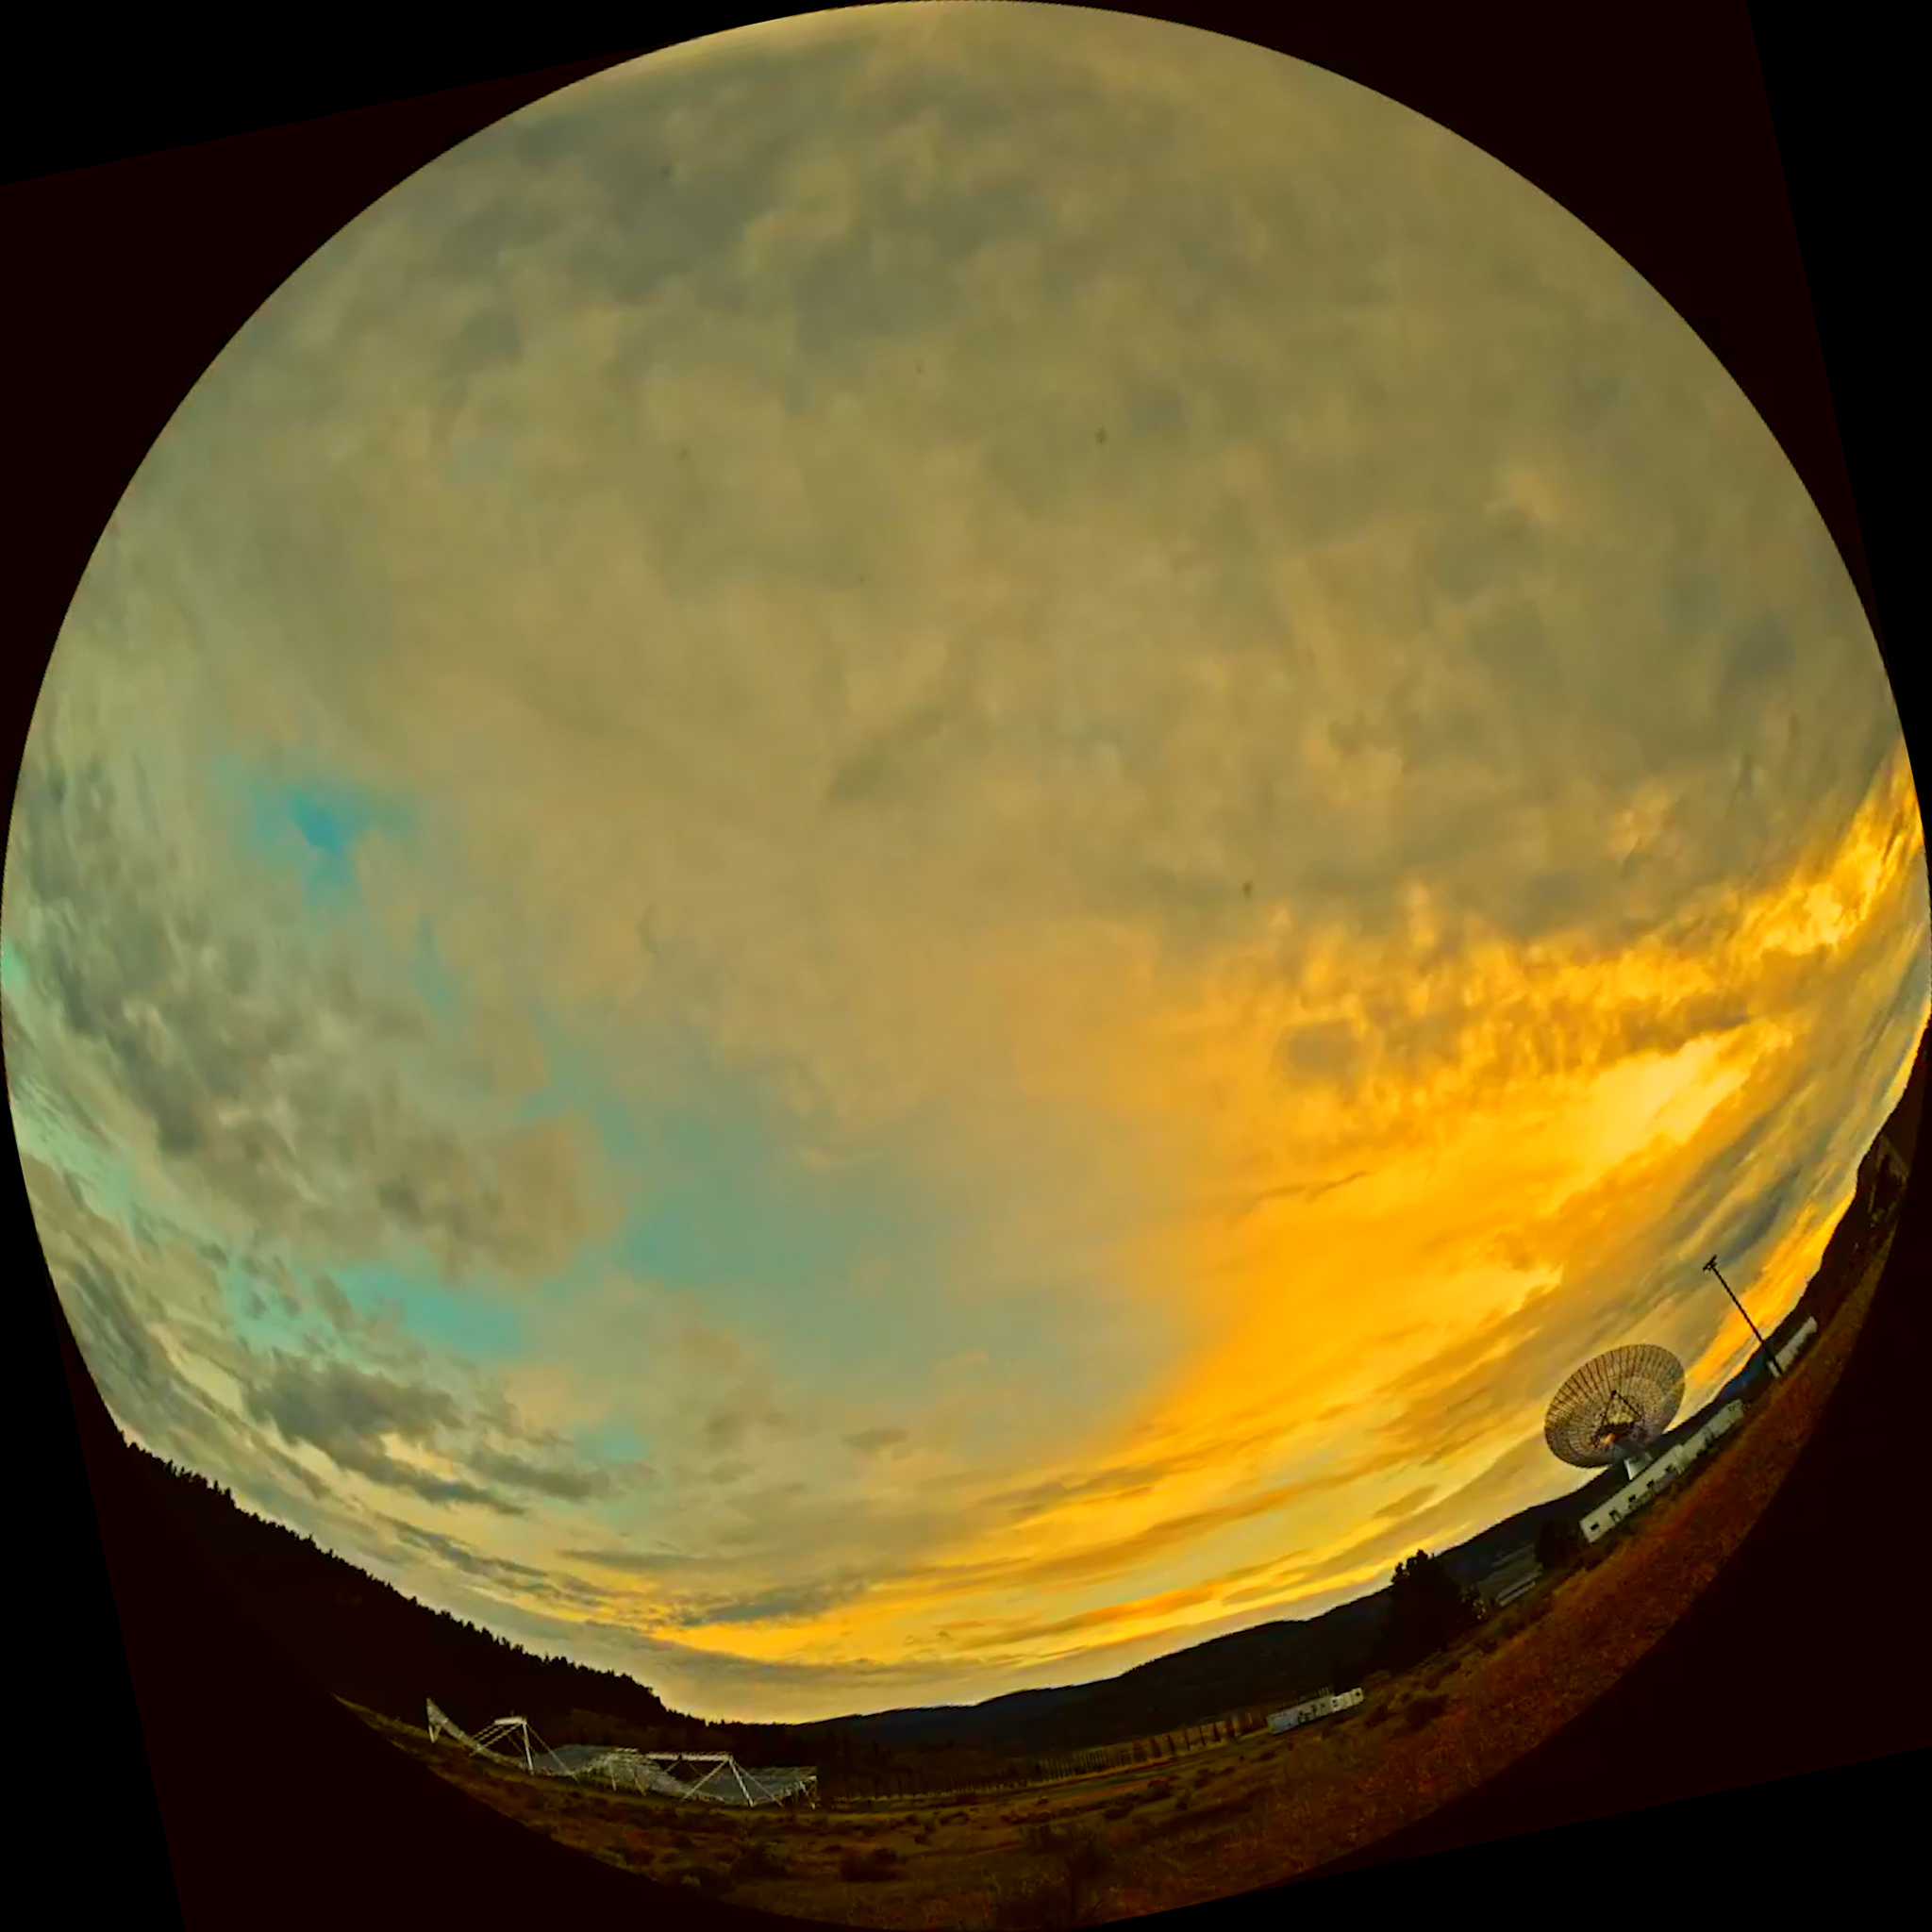
\includegraphics[width=0.3\textwidth]{Planetarium/figures/script_shots/shot1.jpg}} \vspace{0.1cm}\\

\hline

\textit{Beyond the hundreds of billions of stars that make up our own galaxy, the Milky Way; we see many other galaxies, each with hundreds of billions of stars of their own. }& 

\raisebox{-\totalheight}{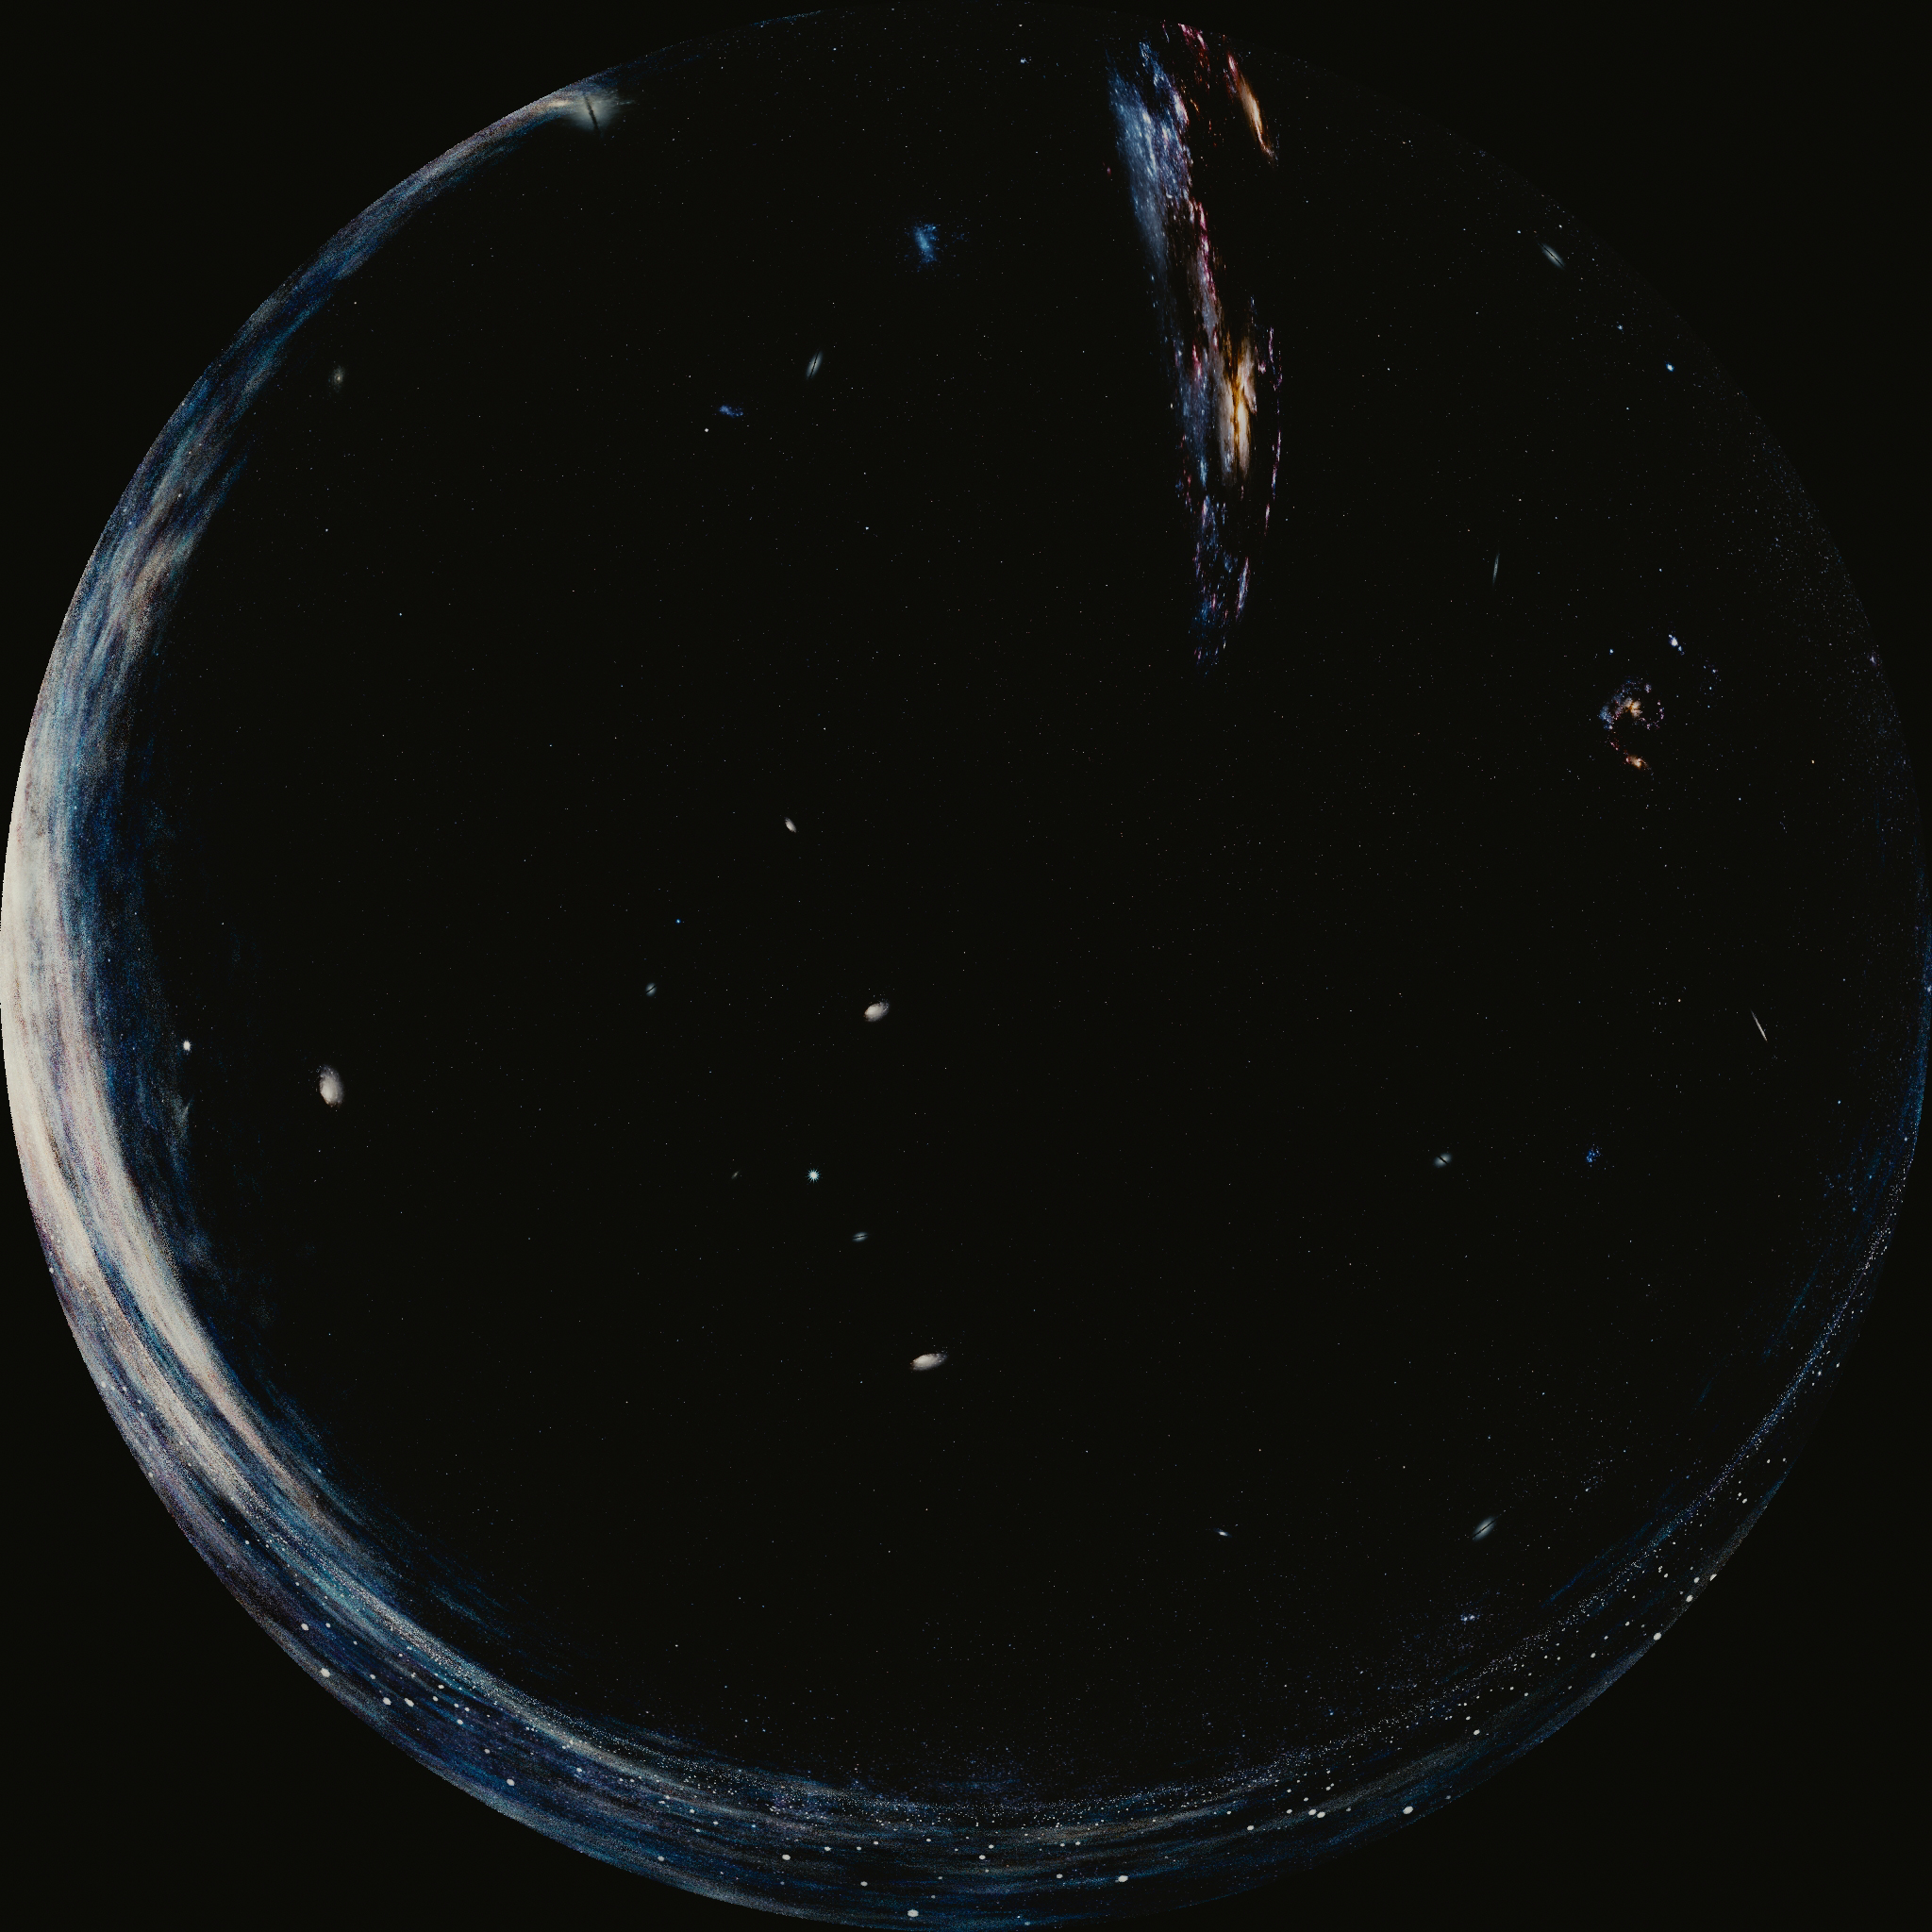
\includegraphics[width=0.3\textwidth]{Planetarium/figures/script_shots/shot2.jpg}} \vspace{0.1cm}\\

\hline

\textit{Because light has a set speed, the light from these more distant galaxies takes longer to reach Earth than the light from our own galaxy. Therefore, we are seeing these galaxies as they were long ago. }& 

\raisebox{-\totalheight}{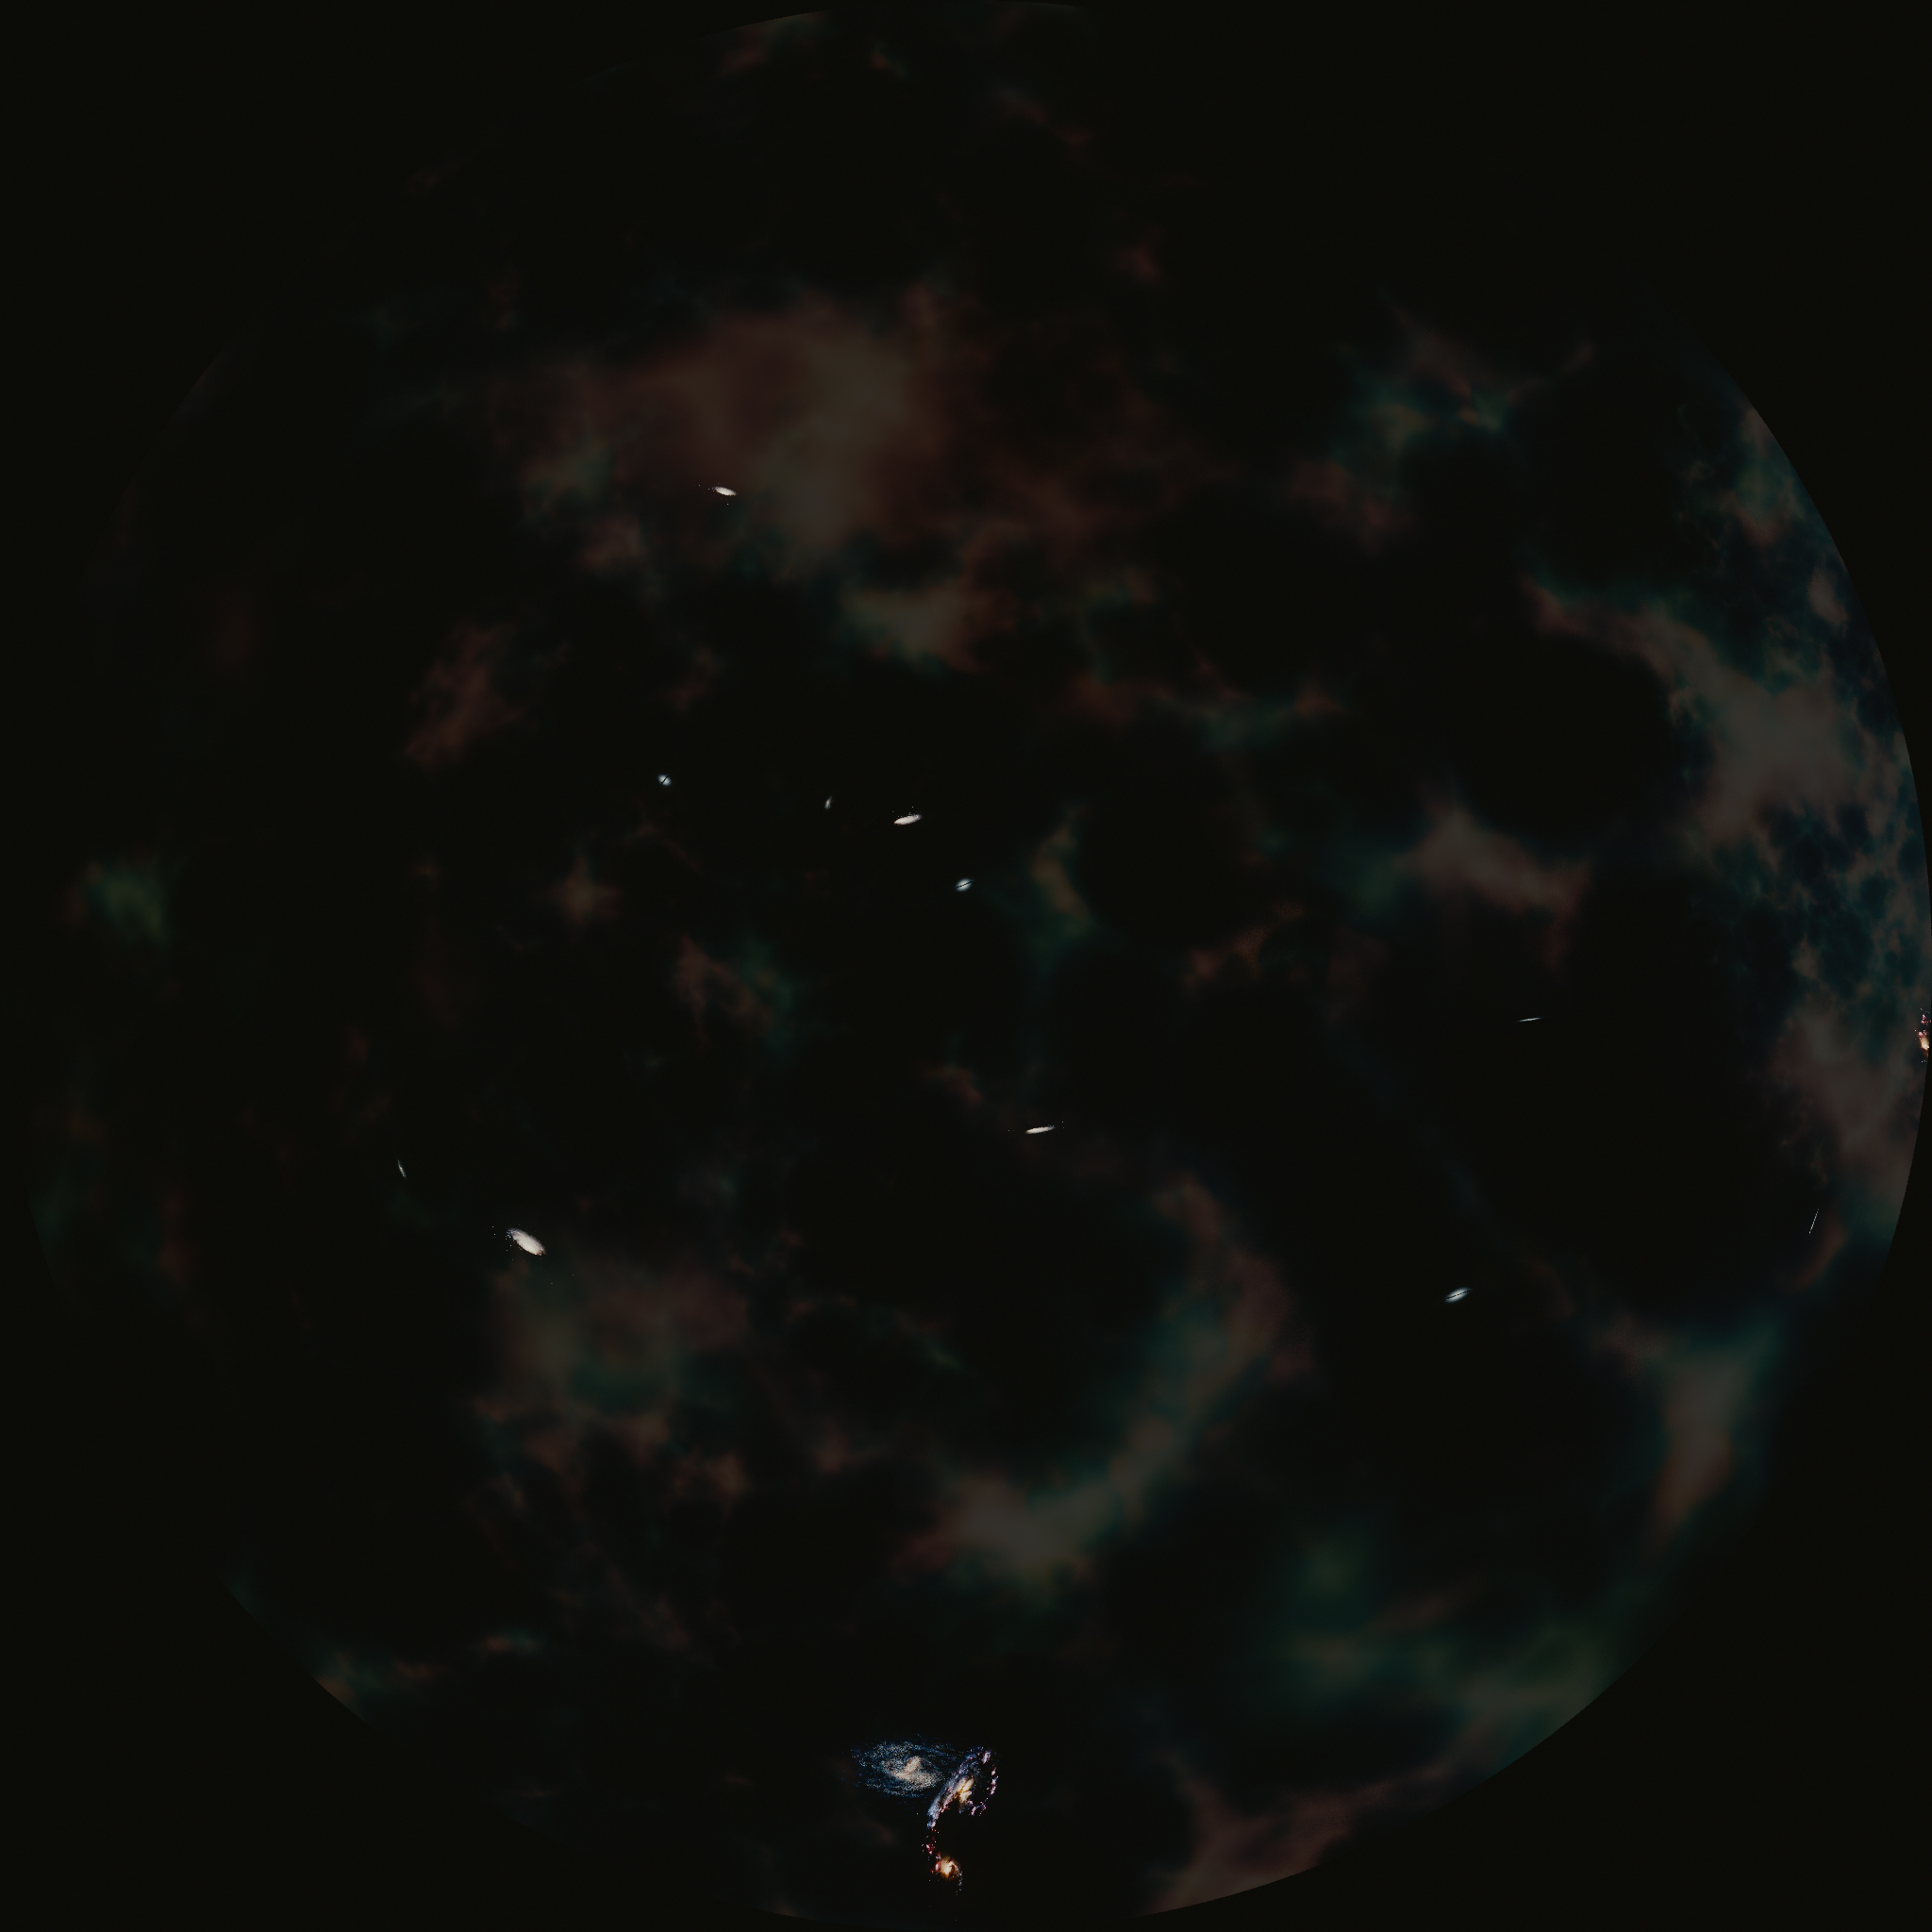
\includegraphics[width=0.3\textwidth]{Planetarium/figures/script_shots/shot3.jpg}} \vspace{0.1cm}\\

\hline

\textit{If we keep looking further and further away, and therefore further back in time, eventually we stop seeing anything. This is because the very distant galaxies are not bright enough for us to see, or they haven't even formed stars yet. }& 

\raisebox{-\totalheight}{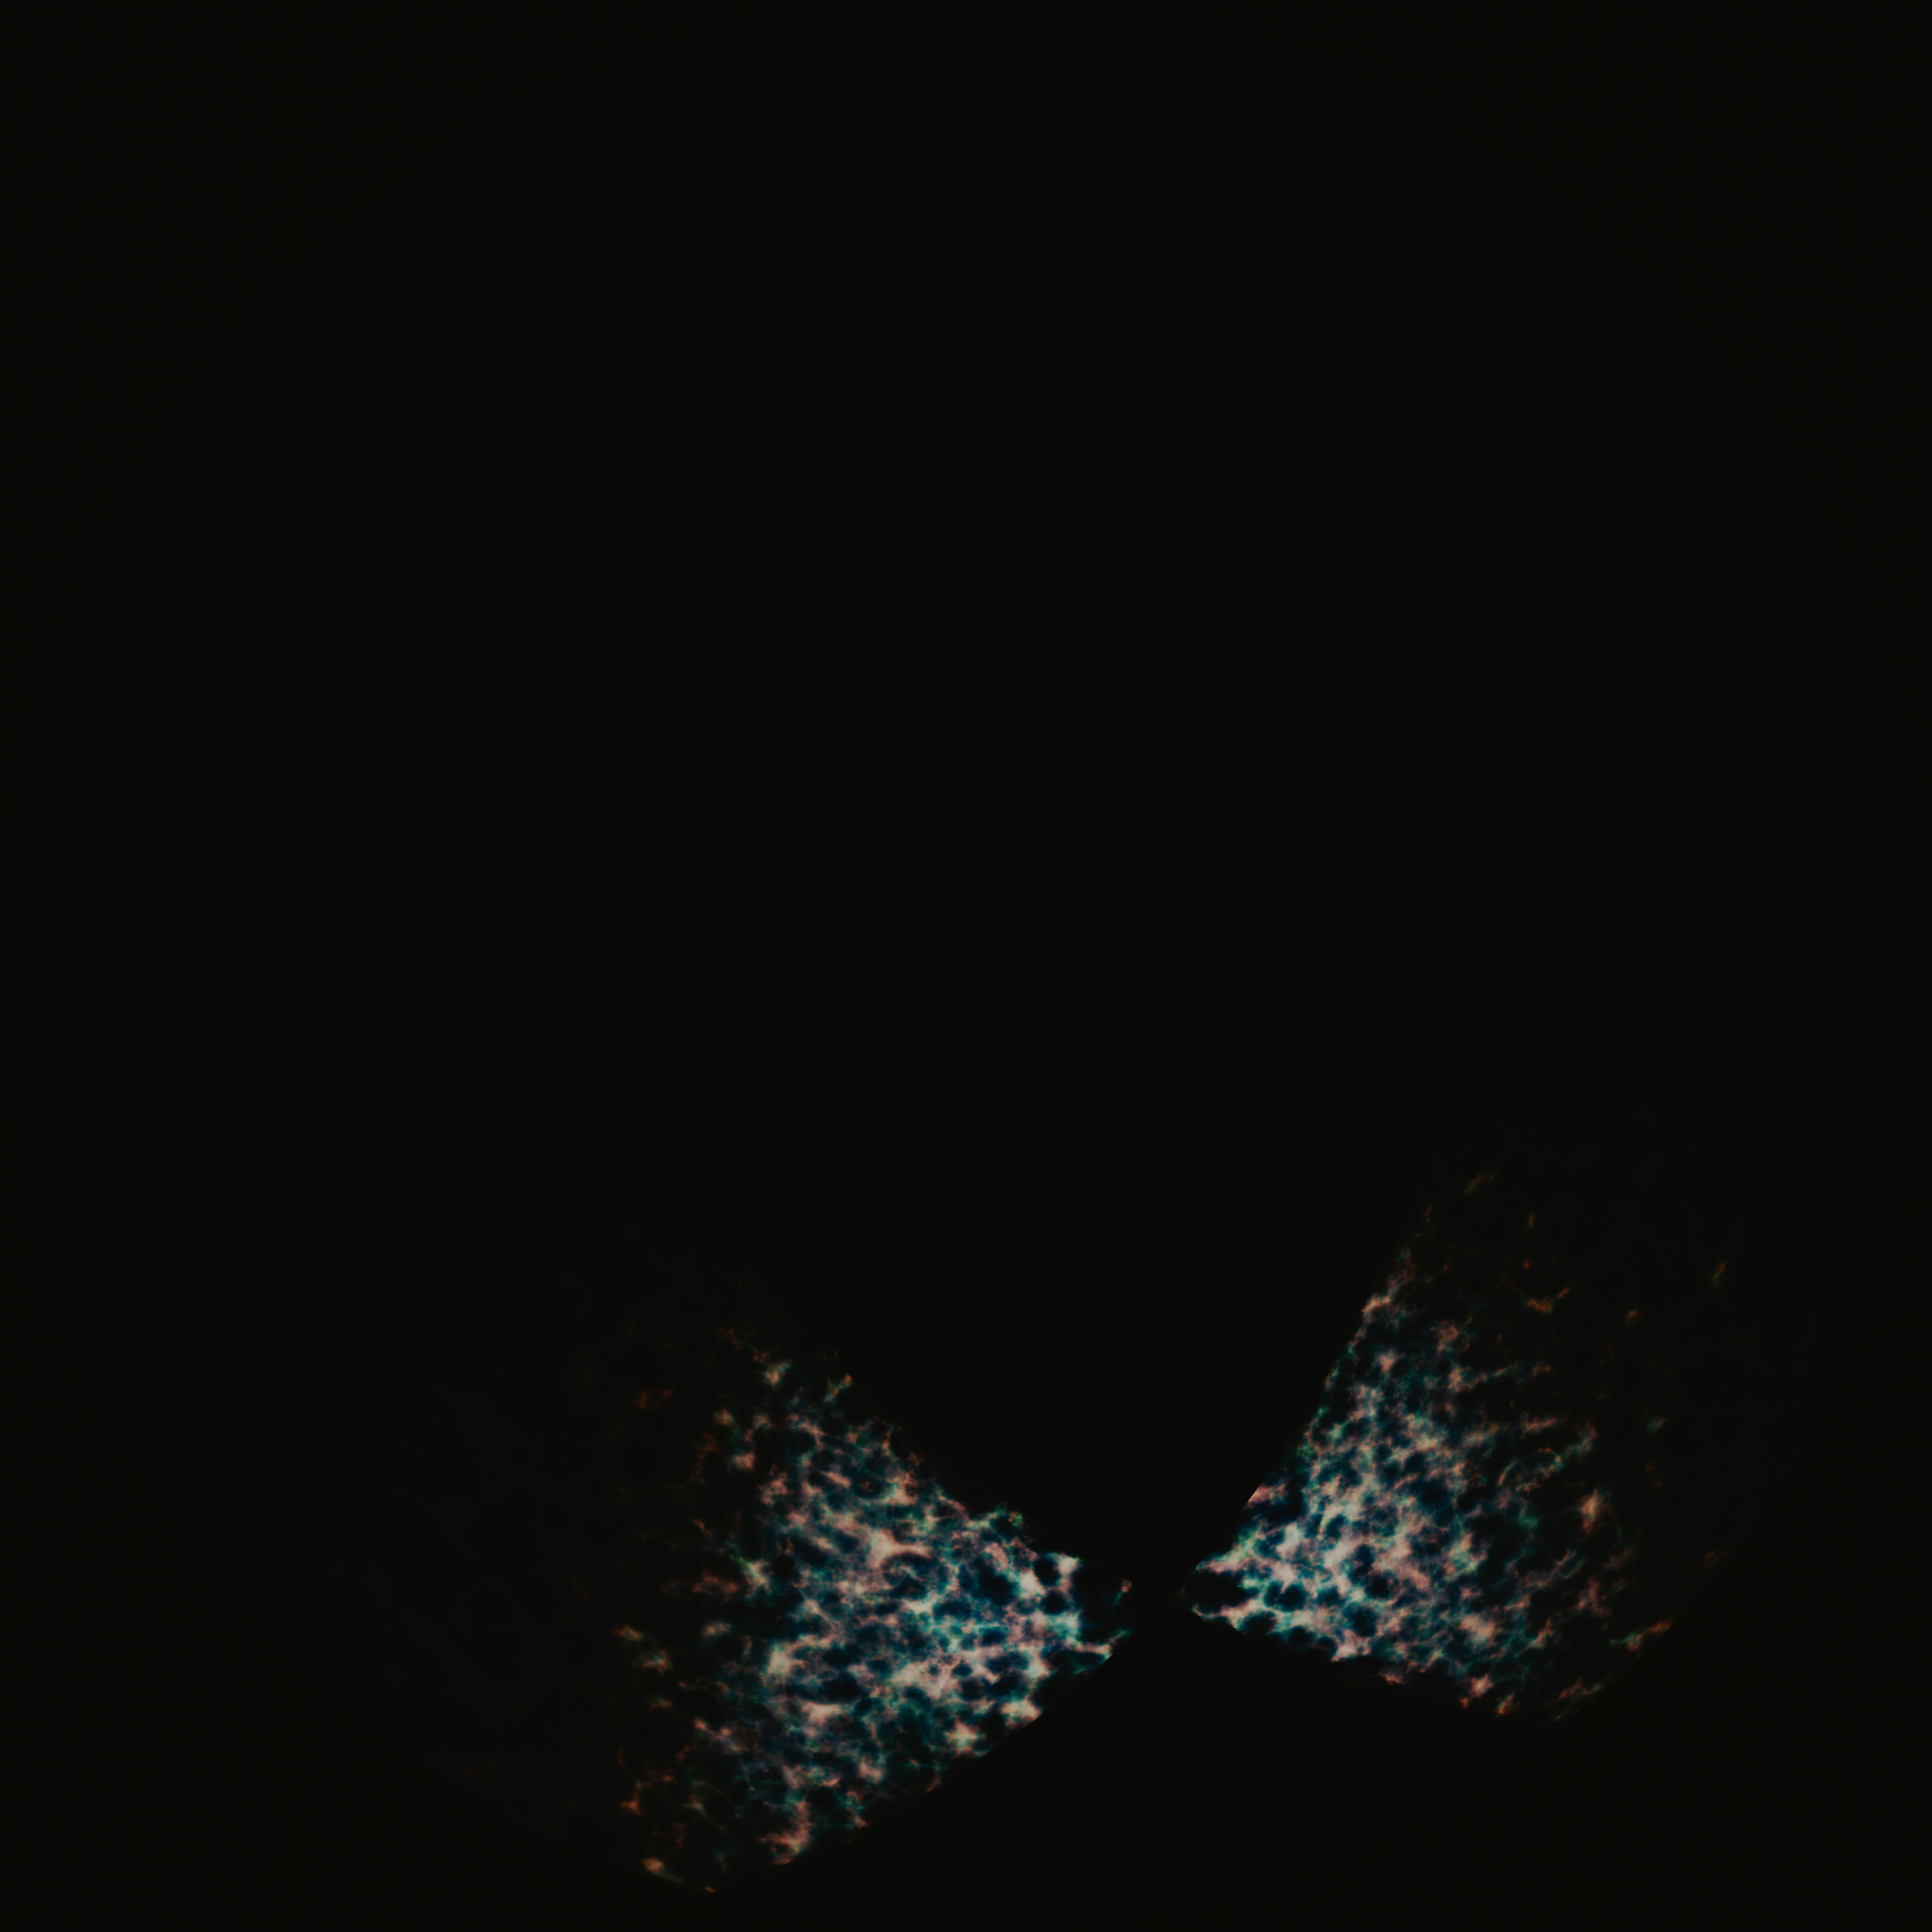
\includegraphics[width=0.3\textwidth]{Planetarium/figures/script_shots/shot4.jpg}} \vspace{0.1cm}\\

\hline

\textit{To study these very distant, and very young galaxies, scientists like me need a new way to see the sky, we need the Hydrogen Sky.  }& 

\raisebox{-\totalheight}{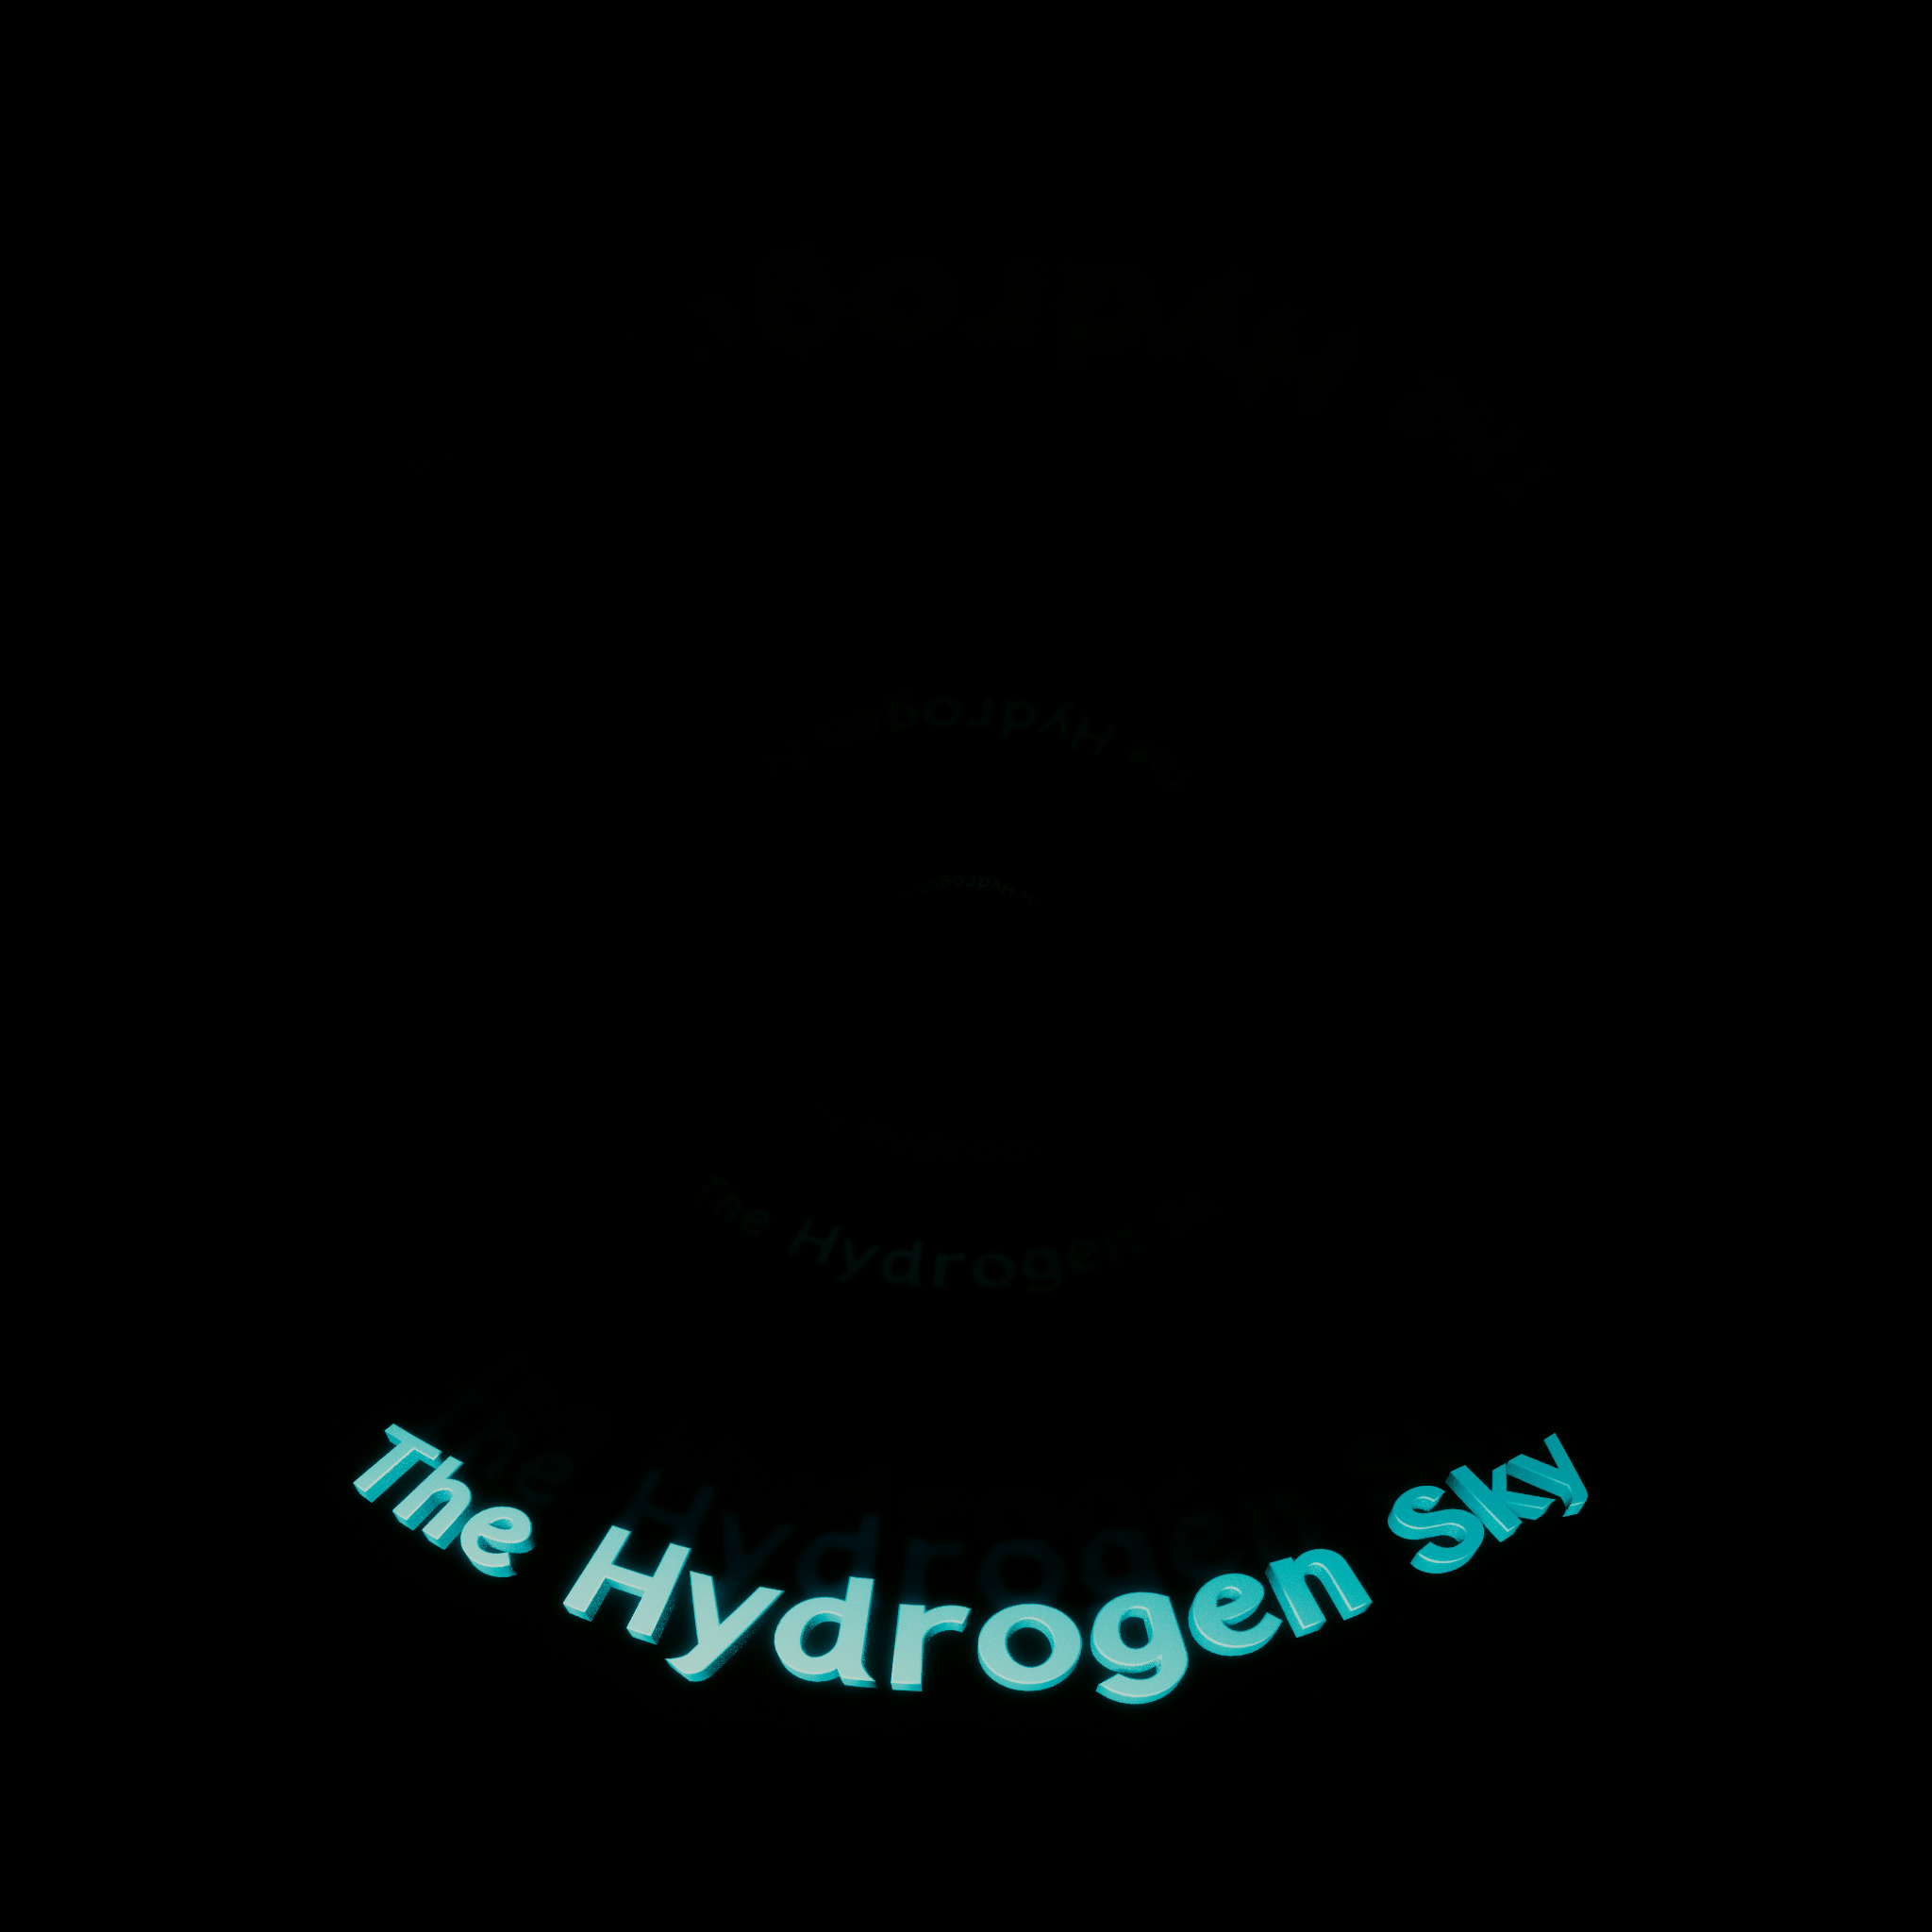
\includegraphics[width=0.3\textwidth]{Planetarium/figures/script_shots/shot5.jpg}}\vspace{0.1cm} \\

\hline

\textit{From early times, photons of light were able to freely travel through the universe. } &

\raisebox{-\totalheight}{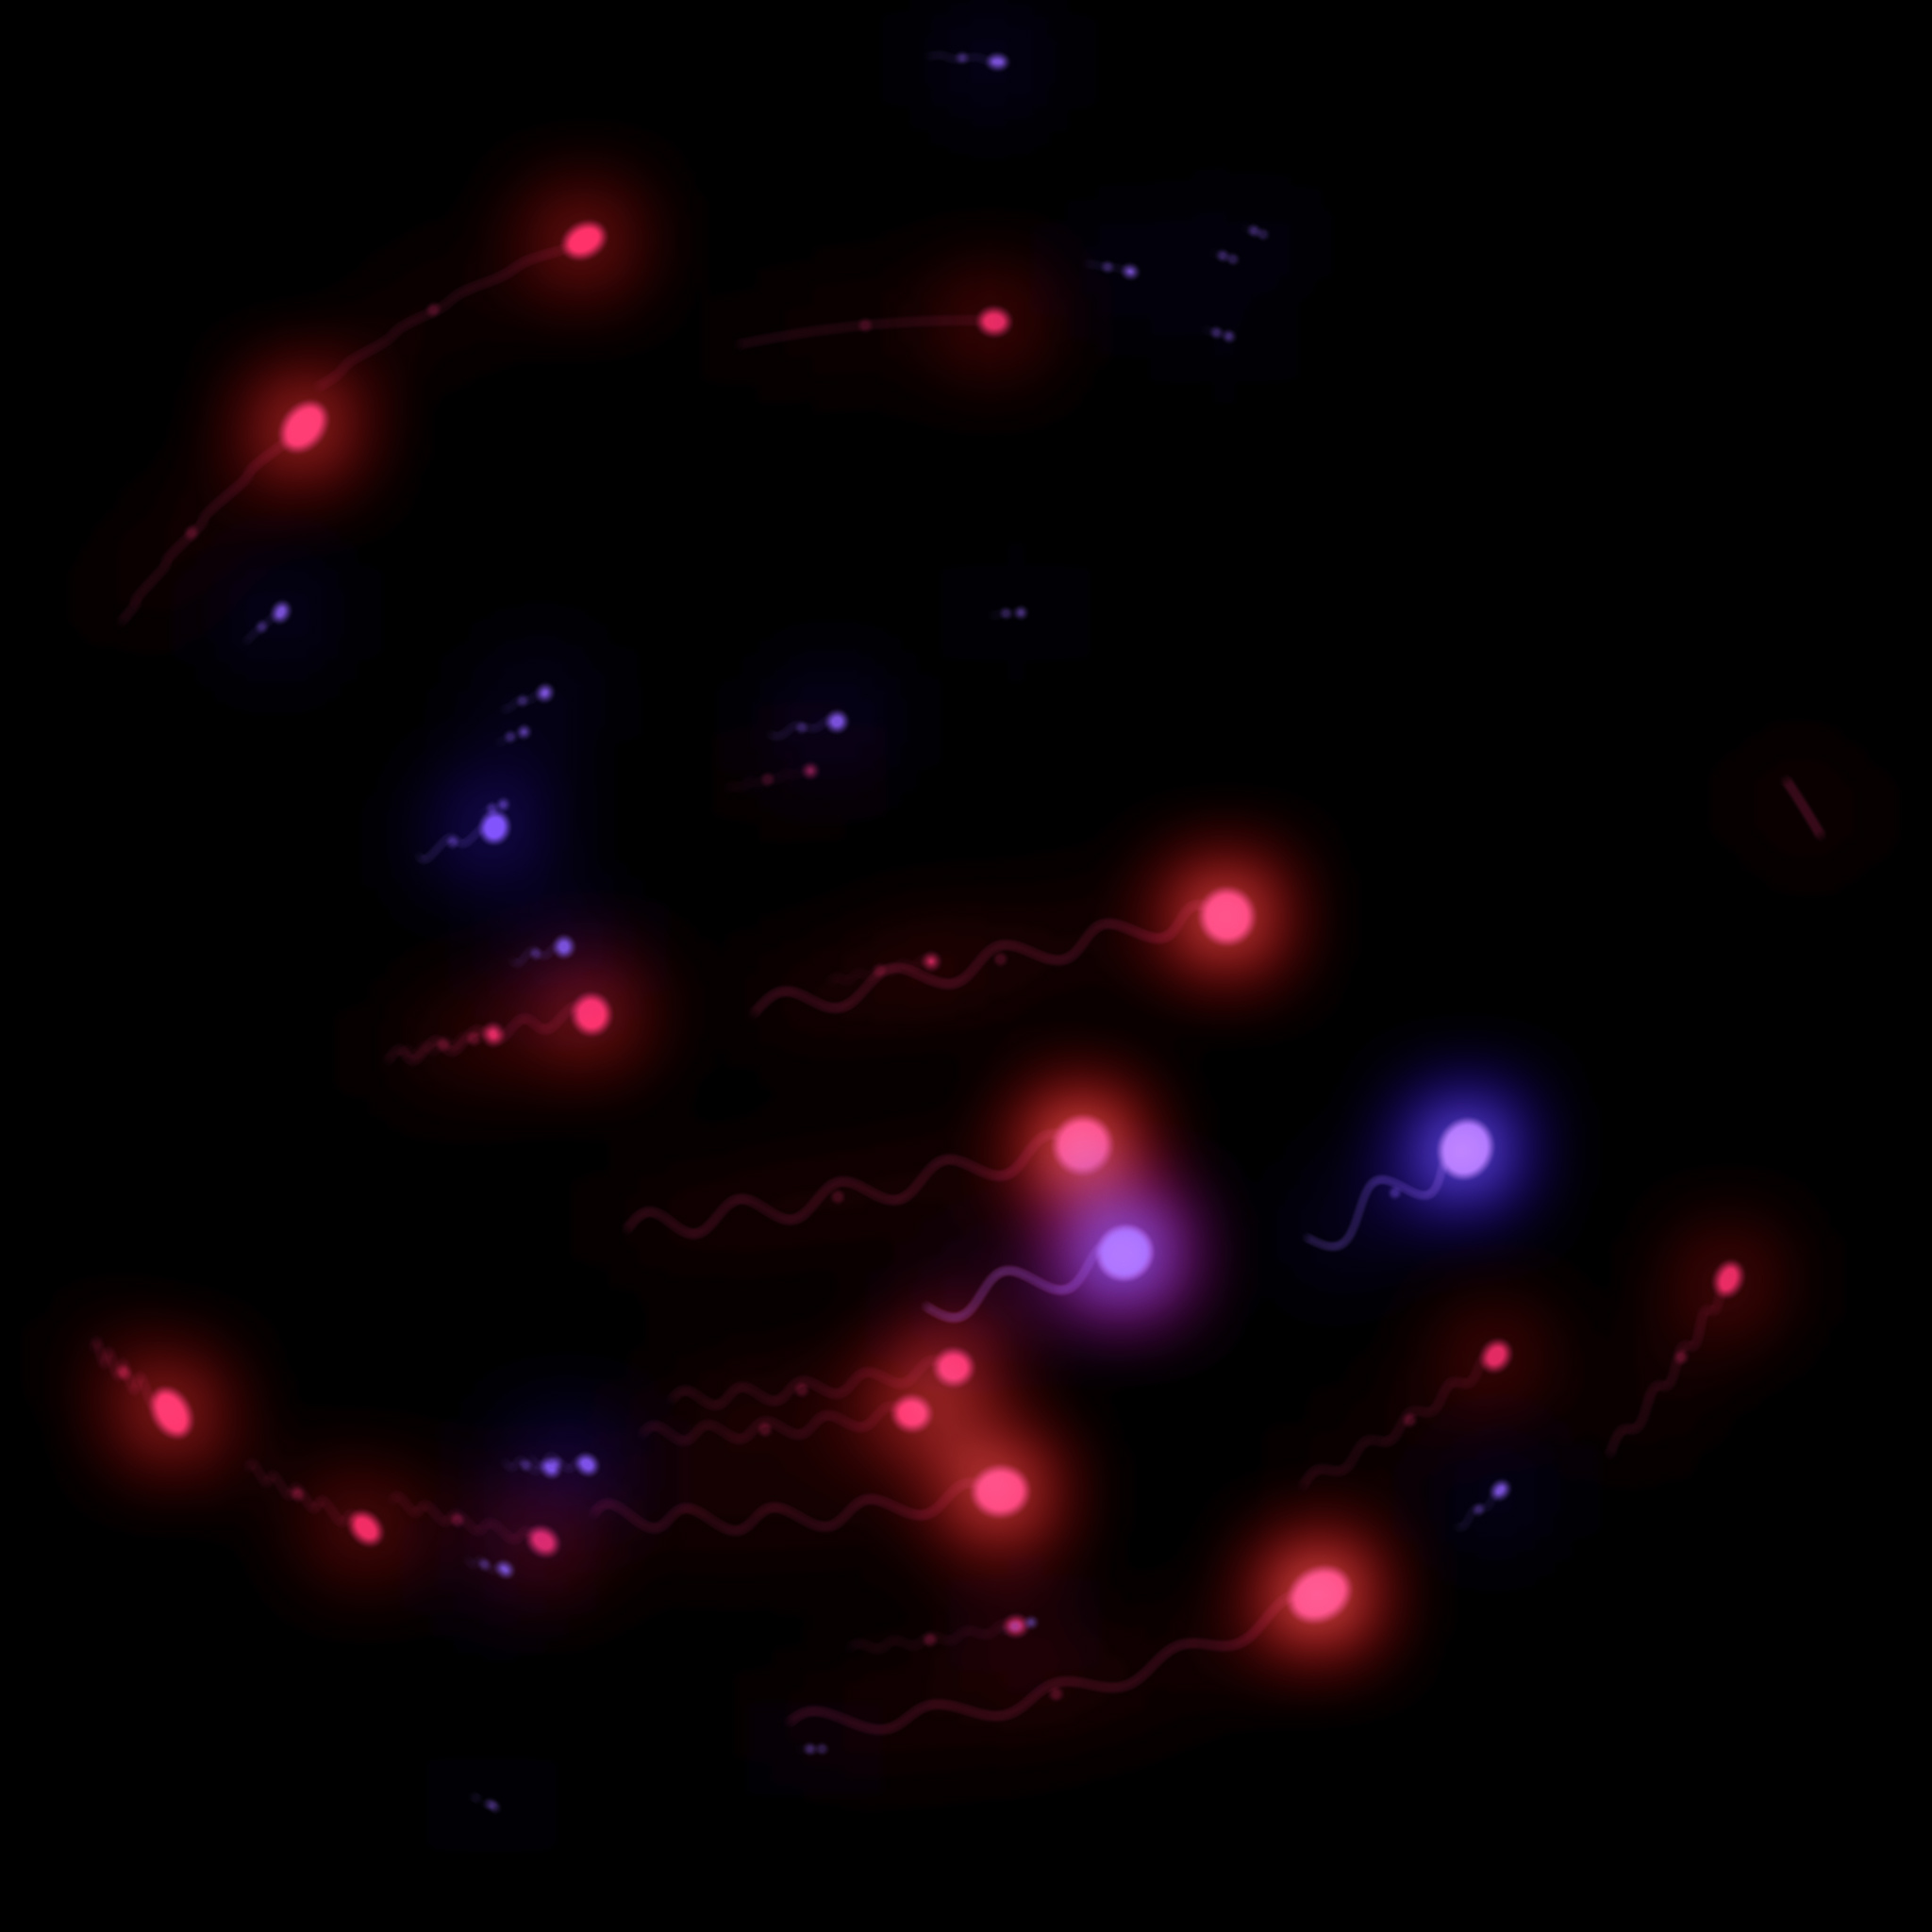
\includegraphics[width=0.3\textwidth]{Planetarium/figures/script_shots/shot6.jpg}} \vspace{0.1cm}\\

\hline

\textit{These photons each had a specific wavelength, or color. For some, that wavelength was 21 centimeters, or a little over 8 inches. }& 

\raisebox{-\totalheight}{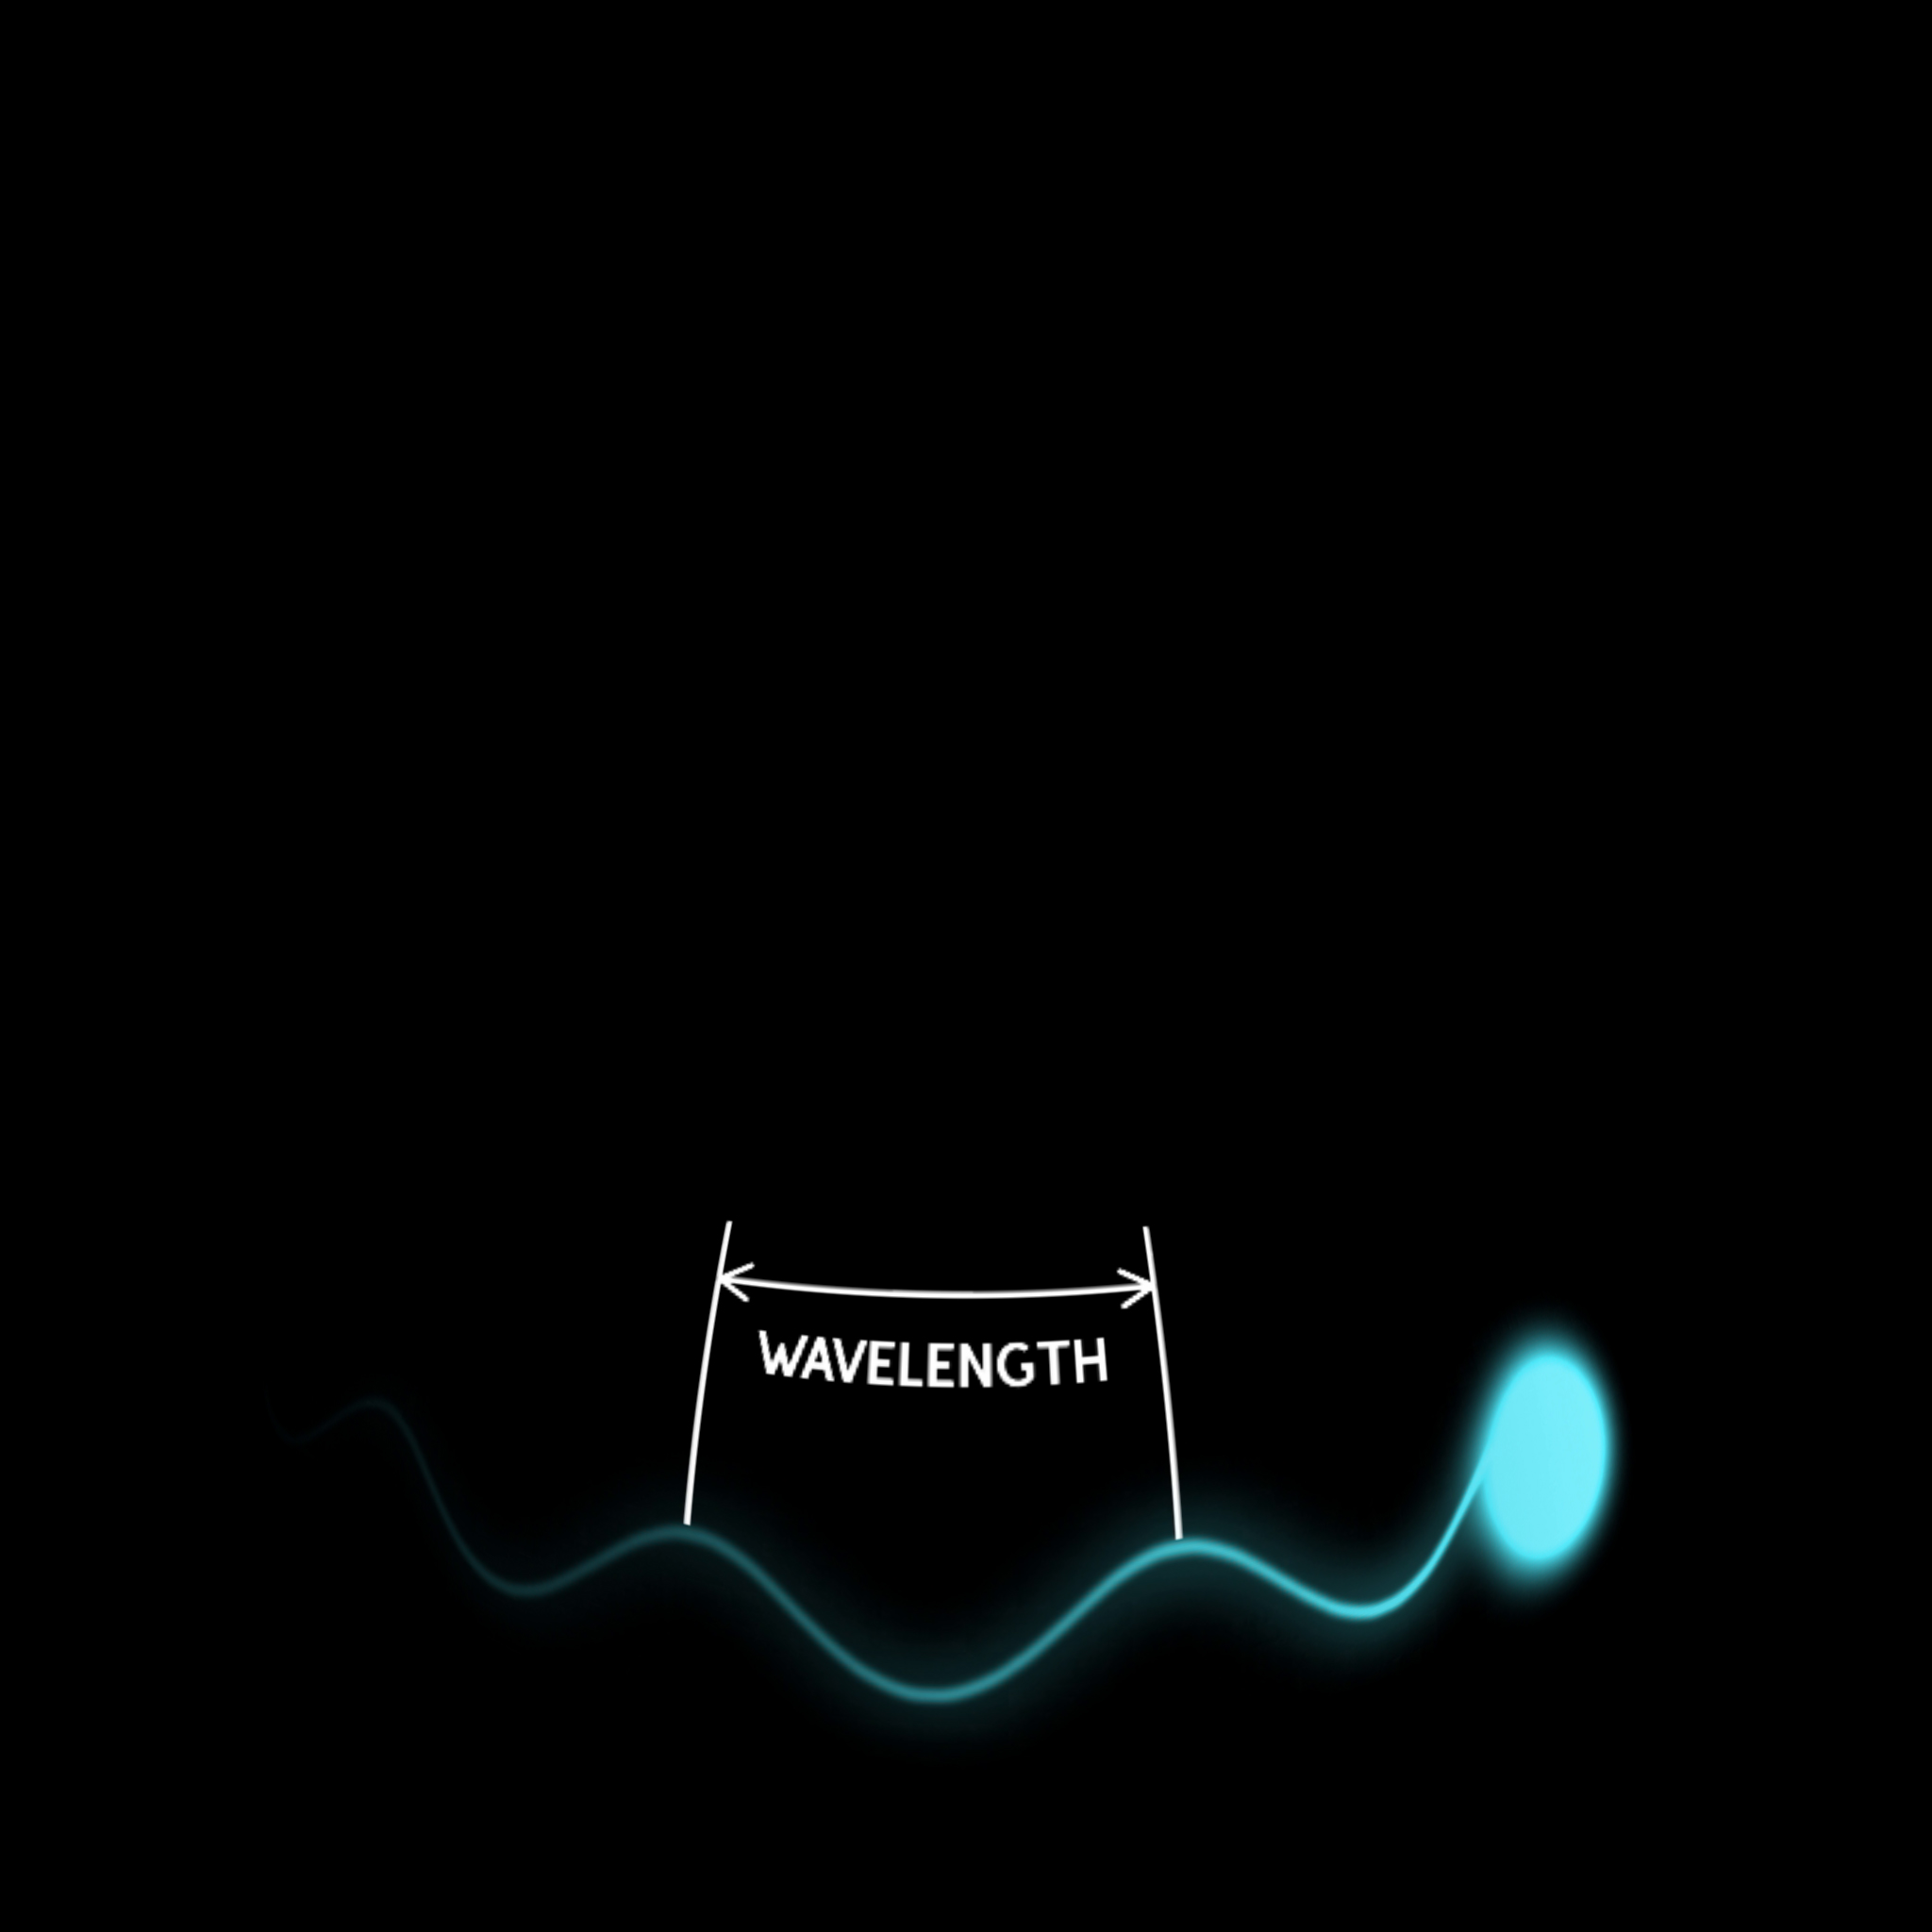
\includegraphics[width=0.3\textwidth]{Planetarium/figures/script_shots/shot7.jpg}} \vspace{0.1cm}\\

\hline

\textit{As they travelled, photons passed through galaxies and the clouds of Hydrogen gas that surrounded the galaxies.} & 

\raisebox{-\totalheight}{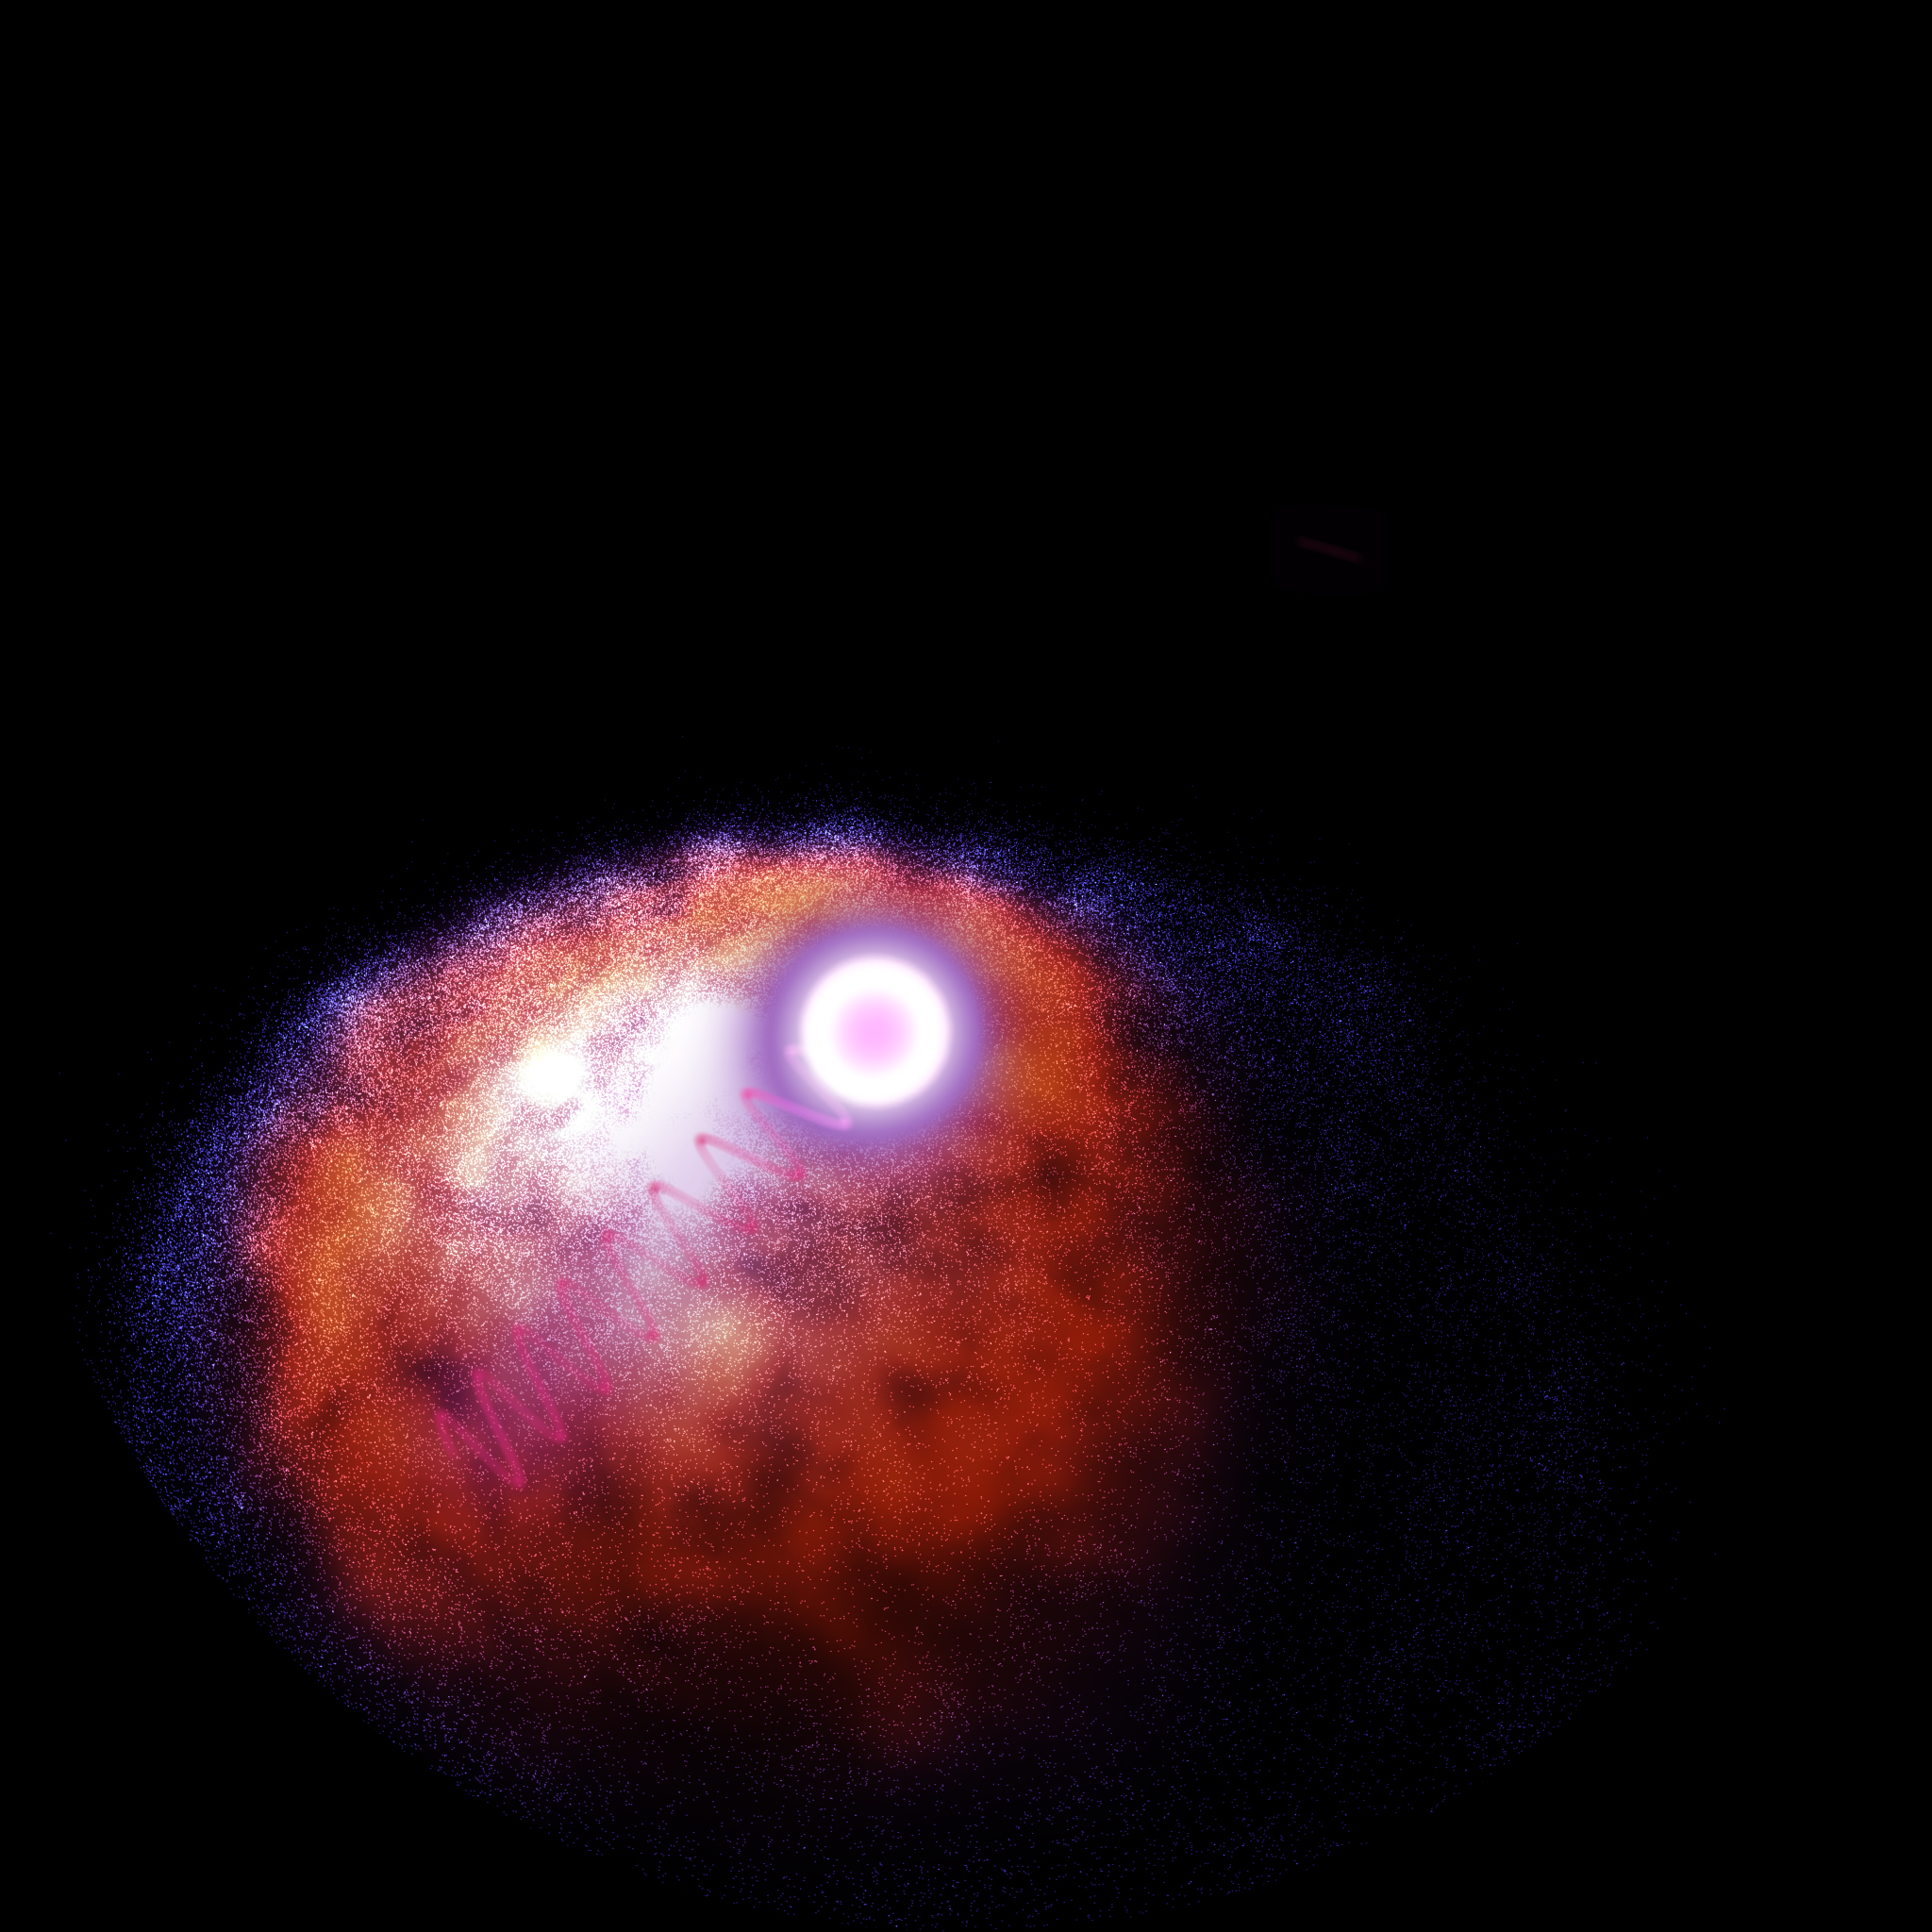
\includegraphics[width=0.3\textwidth]{Planetarium/figures/script_shots/shot8.jpg}} \vspace{0.1cm}\\

\hline

\textit{Inside these clouds are many trillions of individual Hydrogen atoms. Each atom has a proton and an electron.  }& 

\raisebox{-\totalheight}{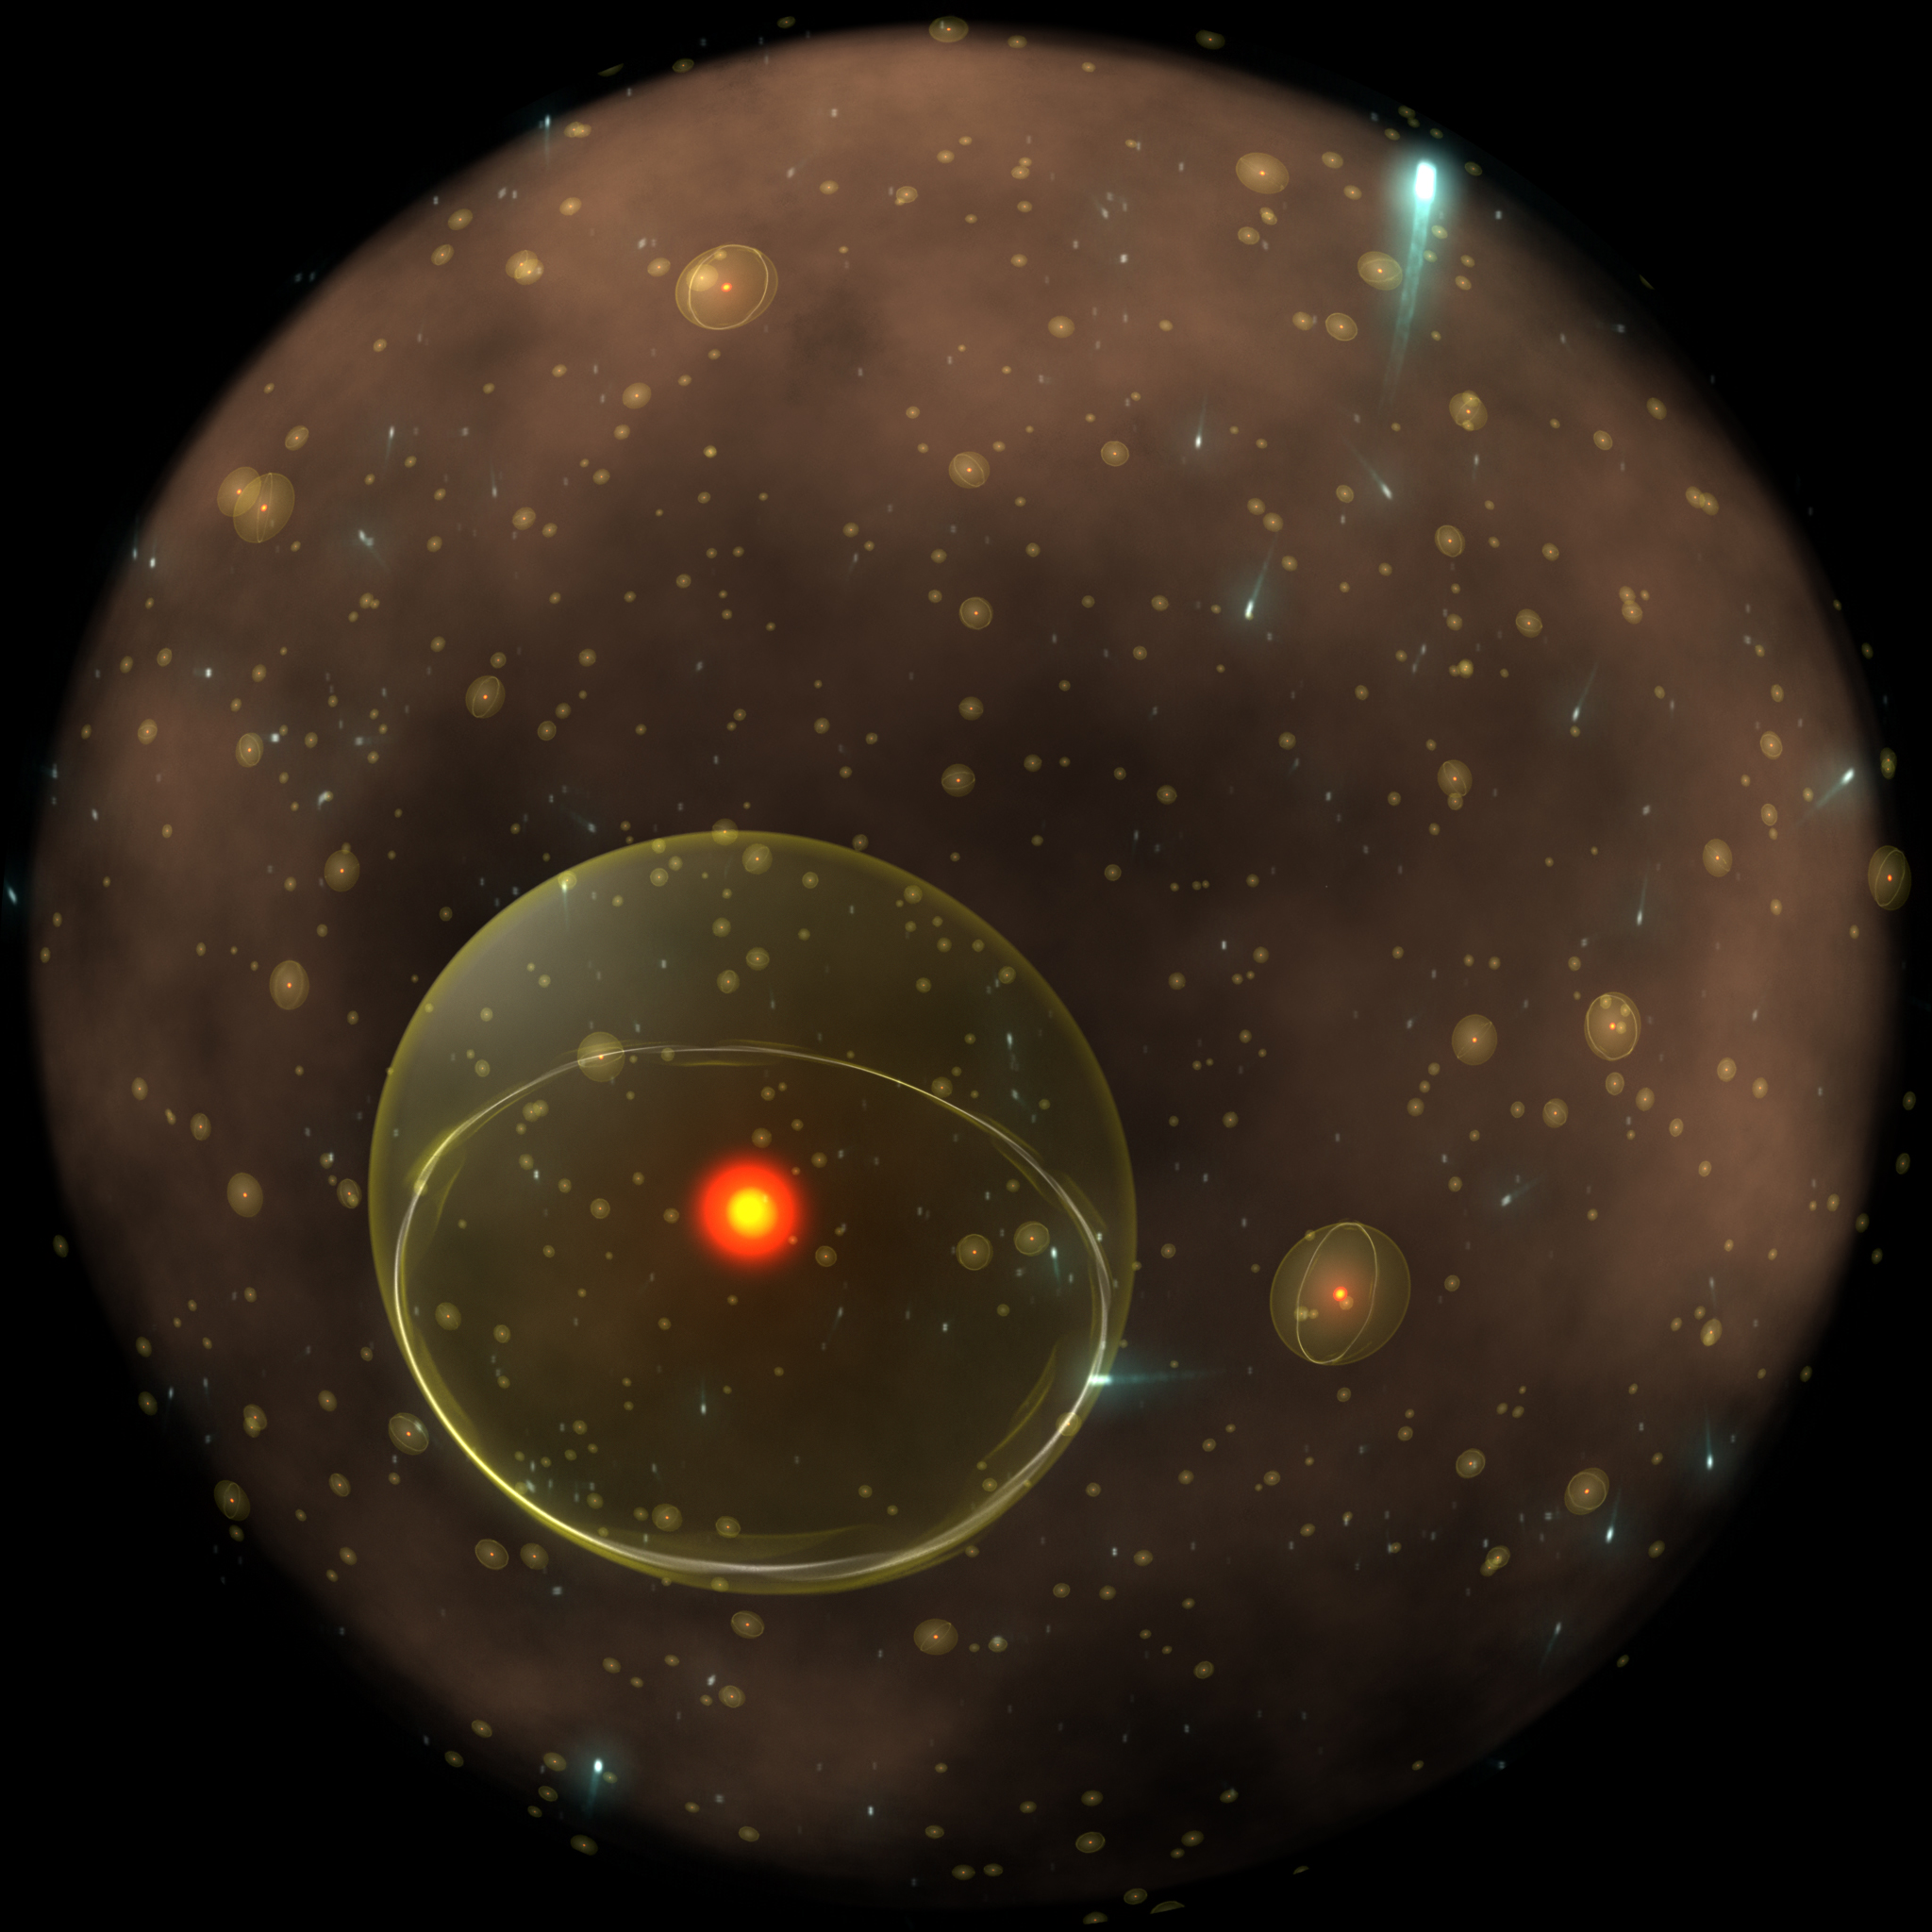
\includegraphics[width=0.3\textwidth]{Planetarium/figures/script_shots/shot9.jpg}}\vspace{0.1cm}\\

\hline

\textit{Both the proton and the electron have a special property called spin. This spin has two directions, clockwise and counter-clockwise.  }& 

\raisebox{-\totalheight}{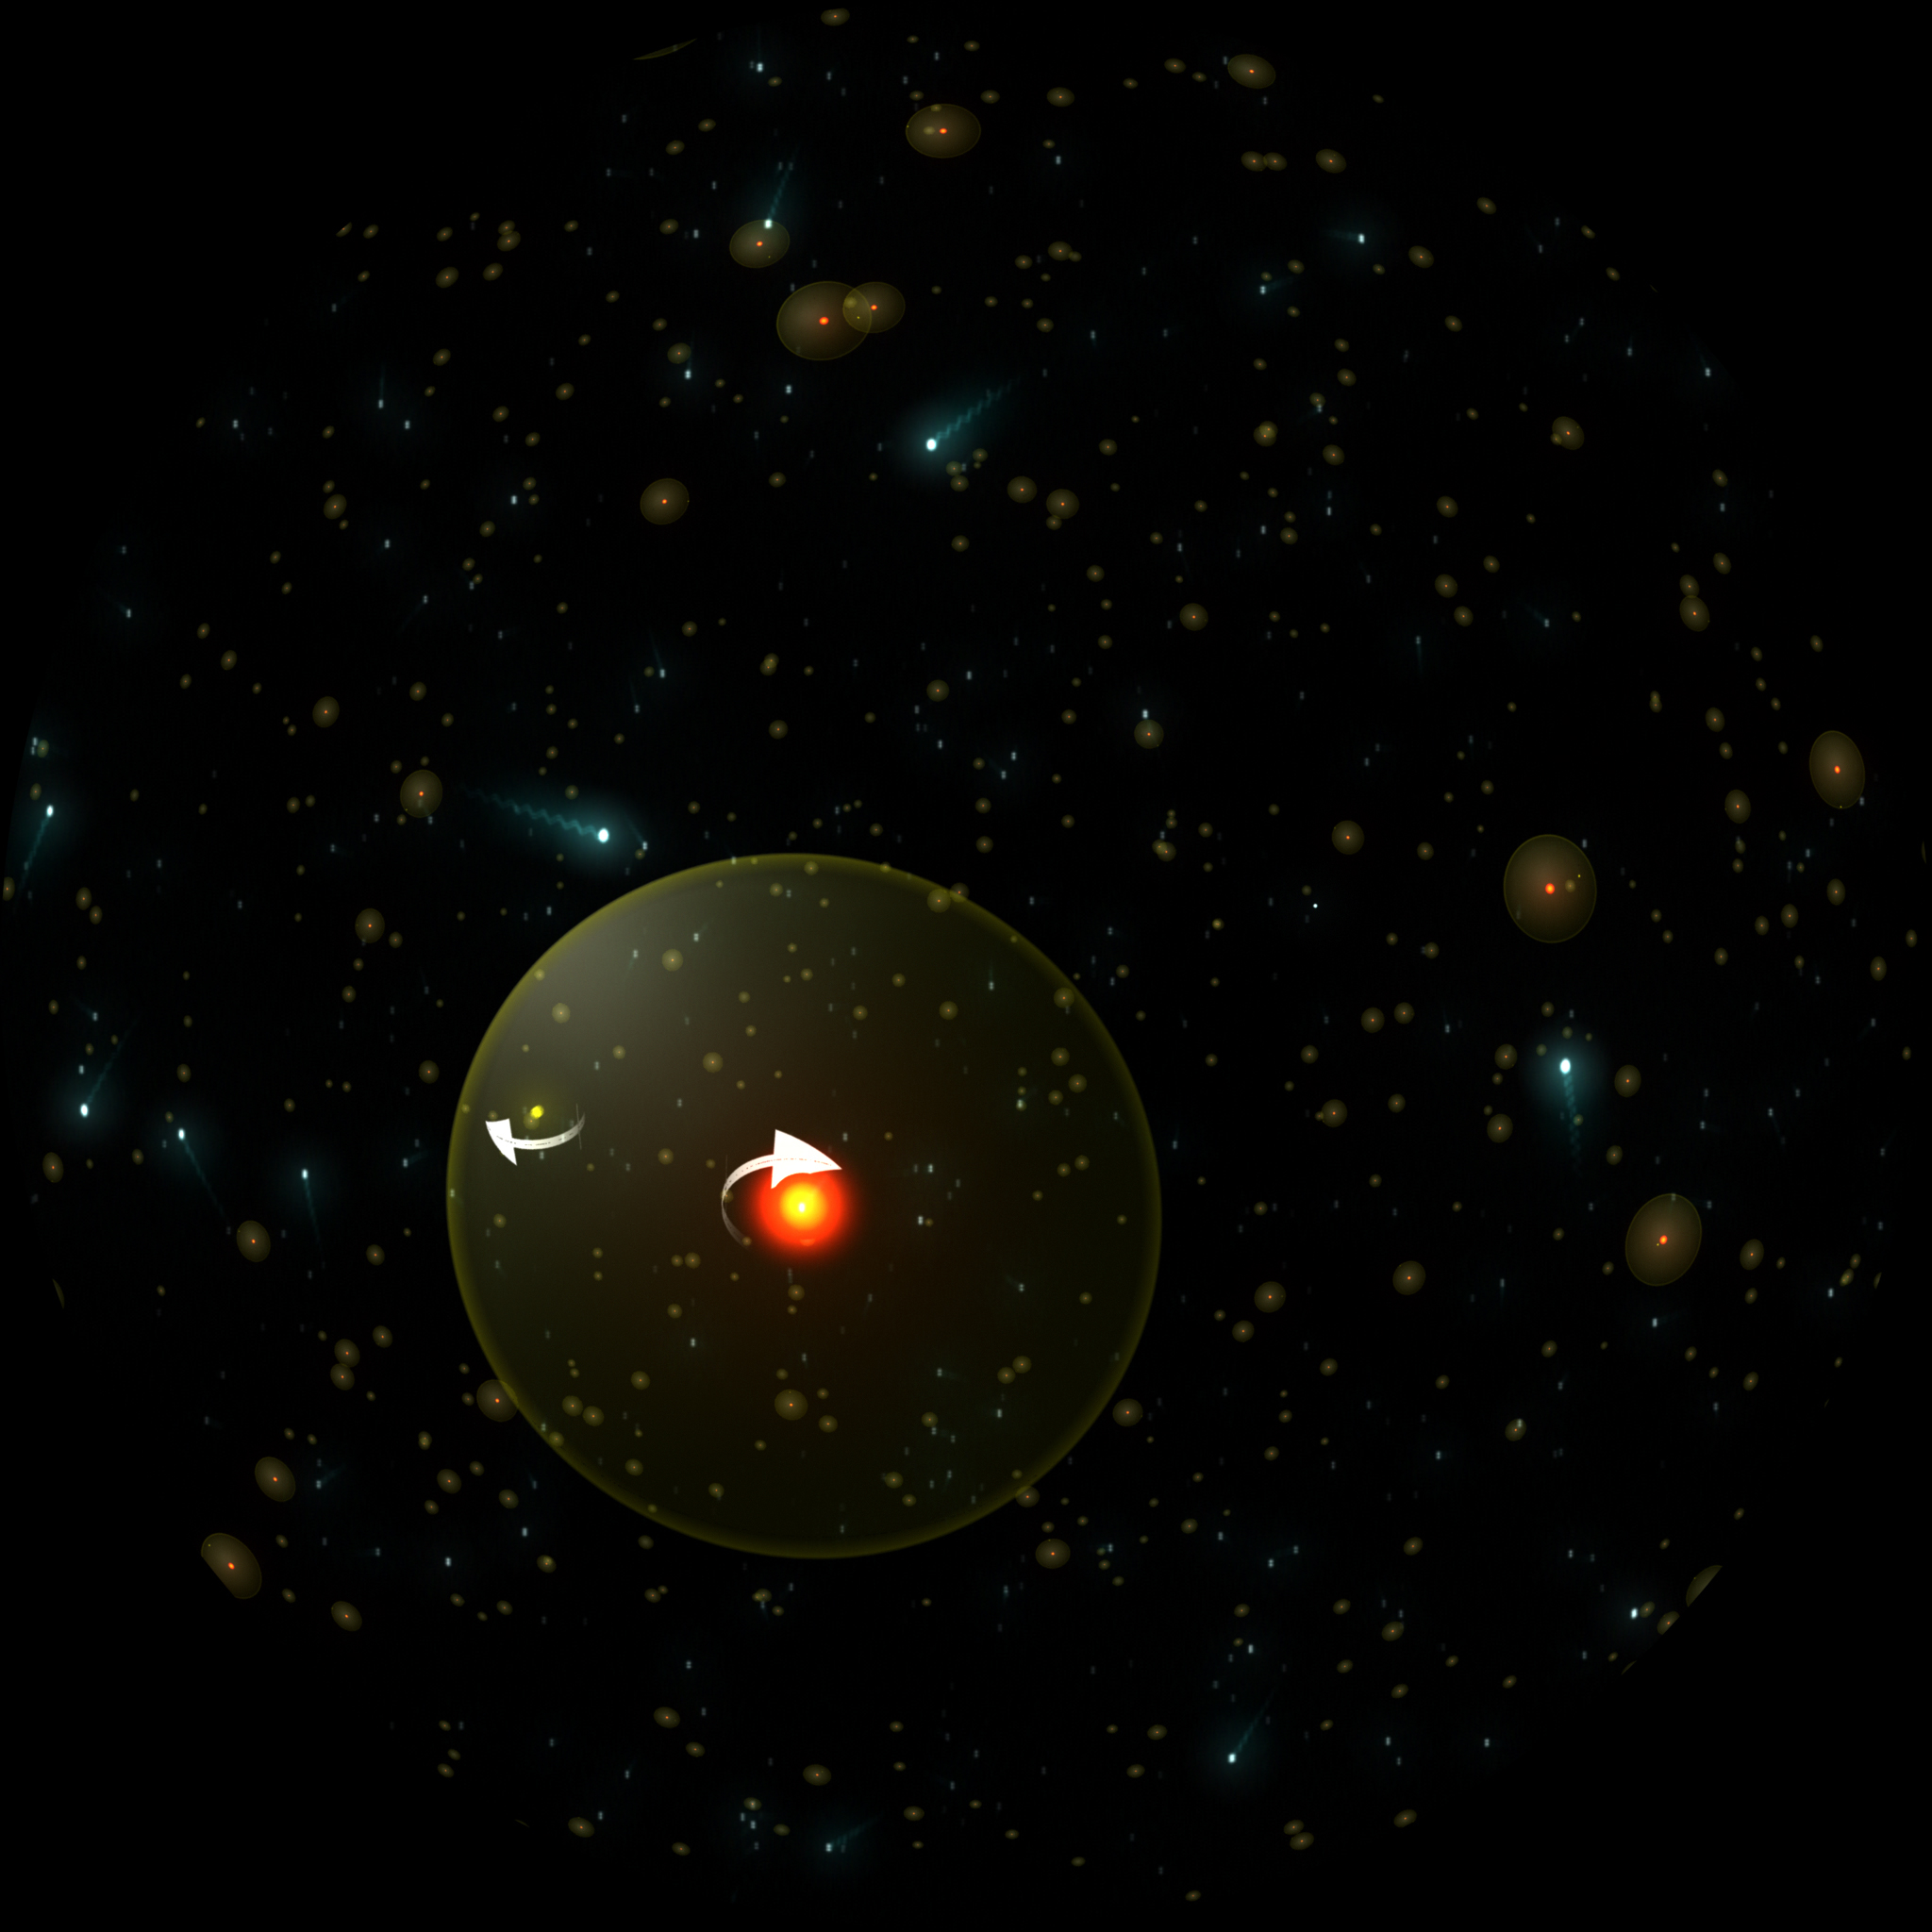
\includegraphics[width=0.3\textwidth]{Planetarium/figures/script_shots/shot10.jpg}}\vspace{0.1cm}\\

\hline

\textit{Photons sometimes collide with these Hydrogen atoms. When they do, one of two things can happen. If the proton and electron spin in the same direction, a spin flips, and two photons fly away. }& 

\raisebox{-\totalheight}{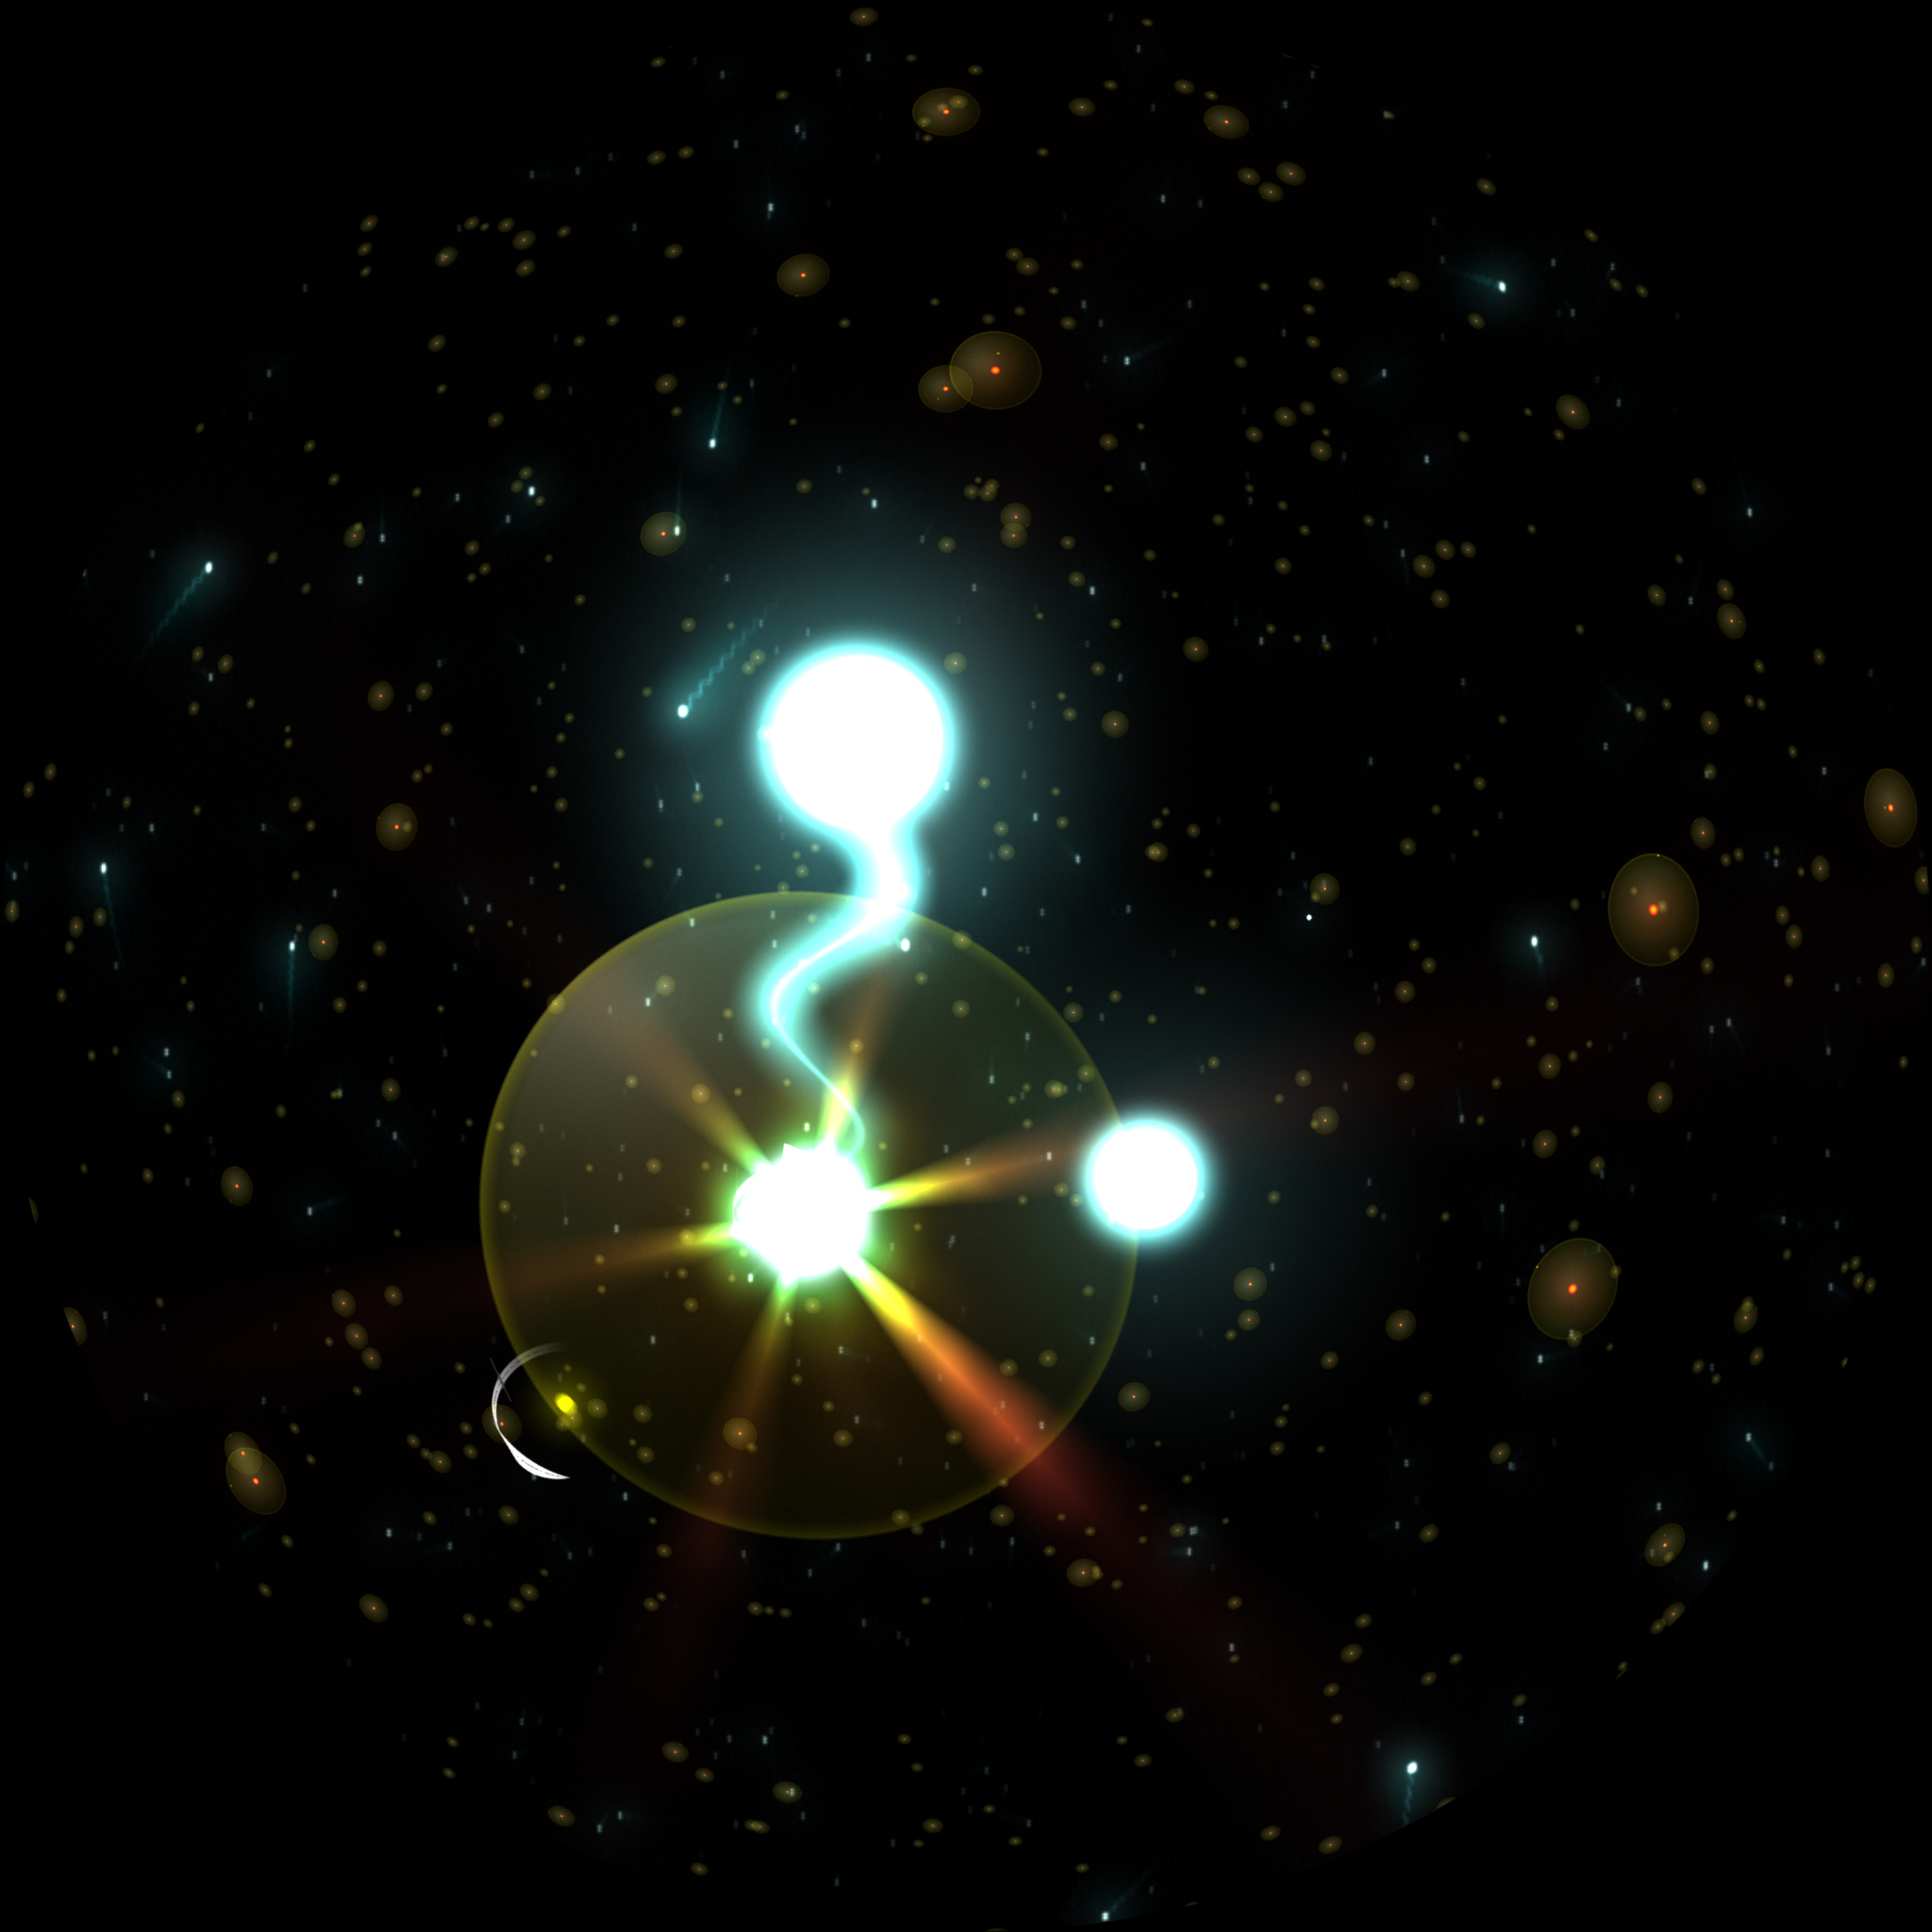
\includegraphics[width=0.3\textwidth]{Planetarium/figures/script_shots/shot11.jpg}}\vspace{0.1cm}\\

\hline

\textit{But, if the electron and proton spin in opposite directions, one of the spins flips and the photon is absorbed by the atom.  }& 

\raisebox{-\totalheight}{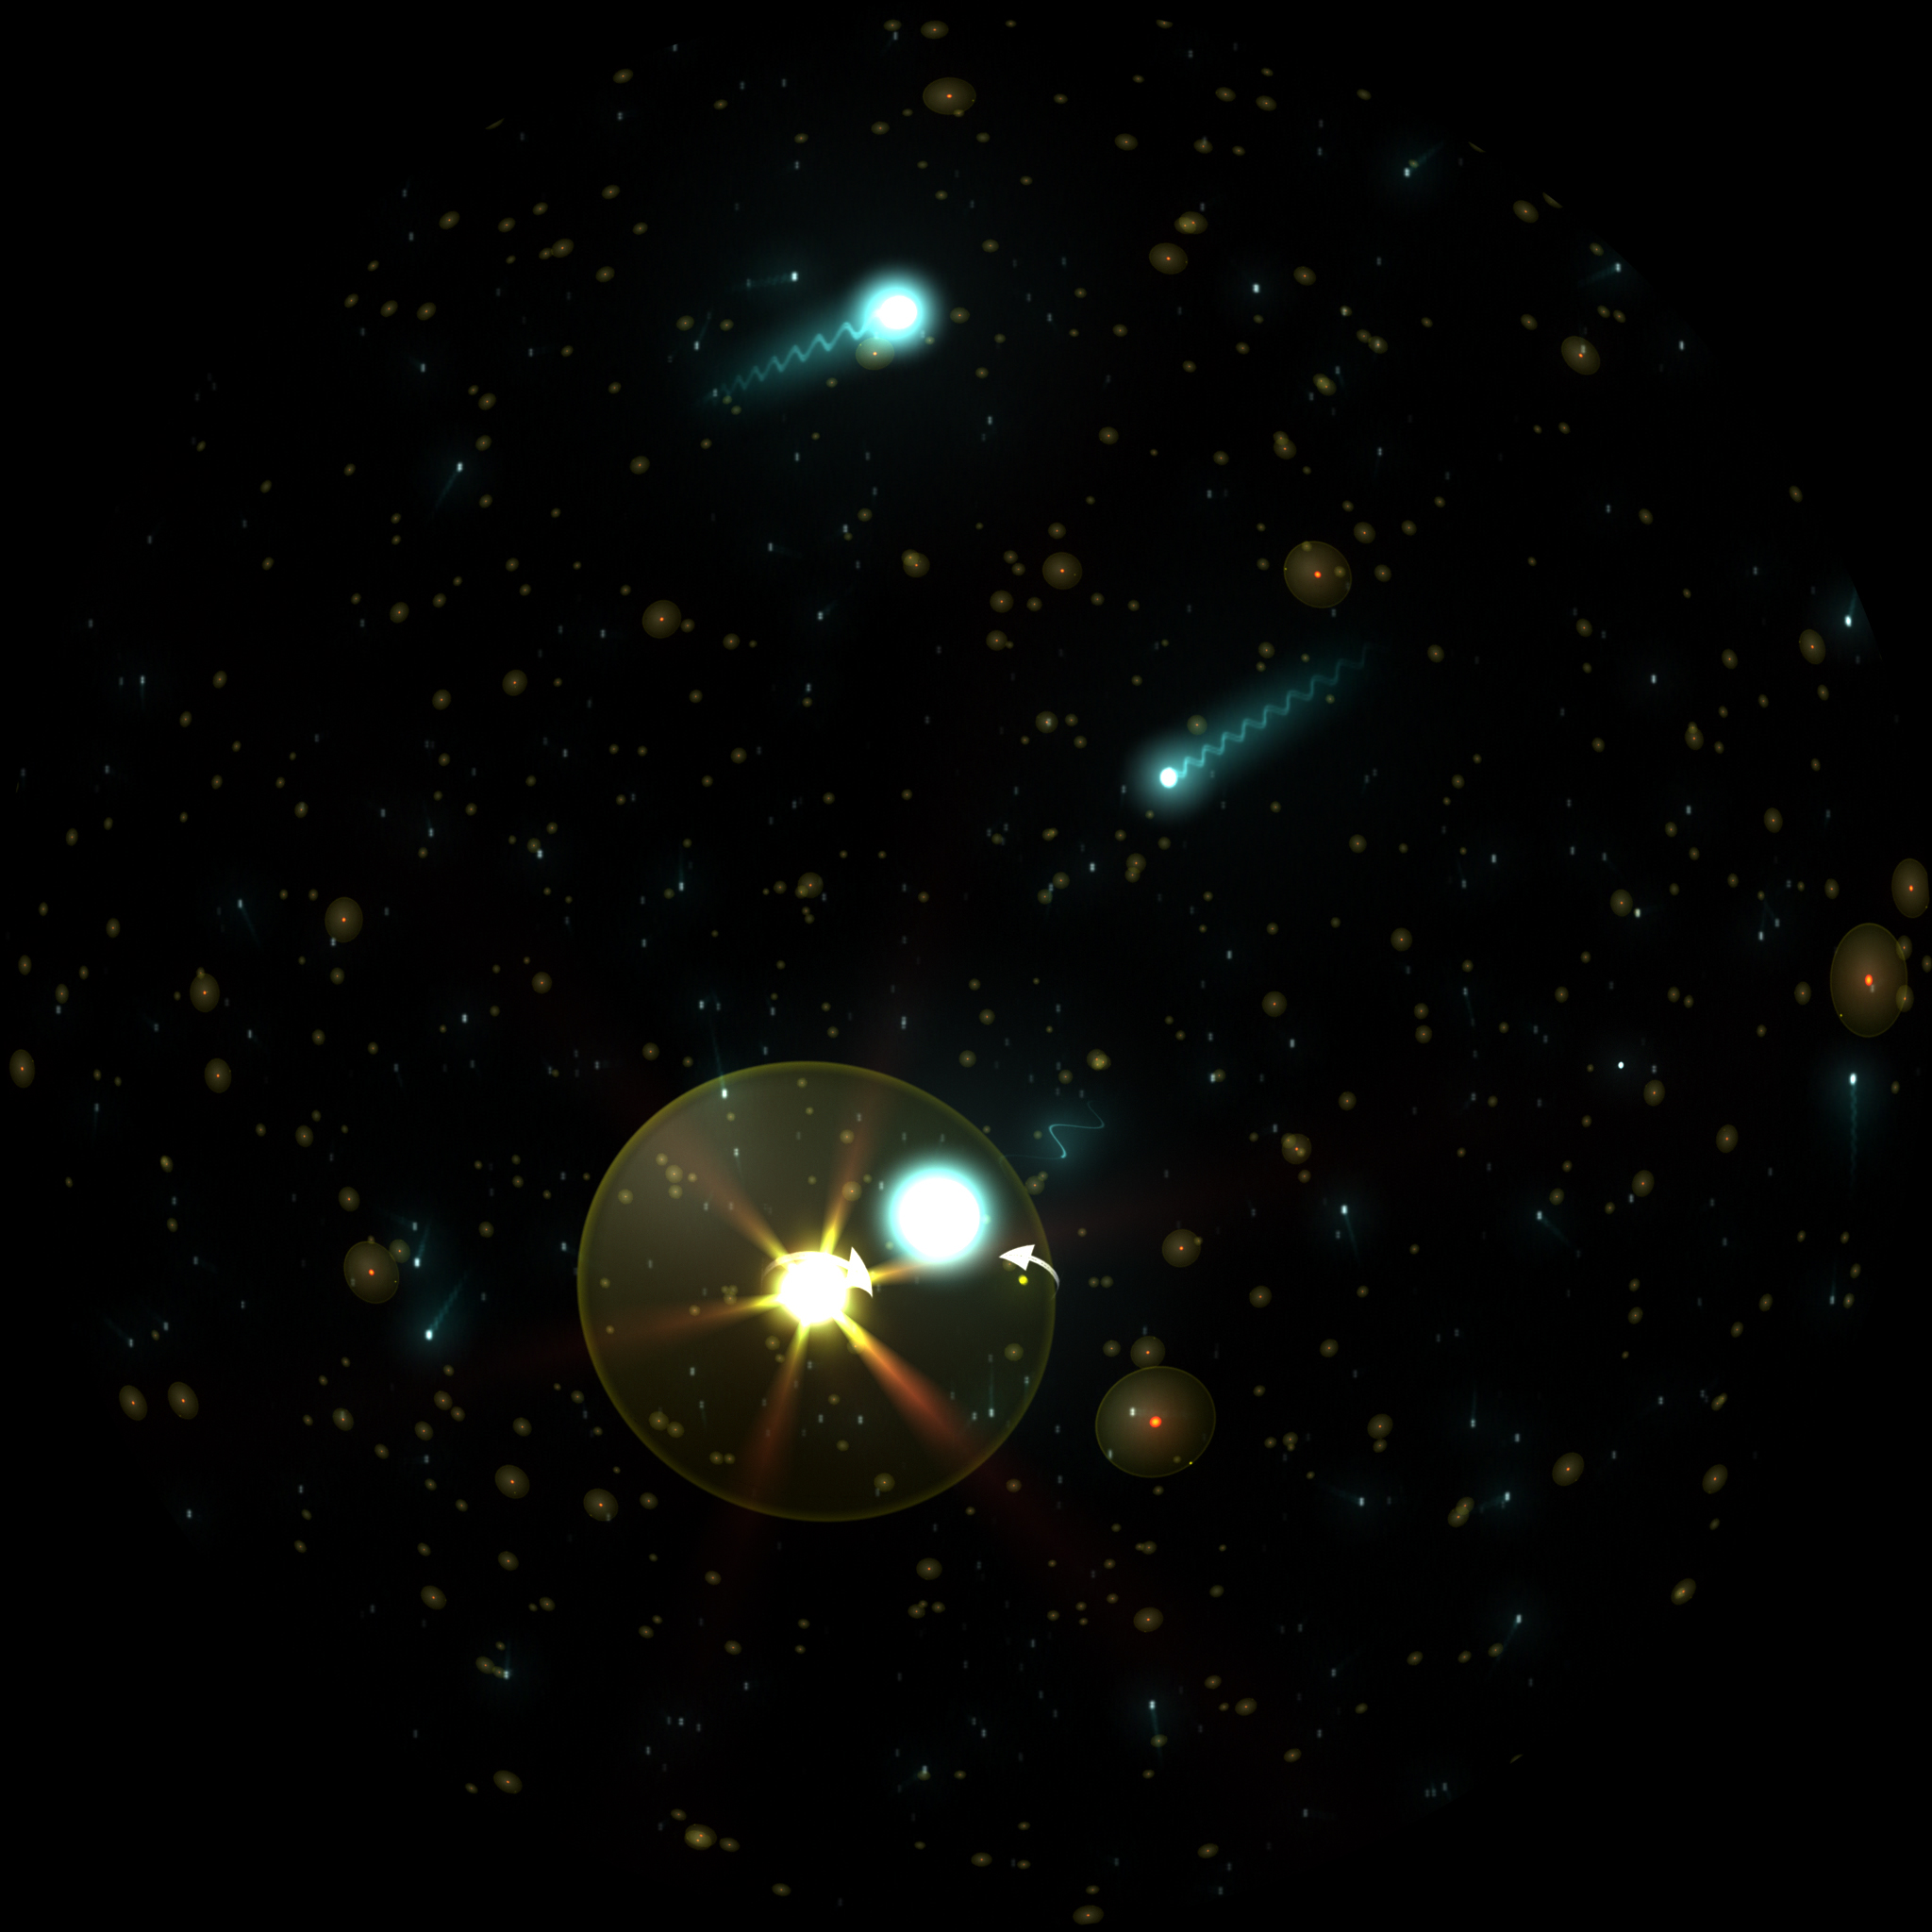
\includegraphics[width=0.3\textwidth]{Planetarium/figures/script_shots/shot12.jpg}} \vspace{0.1cm}\\

\hline

\textit{Because of this, when light passes through a Hydrogen gas cloud the number of 21 centimeter photons changes. }& 

\raisebox{-\totalheight}{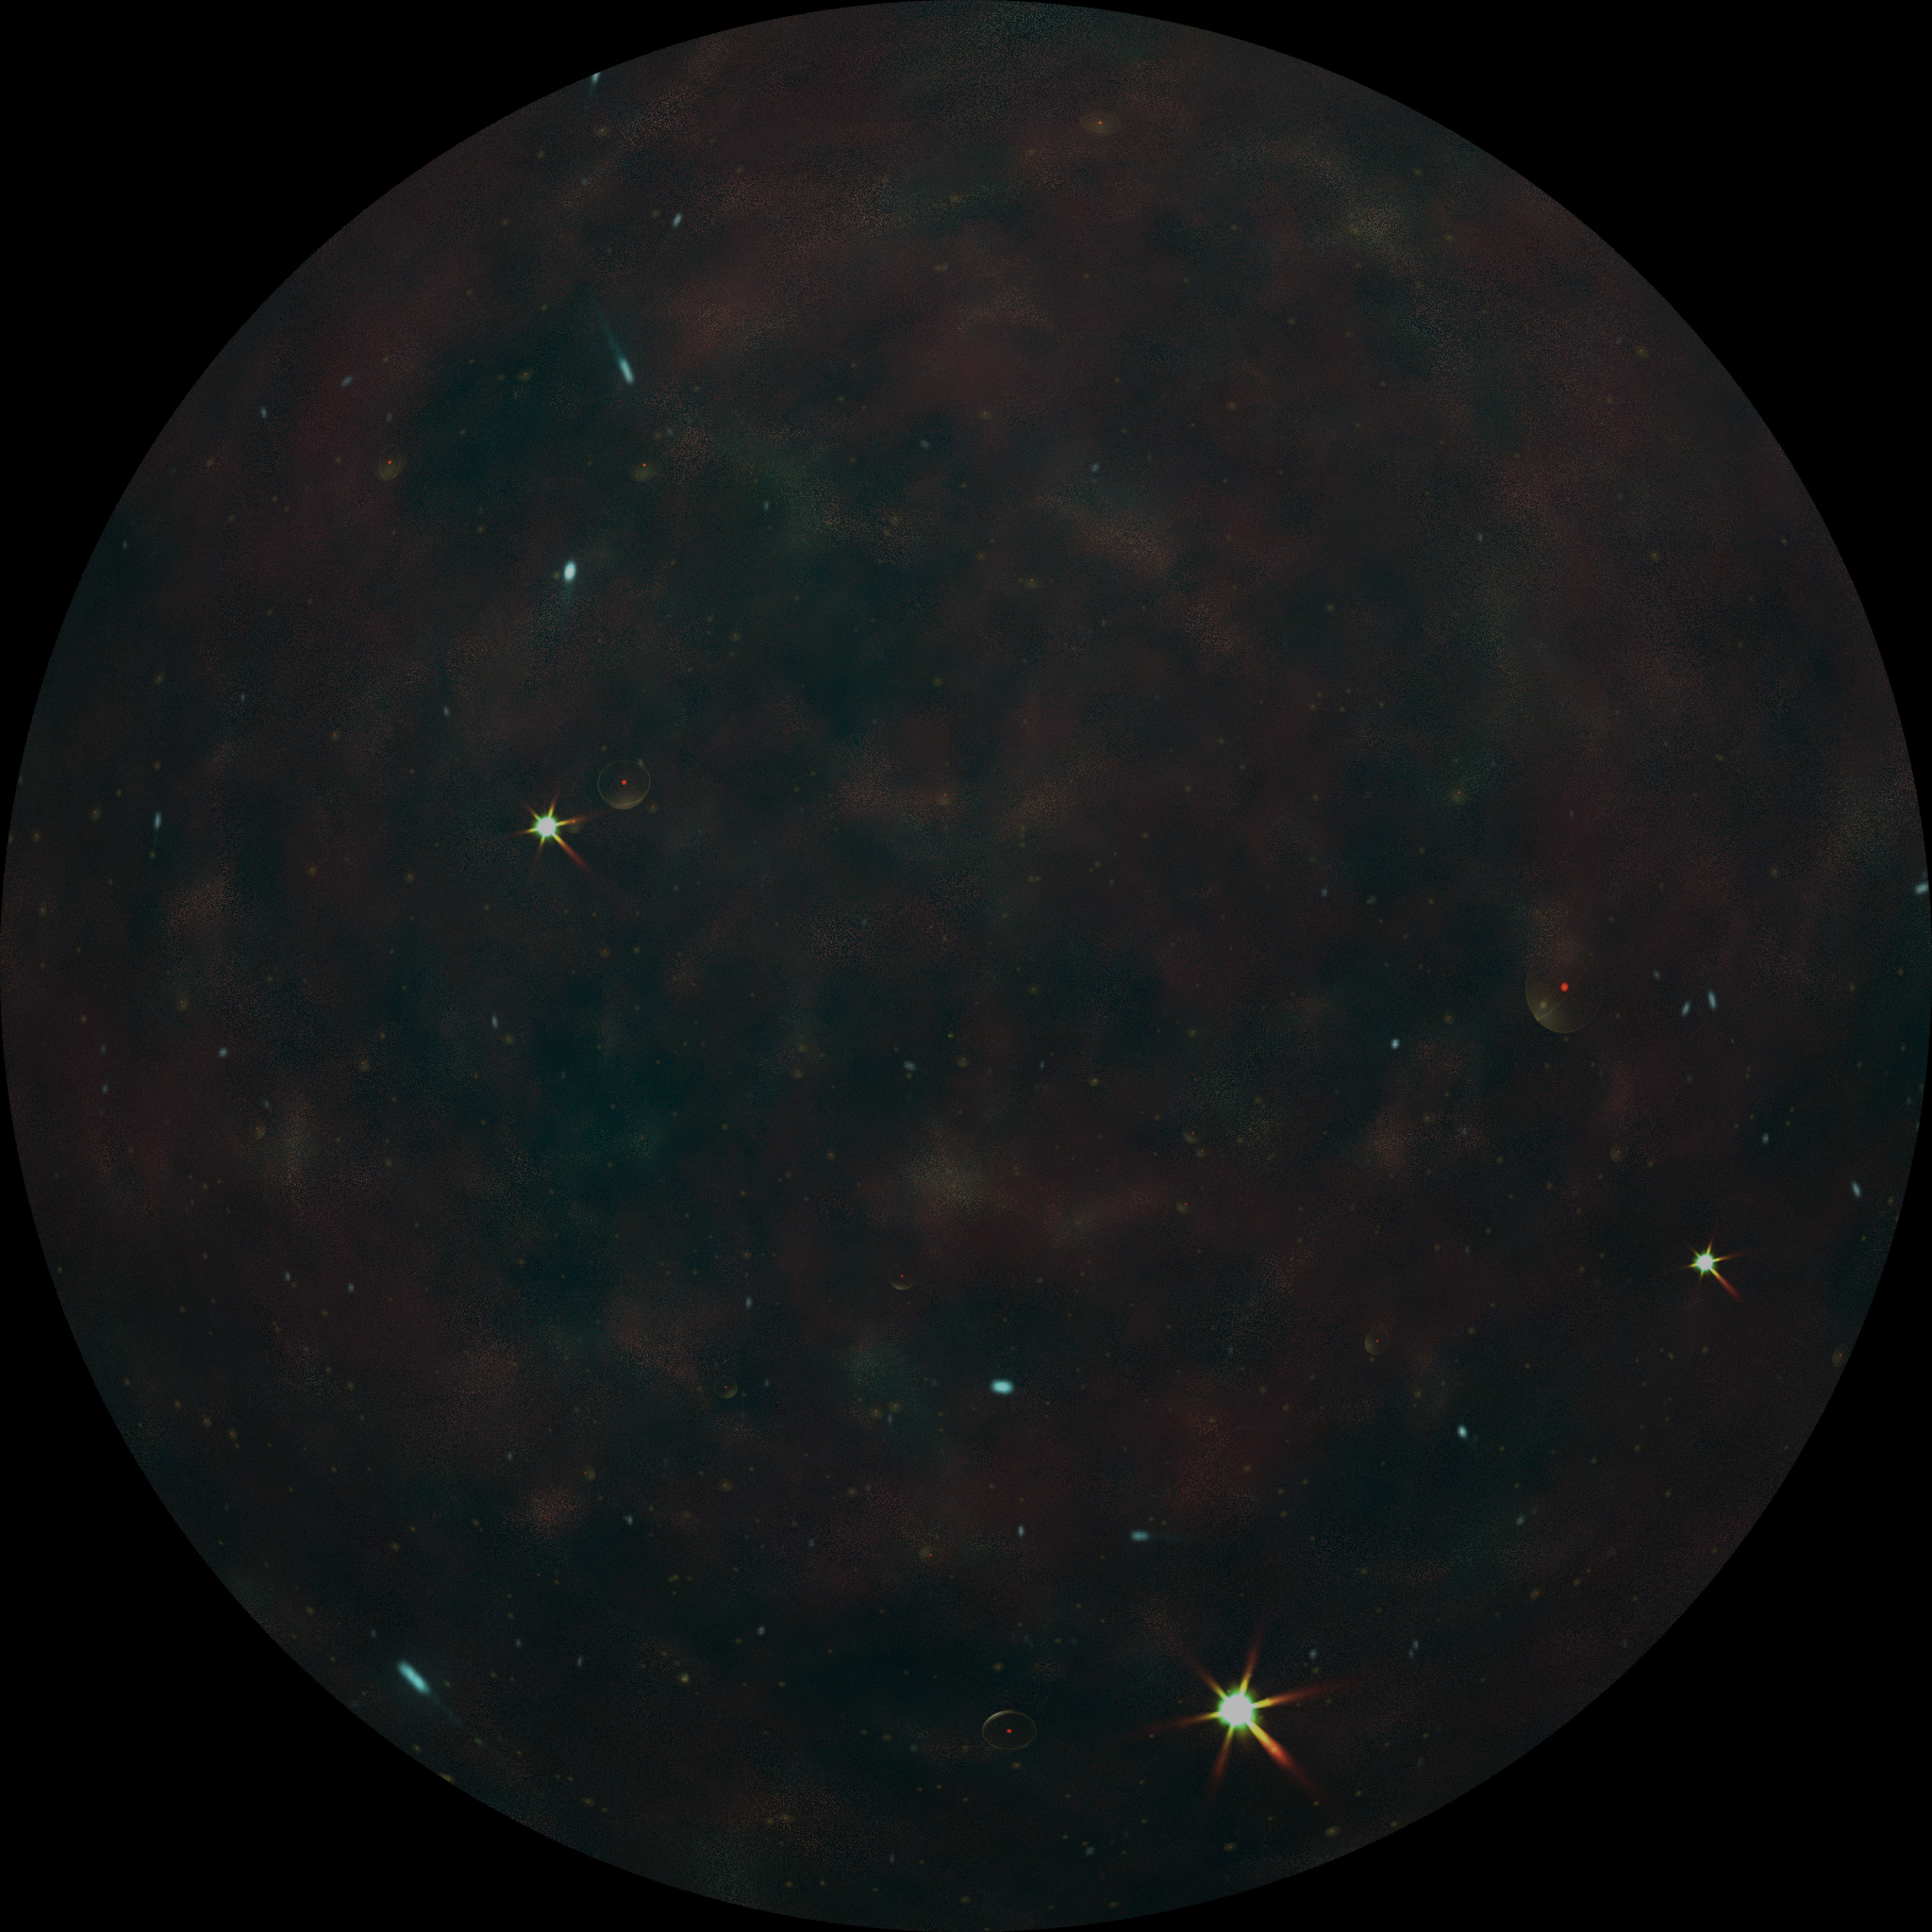
\includegraphics[width=0.3\textwidth]{Planetarium/figures/script_shots/shot13.jpg}} \vspace{0.1cm}\\

\hline

\textit{After passing through the Hydrogen gas cloud, the photons that remain continue to travel through the universe. As they travel, the universe expands around them. }& 

\raisebox{-\totalheight}{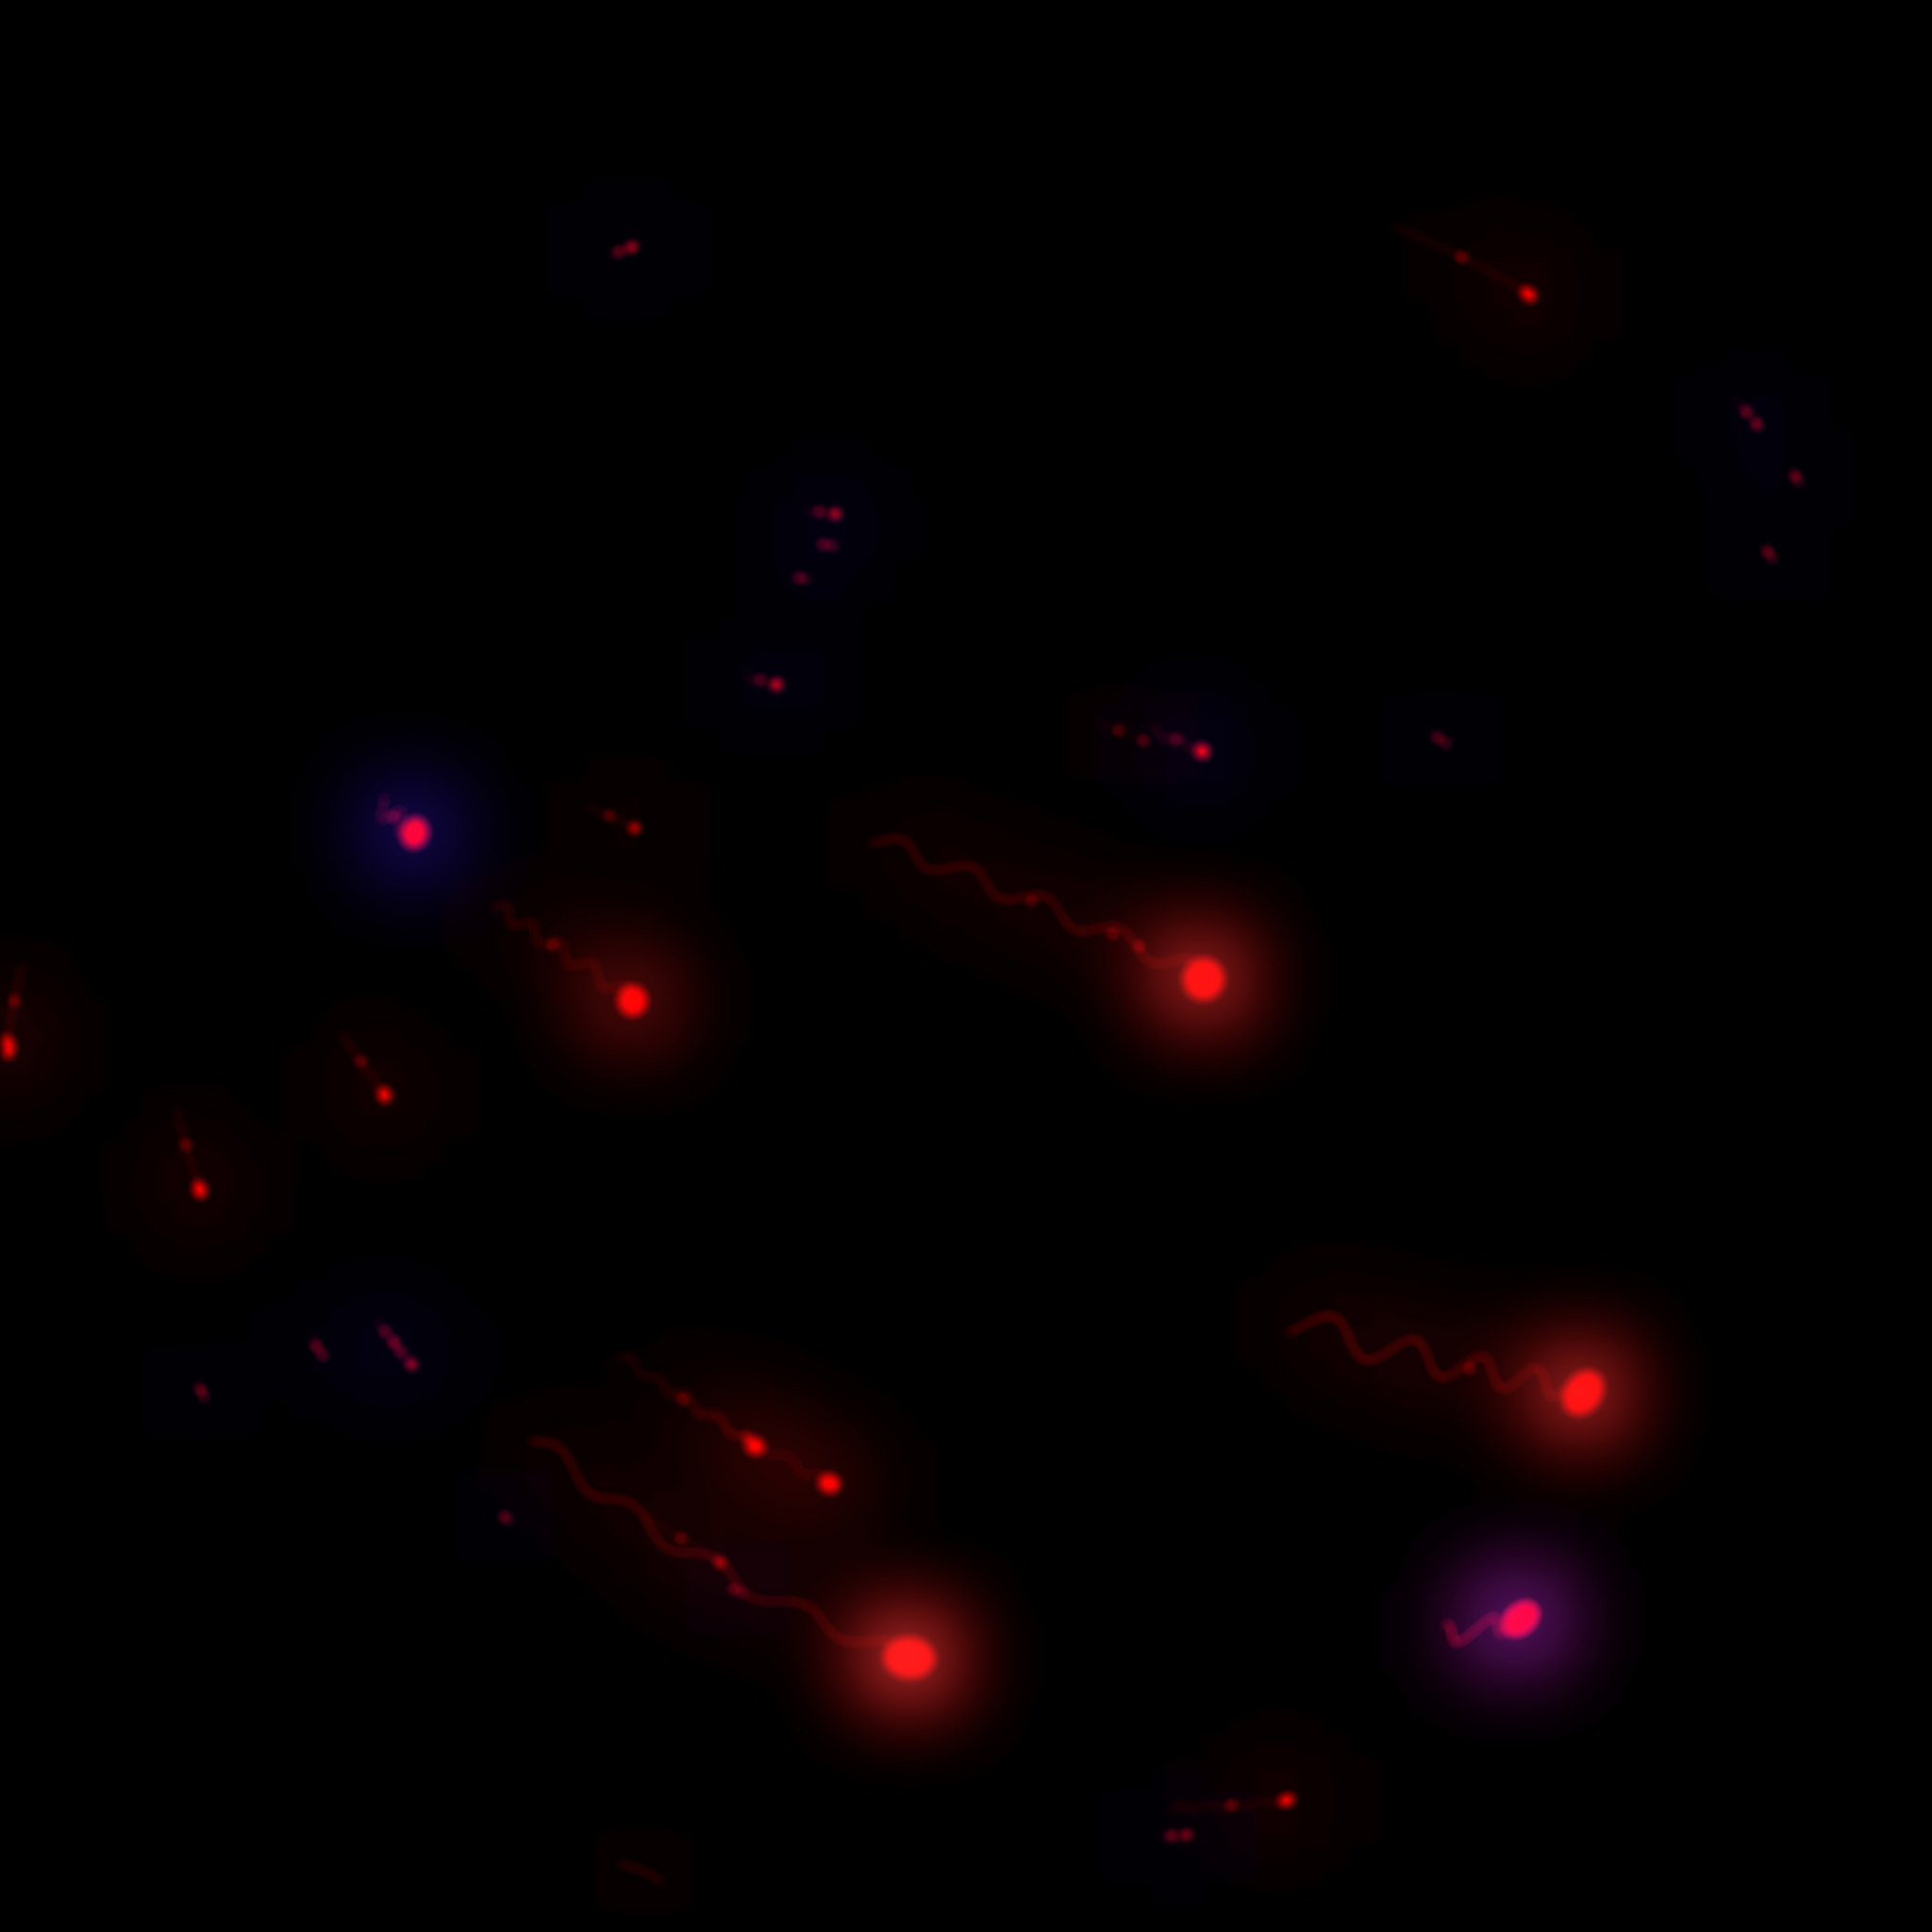
\includegraphics[width=0.3\textwidth]{Planetarium/figures/script_shots/shot14.jpg}} \vspace{0.1cm}\\

\hline

\textit{As the universe expands, or stretches, the wavelength of the photon also expands and grows longer.} &


 \raisebox{-\totalheight}{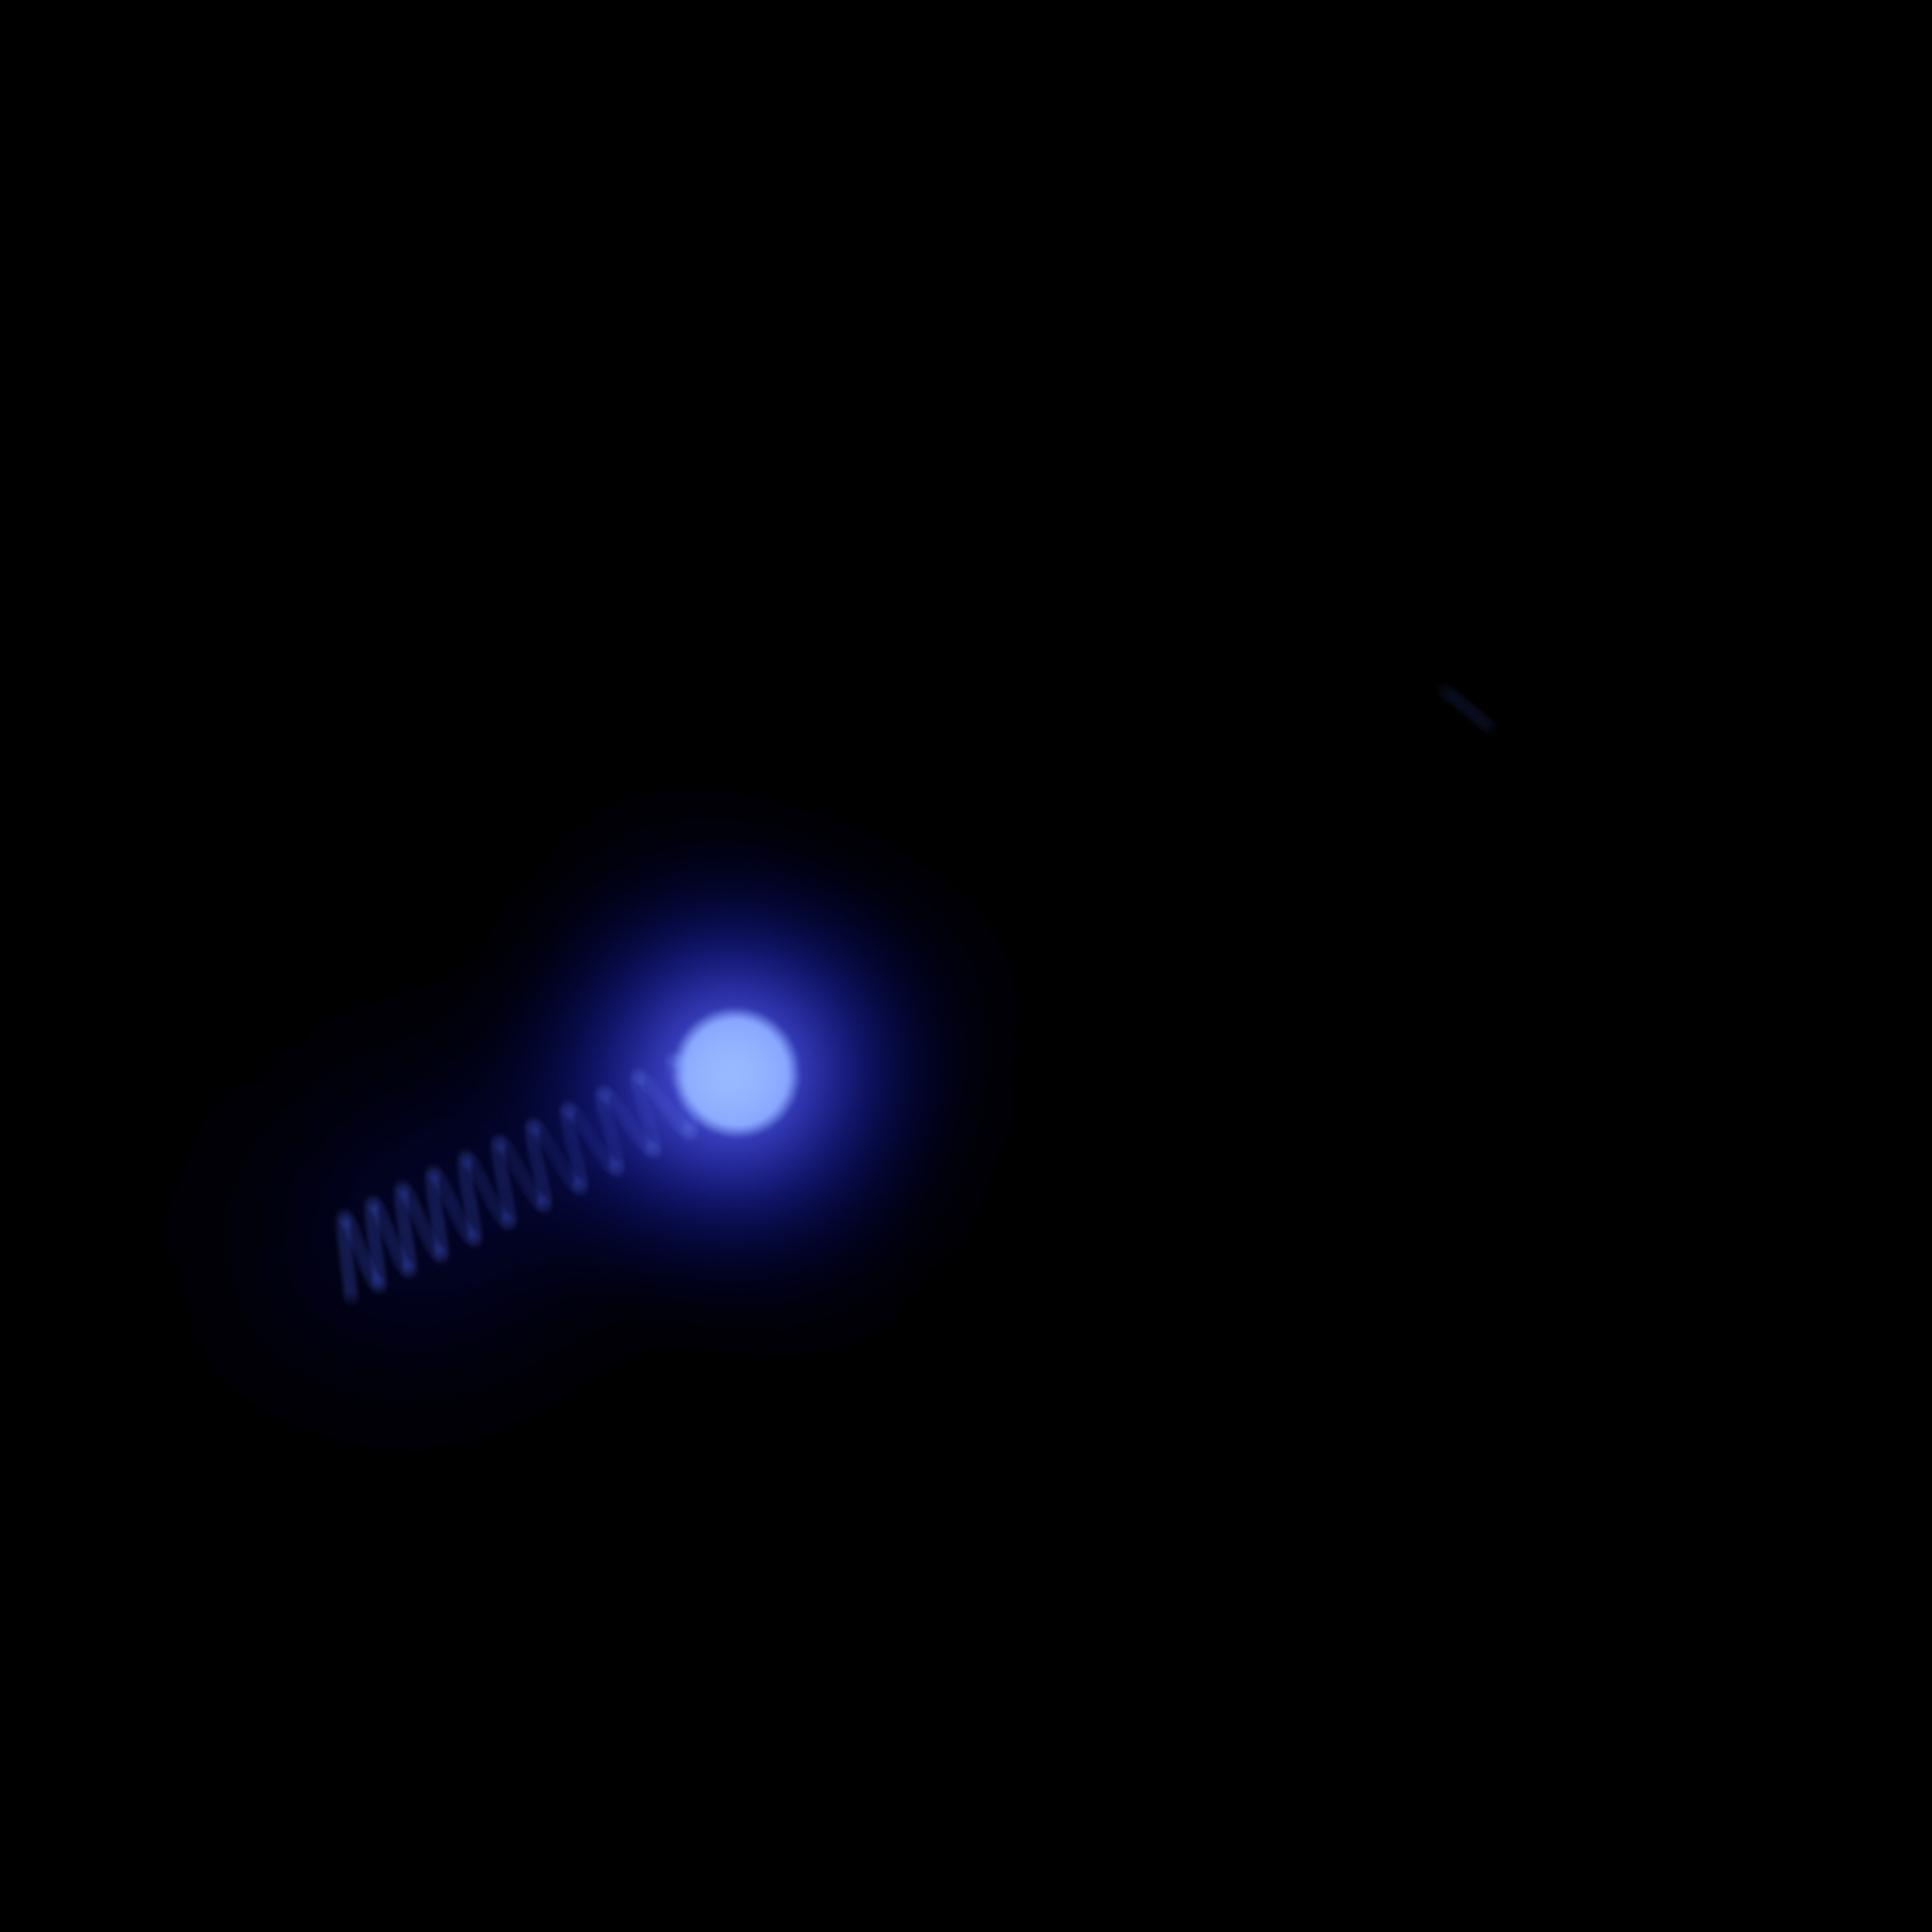
\includegraphics[width=0.3\textwidth]{Planetarium/figures/script_shots/shot15.jpg}} \vspace{0.1cm}\\

\hline

\textit{We call this expansion redshifting, because red light has longer wavelengths than blue light. }& 

\raisebox{-\totalheight}{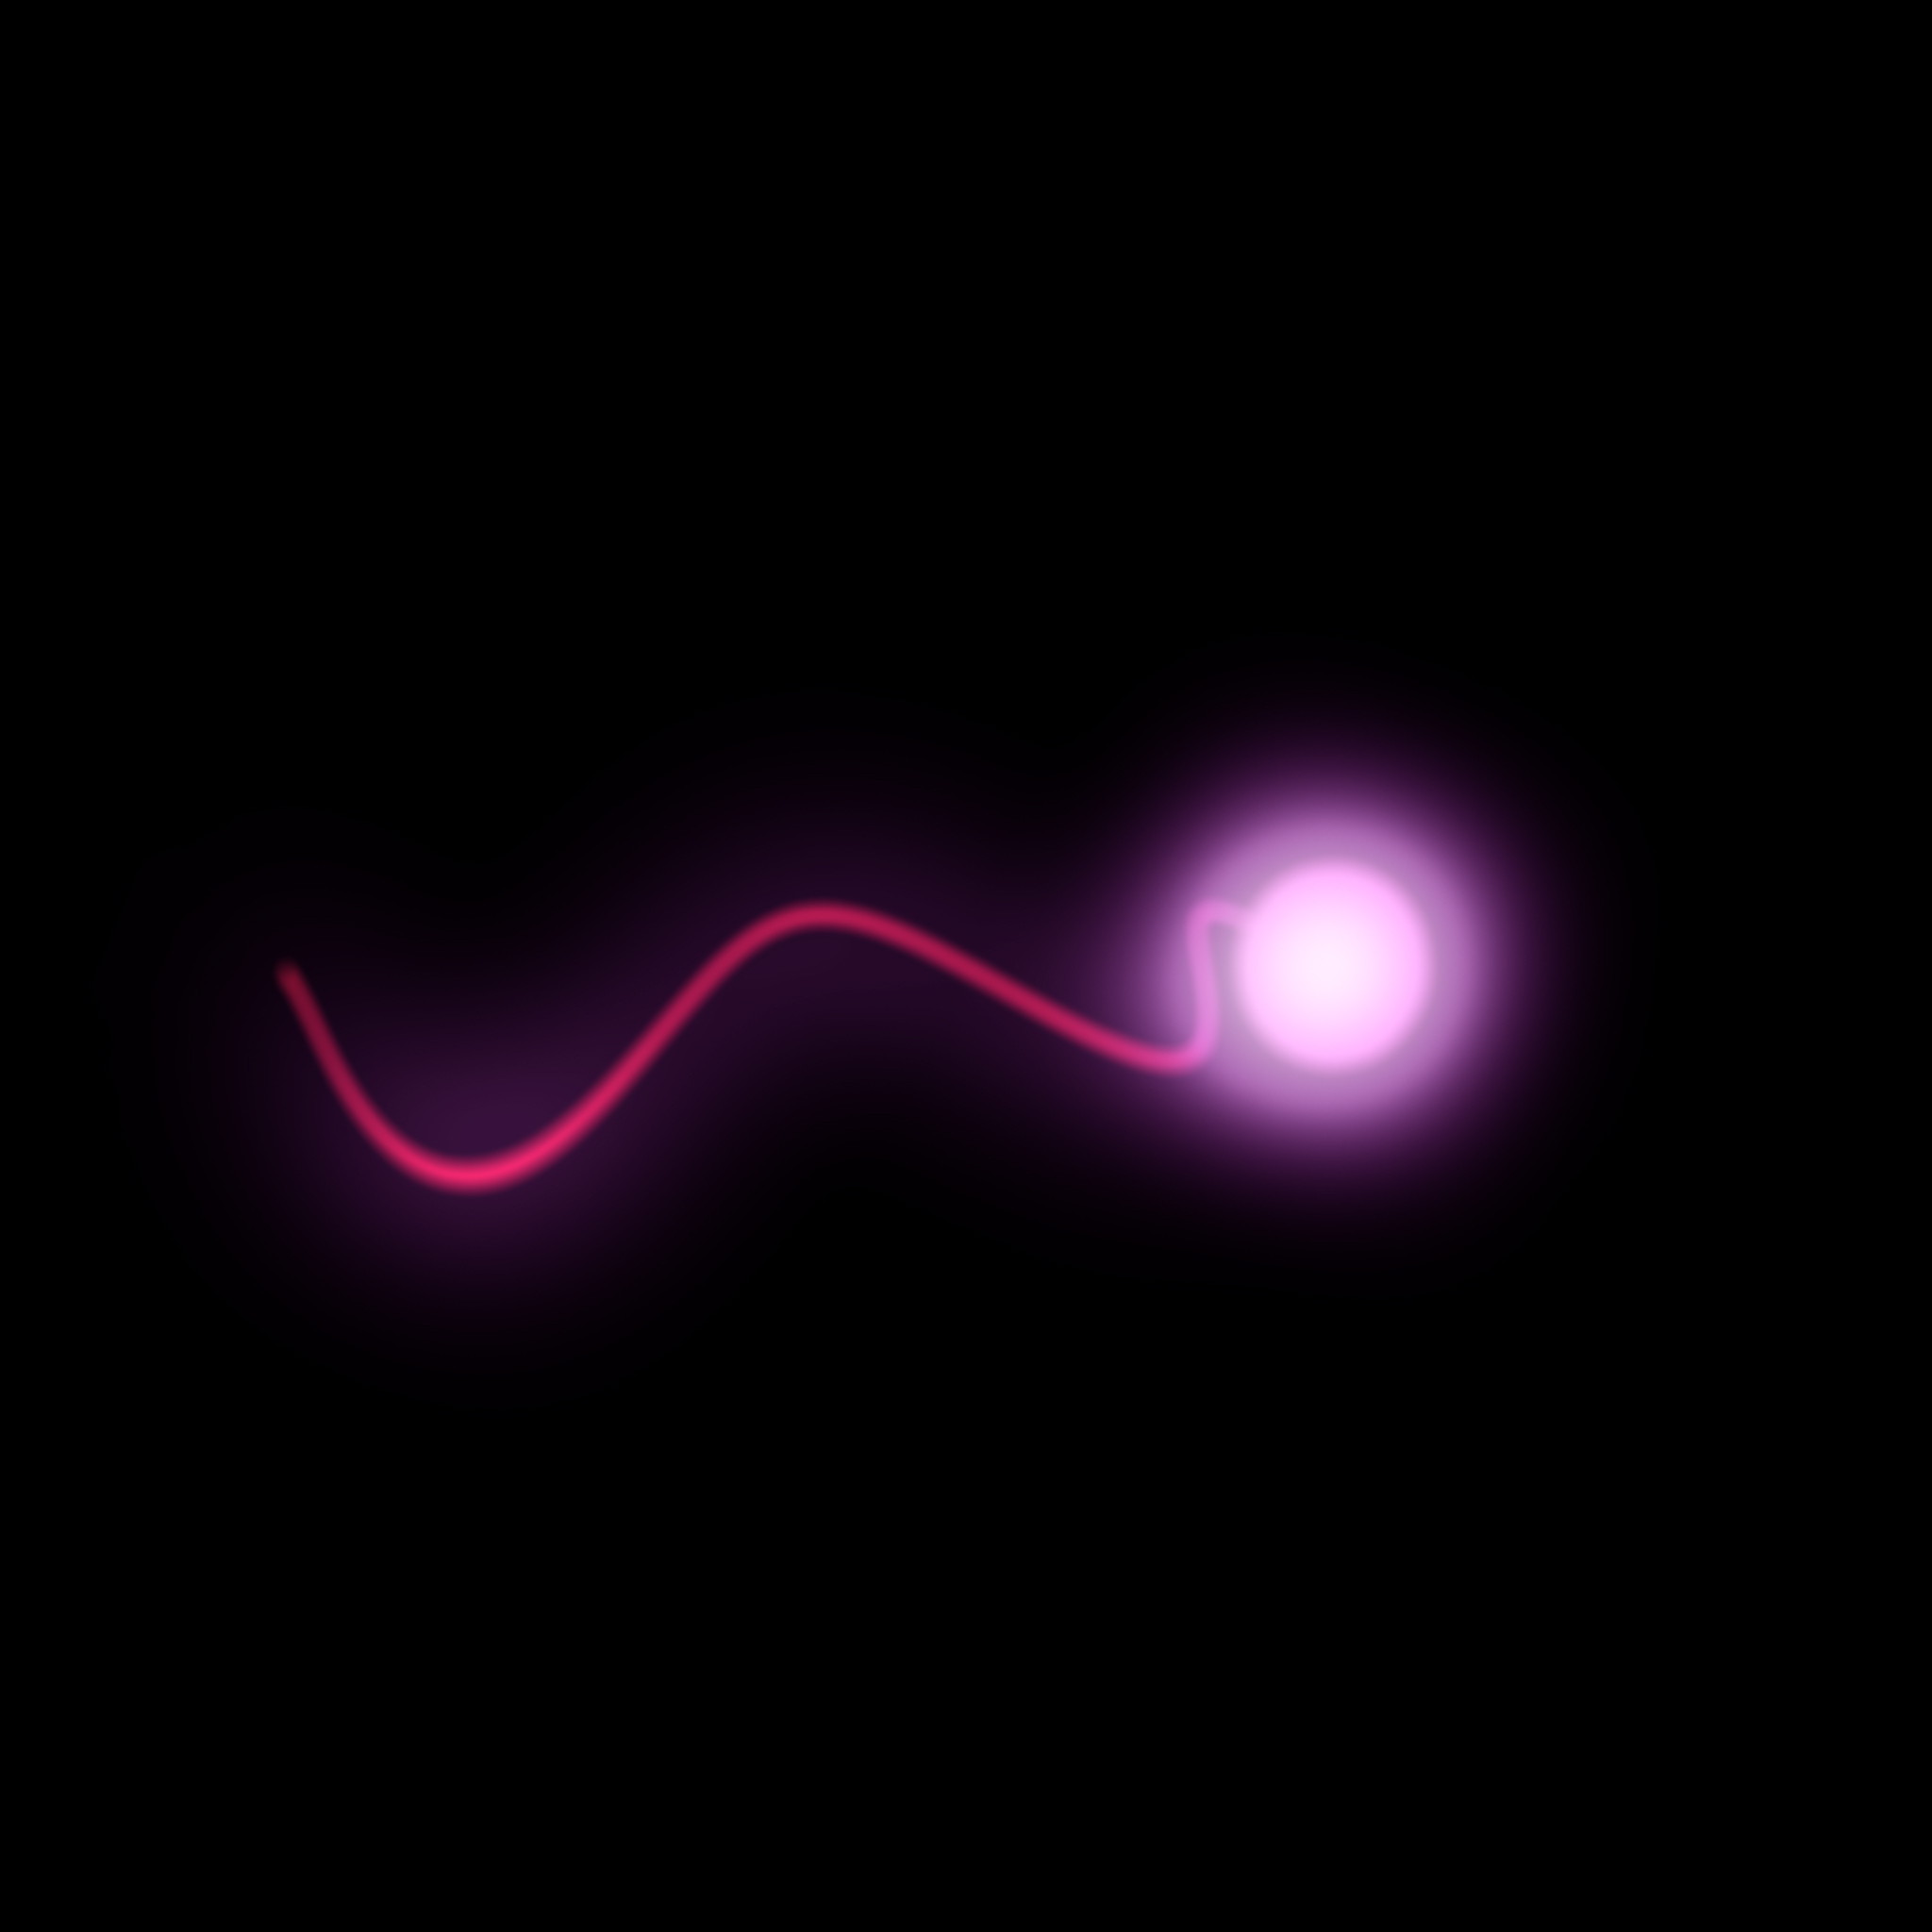
\includegraphics[width=0.3\textwidth]{Planetarium/figures/script_shots/shot16.jpg}} \vspace{0.1cm}\\

\hline

\textit{Eventually the photons reach the Milky Way Galaxy and approach the Earth, where they are measured by radio telescopes. }& 

\raisebox{-\totalheight}{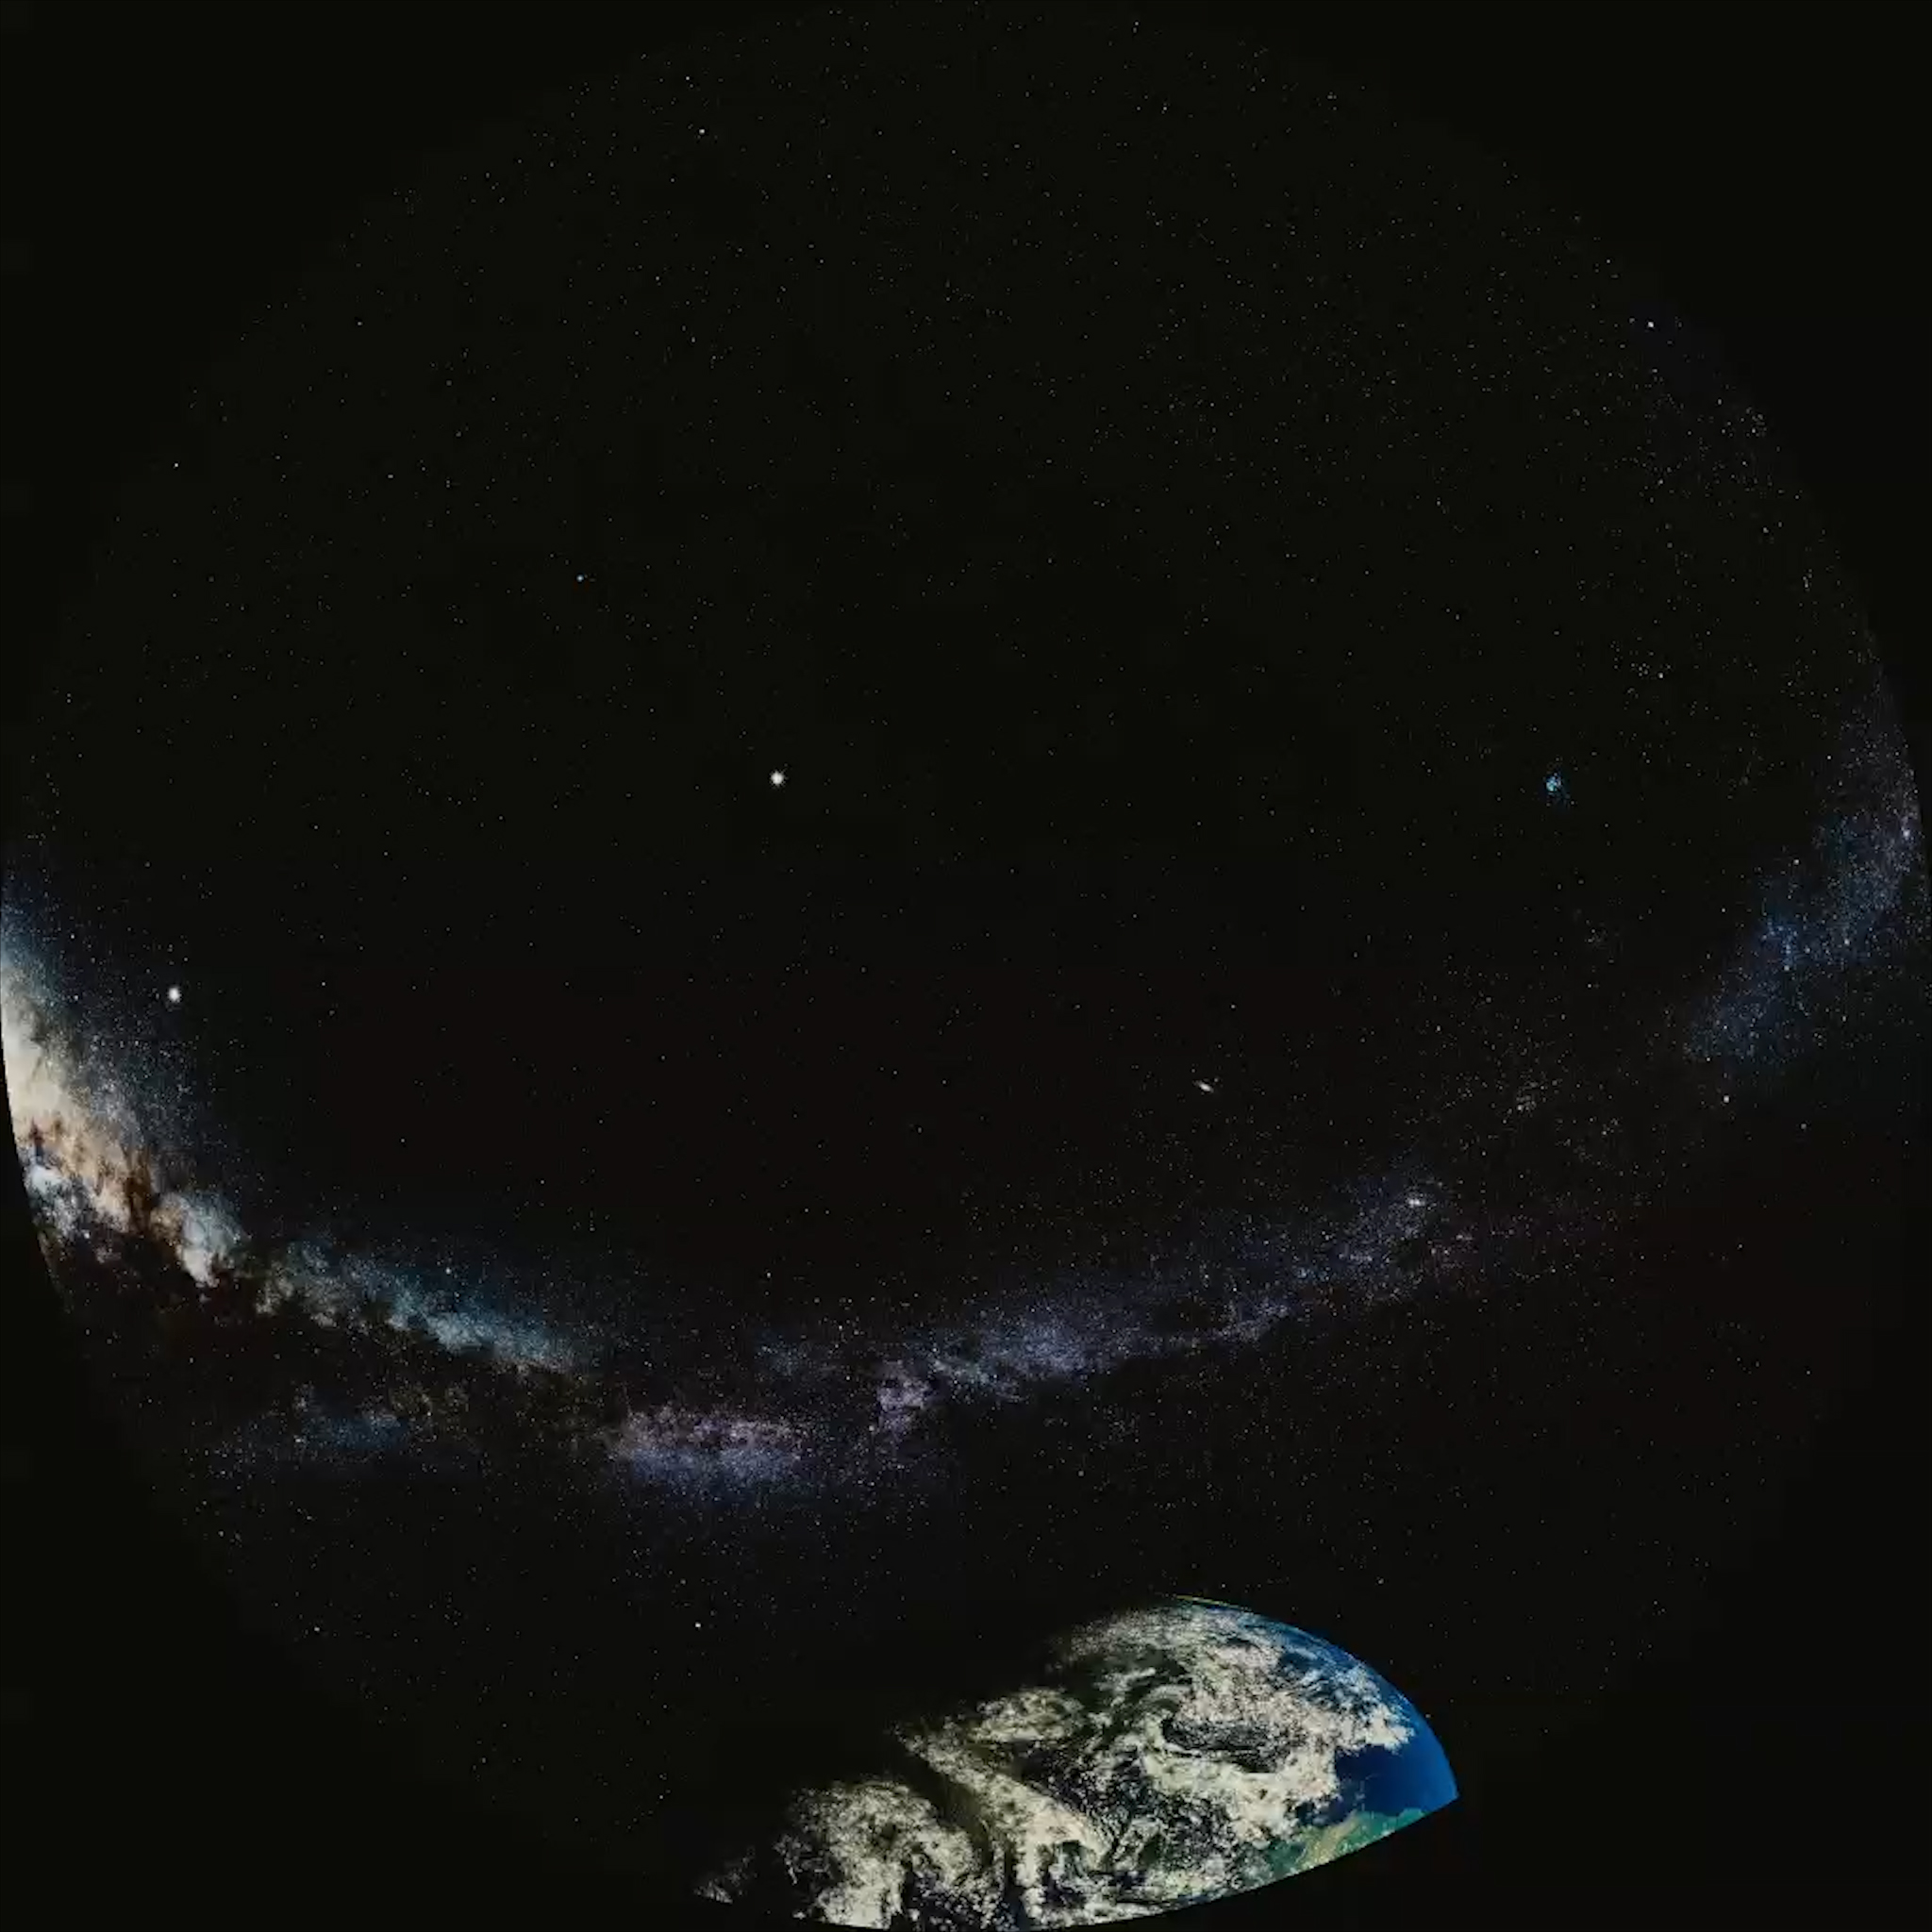
\includegraphics[width=0.3\textwidth]{Planetarium/figures/script_shots/shot17.jpg}}\vspace{0.1cm}\\ 

\hline

\textit{One such radio telescope is the Robert C. Byrd Green Bank Radio Telescope in southern West Virginia.  }& 

\raisebox{-\totalheight}{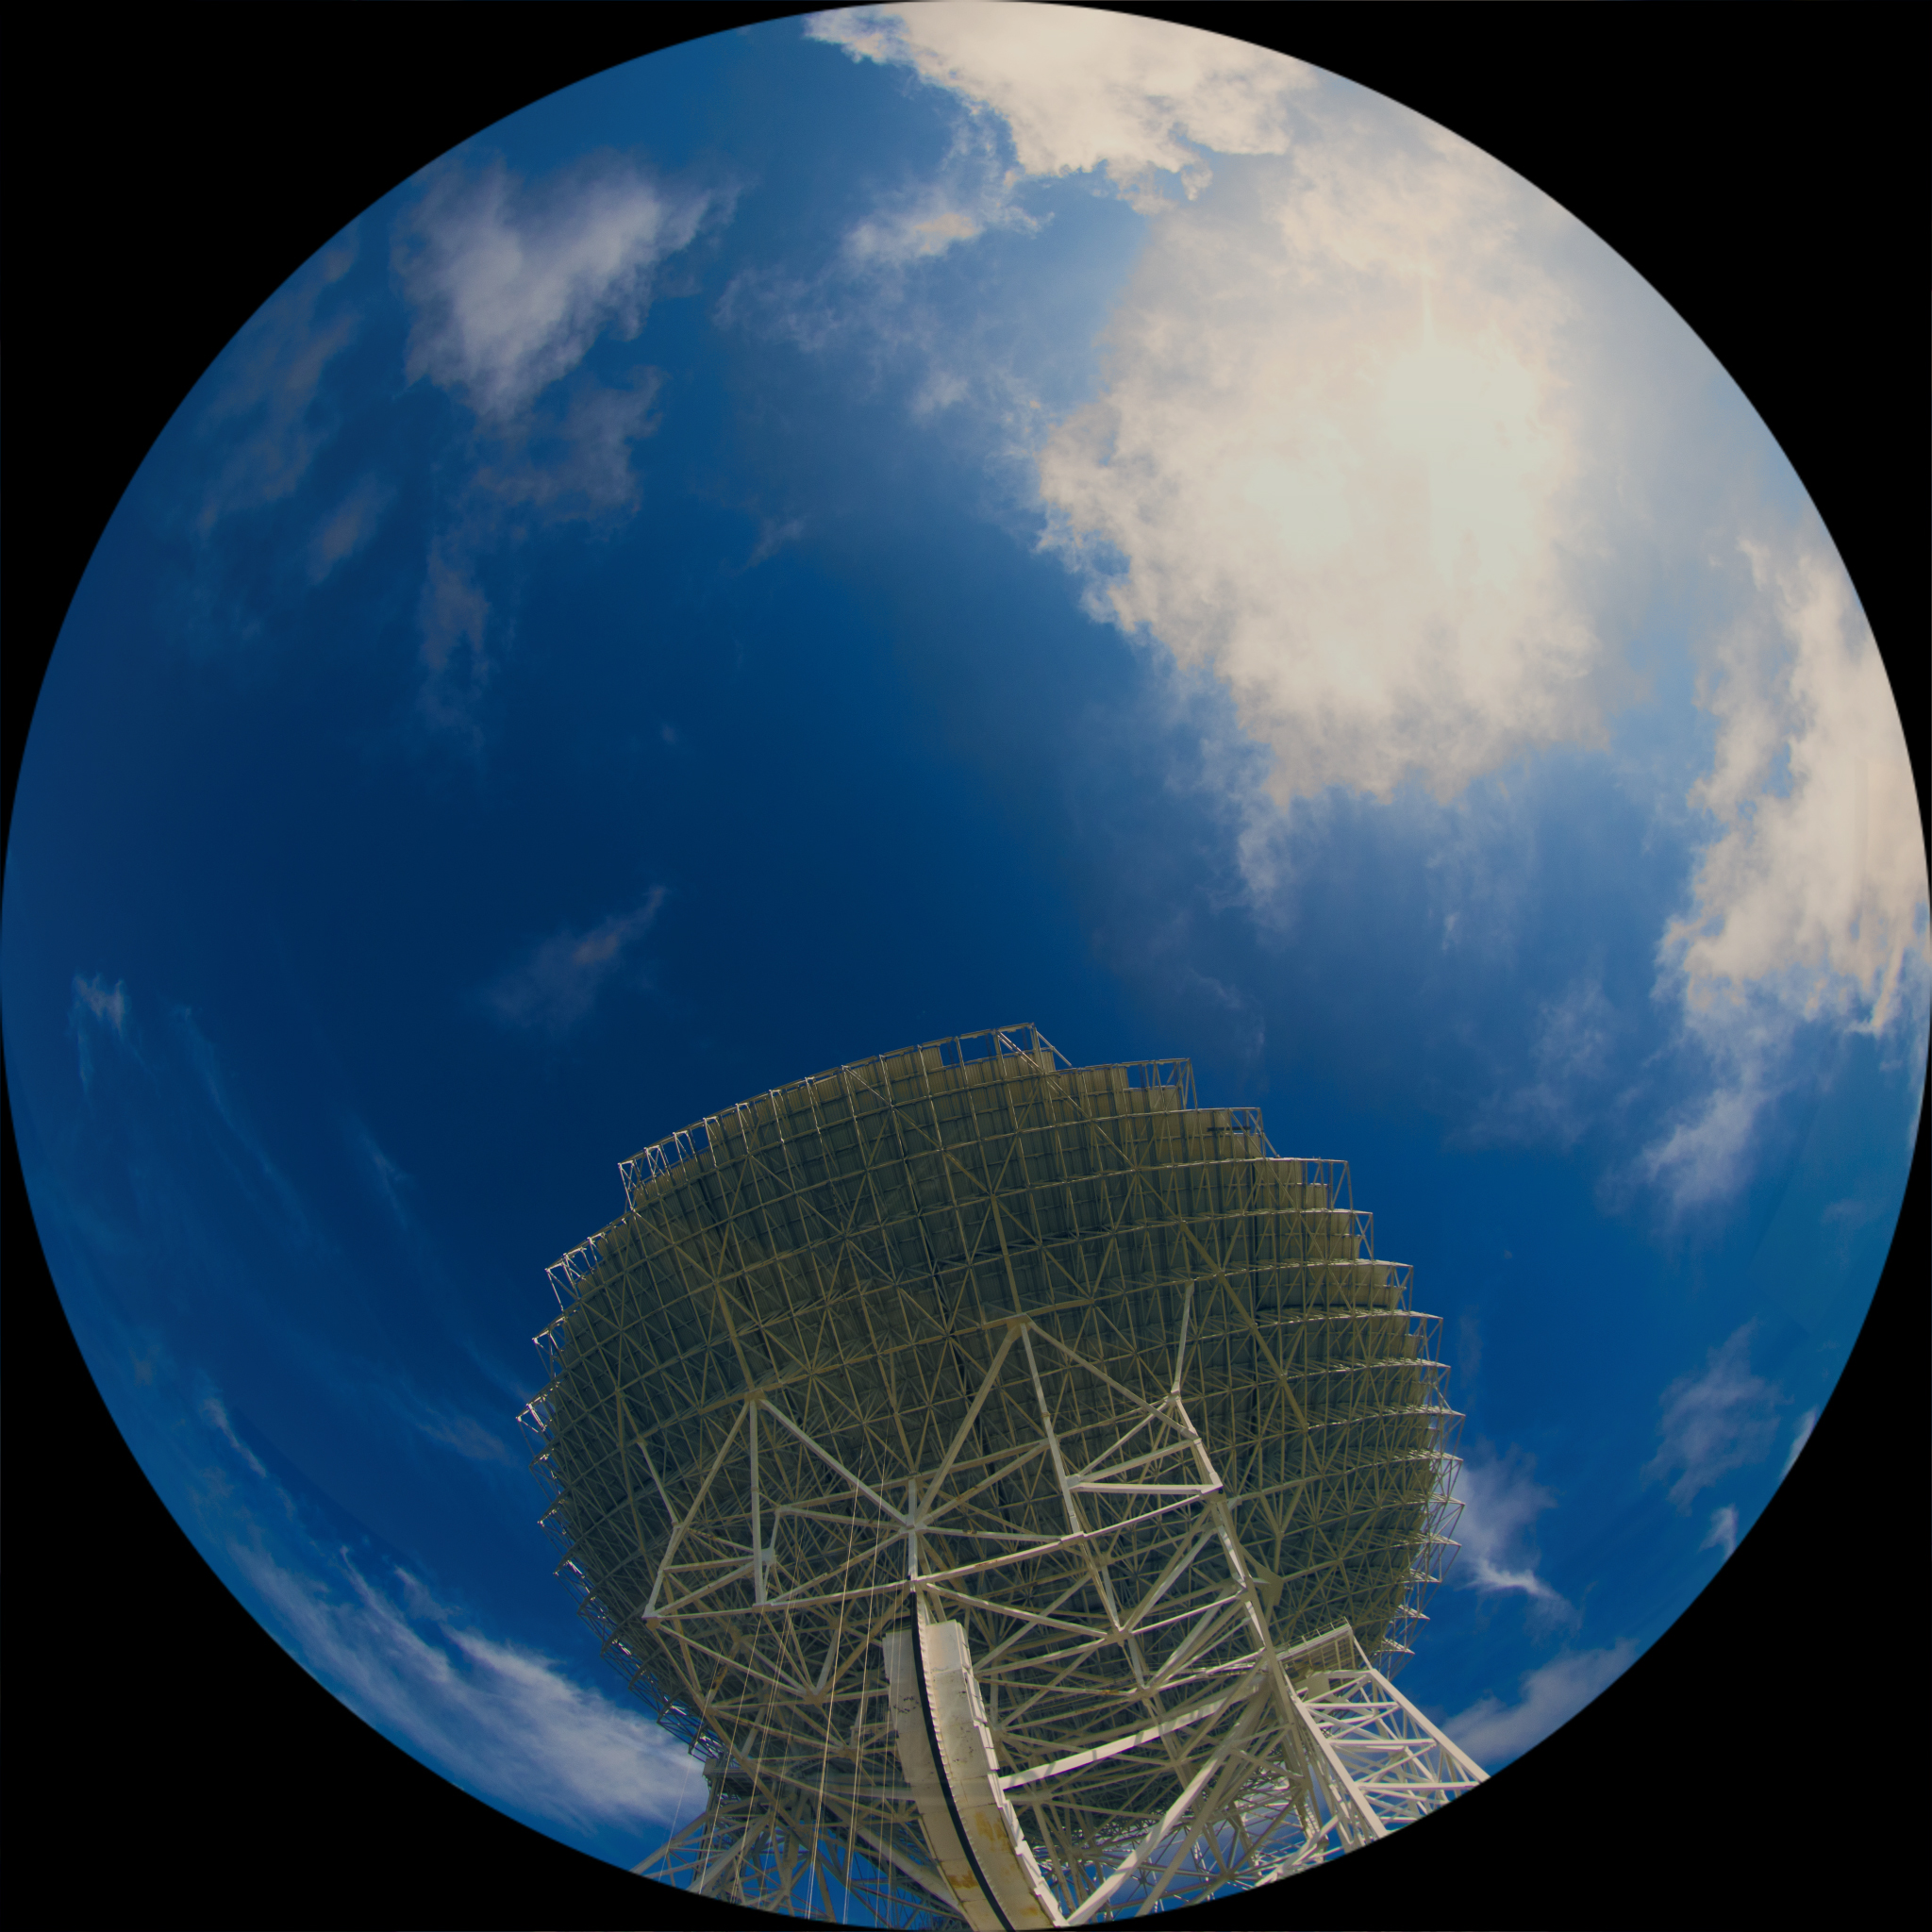
\includegraphics[width=0.3\textwidth]{Planetarium/figures/script_shots/shot18.jpg}} \vspace{0.1cm}\\

\hline

\textit{At the Green Bank Telescope, light is captured by a receiver located above the huge dish of the telescope. }& 

\raisebox{-\totalheight}{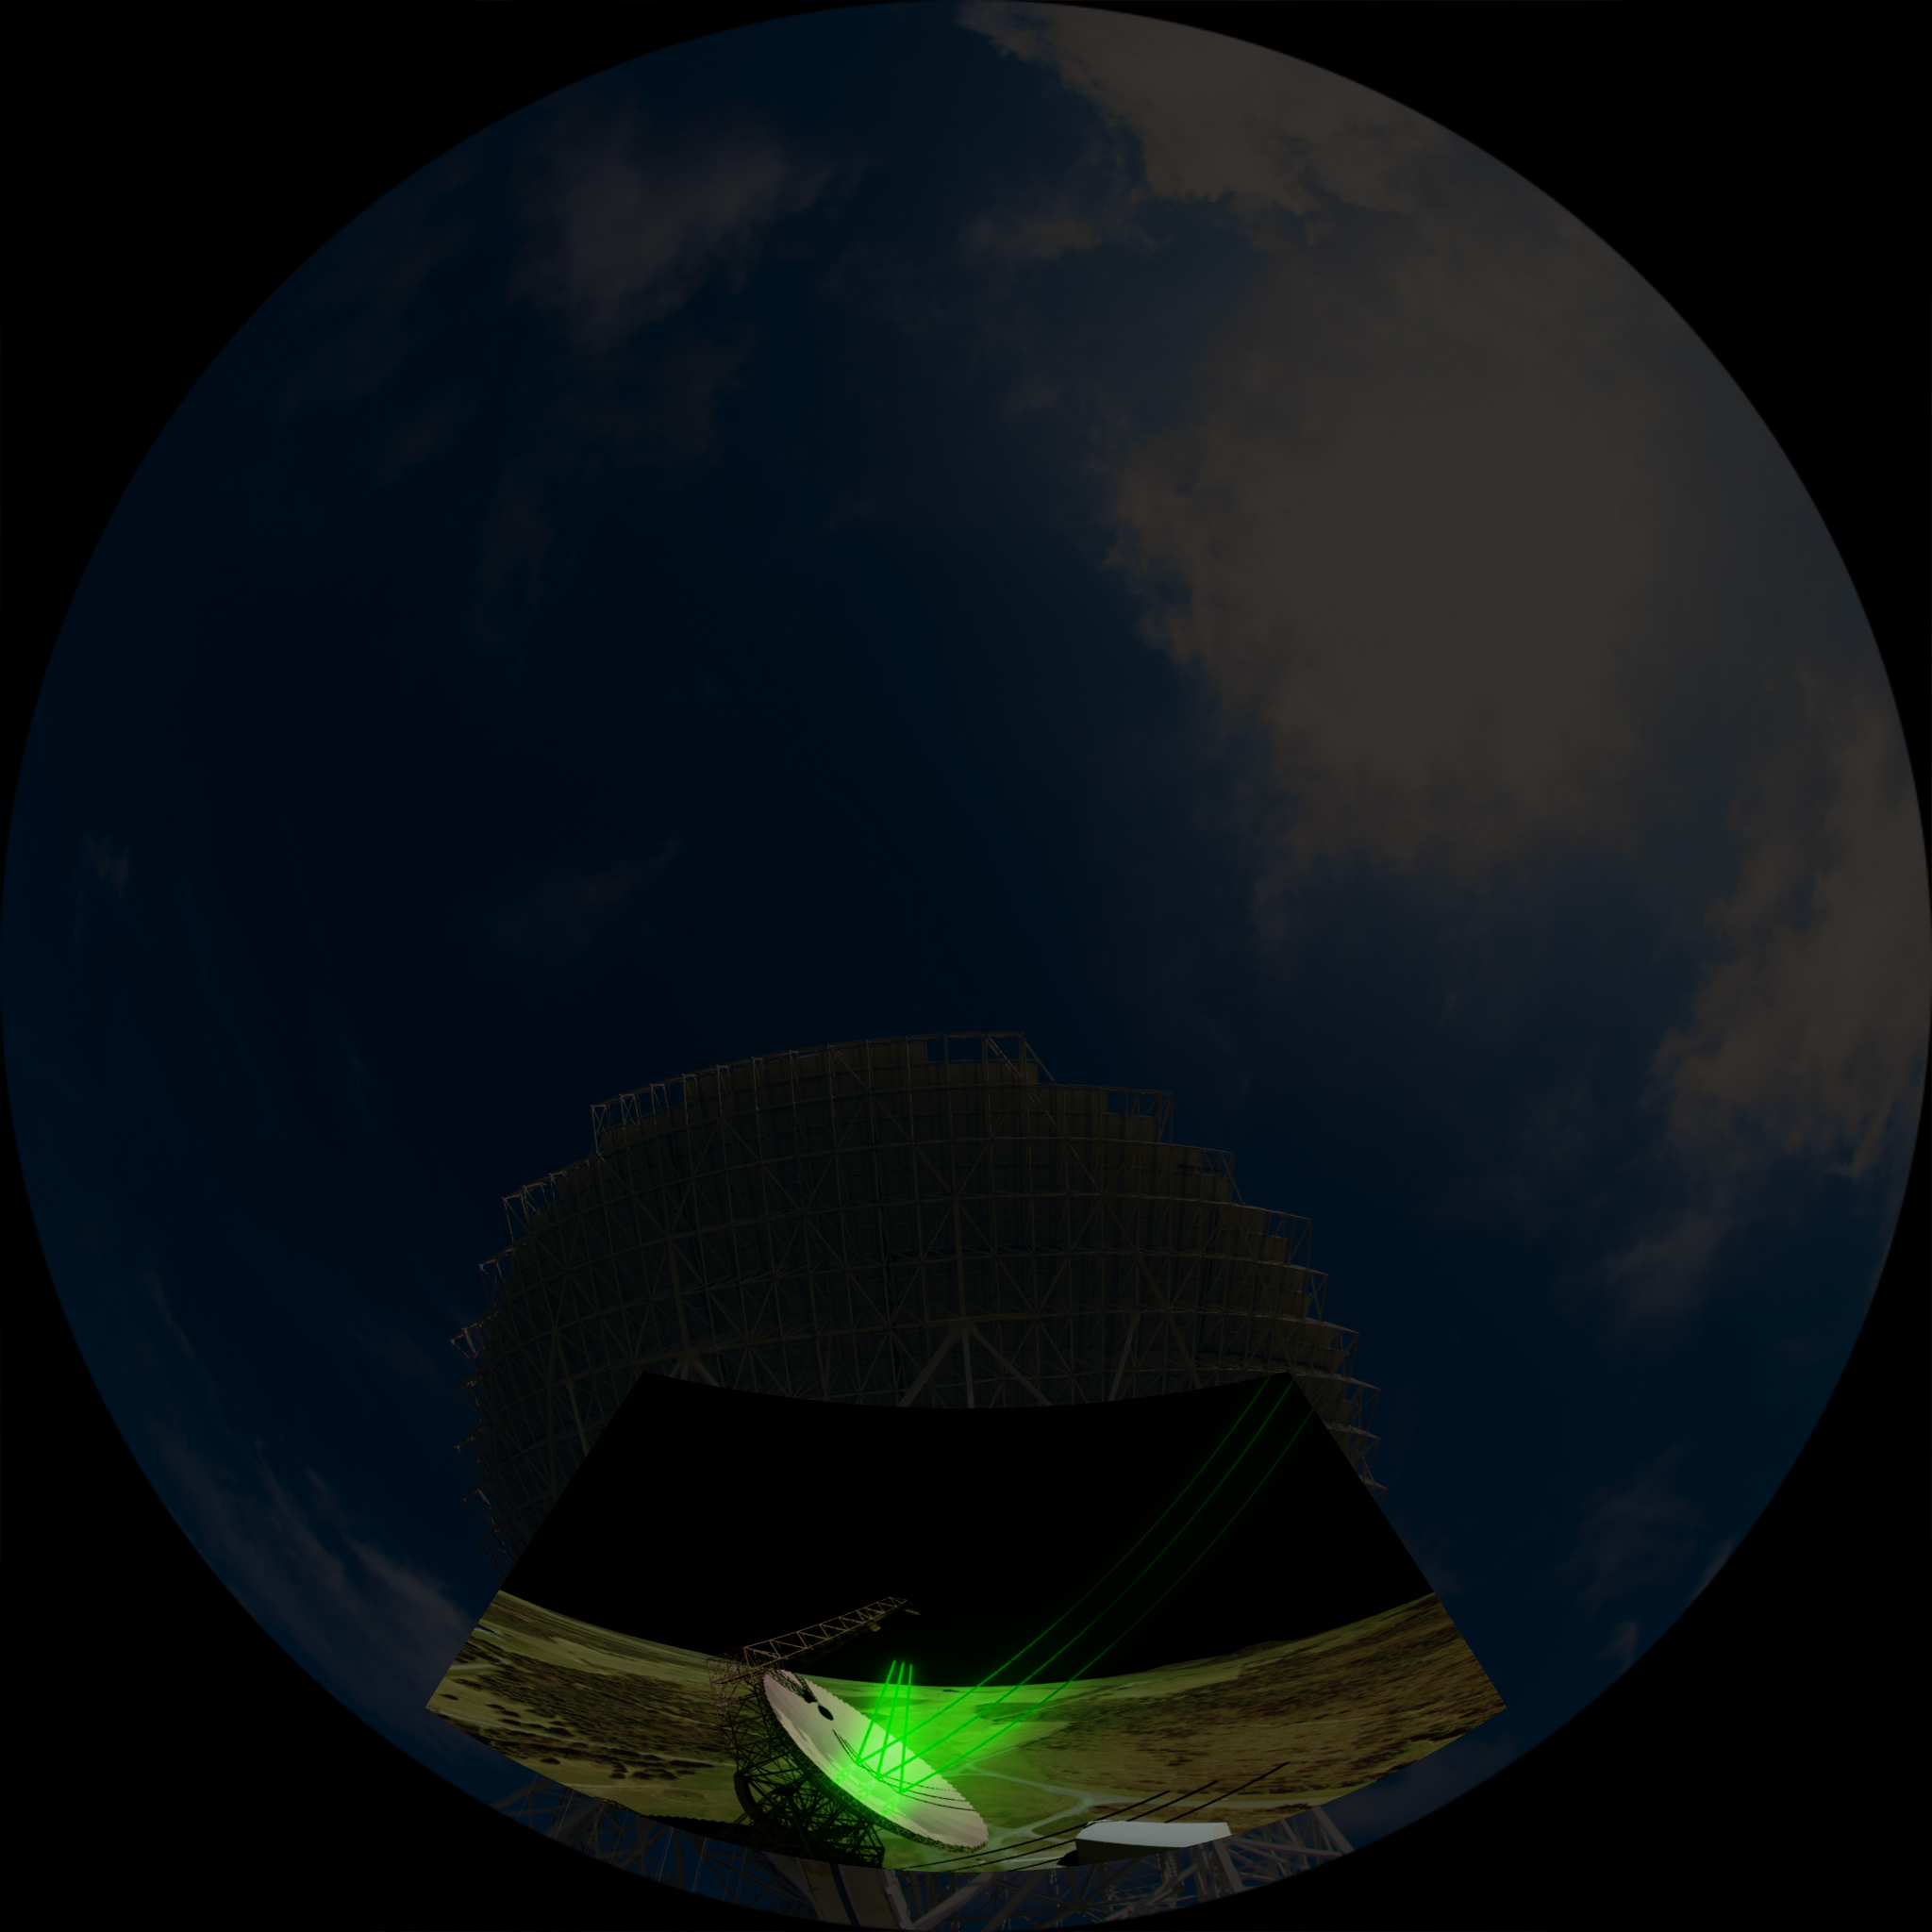
\includegraphics[width=0.3\textwidth]{Planetarium/figures/script_shots/shot19.jpg}} \vspace{0.1cm}\\

\hline

\textit{From there it is sent down along cables into nearby computers. Once inside the computers, the light is chopped up in time, and then further separated into groups by wavelength. In this way, we can measure a spectrum of light at each second. }& 

\raisebox{-\totalheight}{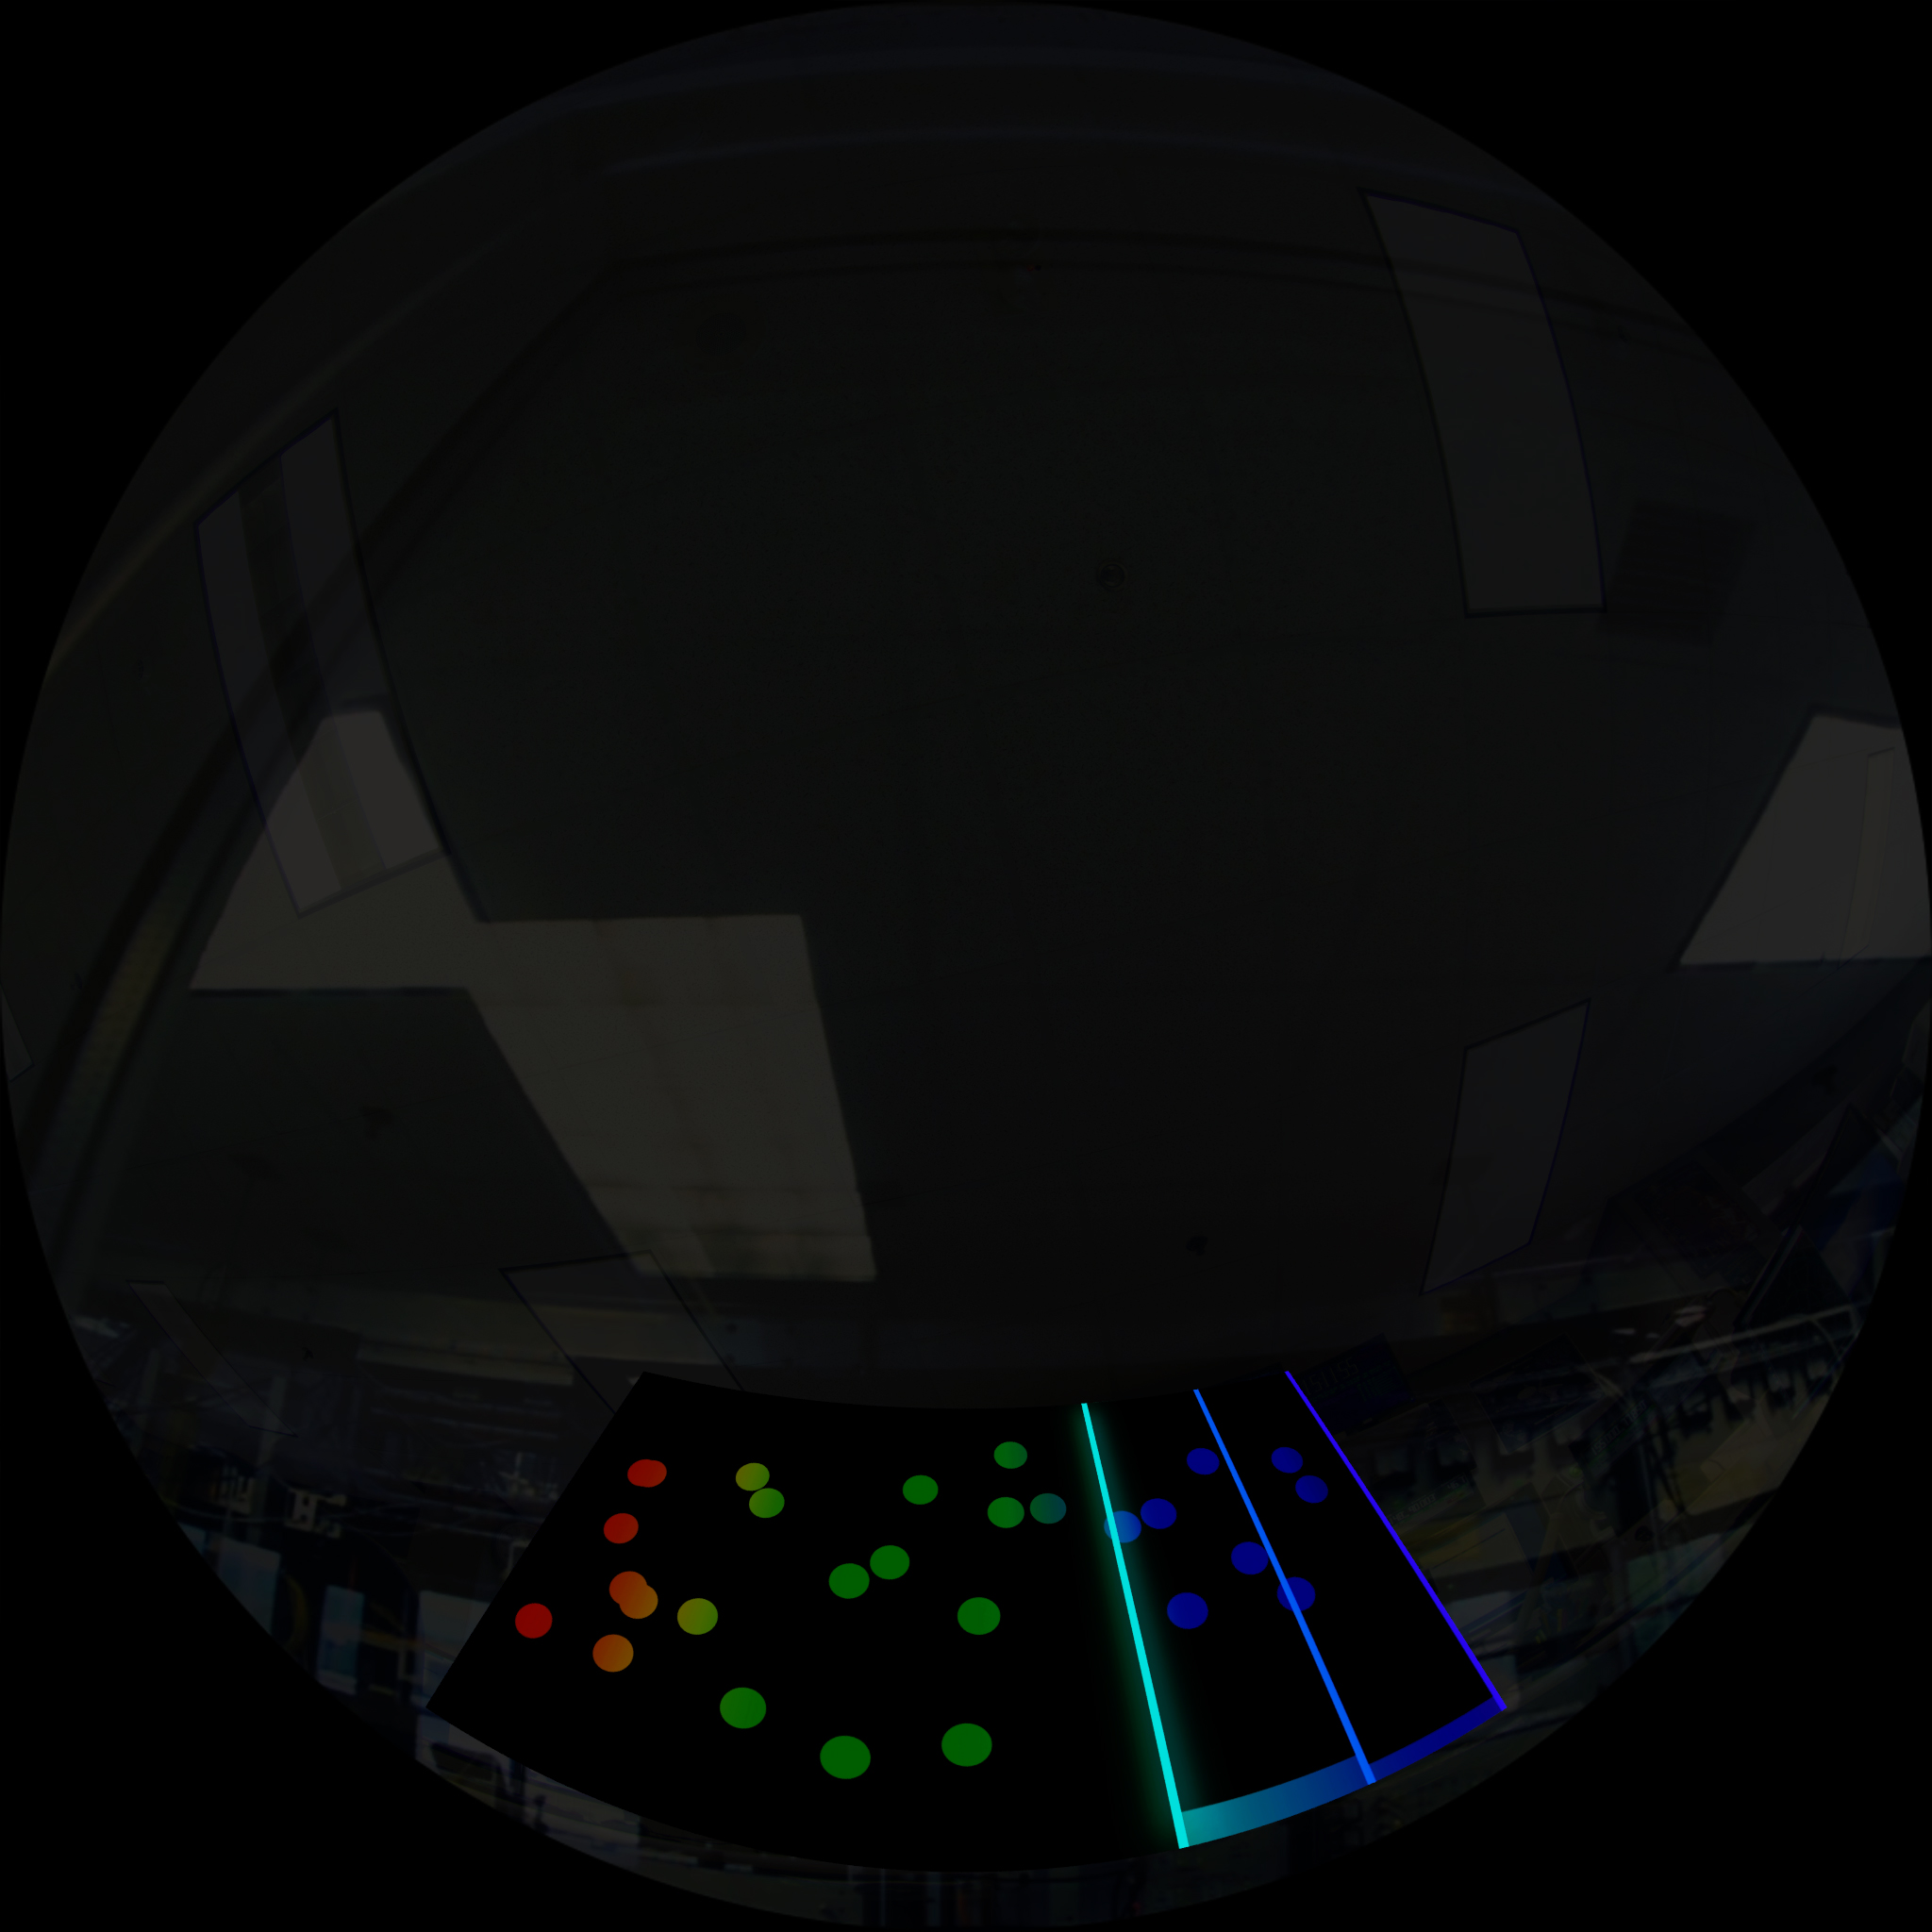
\includegraphics[width=0.3\textwidth]{Planetarium/figures/script_shots/shot20.jpg}} \vspace{0.1cm}\\ 

\hline

\textit{The telescope looks at a different part of the sky in each second. So we build an image of the sky, one point at a time. }& 

\raisebox{-\totalheight}{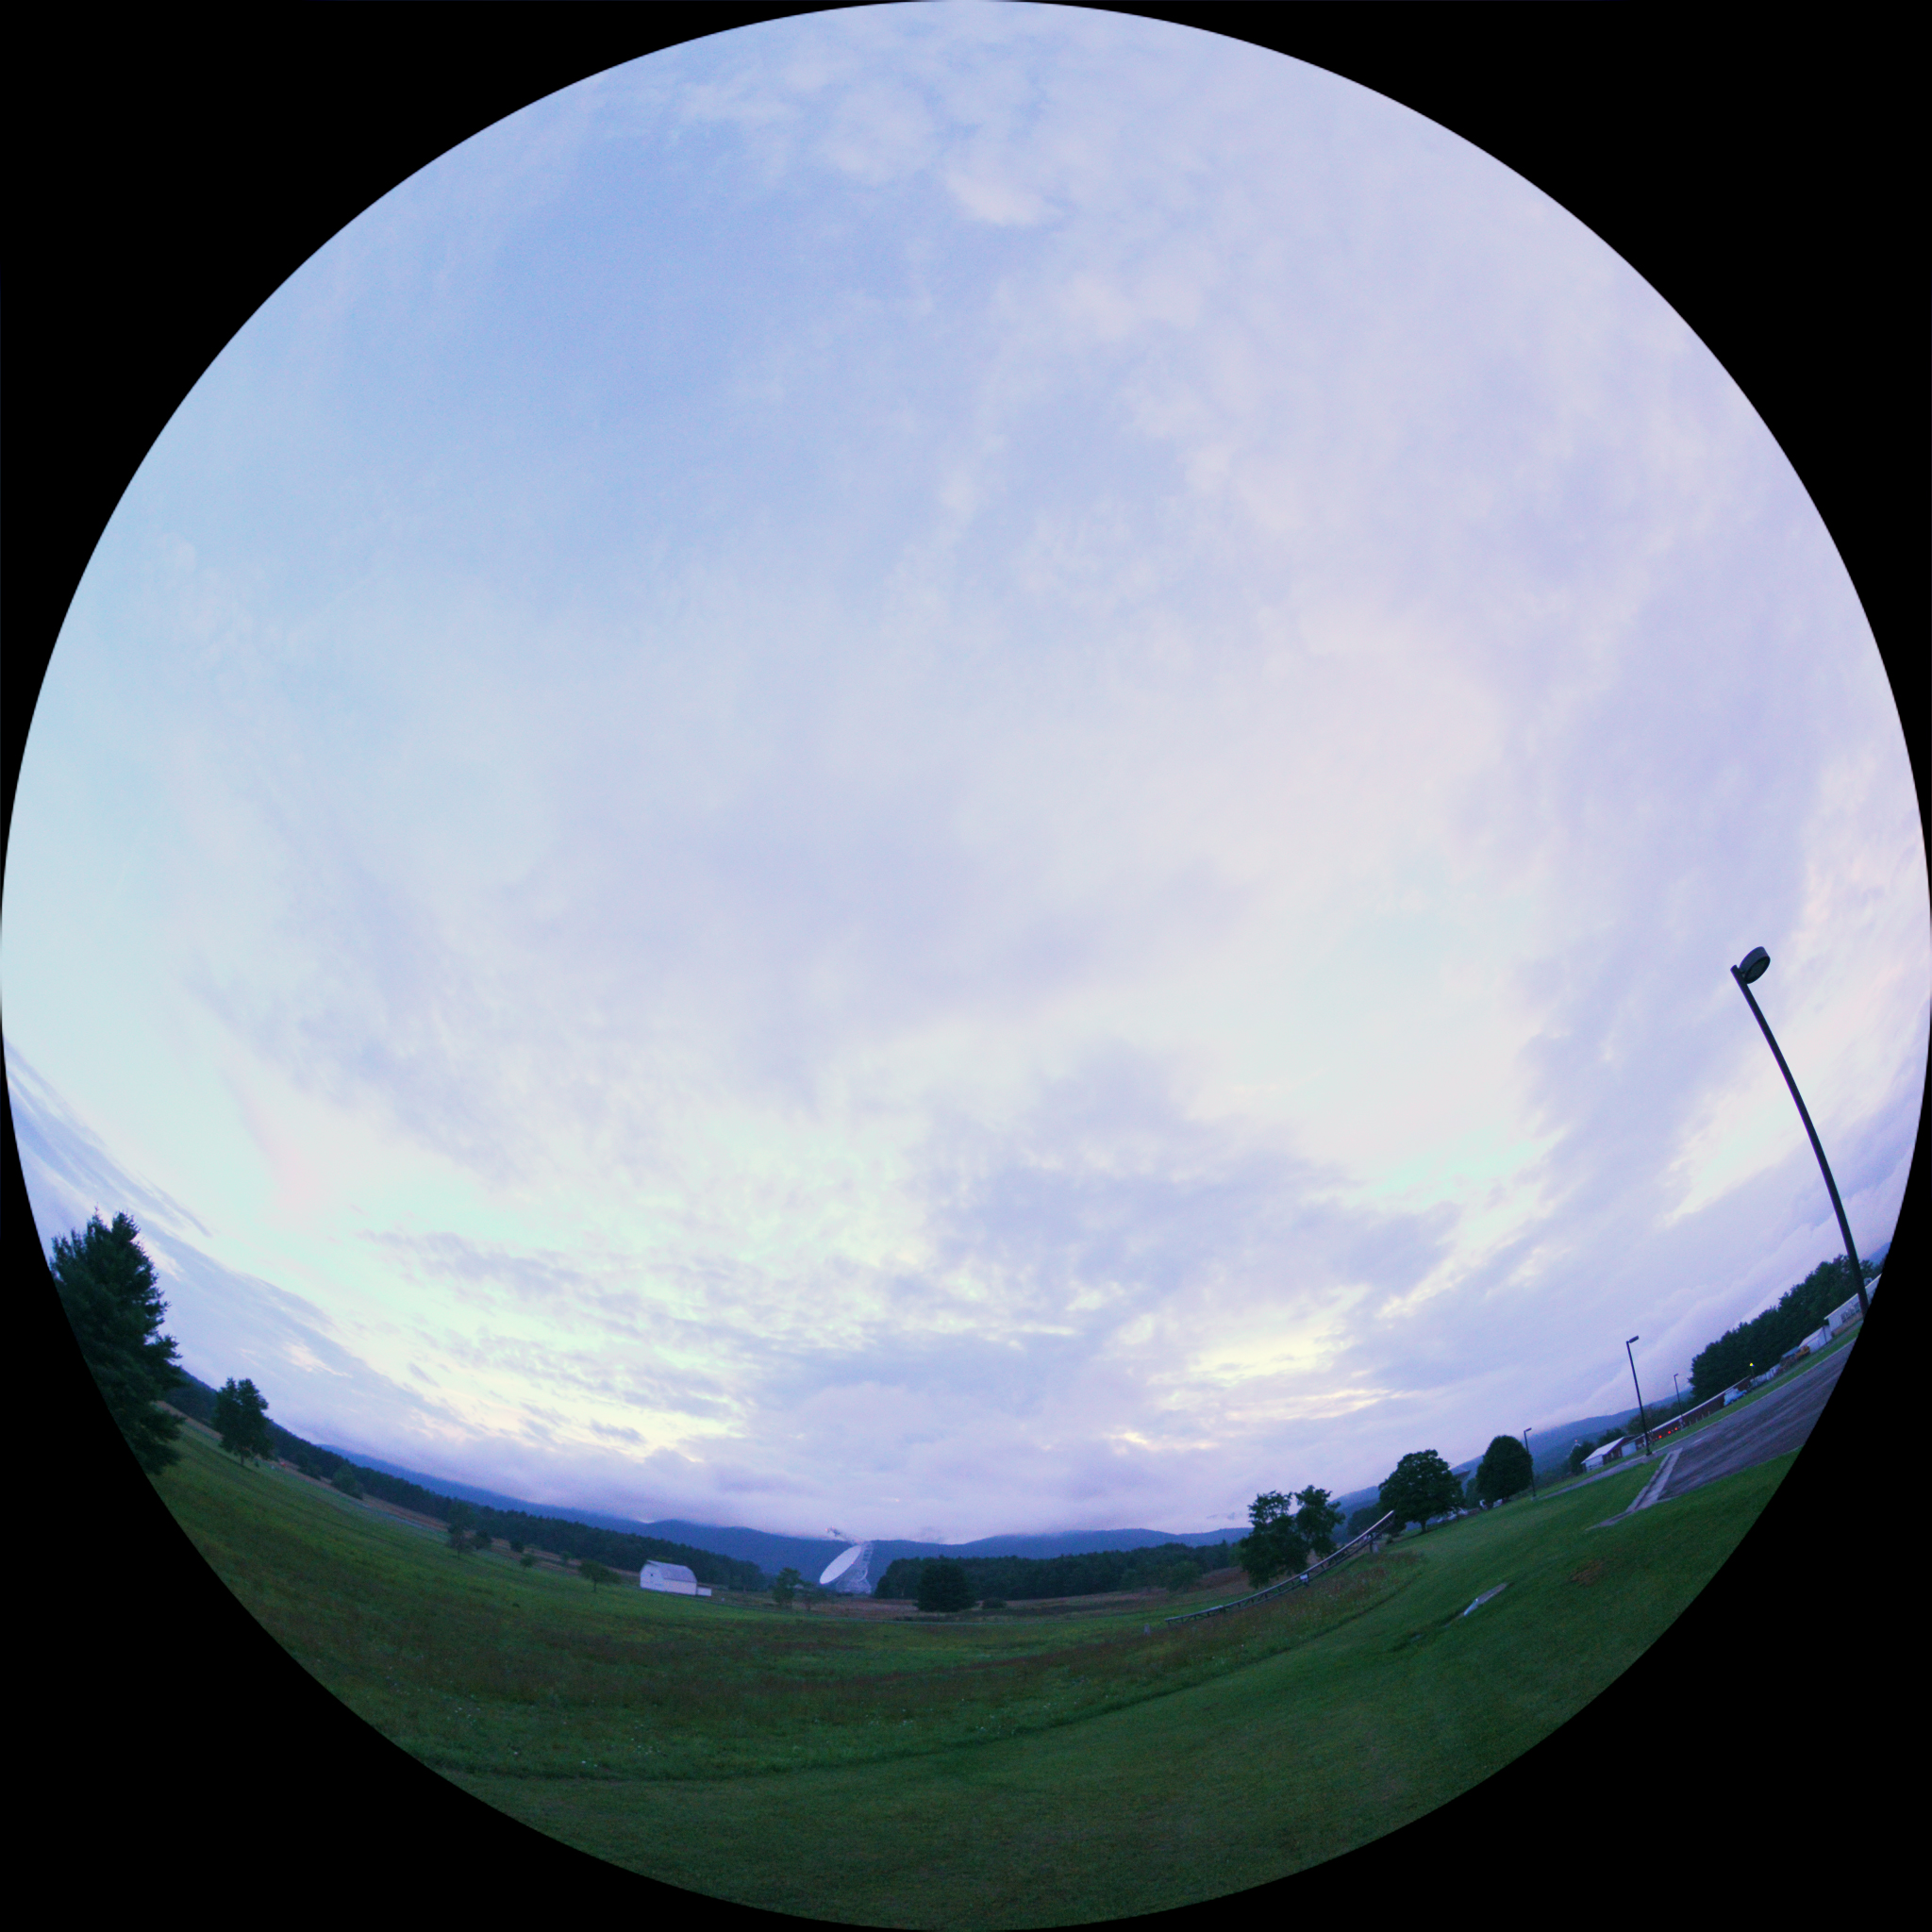
\includegraphics[width=0.3\textwidth]{Planetarium/figures/script_shots/shot21.jpg}} \vspace{0.1cm}\\

\hline

\textit{The brightest objects in the sky are nearby things, like the stars in the Milky Way Galaxy. If we want to see dimmer things, like the photons from Hydrogen clouds around distant galaxies; we have to remove the bright stuff.} & 

\raisebox{-\totalheight}{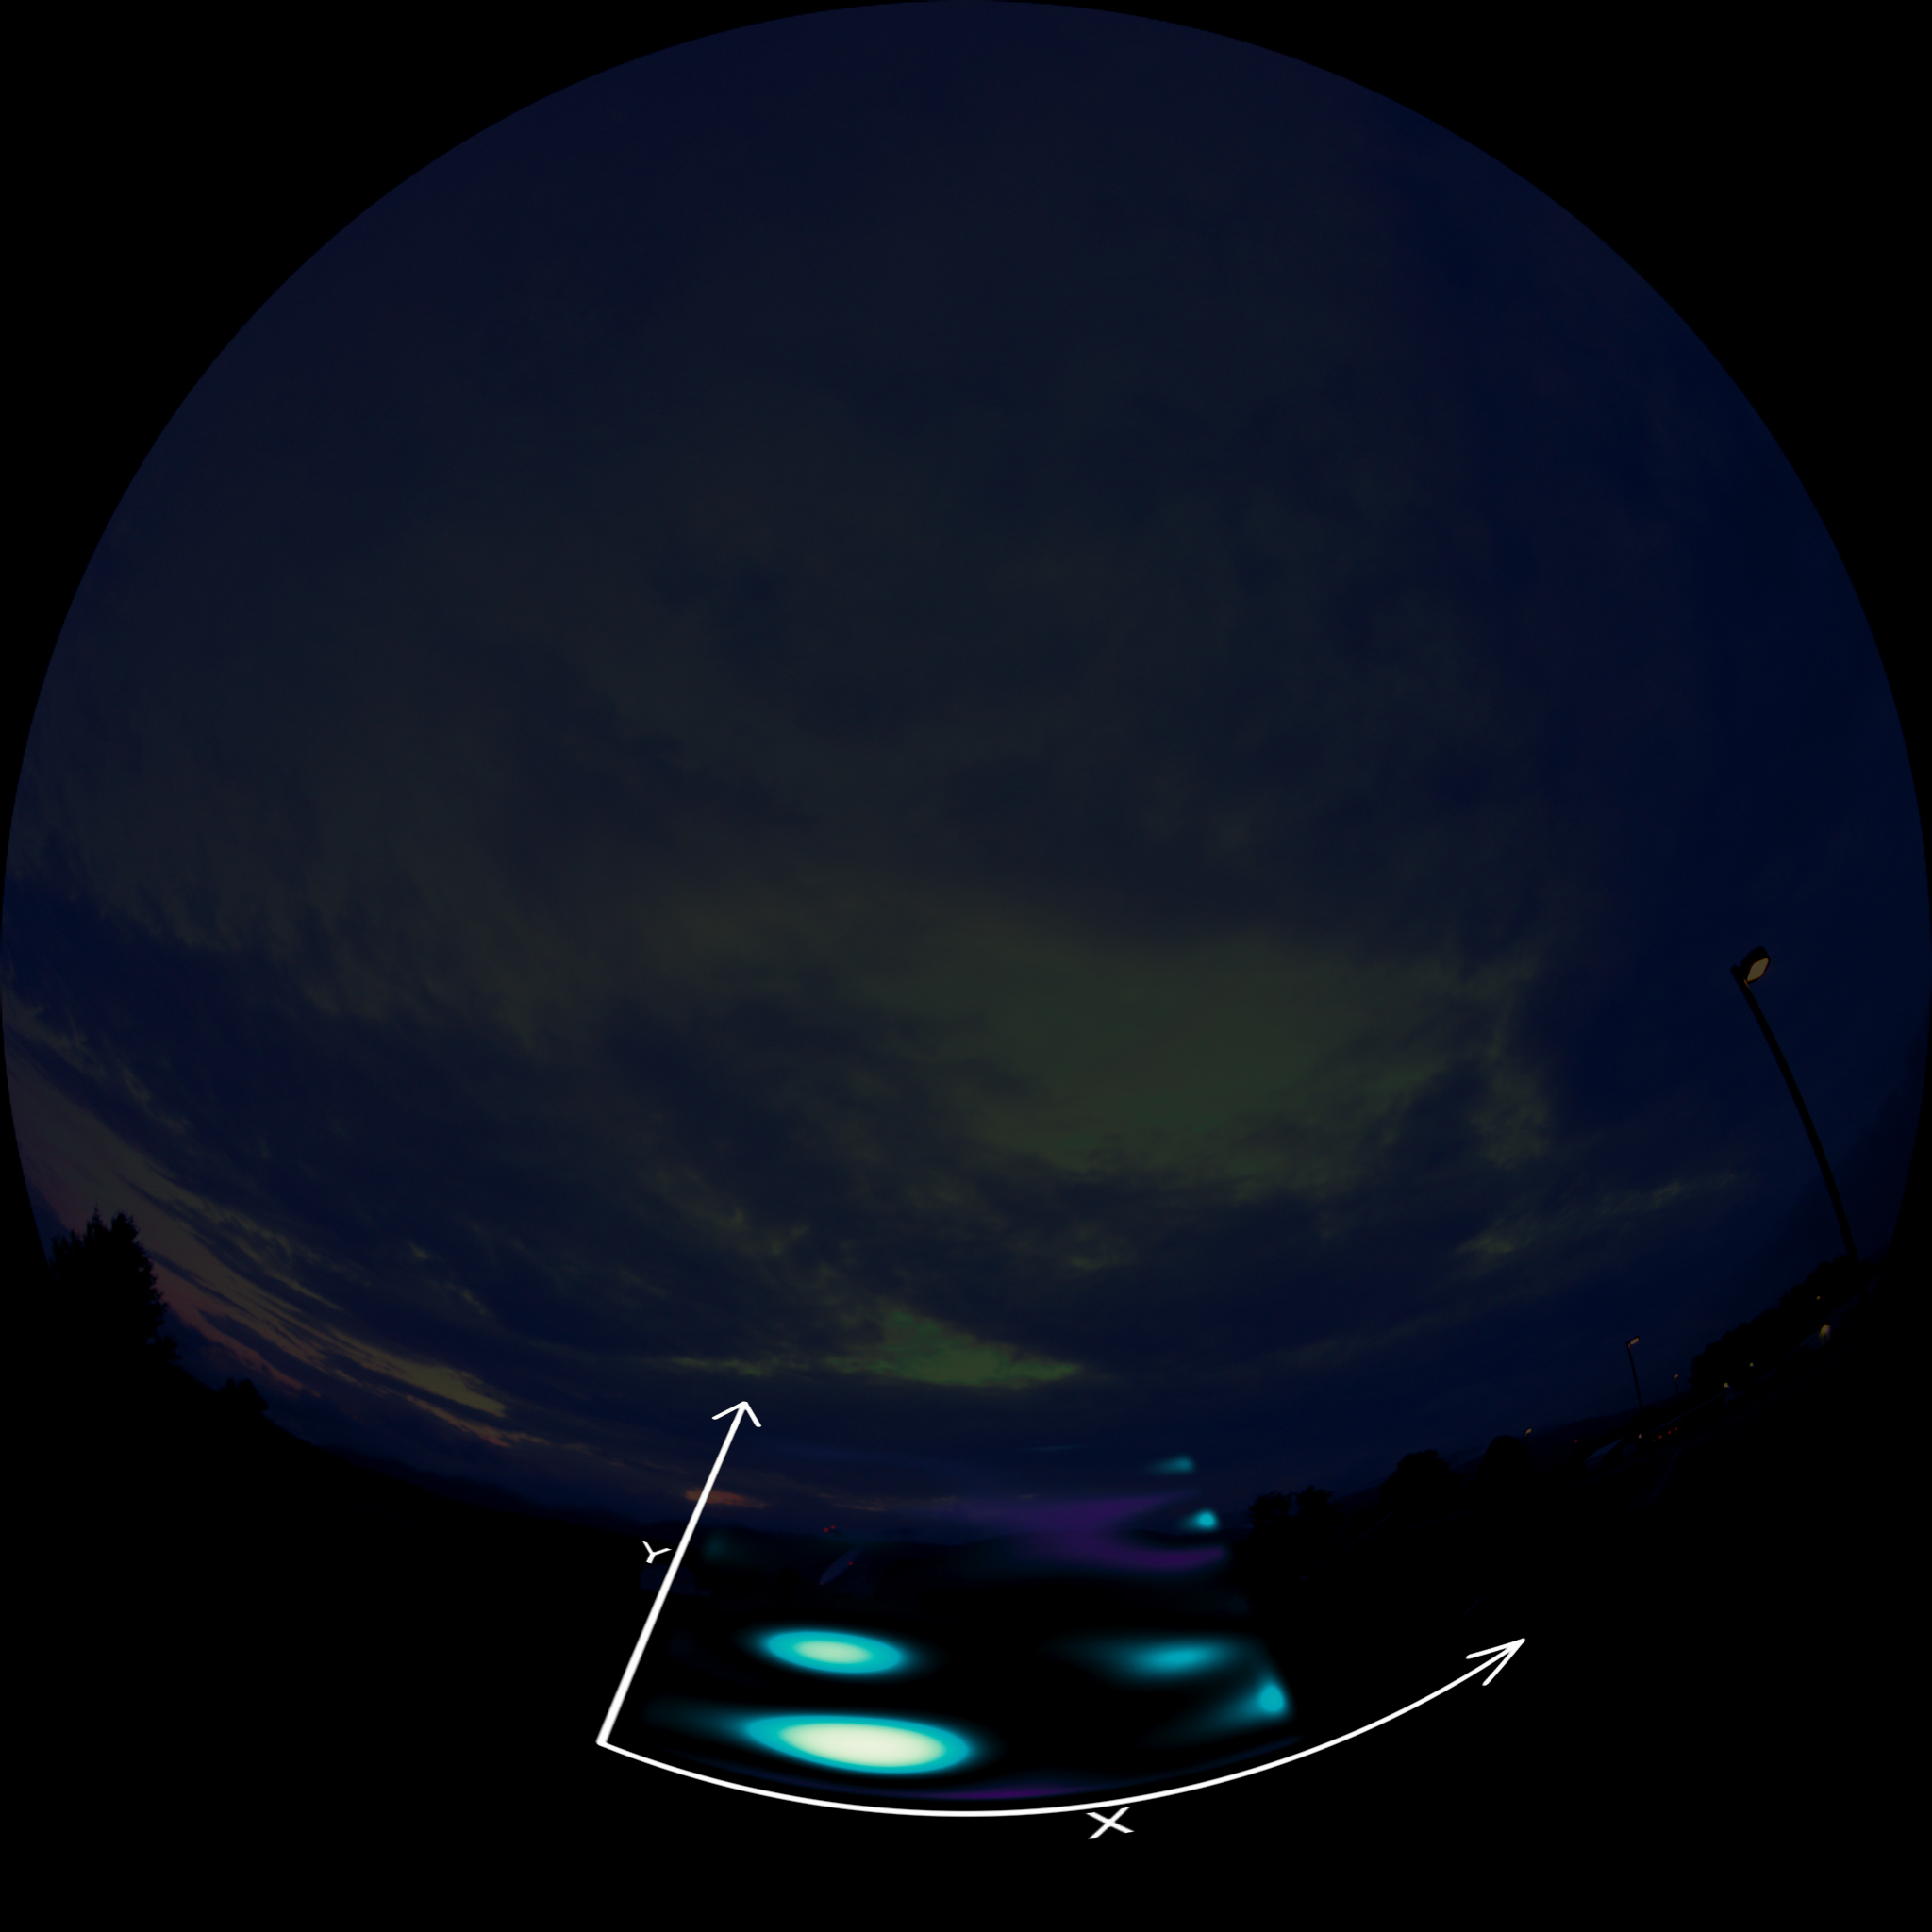
\includegraphics[width=0.3\textwidth]{Planetarium/figures/script_shots/shot22.jpg}} \vspace{0.1cm}\\

\hline

\textit{We can do this thanks to redshifting, which changes the wavelength of the photons from the Hydrogen clouds.  }& 

\raisebox{-\totalheight}{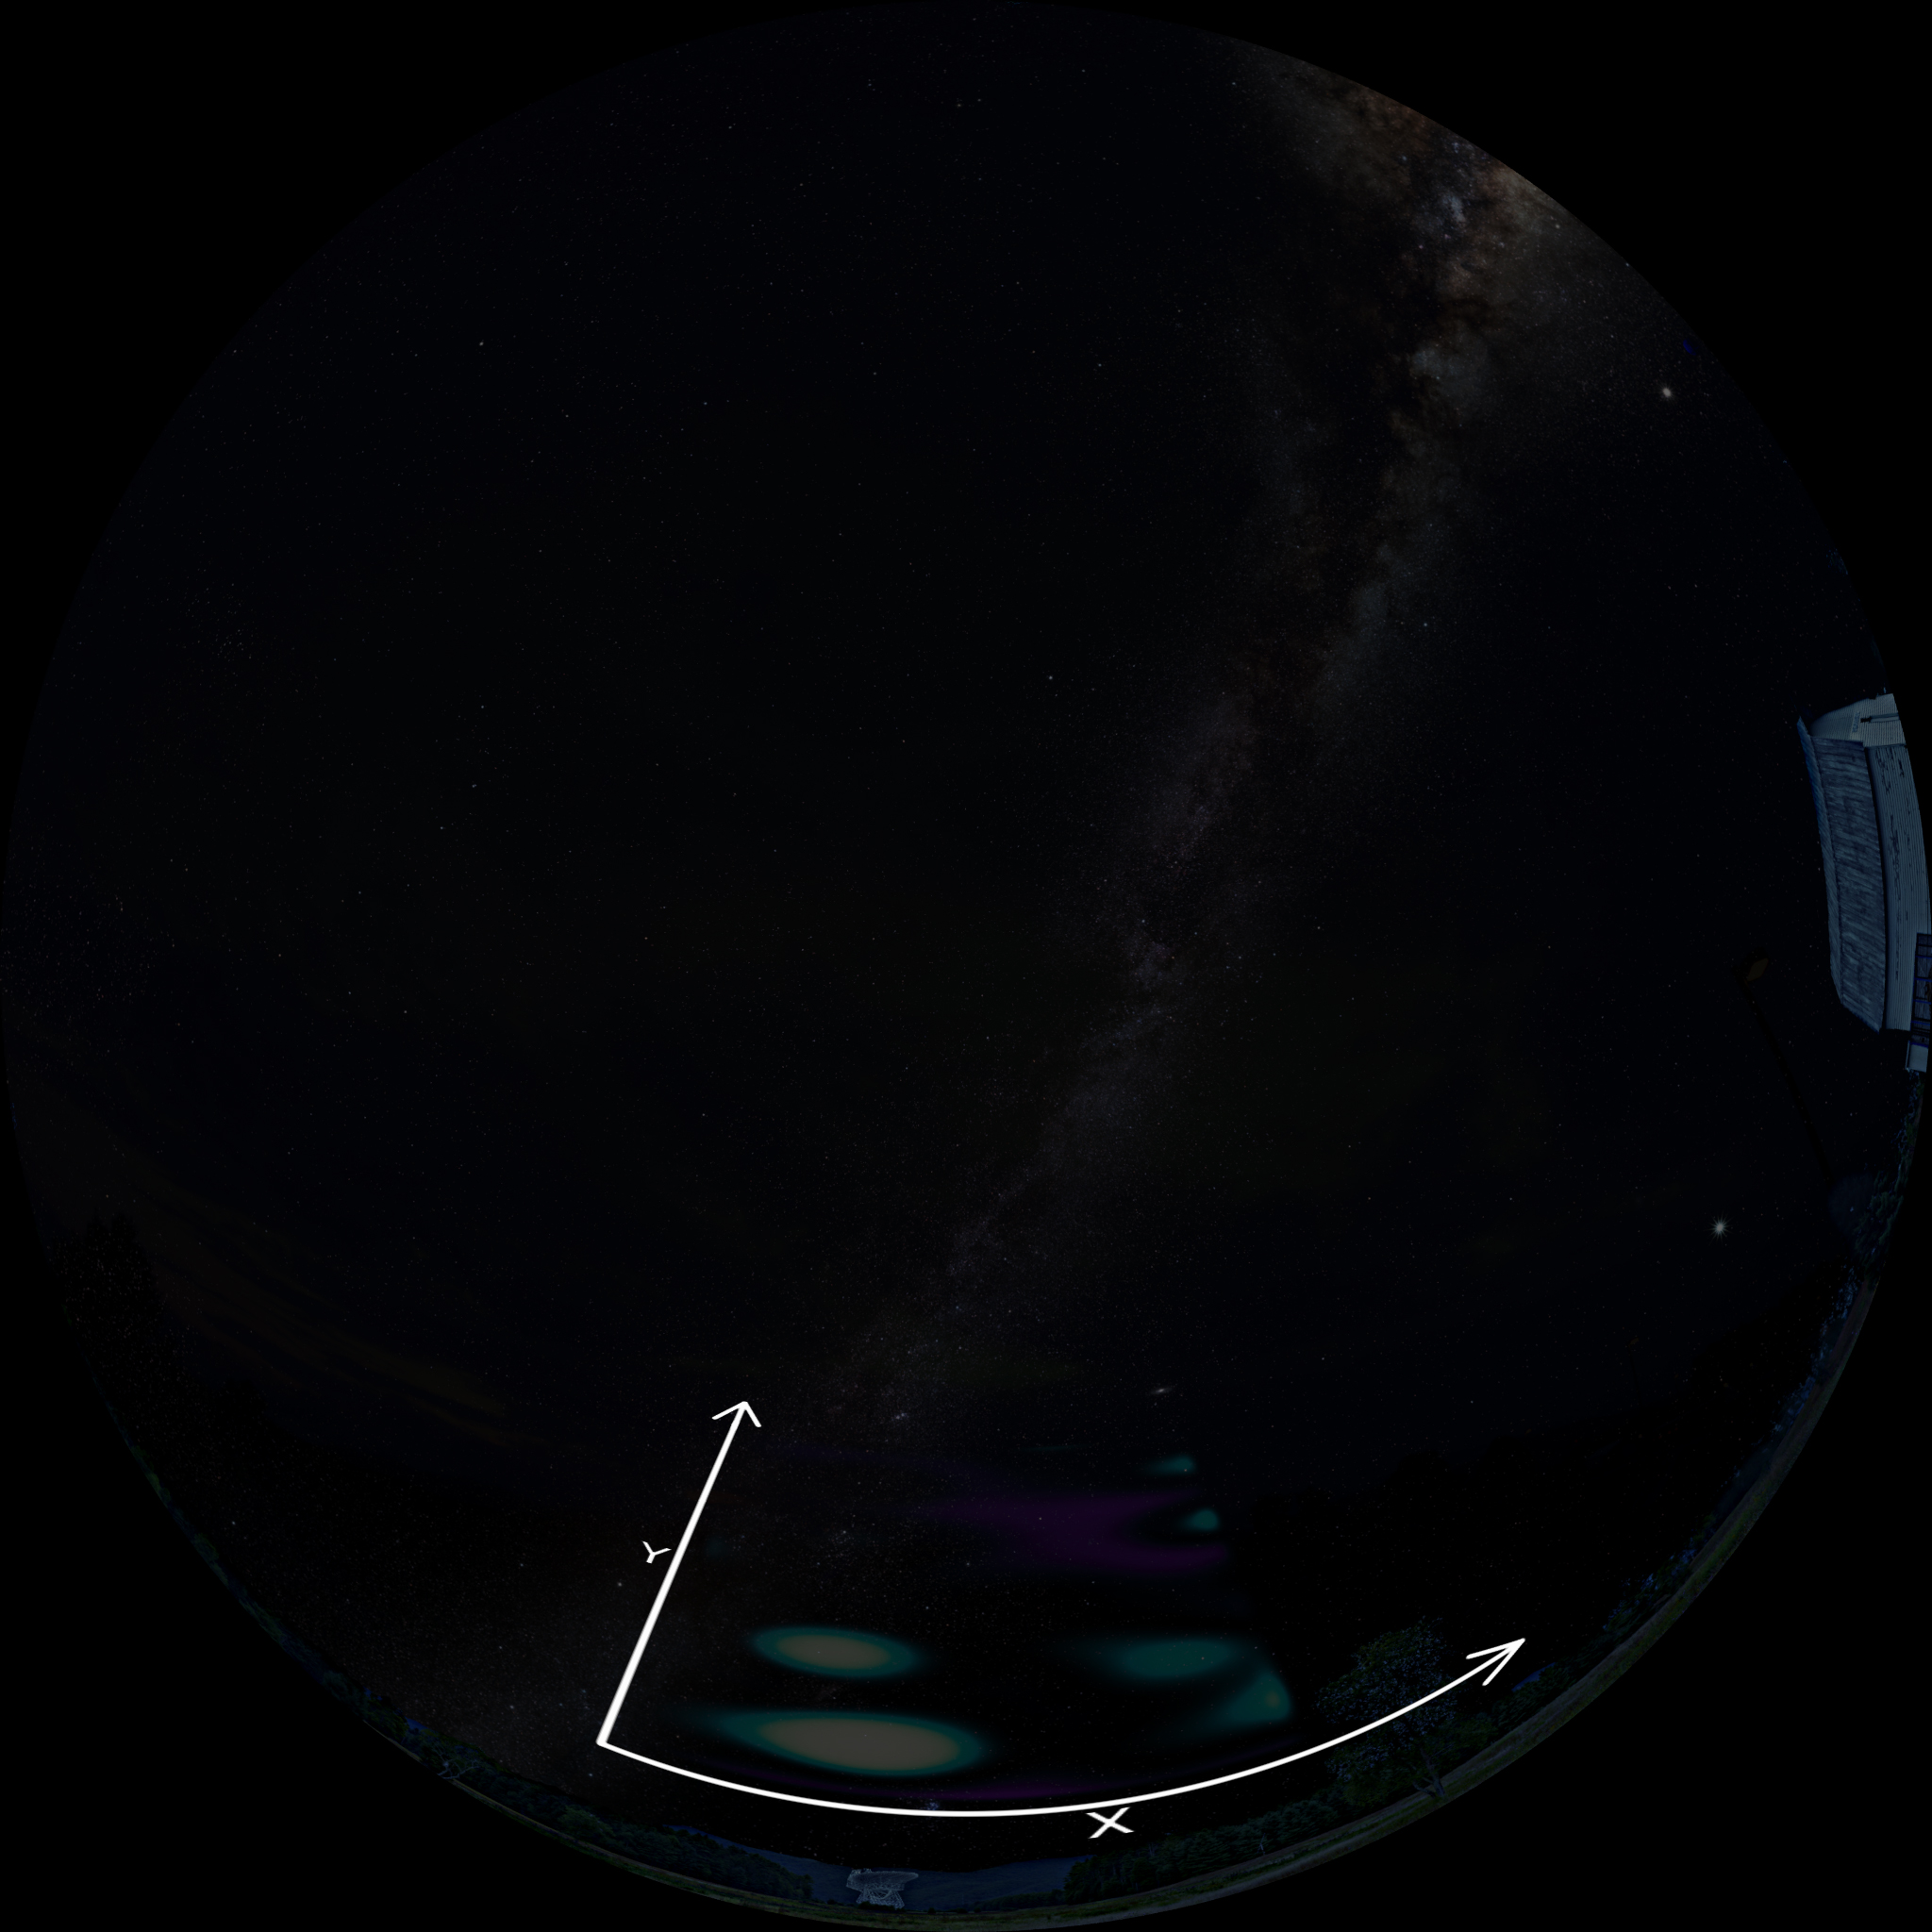
\includegraphics[width=0.3\textwidth]{Planetarium/figures/script_shots/shot23.jpg}} \vspace{0.1cm}\\

\hline

\textit{Unlike the bright nearby stars that produce light at all wavelengths; photons from the Hydrogen clouds have a specific wavelength. }& 

\raisebox{-\totalheight}{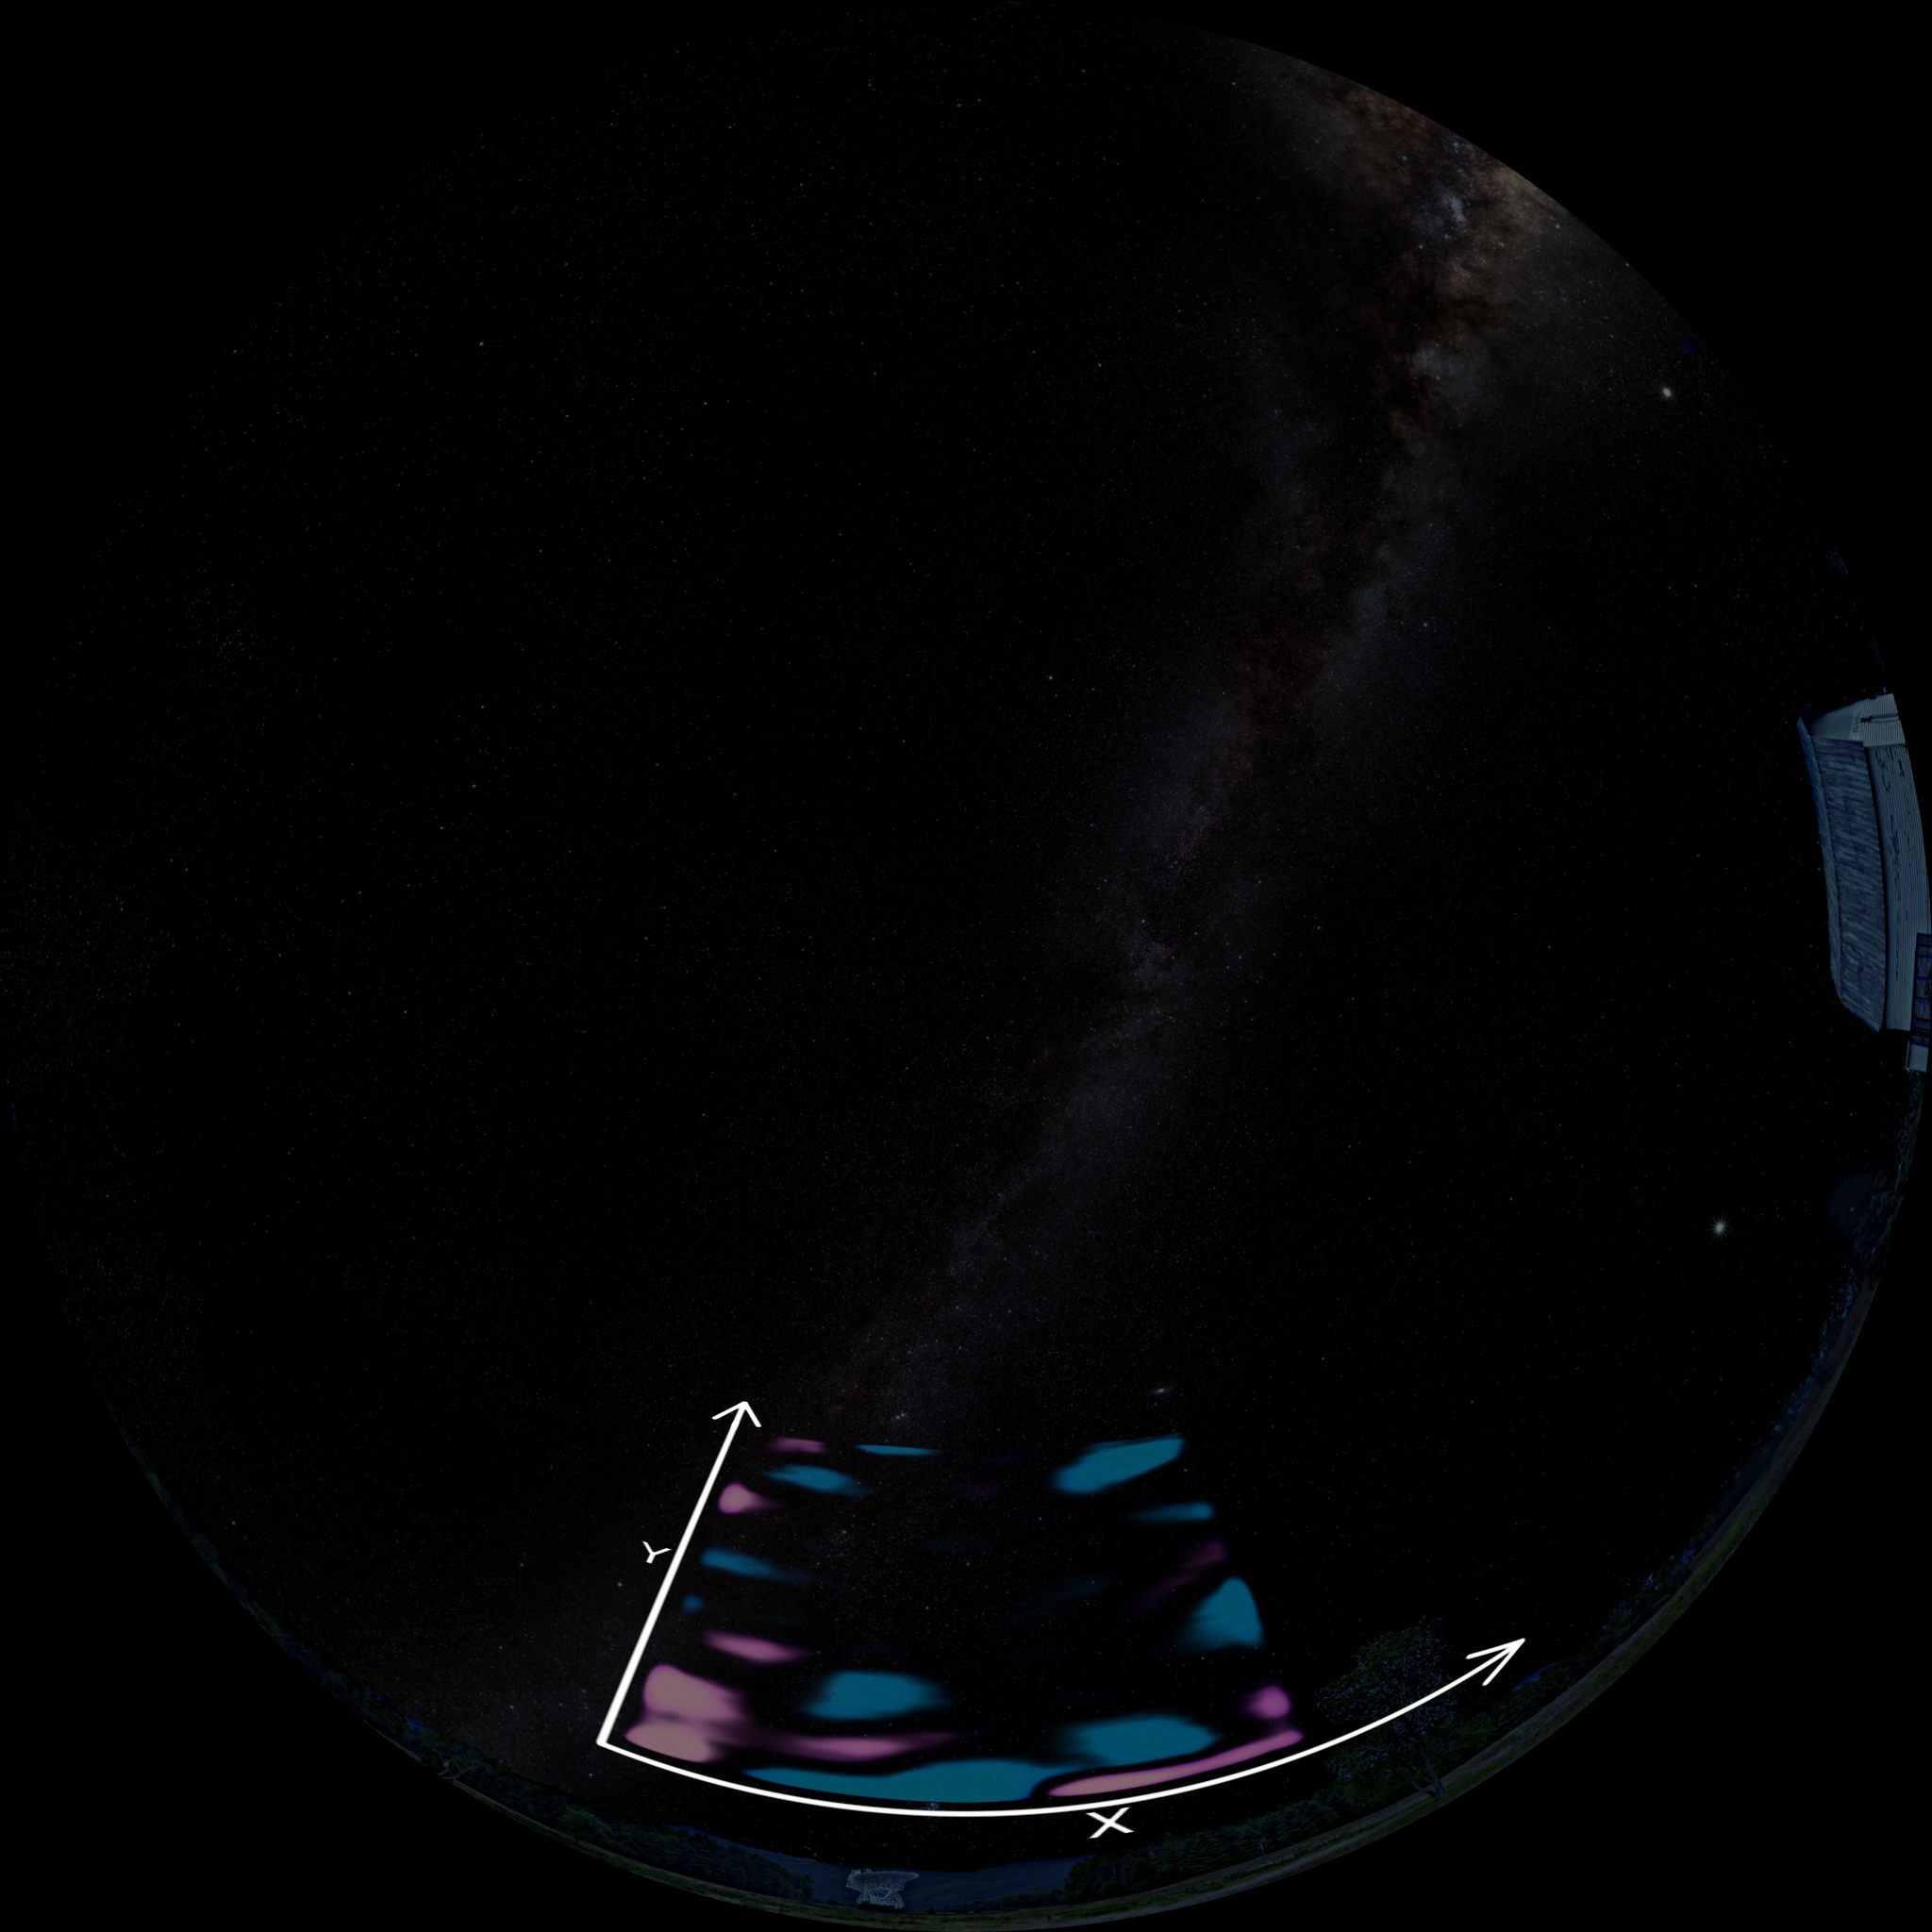
\includegraphics[width=0.3\textwidth]{Planetarium/figures/script_shots/shot24.jpg}} \vspace{0.1cm}\\

\hline

\textit{More distant clouds have their photons wavelengths redshifted to longer wavelengths than closer clouds. In this way, we can separate the light from the Hydrogen sky from the light from nearby bright sources. }& 

\raisebox{-\totalheight}{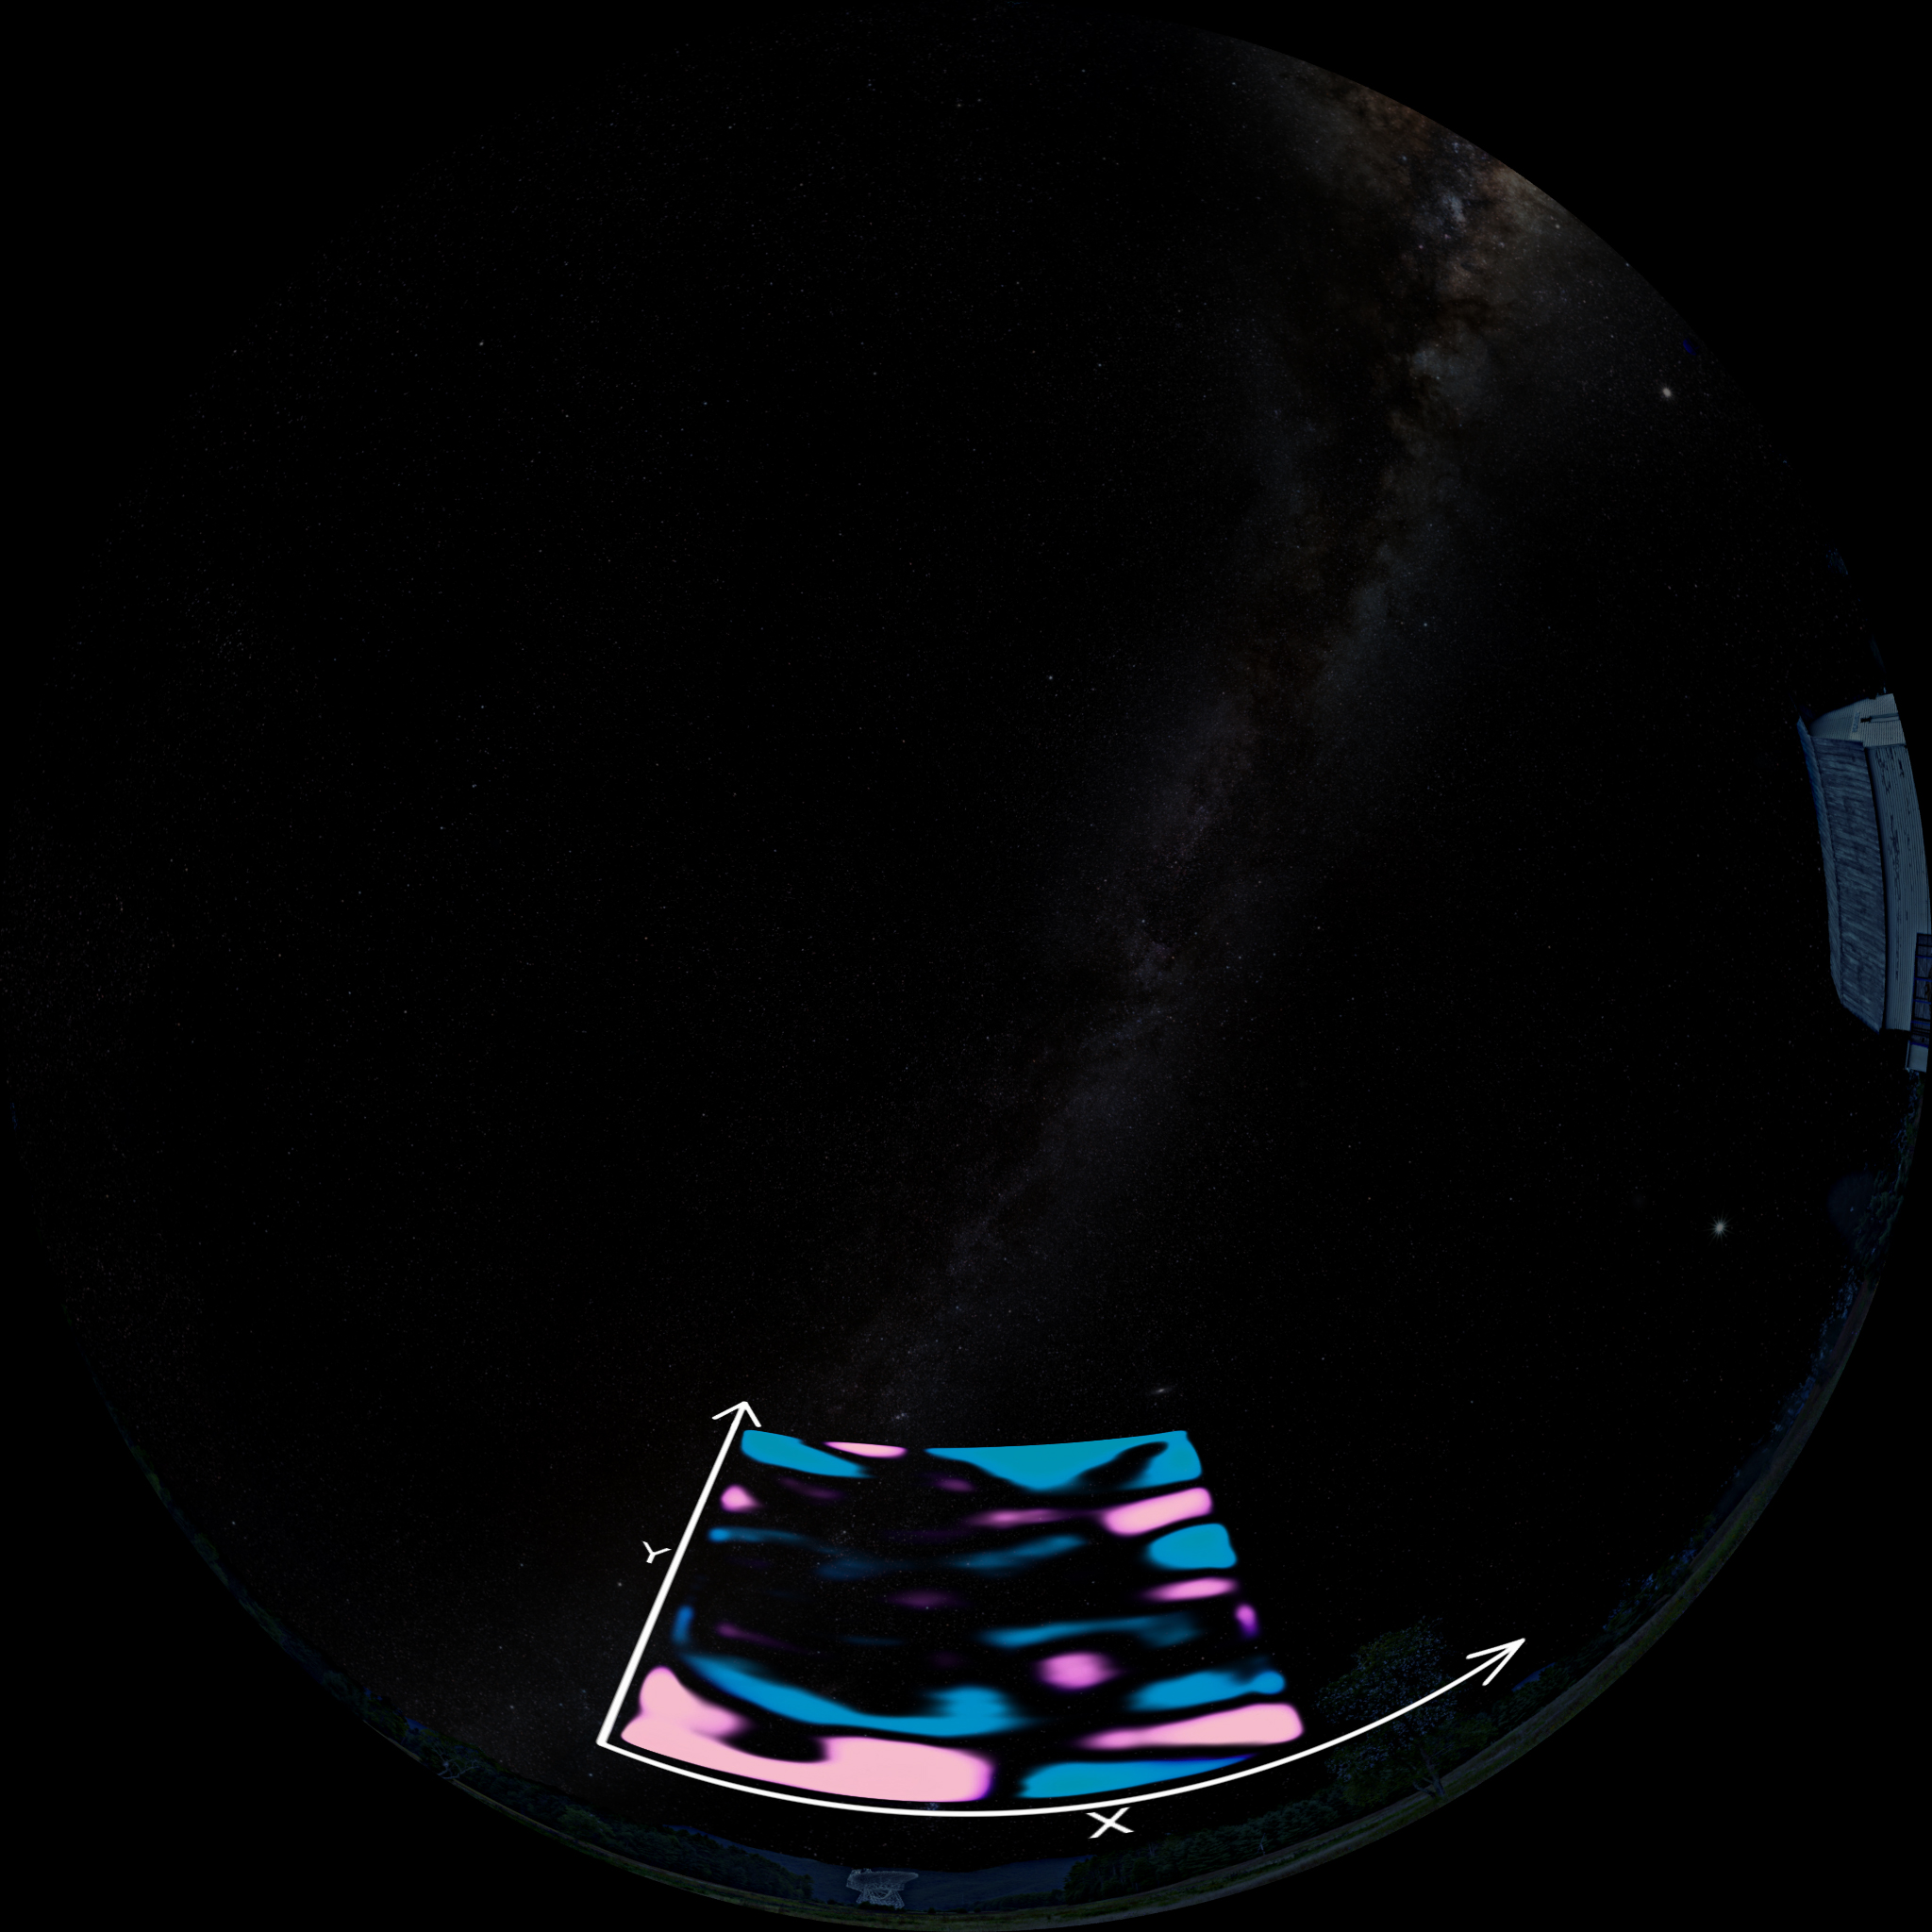
\includegraphics[width=0.3\textwidth]{Planetarium/figures/script_shots/shot25.jpg}} \vspace{0.1cm}\\

\hline

\textit{This allows us to build a three-dimensional map of the Hydrogen sky. In this map the longer, and more redshifted wavelengths show us the Hydrogen sky around younger and more distant galaxies. }& 

\raisebox{-\totalheight}{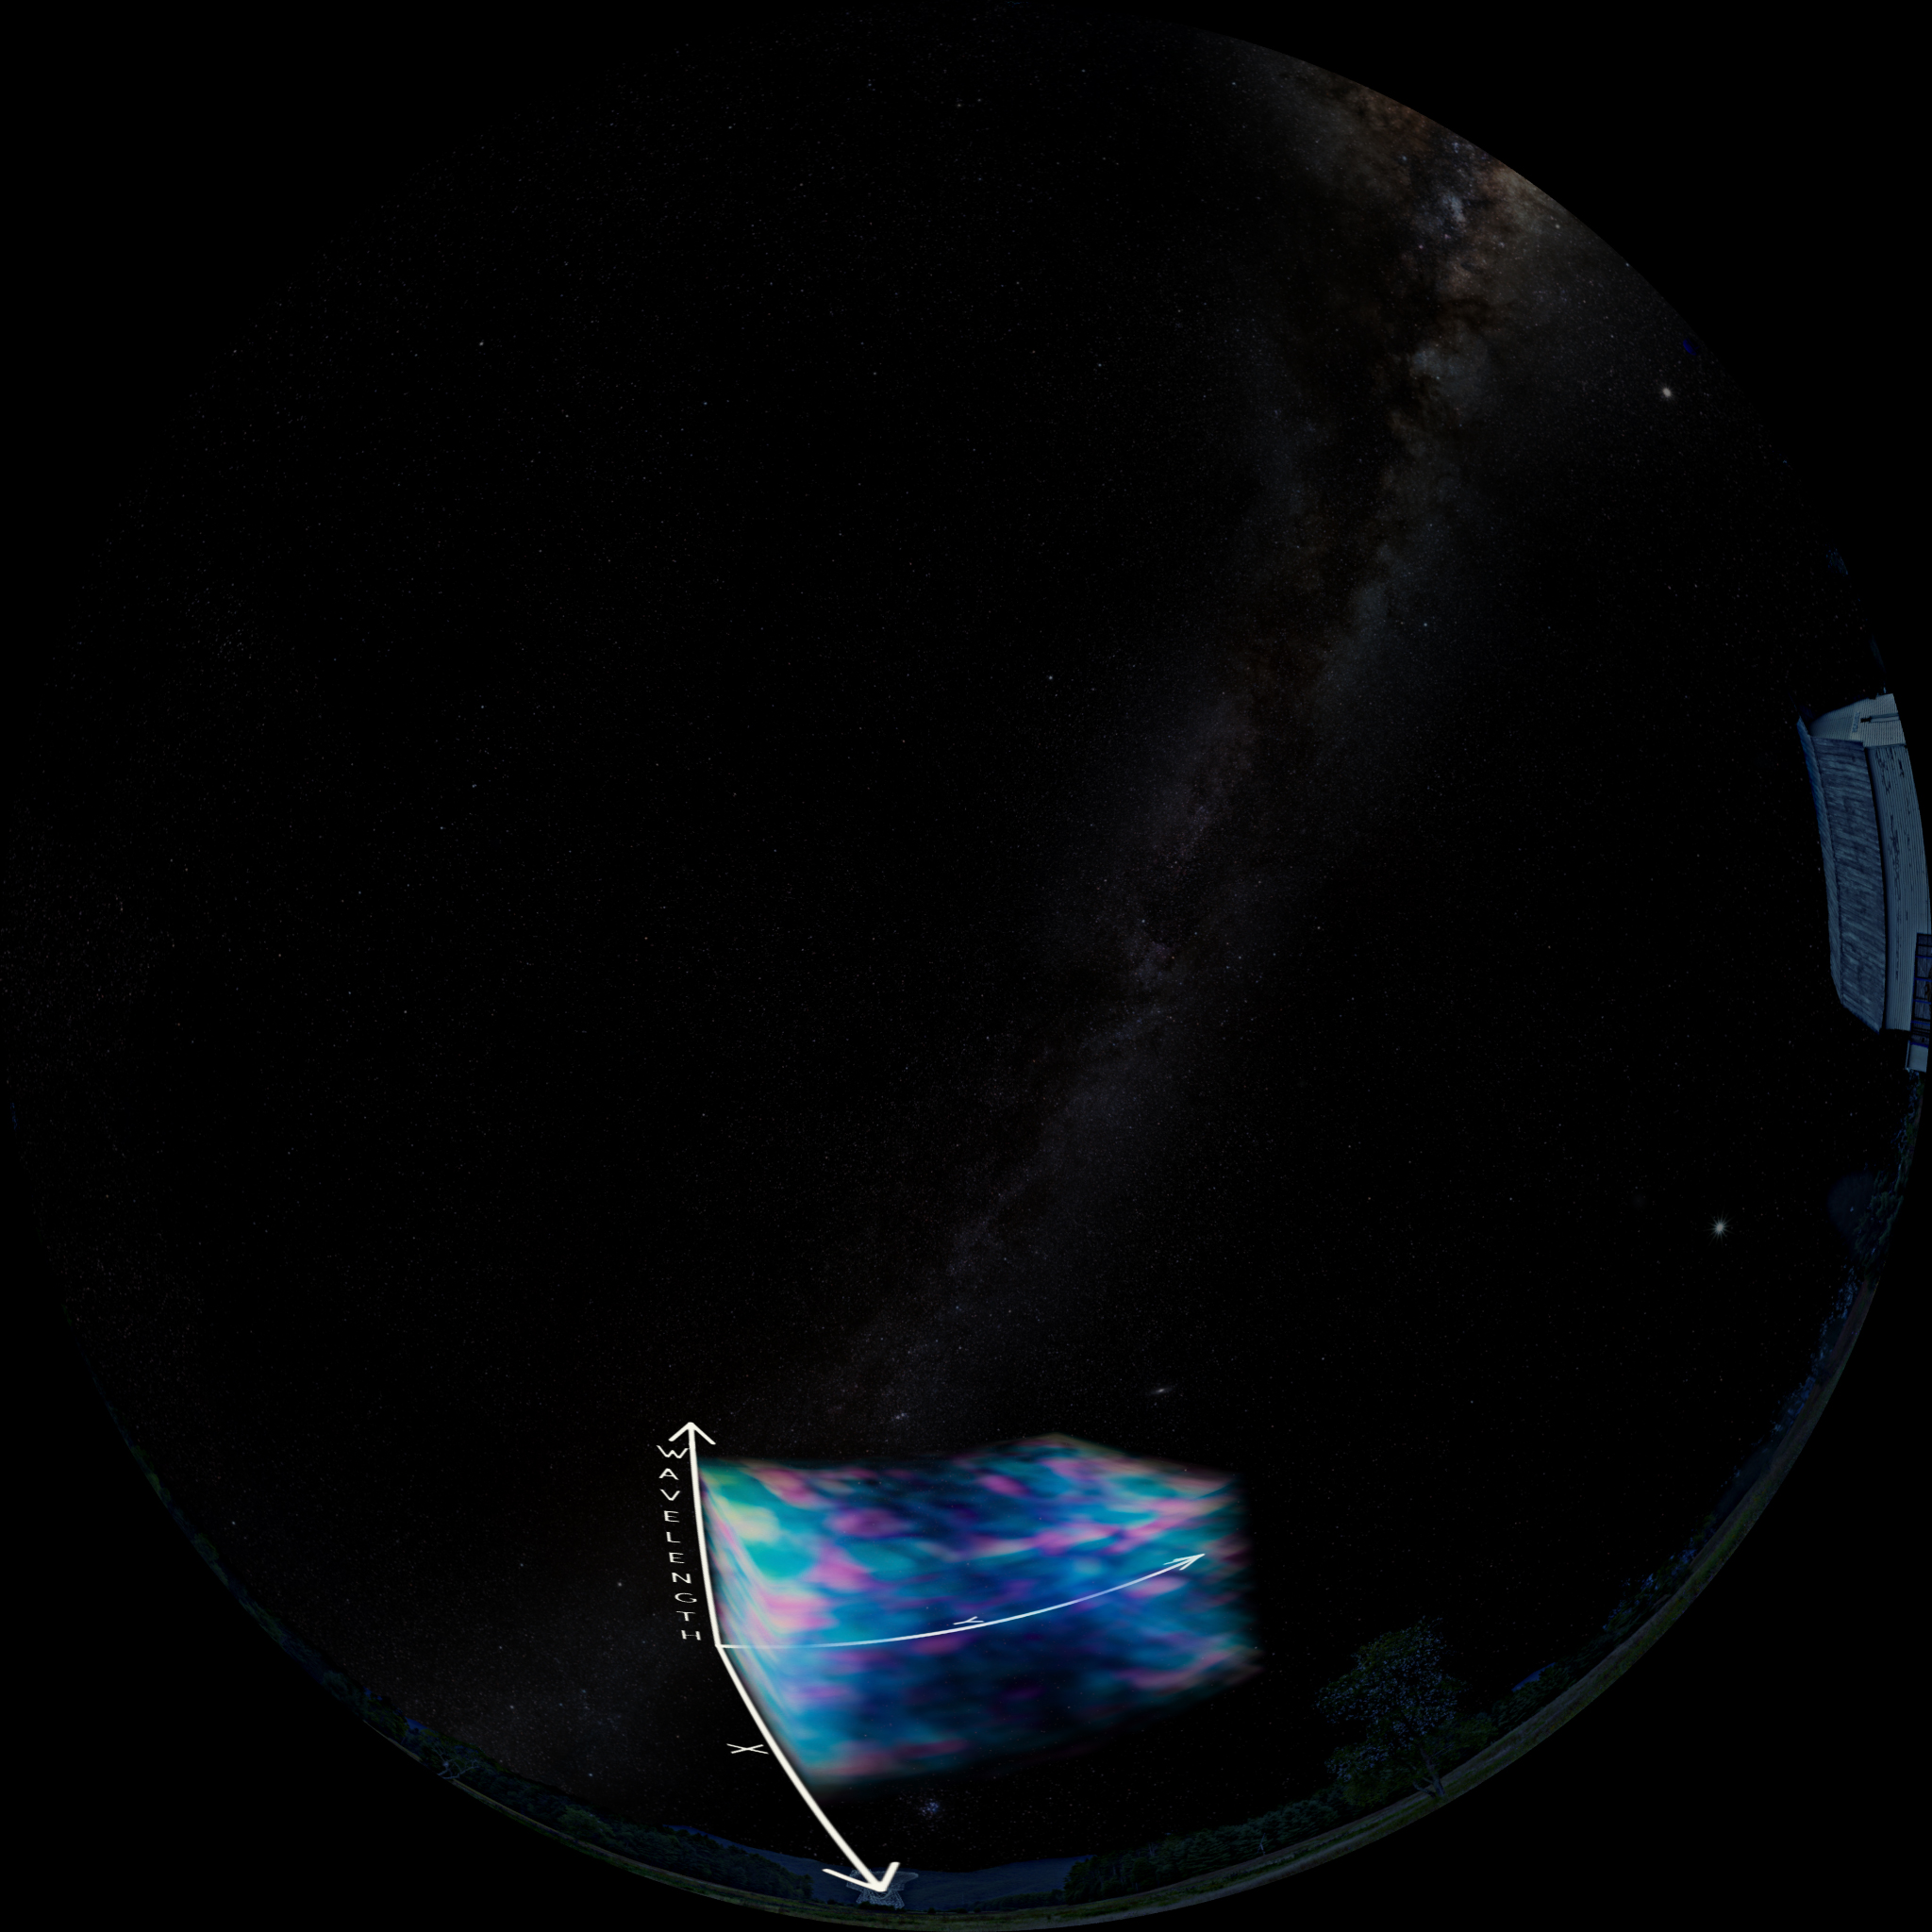
\includegraphics[width=0.3\textwidth]{Planetarium/figures/script_shots/shot26.jpg}} \vspace{0.1cm}\\

\hline

\textit{We spent over one hundred hours with the Green Bank Telescope collecting the light for this map. But the map only covers a very small fraction of the overall sky. To make maps of the whole sky we need to find faster ways to measure this light. } & 

\raisebox{-\totalheight}{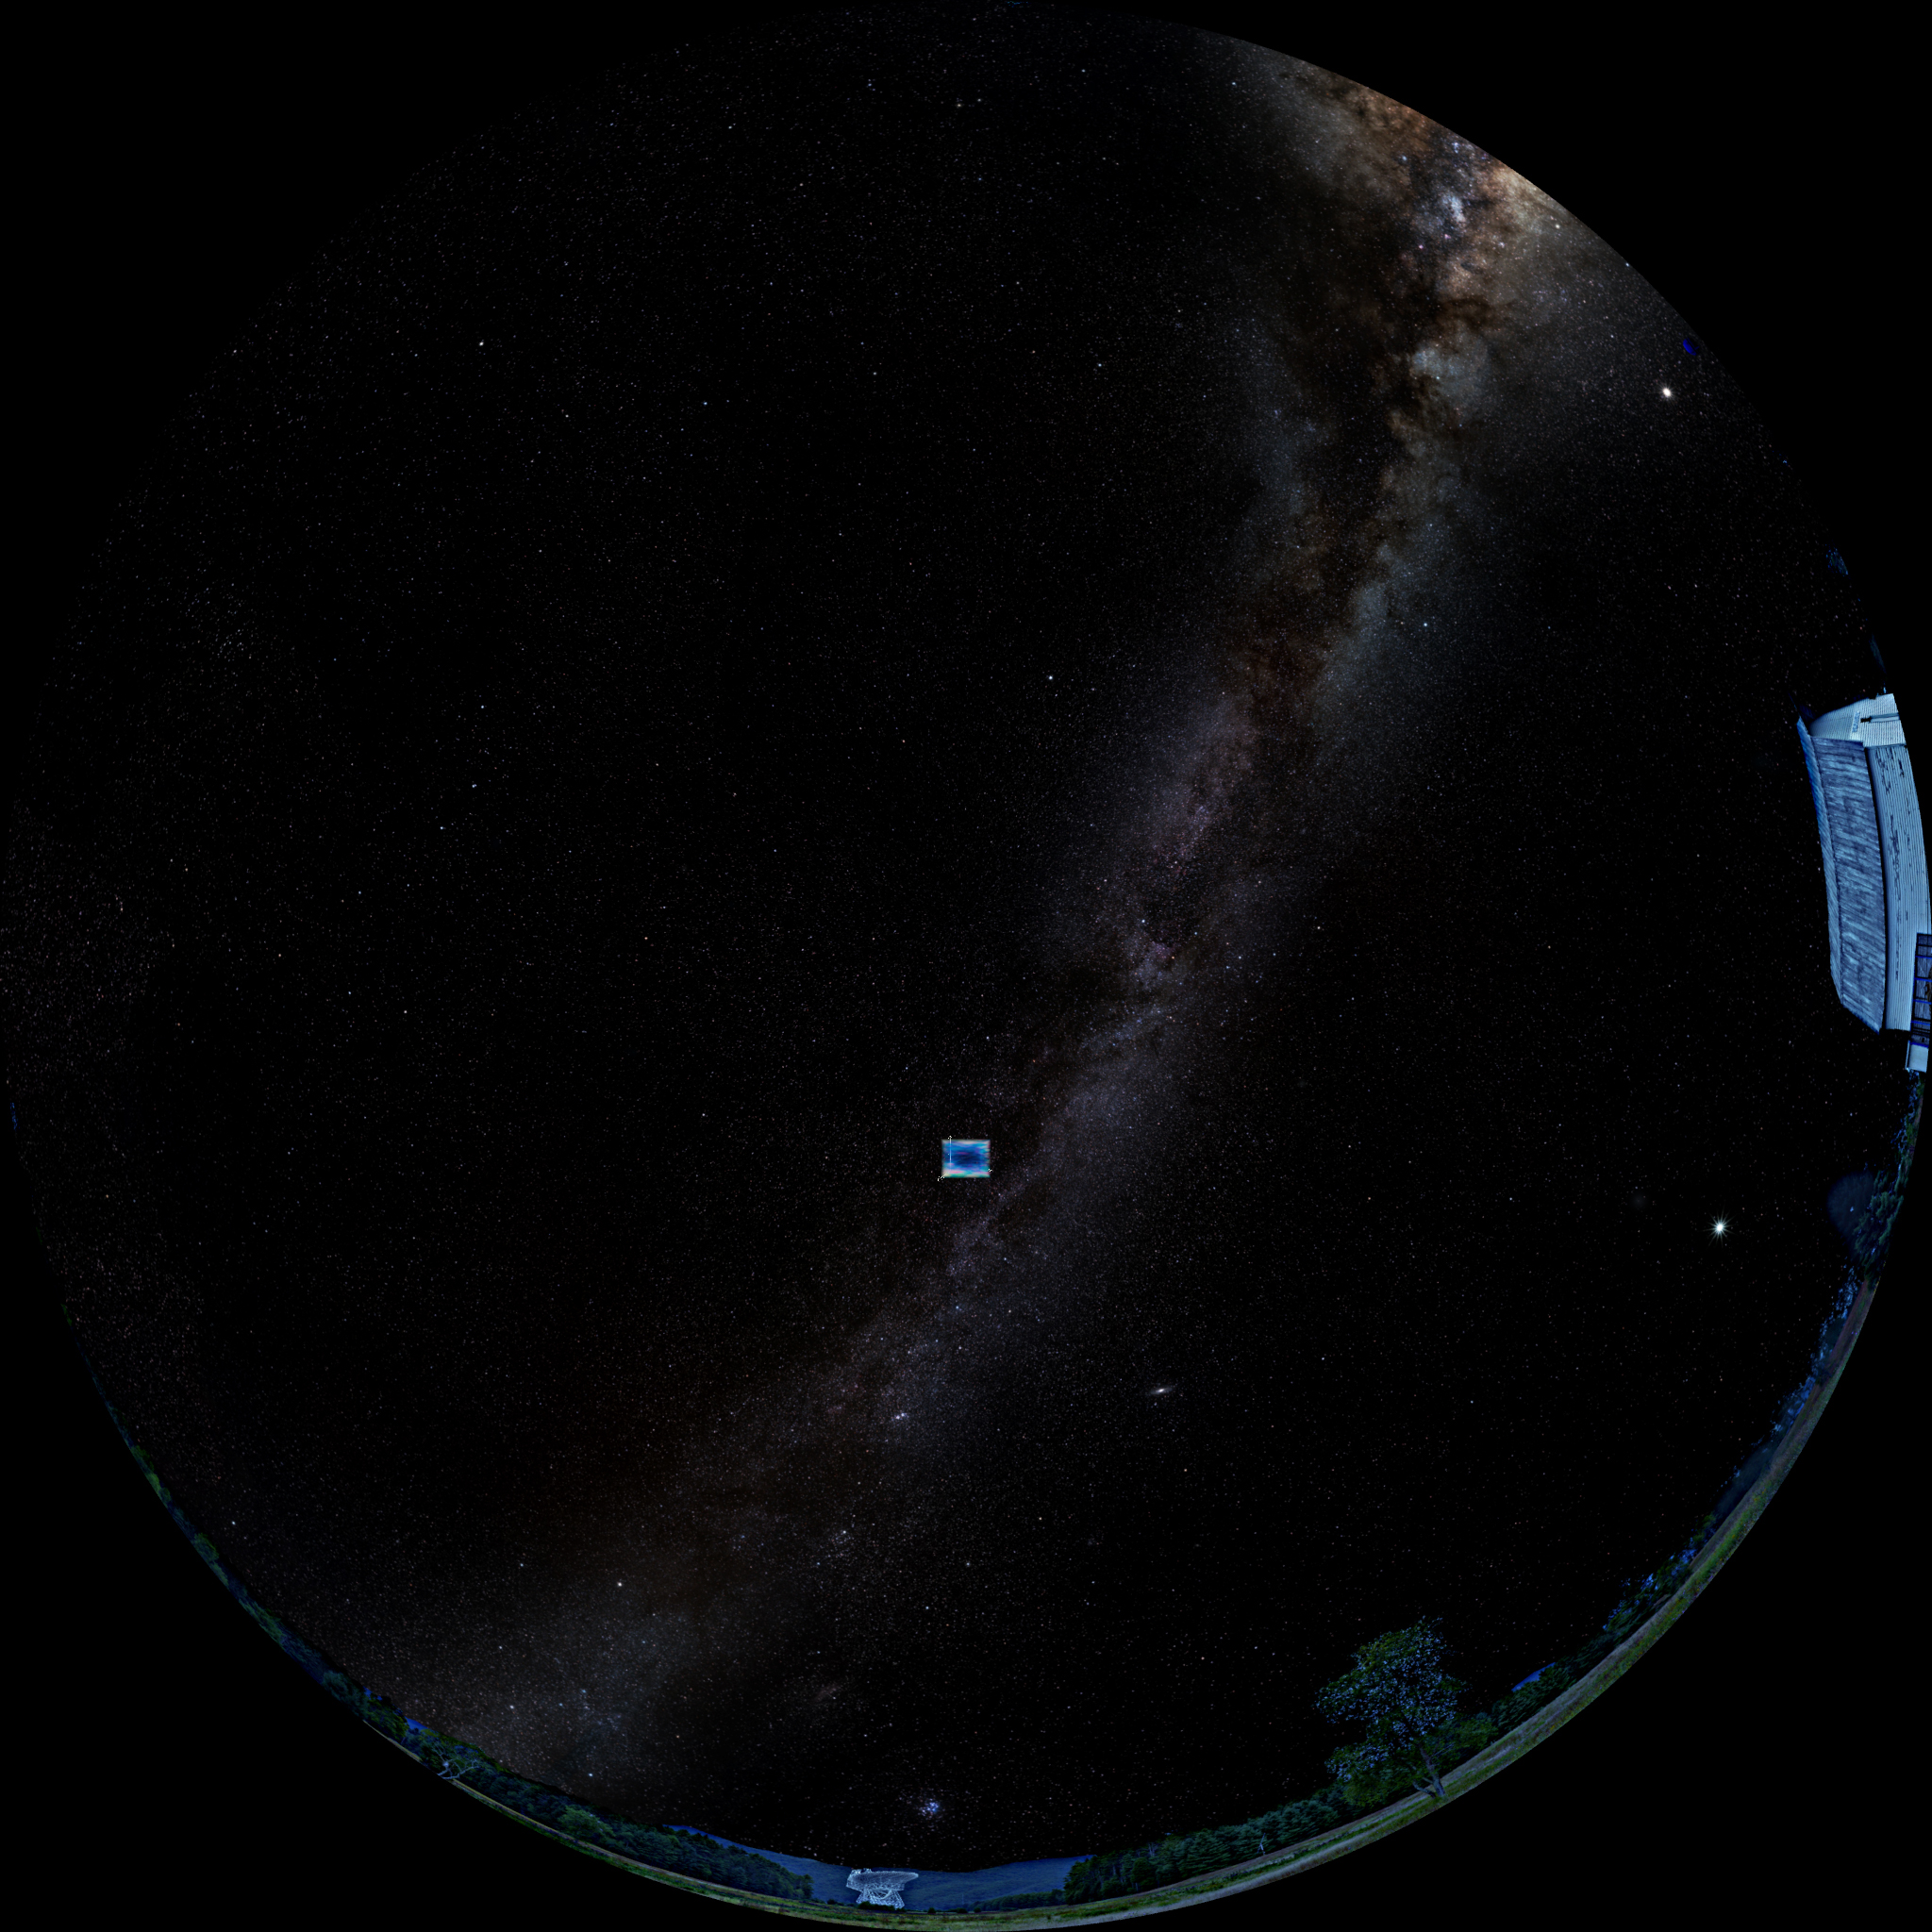
\includegraphics[width=0.3\textwidth]{Planetarium/figures/script_shots/shot27.jpg}} \vspace{0.1cm}\\

\hline

\textit{One way to do this is to build new radio telescopes which can look at multiple parts of the sky at the same time. The Canadian Hydrogen Intensity Mapping Experiment, or CHIME for short, is one such new telescope. }& 

\raisebox{-\totalheight}{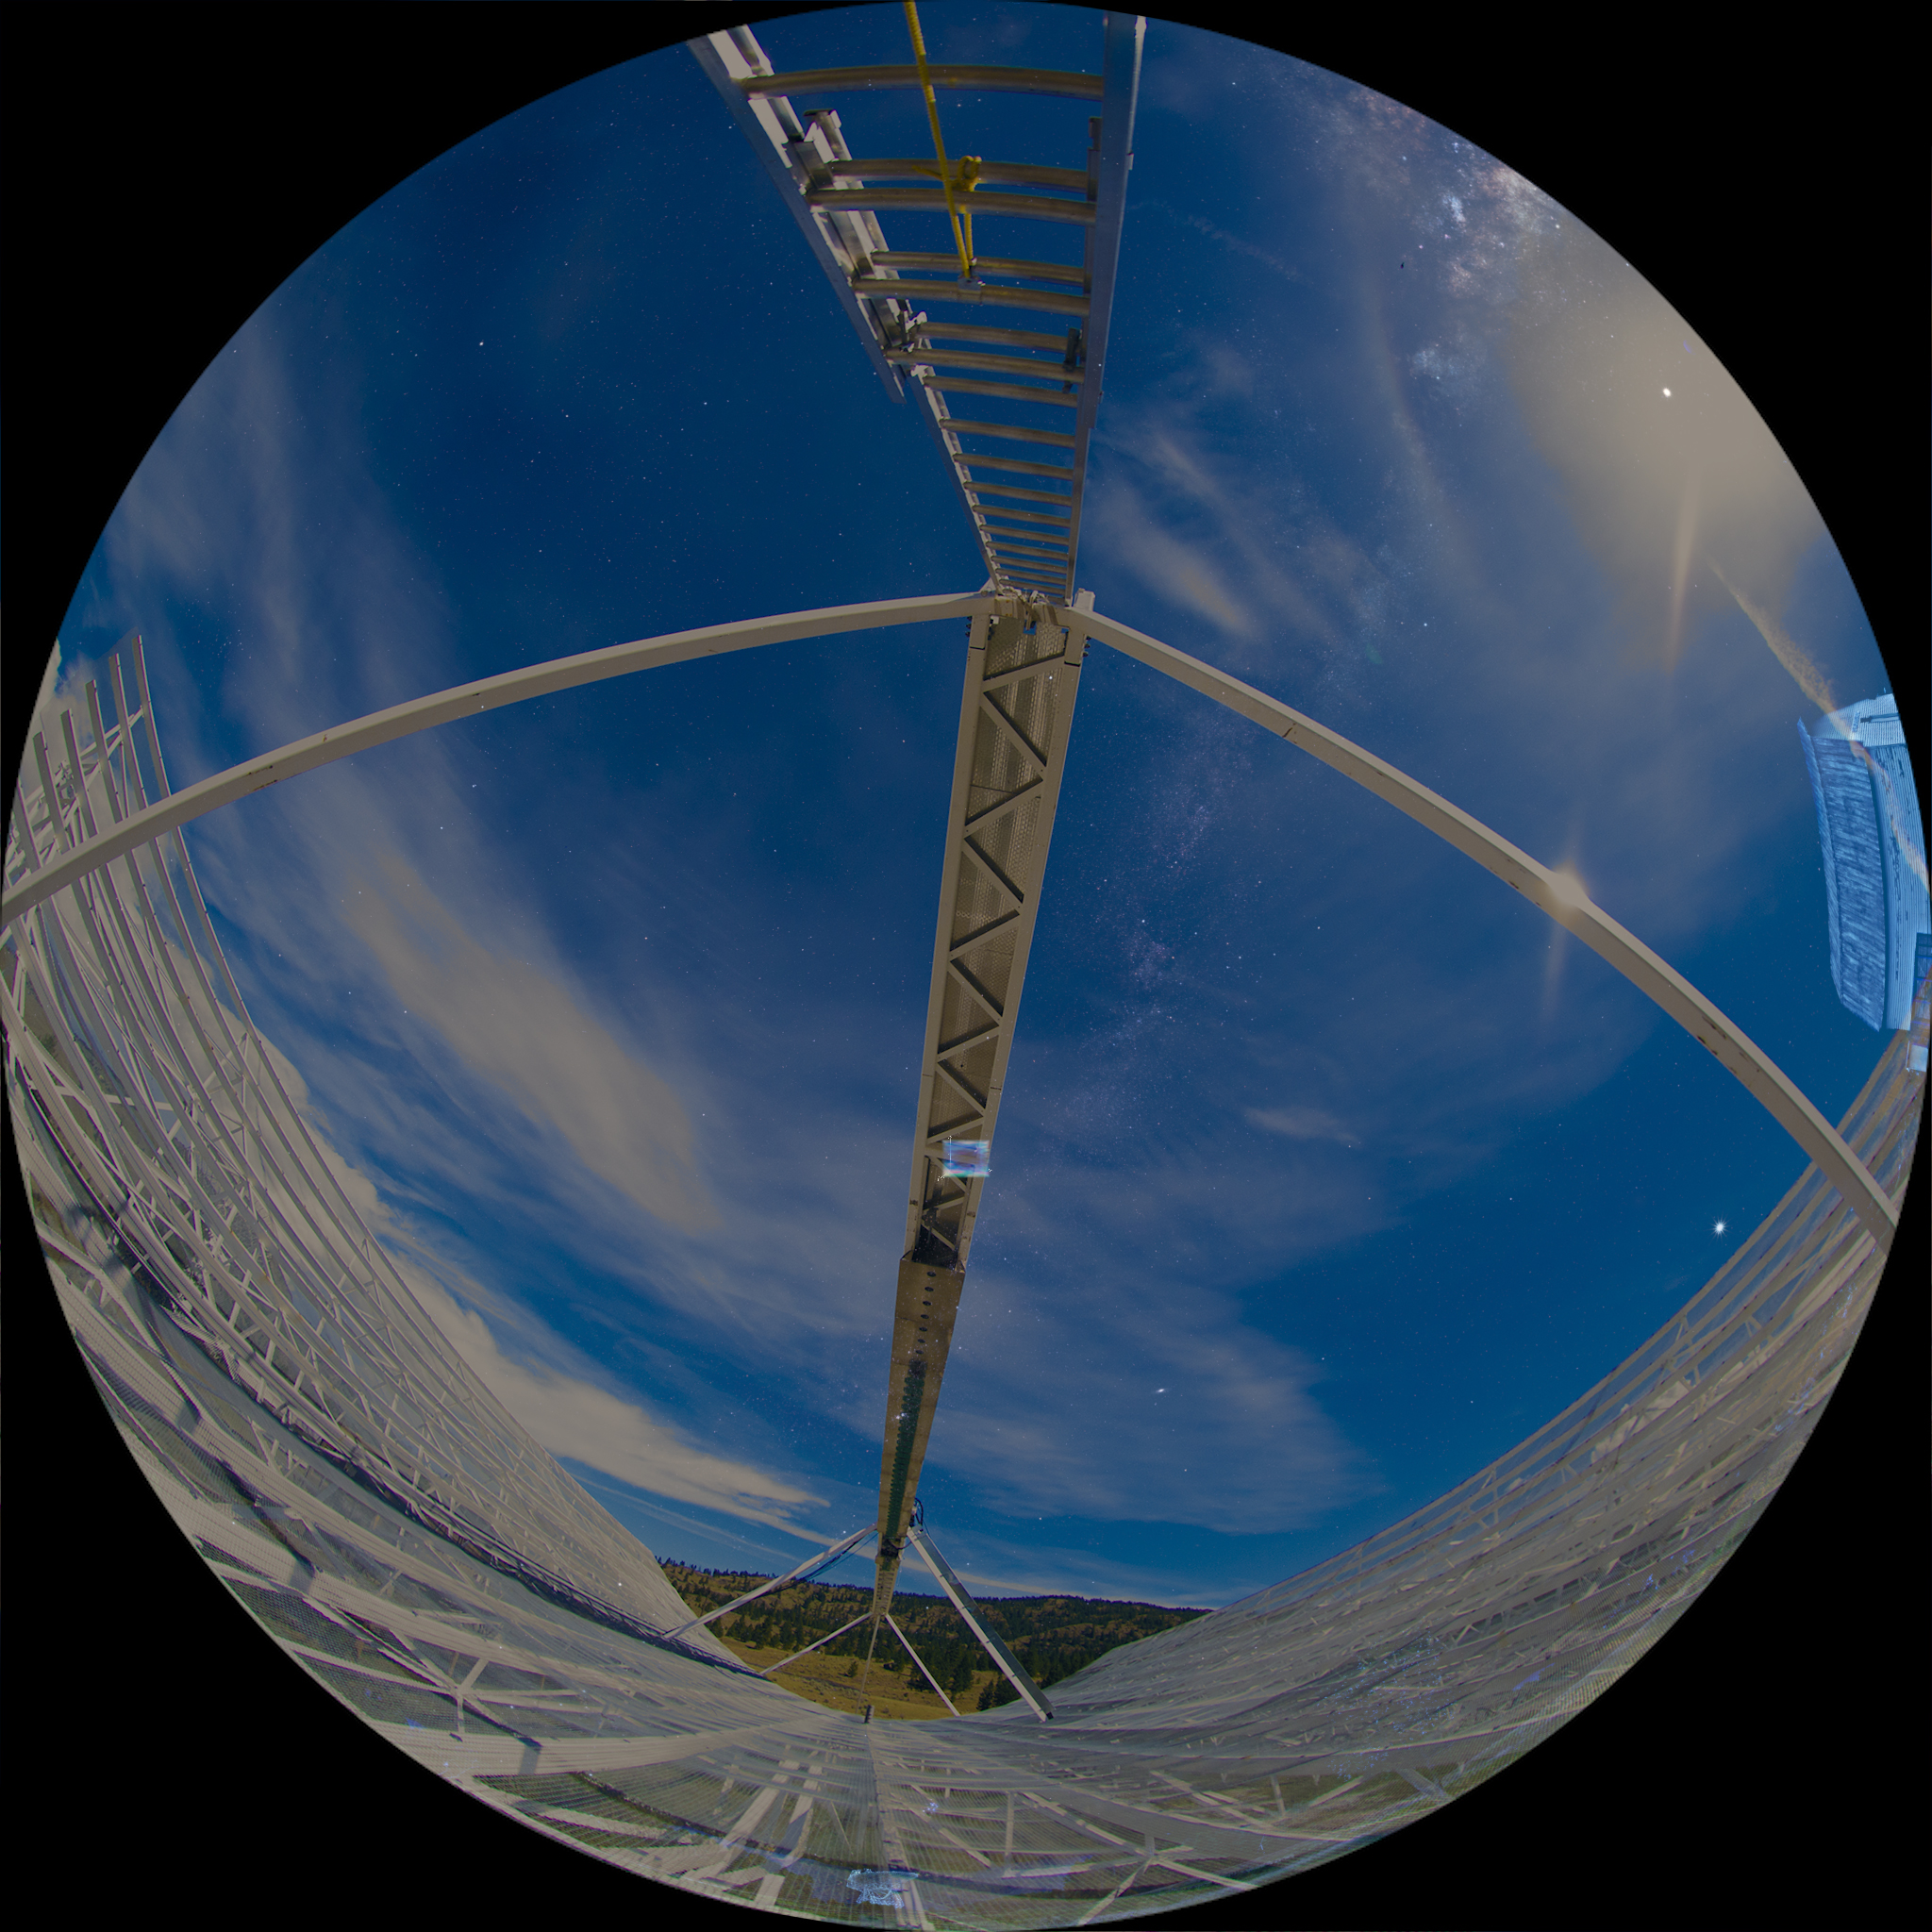
\includegraphics[width=0.3\textwidth]{Planetarium/figures/script_shots/shot28.jpg}} \vspace{0.1cm}\\

\hline

\textit{Located at the Dominion Radio Astrophysical Observatory, near Penticton in British Columbia, Canada; CHIME has cylinders instead of a single, large dish. }& 

\raisebox{-\totalheight}{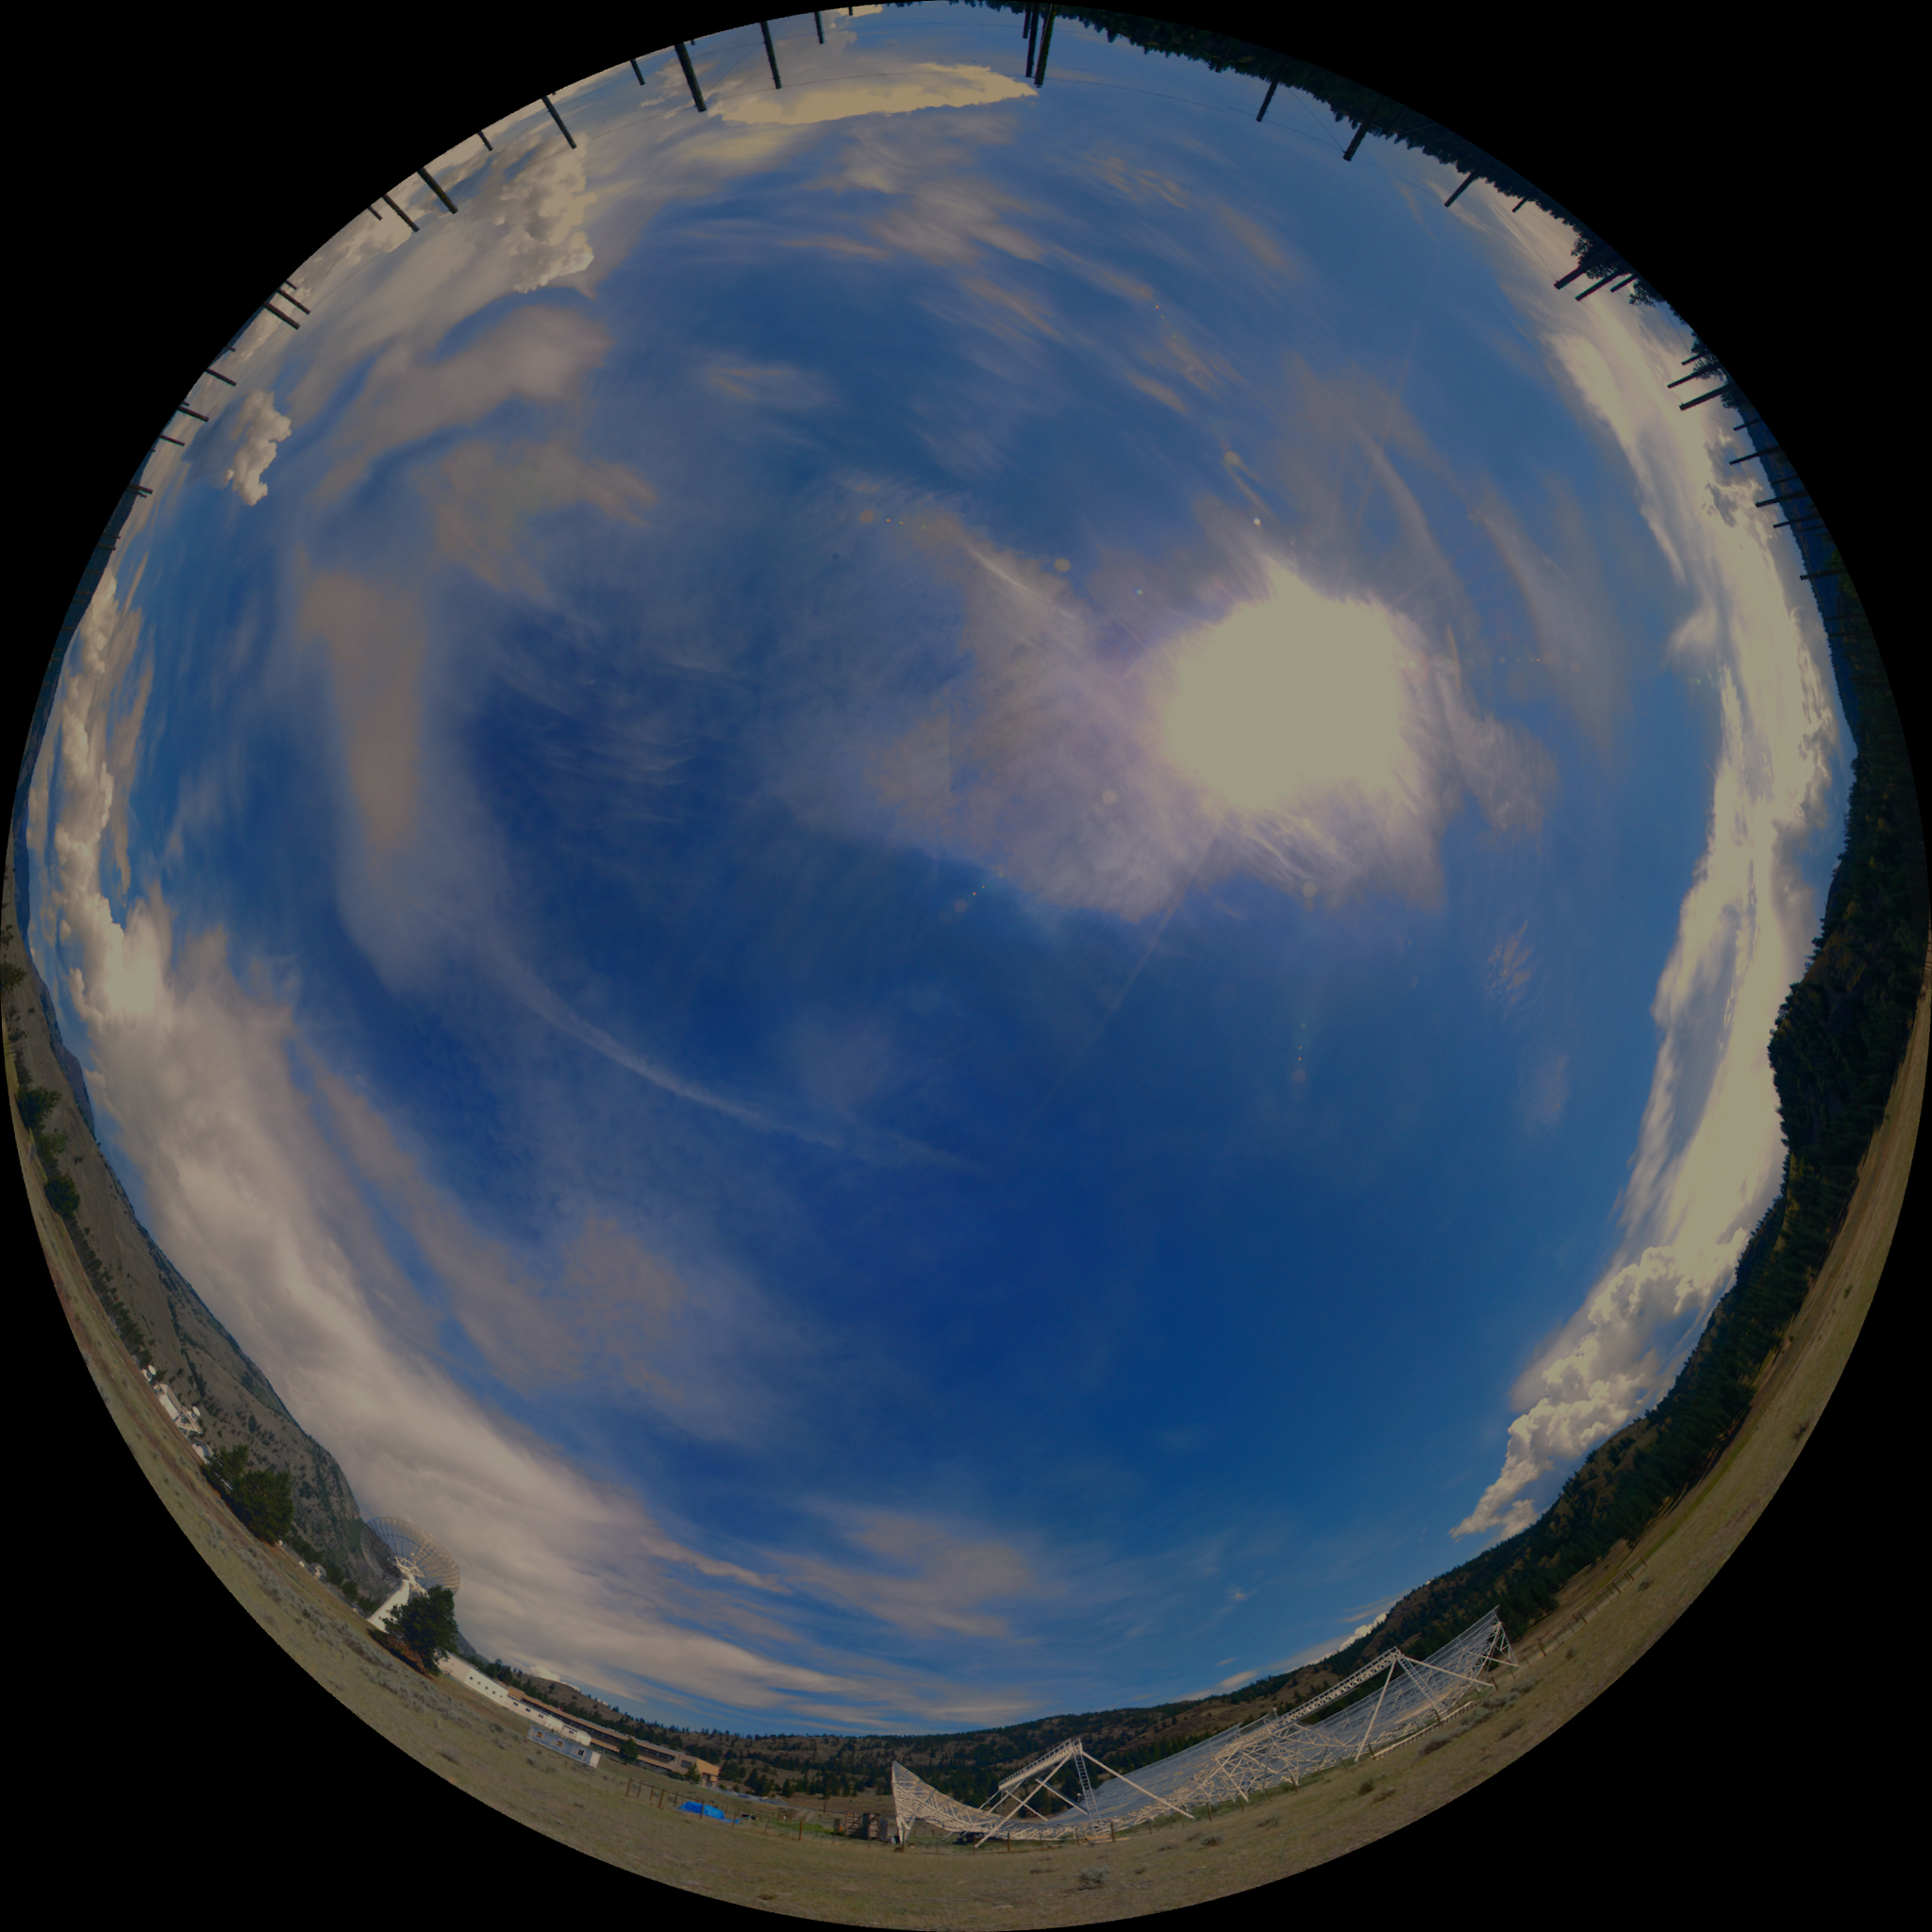
\includegraphics[width=0.3\textwidth]{Planetarium/figures/script_shots/shot29.jpg}} \vspace{0.1cm}\\

\hline

\textit{With many receivers along the center line of each cylinder, CHIME collects light from a stripe of the sky instead of a single point.} &

\raisebox{-\totalheight}{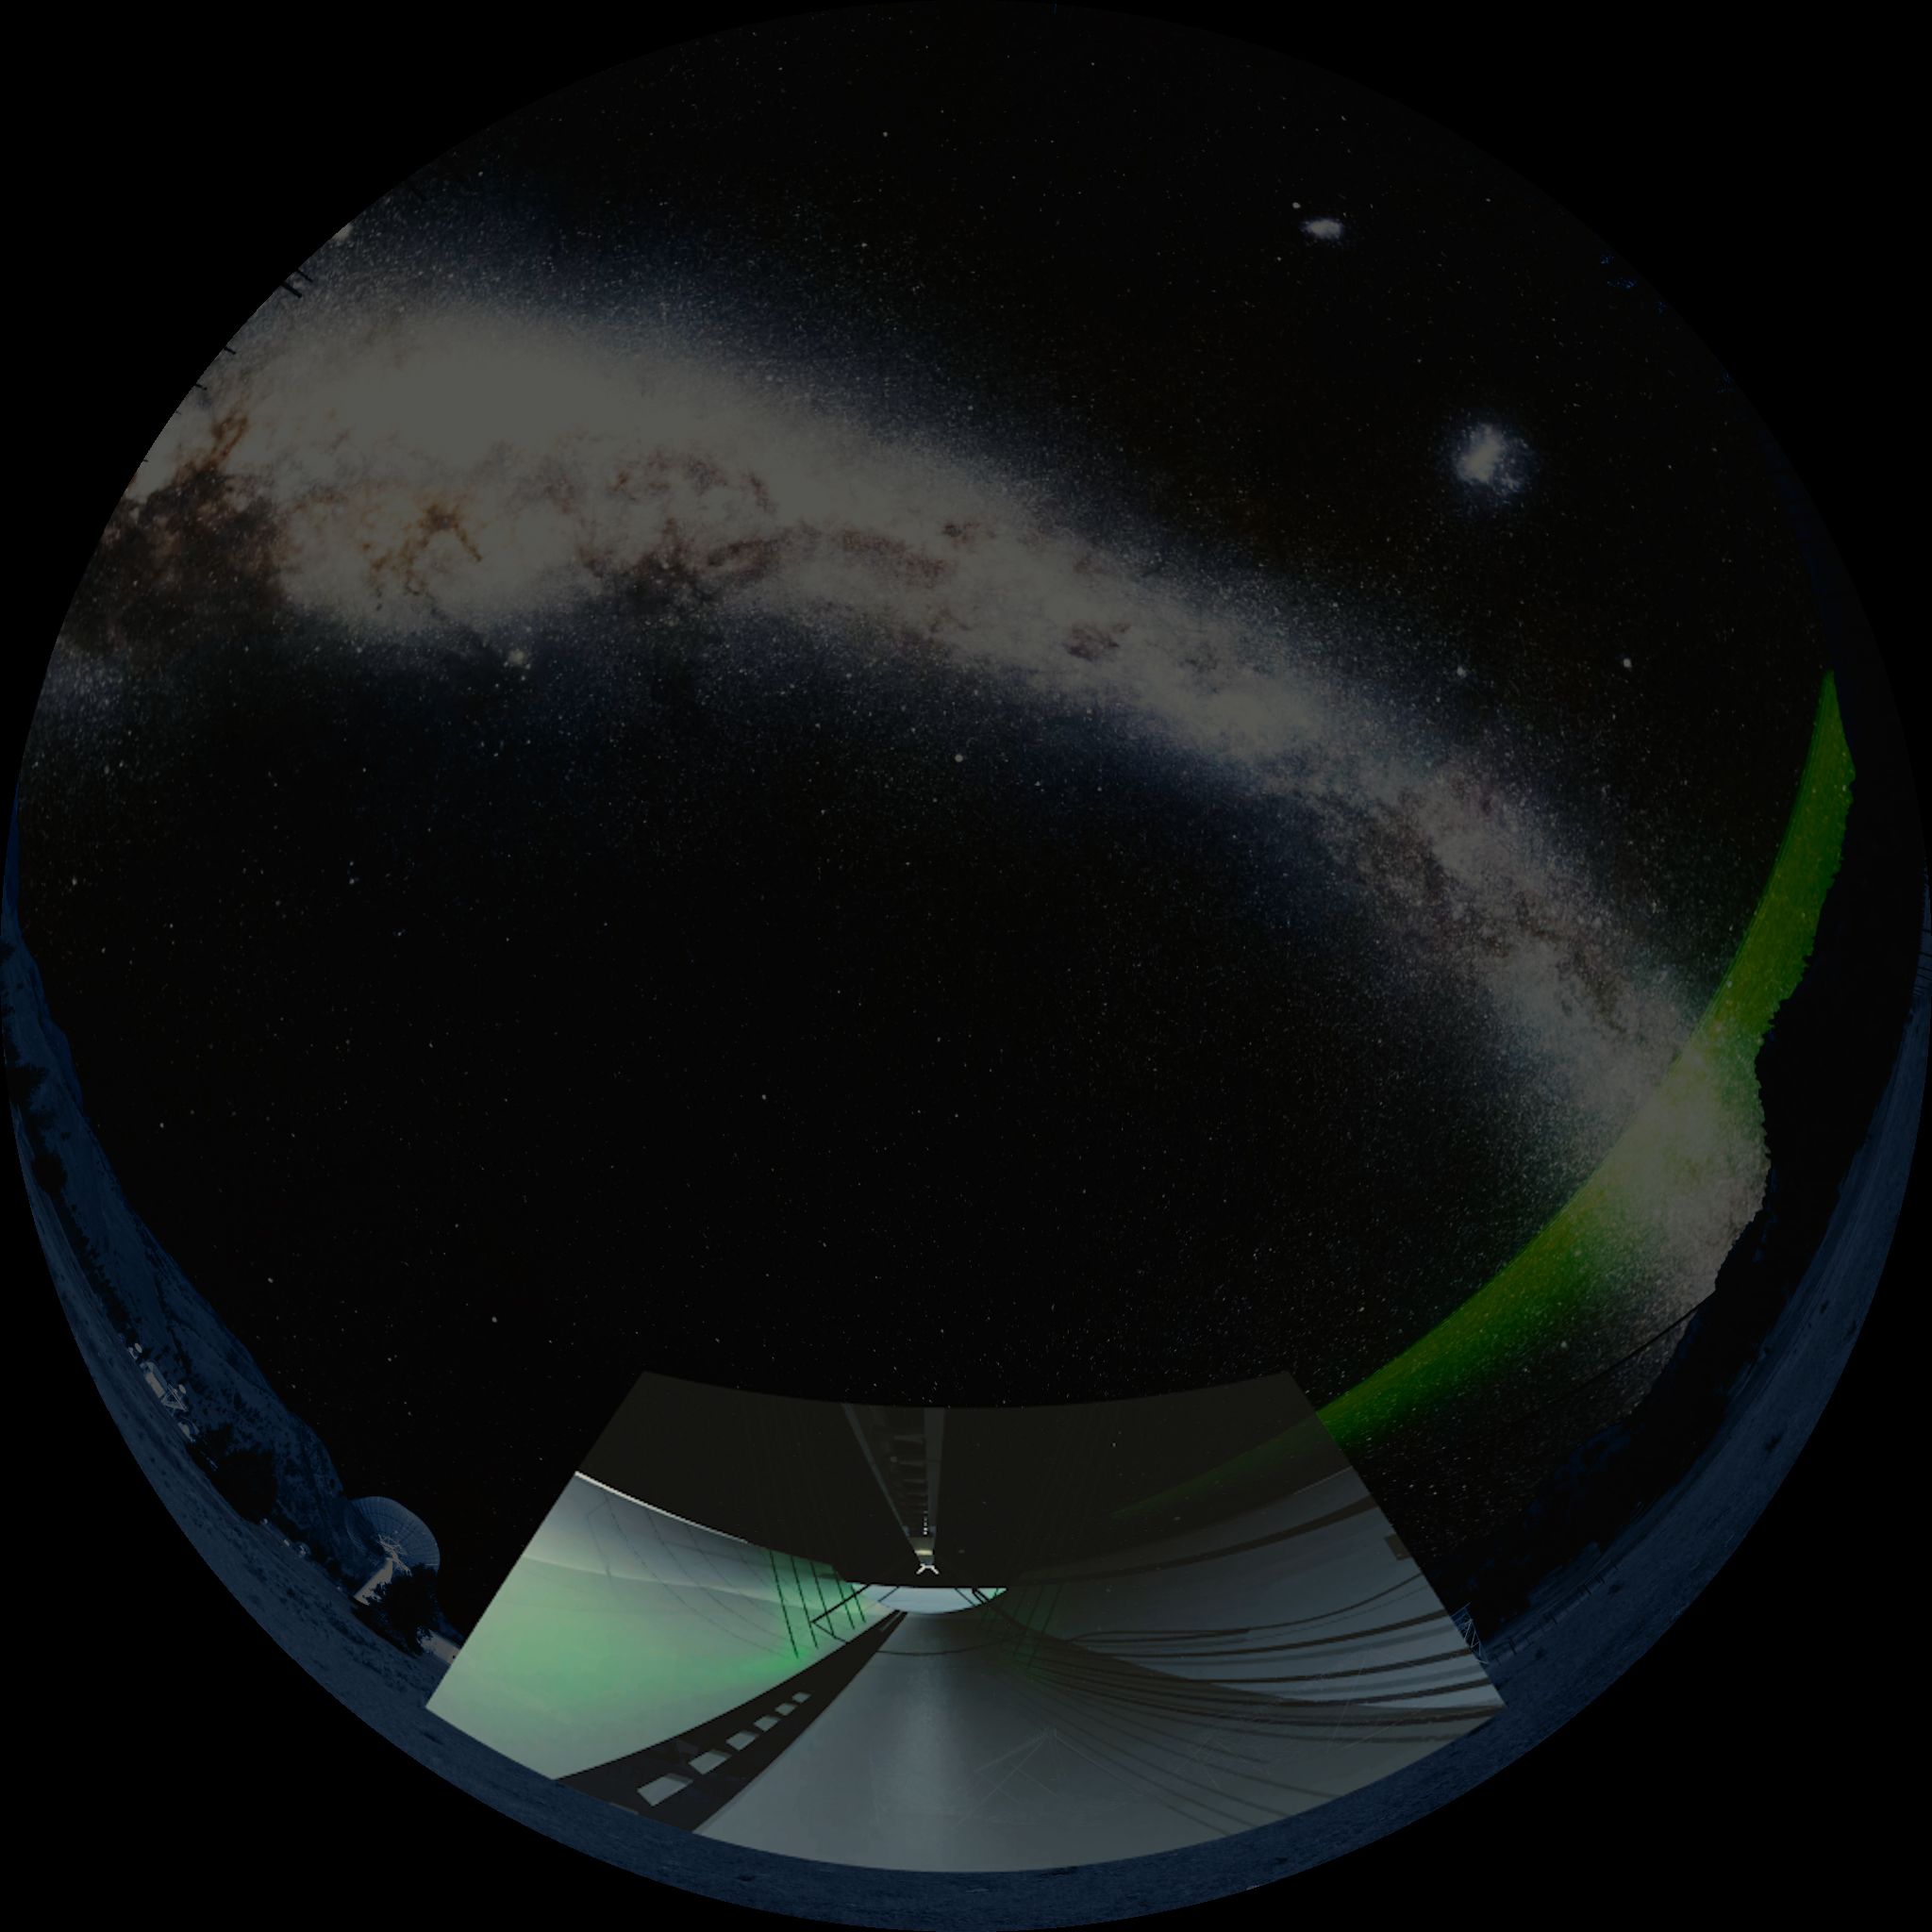
\includegraphics[width=0.3\textwidth]{Planetarium/figures/script_shots/shot30.jpg}} \vspace{0.1cm}\\

\hline

\textit{Meanwhile, the rotation of the Earth causes the cylinder to see a slightly different stripe of sky each second.} & 

\raisebox{-\totalheight}{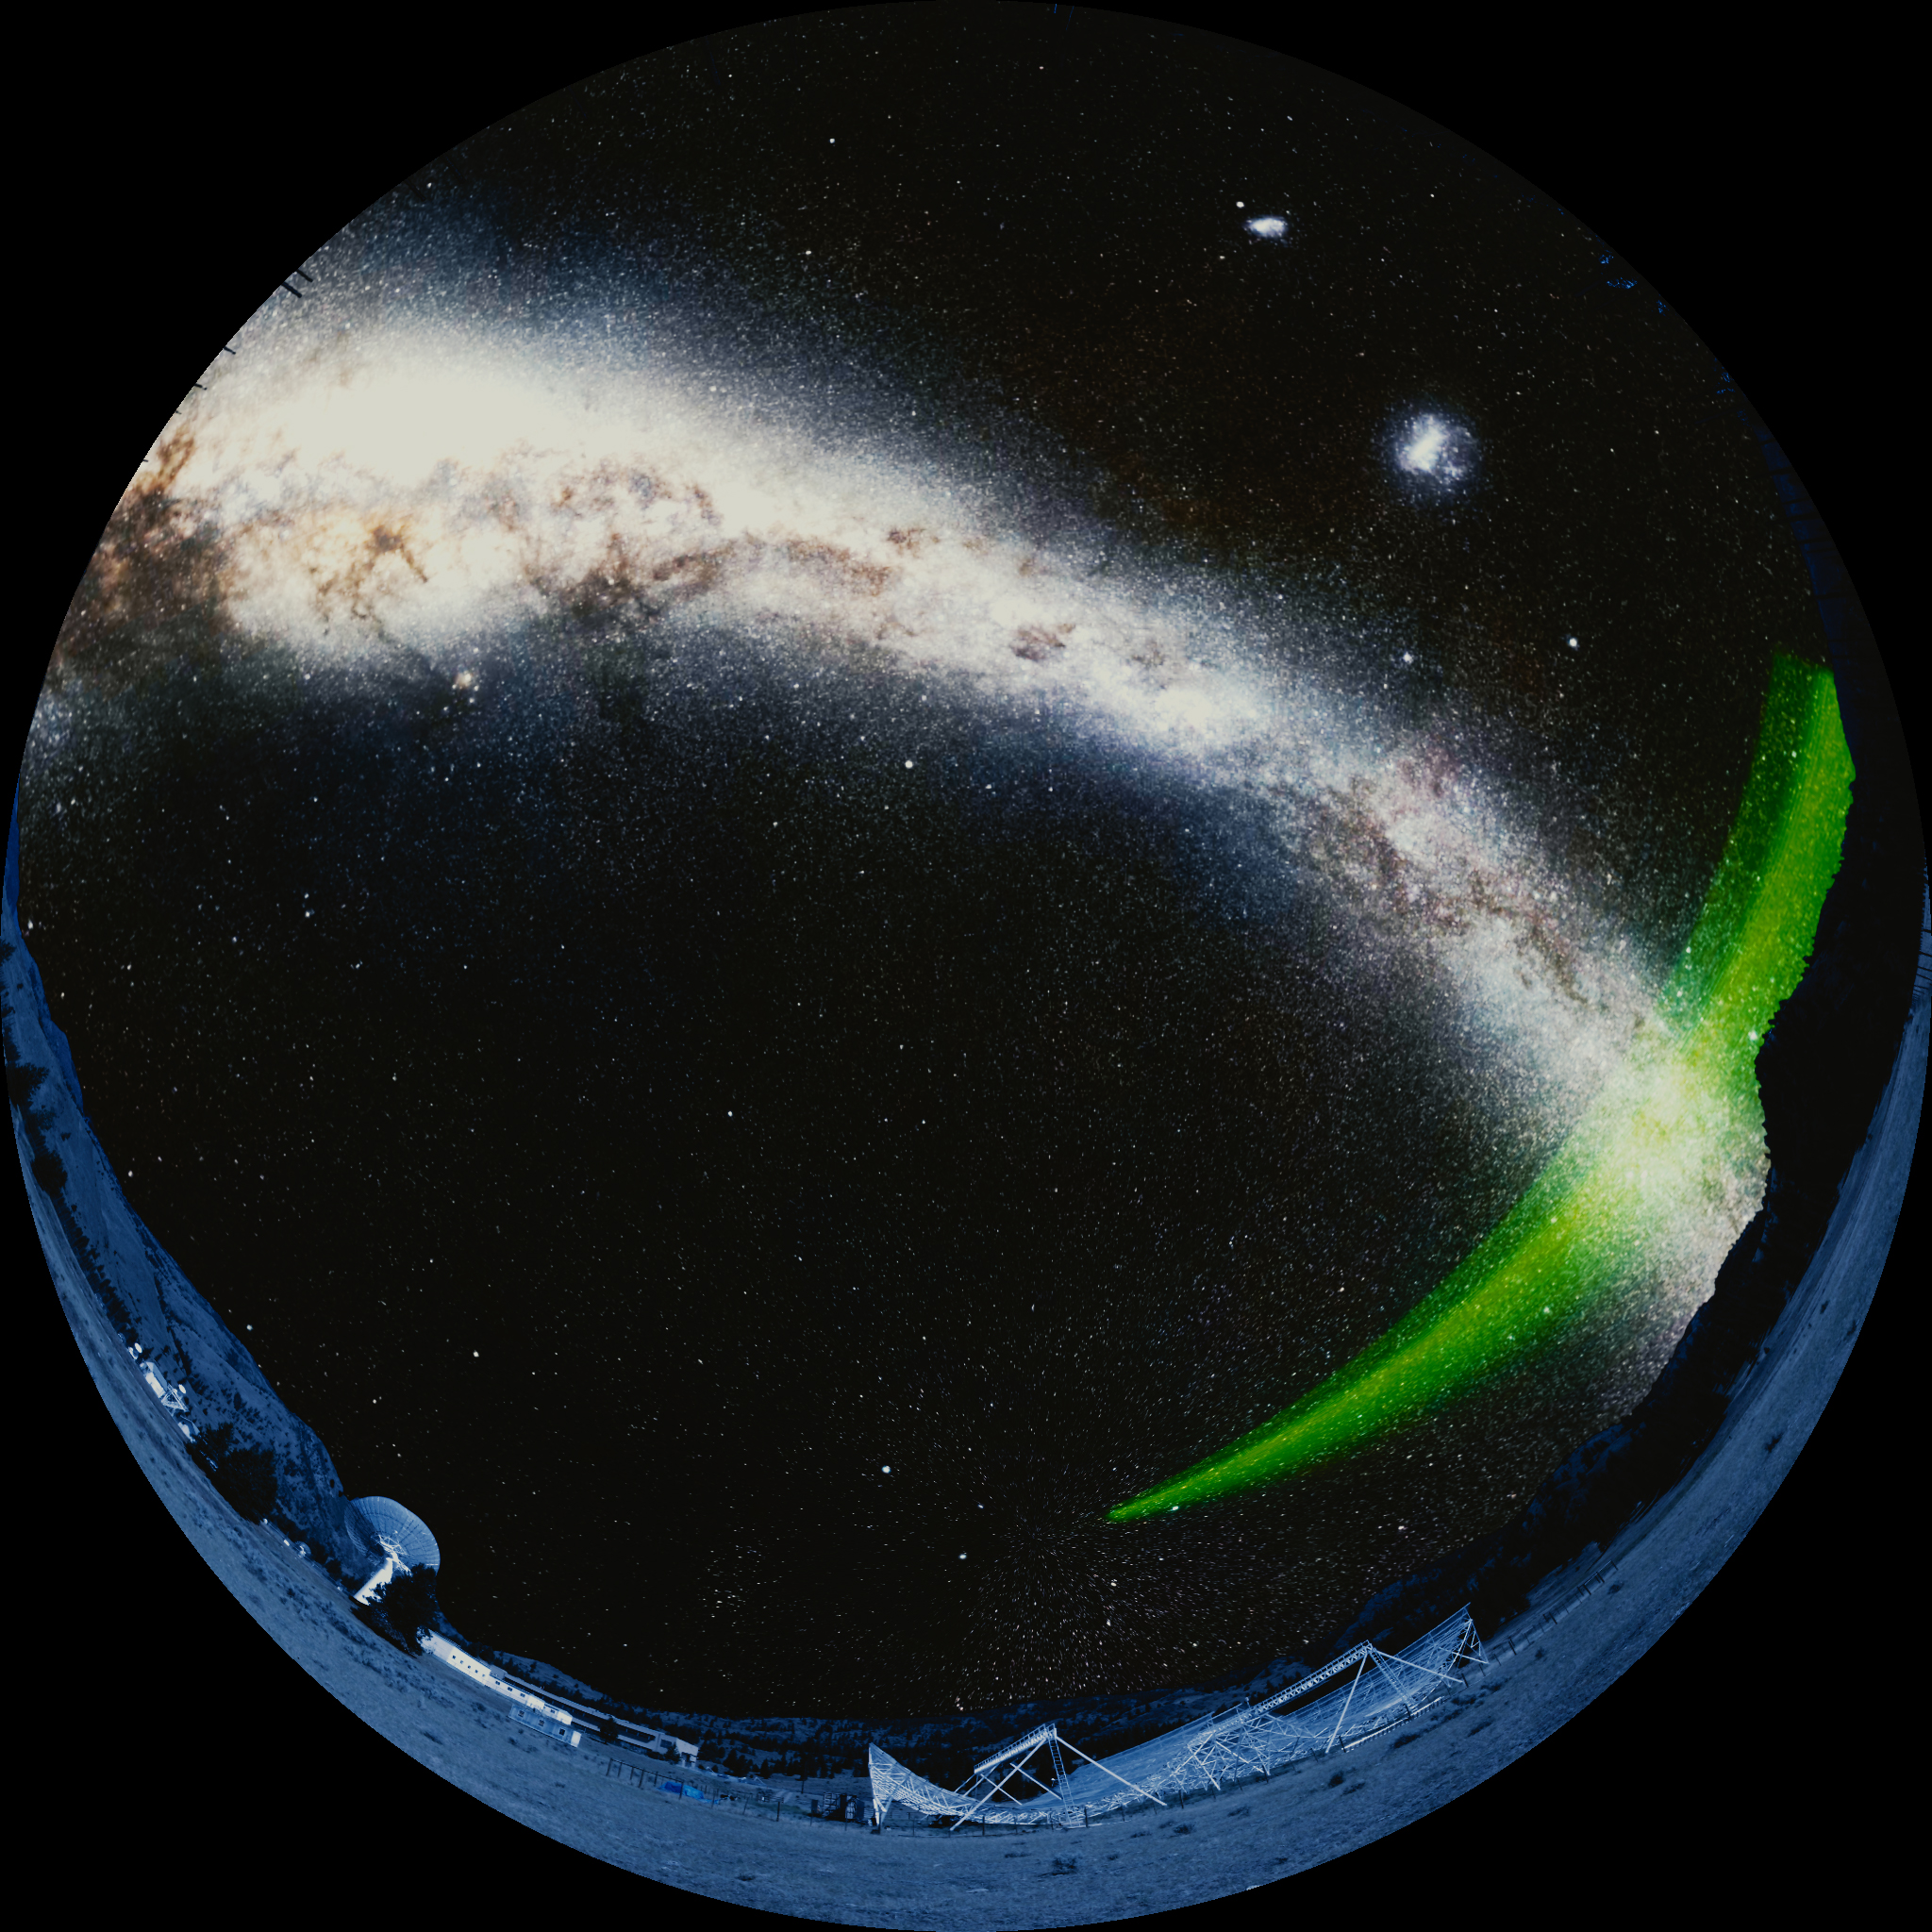
\includegraphics[width=0.3\textwidth]{Planetarium/figures/script_shots/shot31.jpg}} \vspace{0.1cm}\\

\hline

\textit{During the course of a day, photons of light are collected for the entire sky as seen from that location; which is about half the overall sky. So maps of the Hydrogen sky can now be made much more quickly than with the Green Bank Telescope. }& 

\raisebox{-\totalheight}{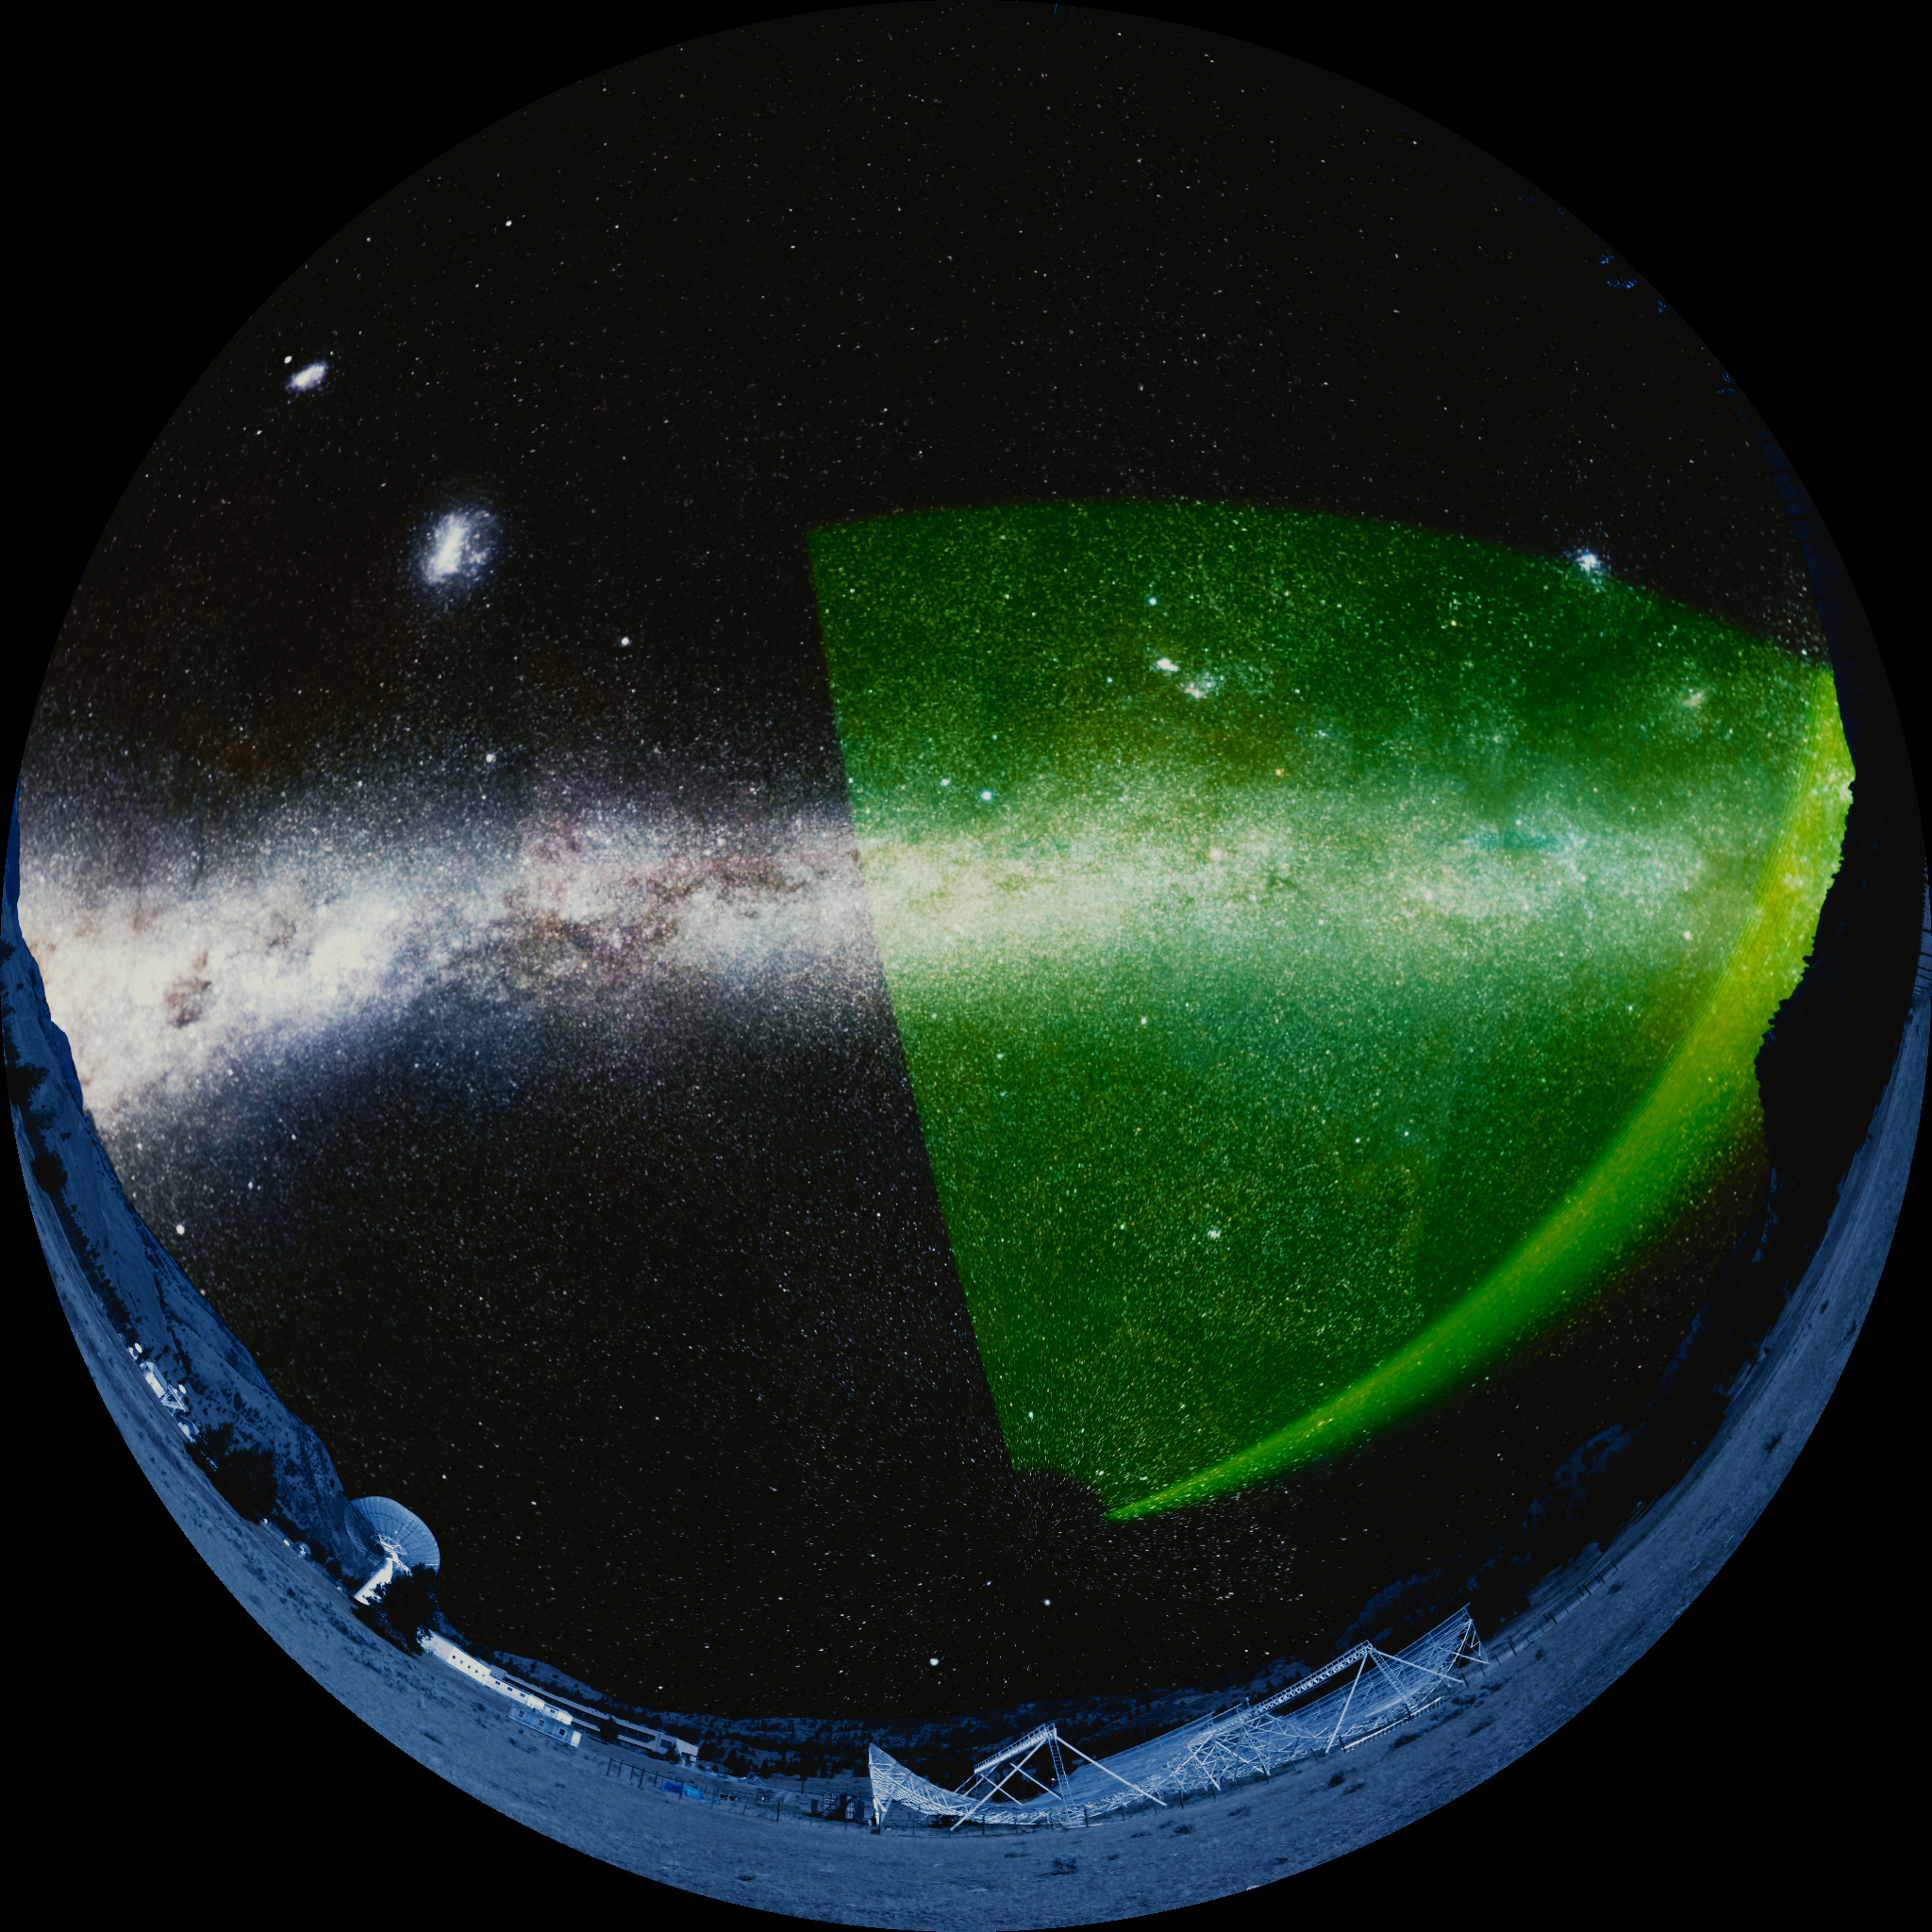
\includegraphics[width=0.3\textwidth]{Planetarium/figures/script_shots/shot32.jpg}} \vspace{0.1cm}\\
 
\hline

\textit{In the future, we will use the maps of the Hydrogen sky in combination with observations from other telescopes to fill in gaps in our picture of the universe. }& 

\raisebox{-\totalheight}{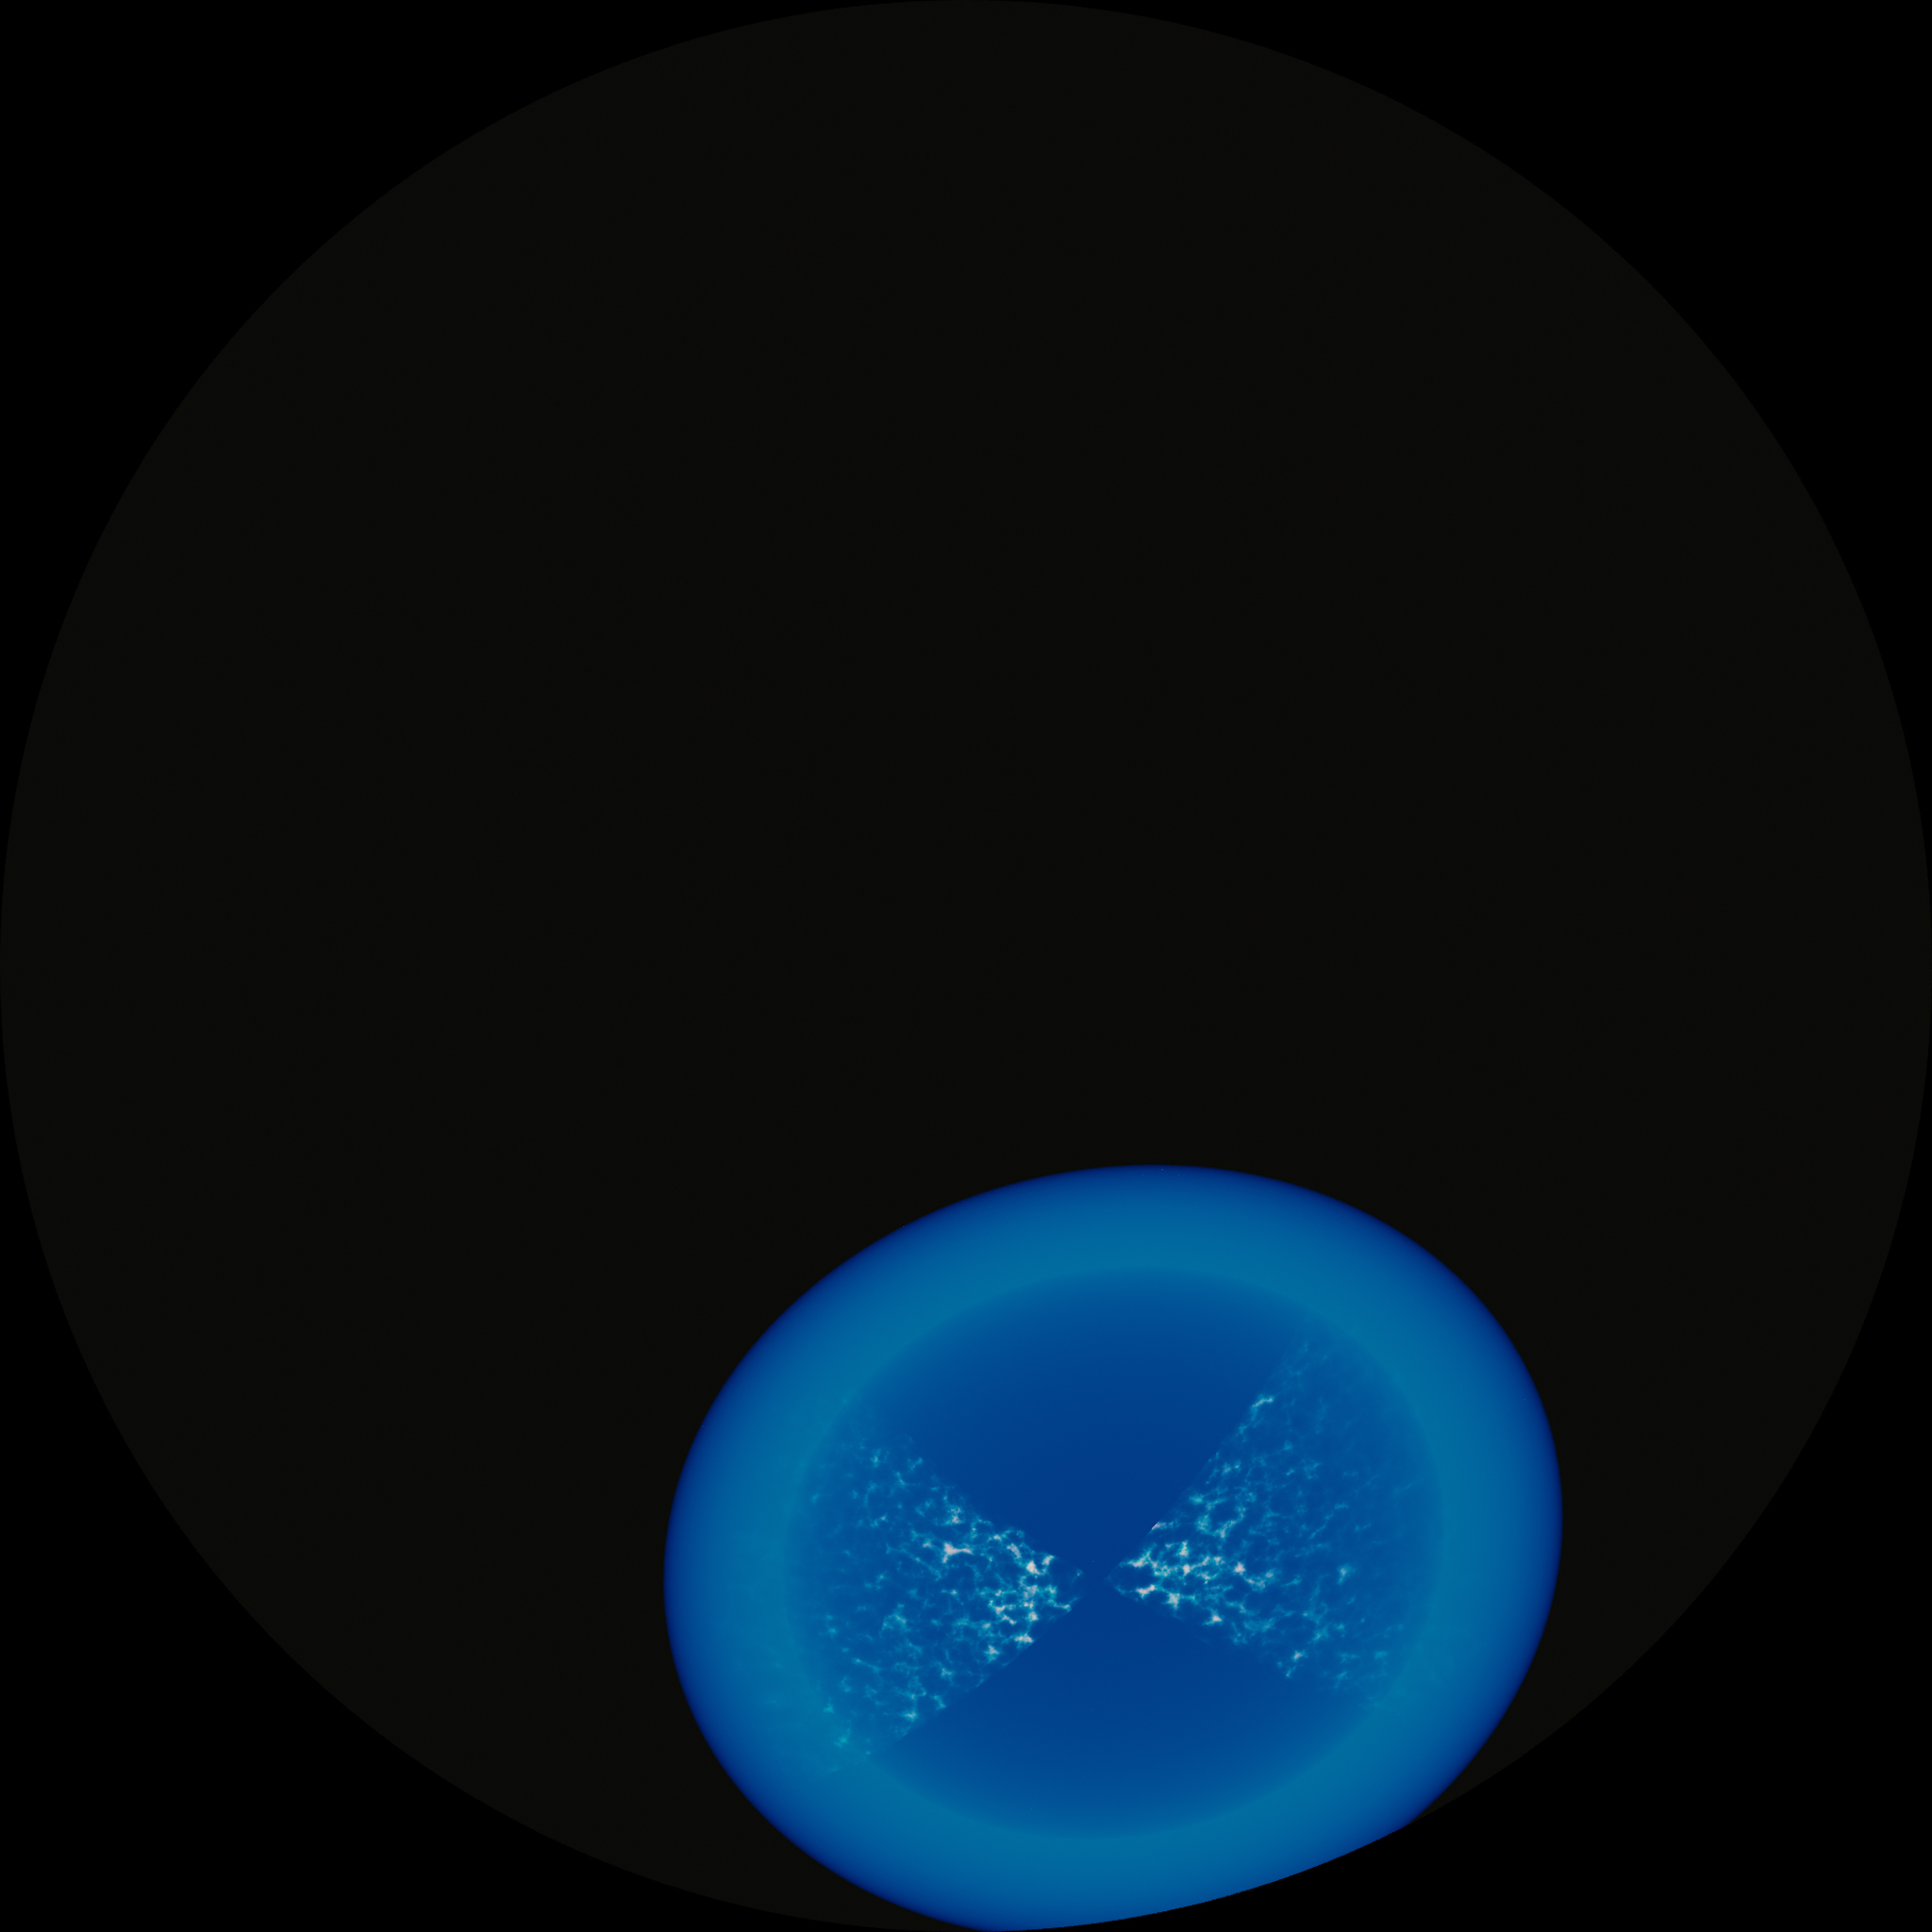
\includegraphics[width=0.3\textwidth]{Planetarium/figures/script_shots/shot33.jpg}} \vspace{0.1cm}\\

\hline

\textit{This will allow us to study many things including the basic building blocks of the universe, young galaxies, and even the first stars in the universe; which lived and died before the Earth existed. }& 

\raisebox{-\totalheight}{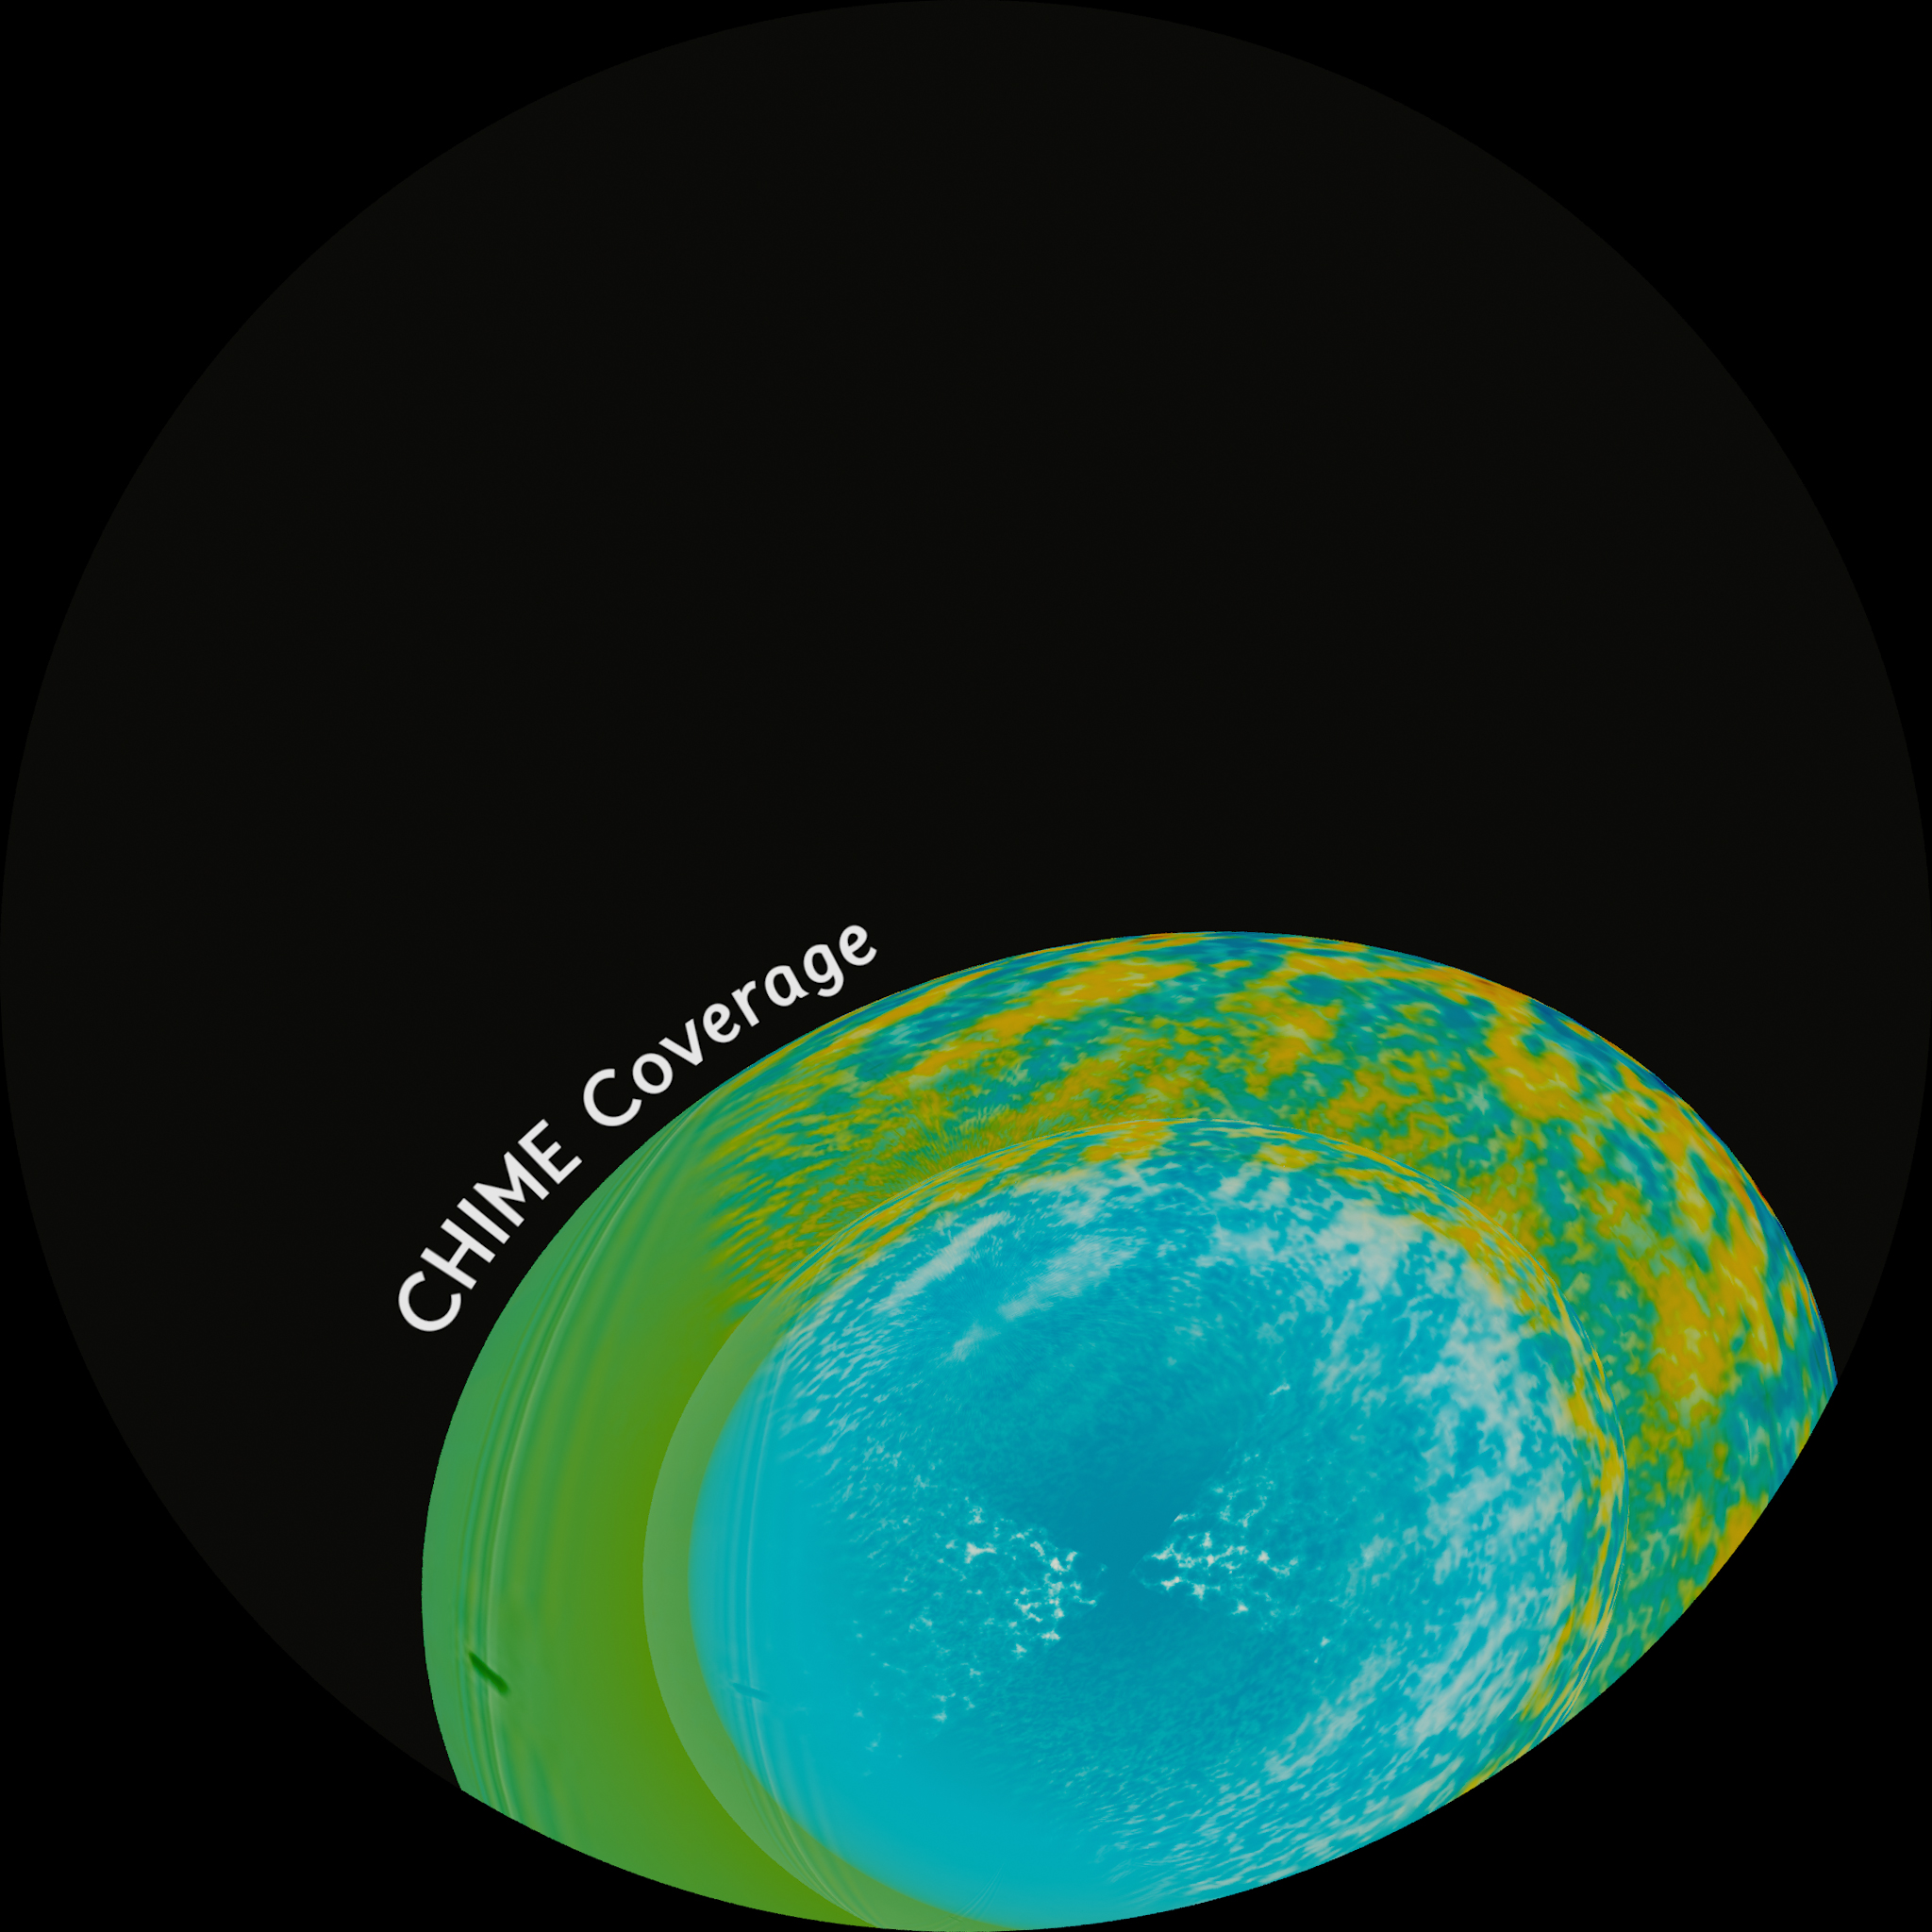
\includegraphics[width=0.3\textwidth]{Planetarium/figures/script_shots/shot34.jpg}} \vspace{0.1cm}\\

\hline

\textit{Because there are so many interesting scientific applications for the Hydrogen sky, new radio telecopes such as CHIME are currently under development around the world. With these new telescopes the future is bright for the Hydrogen sky. }& 

\raisebox{-\totalheight}{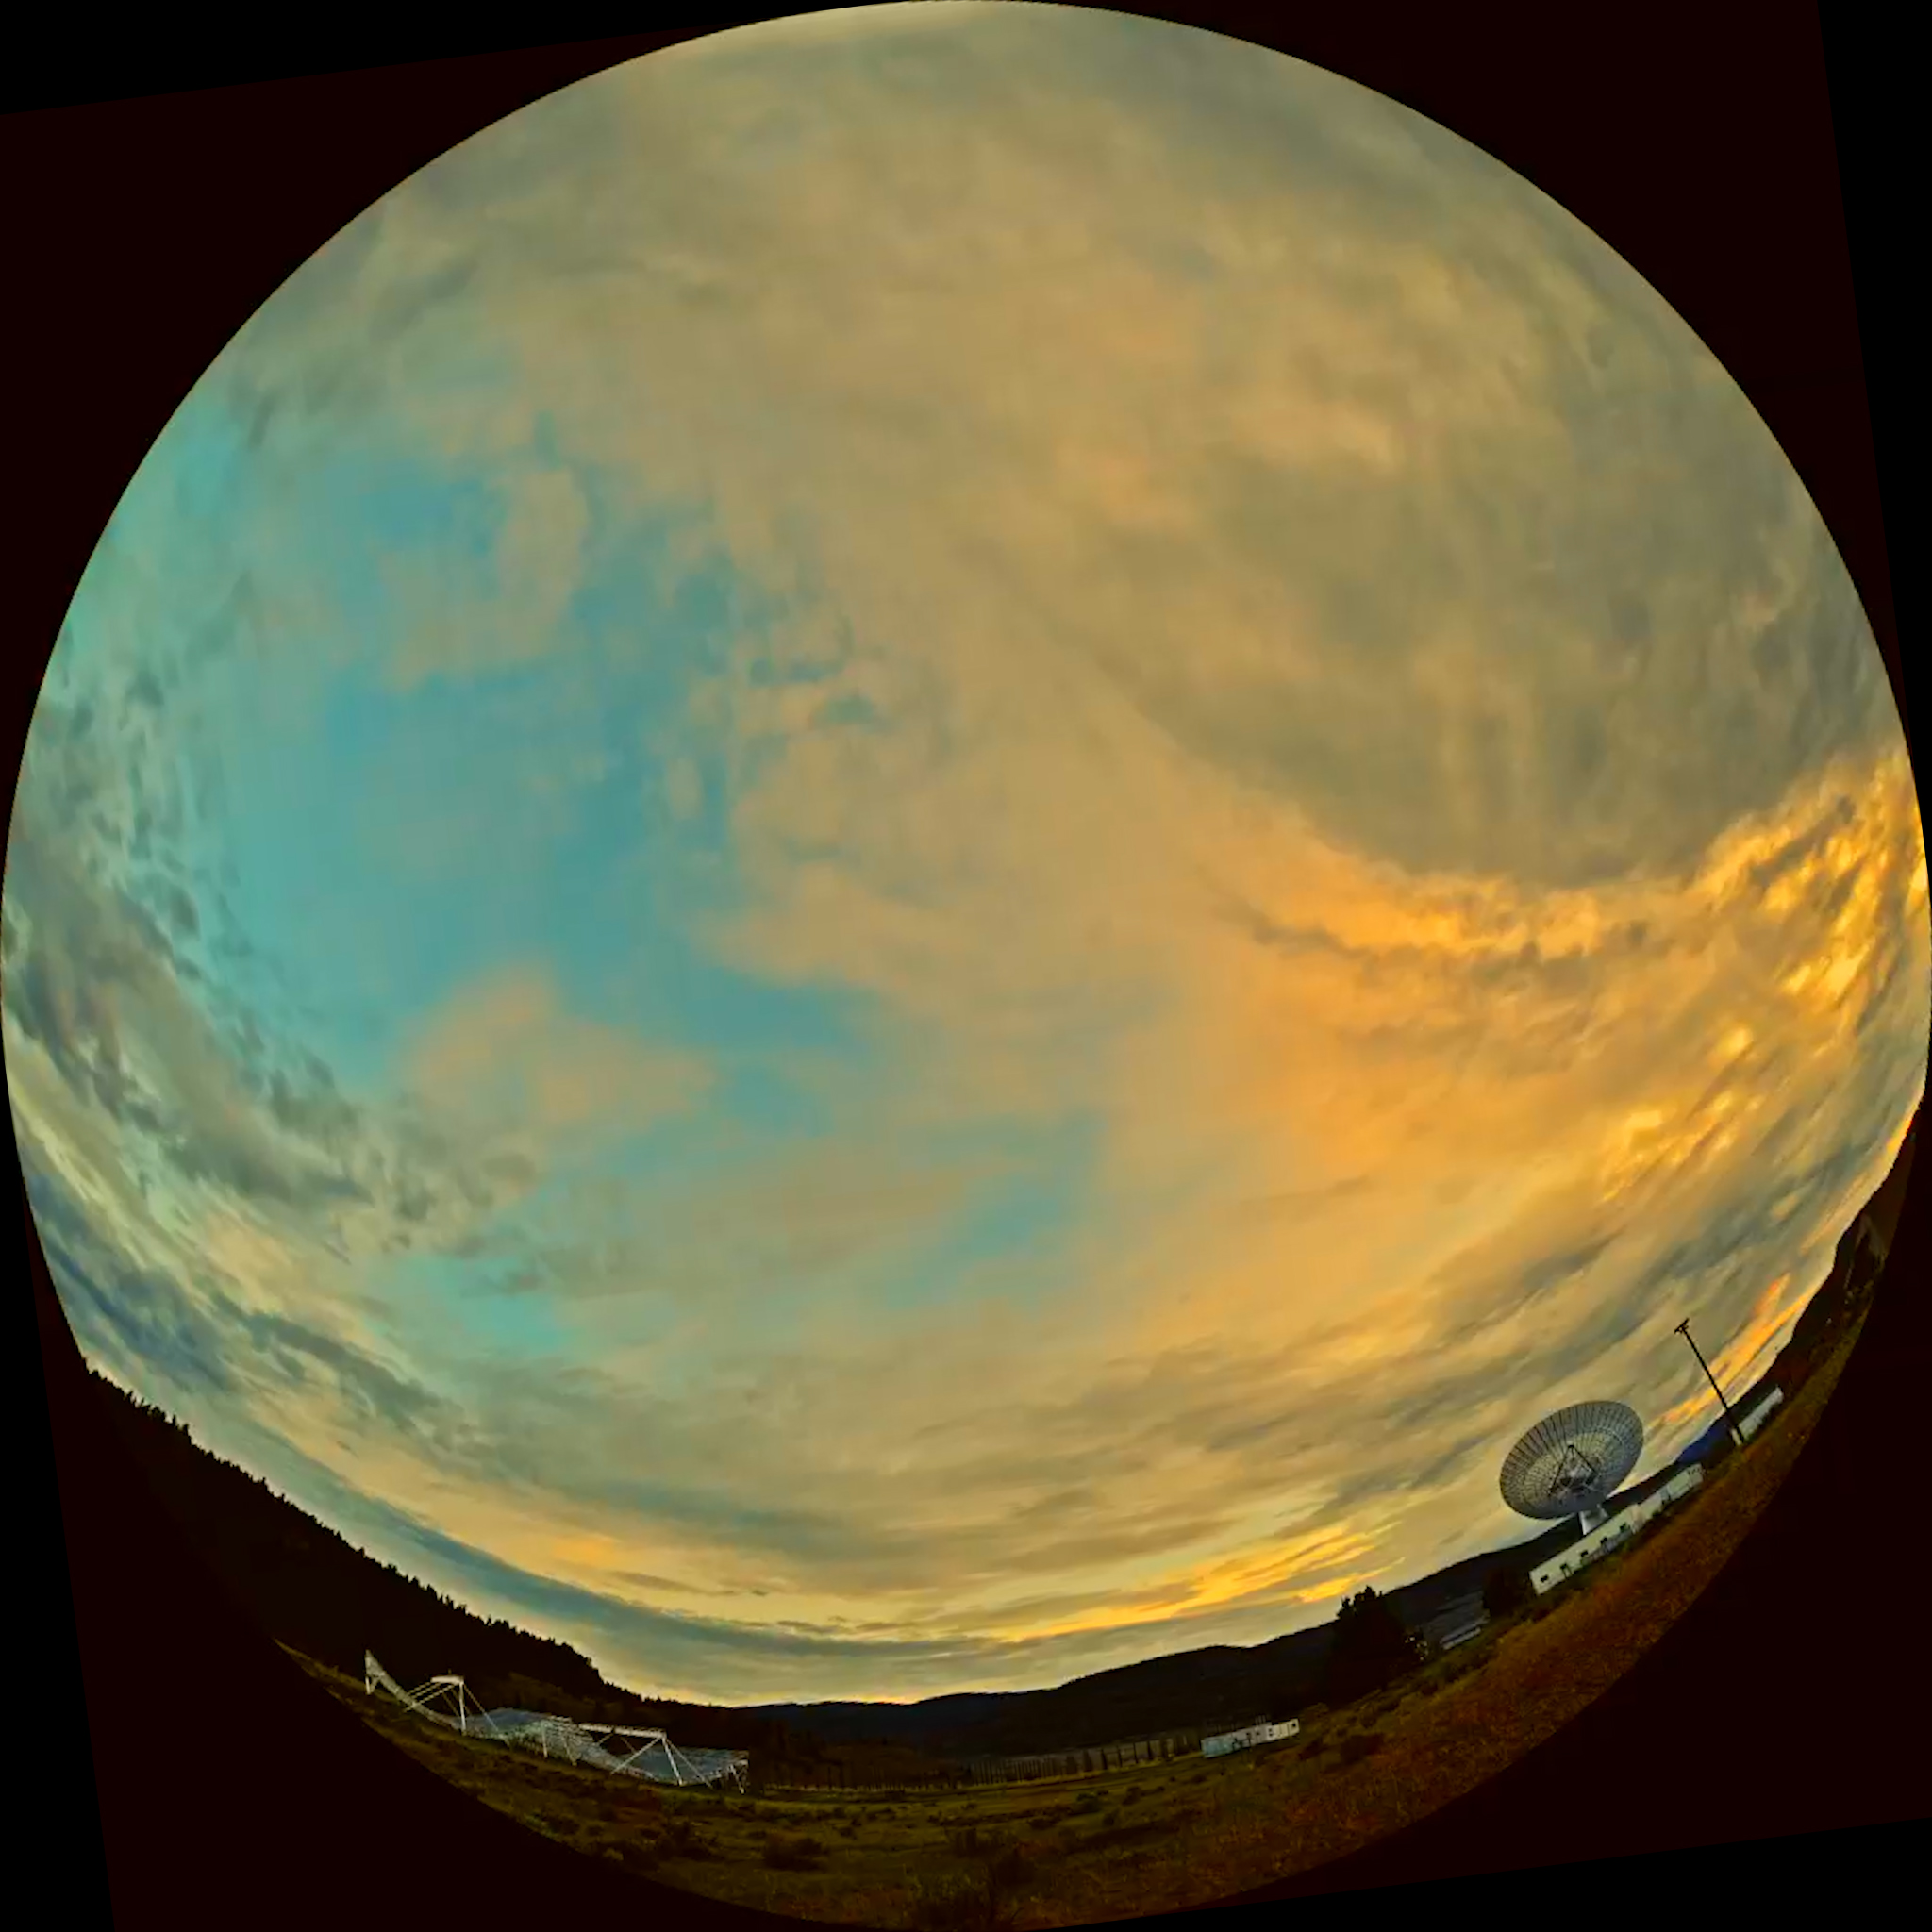
\includegraphics[width=0.3\textwidth]{Planetarium/figures/script_shots/shot35.jpg}} \vspace{0.1cm}\\

\hline

\end{longtable}
%\end{table}
\end{center}



\section{On-site Filming}

One of the key components of this show was on-site filming at a couple of real radio telescopes, the Robert C. Byrd Green Bank Radio Telescope (GBT)\footnote{\url{https://science.nrao.edu/facilities/gbt/}} and the Canadian Hydrogen Intensity Mapping Experiment (CHIME)\footnote{\url{http://chime.phas.ubc.ca/}}. For filming, we focused on still images and time lapses rather than video footage. We found that video footage did not translate well into the dome environment, as any irregular motion in the videos was magnified by the shape of the dome.  

We used two Nikon DSLR cameras (an old D80 and a new D800), with a rectangular lens on the D80 and a circular fisheye lens on the D800. The D80 was used primarily to capture images for creating panoramas of the locations we visited, while the fisheye was used for capturing single images and doing time-lapse videos. 

\begin{figure}[htb]
\centering
\begin{minipage}[b]{0.39\textwidth}
\centering
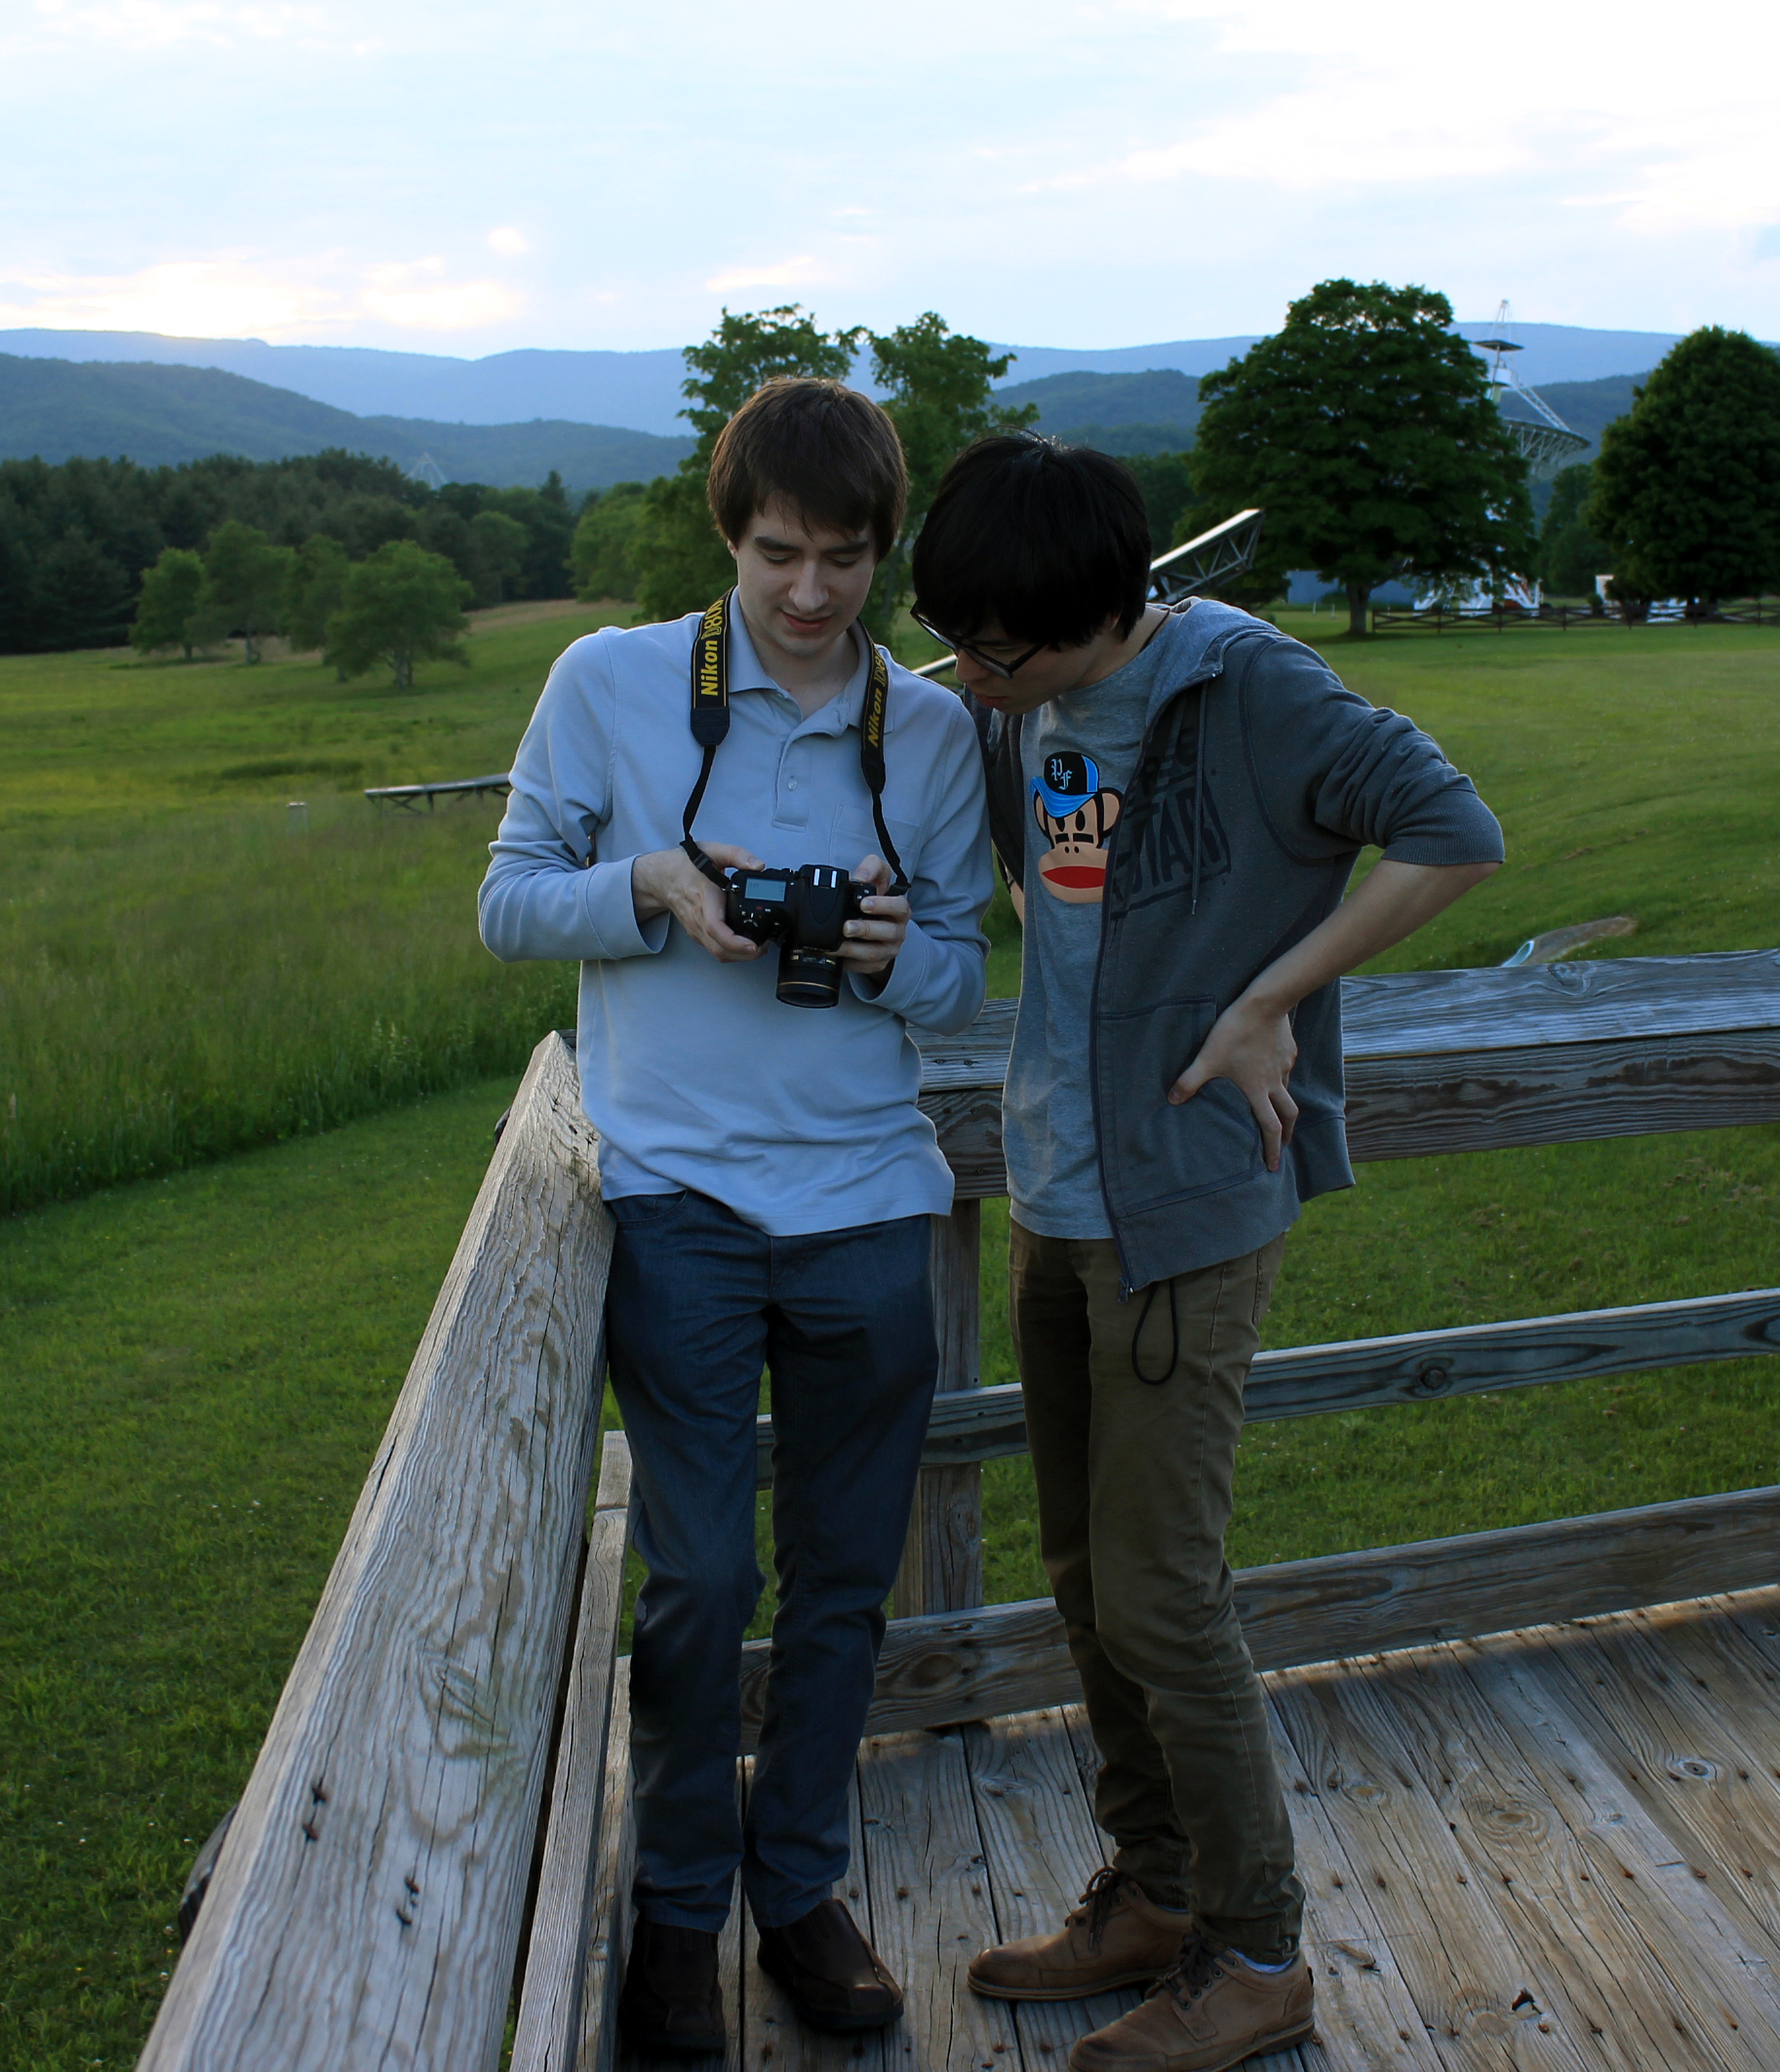
\includegraphics[width=0.95\linewidth]{Planetarium/figures/Filming_at_GBT_obs_deck.jpg}
\caption{Alex and Meng checking an image during filming.}
\label{Fig:GBT_obs_deck_film}
\end{minipage}%
\begin{minipage}[b]{0.02\textwidth}
\hspace{1cm}
\end{minipage}%
\begin{minipage}[b]{0.55\textwidth}
\centering
\includegraphics[width=0.95\linewidth]{Planetarium/figures/Filming_at_GBT_telescope_base.jpg}
\caption{Alex, Meng and Hsiu-Hsien taking multiple shots of the GBT from its base.}
\label{Fig:GBT_base_film}
\end{minipage}
\end{figure}

\begin{figure}[htb]
\centering
\begin{minipage}[b]{0.53\textwidth}
\centering
\includegraphics[width=0.95\linewidth]{Planetarium/figures/GBT_control_room.jpg}
\caption{Some of the monitors in the GBT control room, captured with the rectangular lens. }
\label{Fig:GBT_control}
\end{minipage}%
\begin{minipage}[b]{0.02\textwidth}
\hspace{1cm}
\end{minipage}%
\begin{minipage}[b]{0.43\textwidth}
\centering
\includegraphics[width=0.95\linewidth]{Planetarium/figures/GBT_dusk.jpg}
\caption{GBT as seen from the observation deck, captured with the rectangular lens.}
\label{Fig:GBT_dusk}
\end{minipage}
\end{figure}

\begin{figure}[htb]
%\begin{center}
\centering
\begin{minipage}[b]{0.54\textwidth}
\centering
\includegraphics[width=0.95\linewidth]{Planetarium/figures/GBT_dusk_fisheye.jpg}
\caption{GBT as seen from the observation deck, captured with the fisheye lens.}
\label{Fig:GBT_dusk_fisheye}
\end{minipage}%
\begin{minipage}[b]{0.02\textwidth}
\hspace{1cm}
\end{minipage}%
\begin{minipage}[b]{0.42\textwidth}
\centering
%\end{center}
%\end{figure}
%\begin{figure}[htb]
%\begin{center}
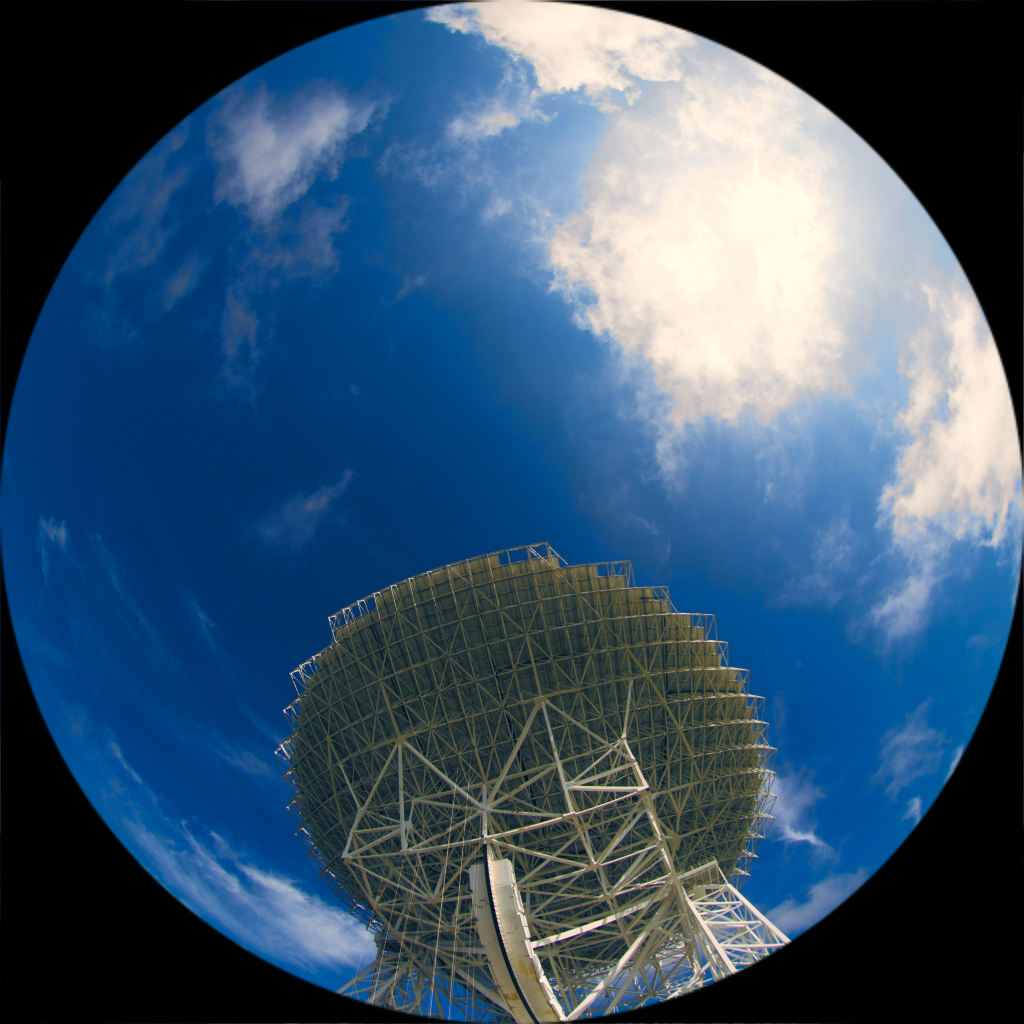
\includegraphics[width=0.95\linewidth]{Planetarium/figures/GBT_base_render.jpg}
\caption{GBT as seen from its base, composited from images with the fisheye lens.}
\label{Fig:GBT_base_fisheye}
%\end{center}
\end{minipage}
\end{figure}


\subsection{Green Bank, WV}

I visited the National Radio Astronomy Observatory (NRAO) Green Bank site twice to gather footage in June and August 2014. For the June visit, Alex and Meng accompanied me to the site. We were able to stay on-site at the telescope and get footage both from the general site and from up close to the main $100 m$ Green Bank Telescope. Footage had to be collected during the telescope maintenance time, as the cameras are a source of radio frequency interference (RFI) for the telescope when it is actually running.

Mike Holstine, the business manager at the Green Bank site, was our primary contact for the trips. He was able to get us a tour of the Robert C. Byrd Green Bank Radio Telescope, including taking two elevators up to the receiver on top of the telescope. Figures \ref{Fig:GBT_obs_deck_film} and \ref{Fig:GBT_base_film} show us filming at the GBT, while Figures \ref{Fig:GBT_control}, \ref{Fig:GBT_dusk}, \ref{Fig:GBT_dusk_fisheye}, and \ref{Fig:GBT_base_fisheye} show some of the images we were able to capture at the site with both the rectangular and fisheye lenses. 

\begin{figure}[htb]
\centering
\begin{minipage}[b]{0.59\textwidth}
\centering
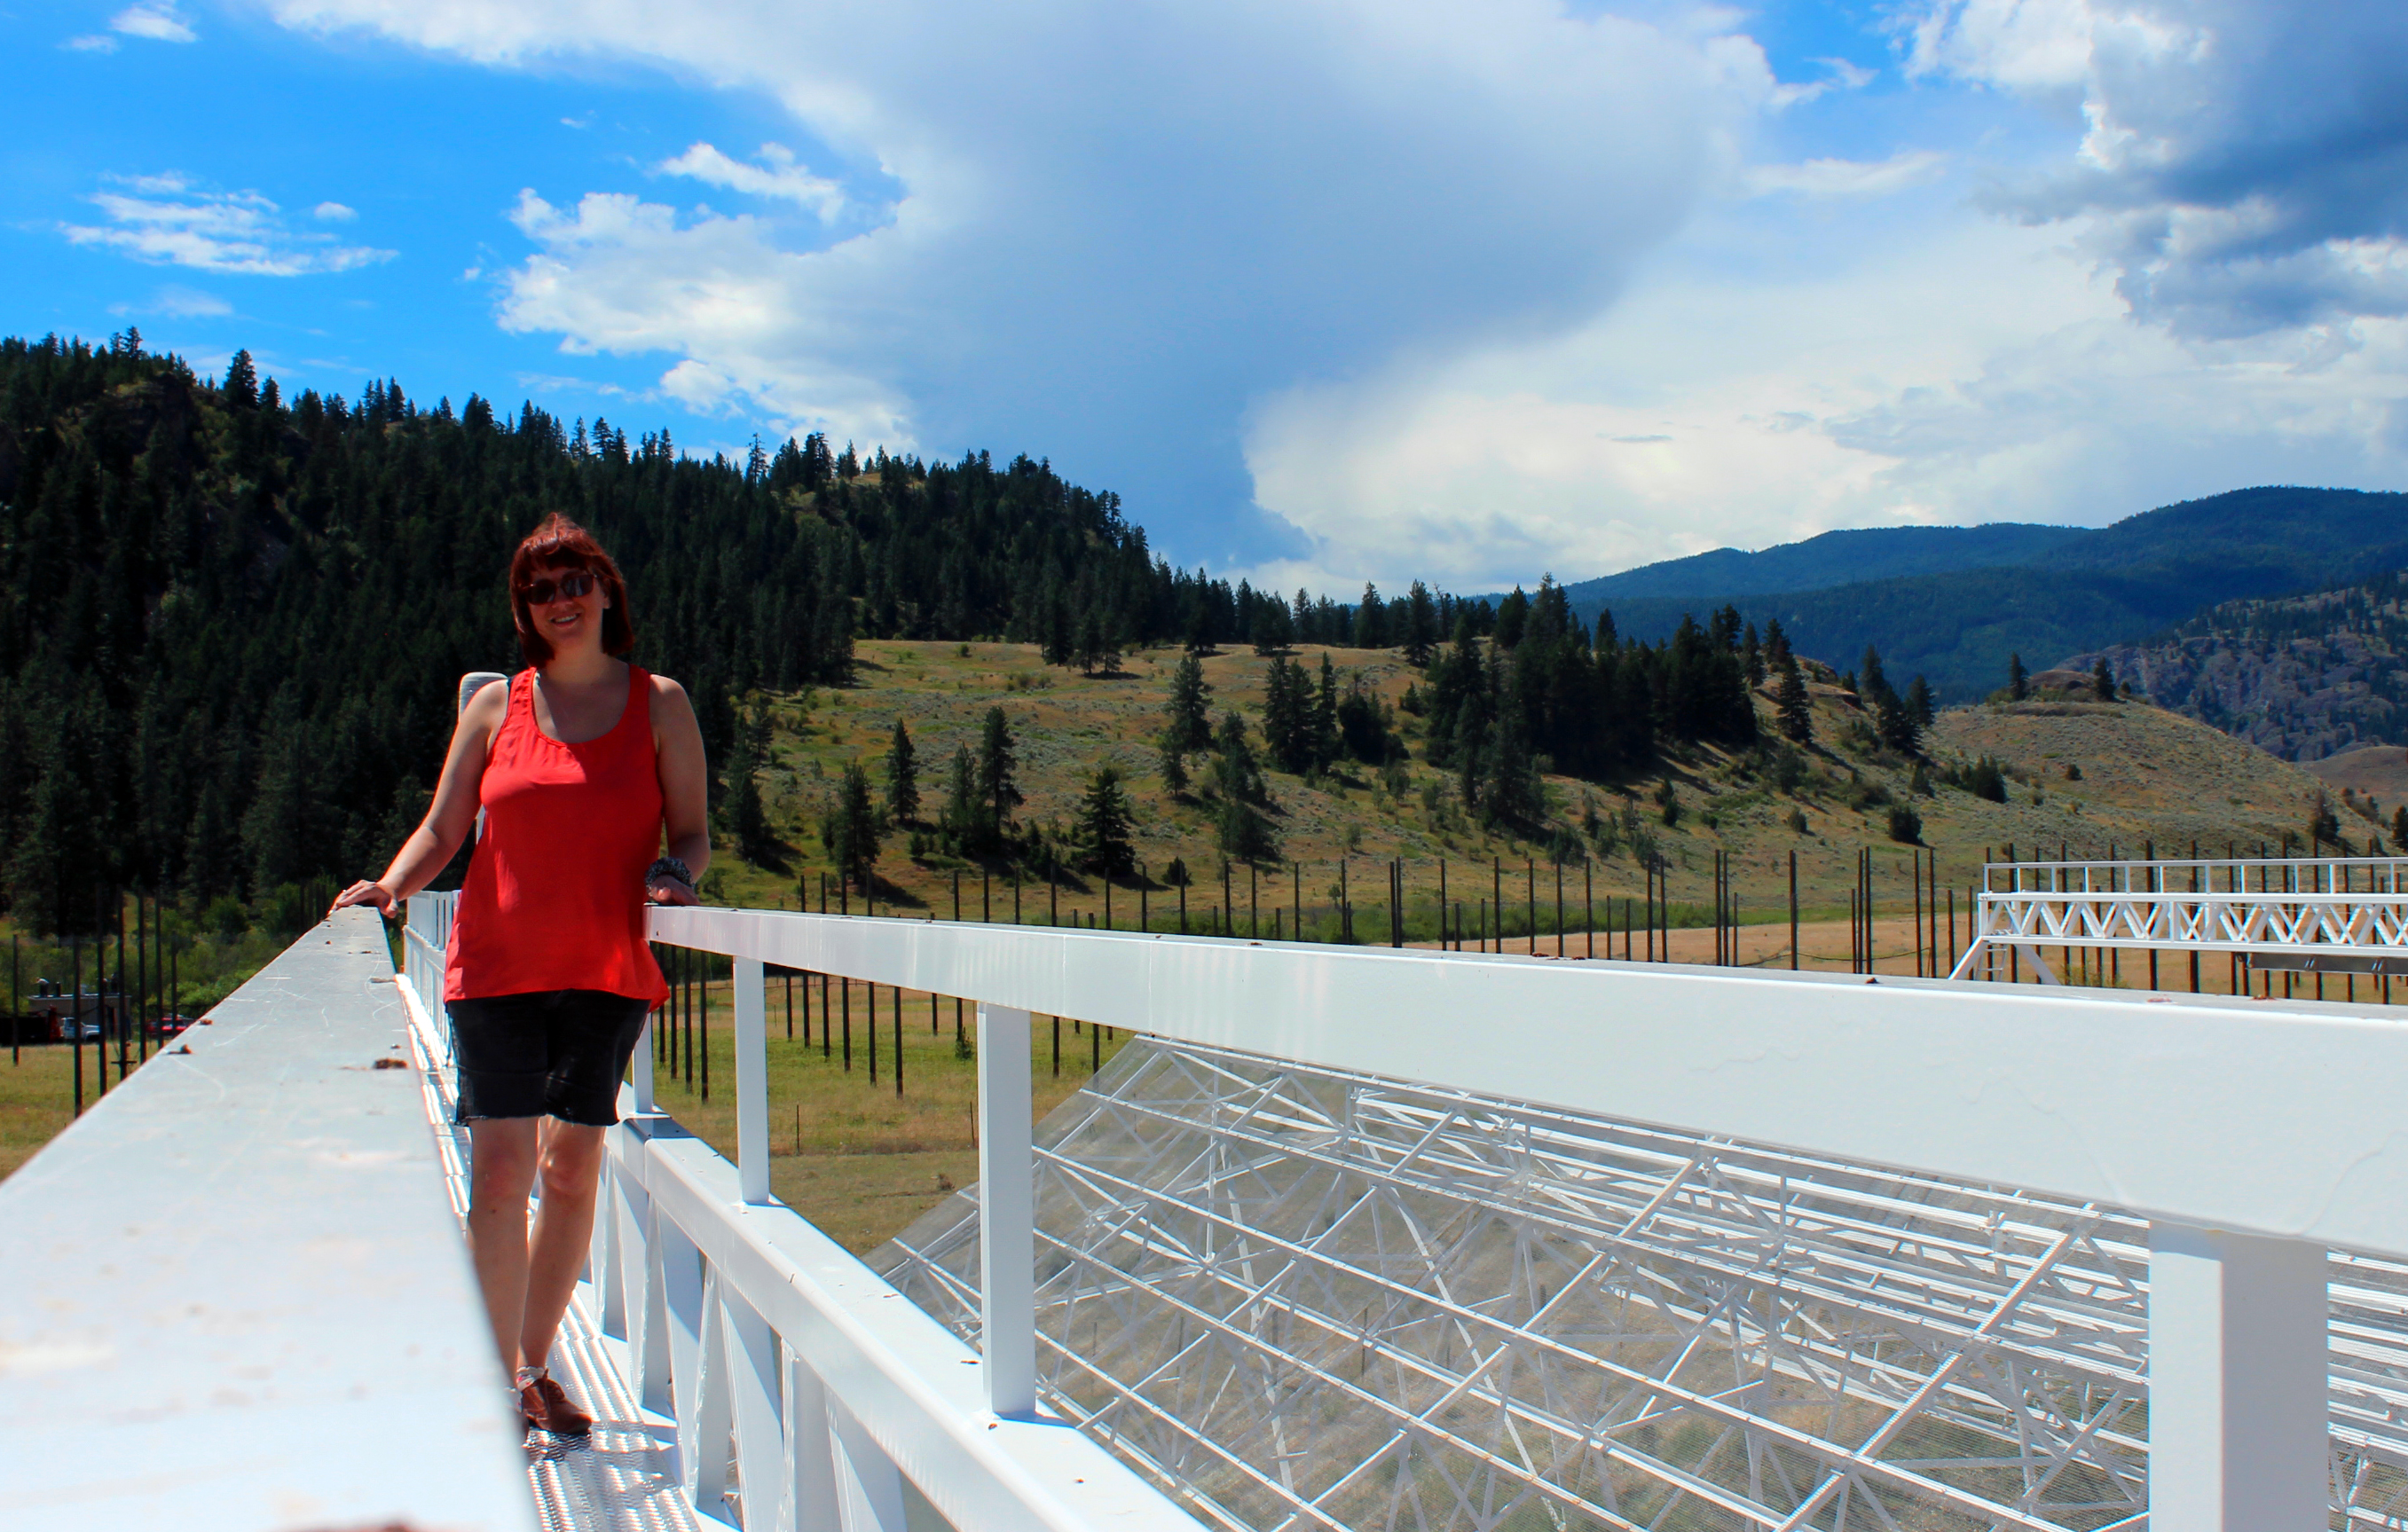
\includegraphics[width=0.95\linewidth]{Planetarium/figures/Filming_at_CHIME.jpg}
\caption{Tabitha on top of one of the CHIME cylinders during filming. }
\label{Fig:CHIME_film}
\end{minipage}%
\begin{minipage}[b]{0.02\textwidth}
\hspace{1cm}
\end{minipage}%
\begin{minipage}[b]{0.37\textwidth}
\centering
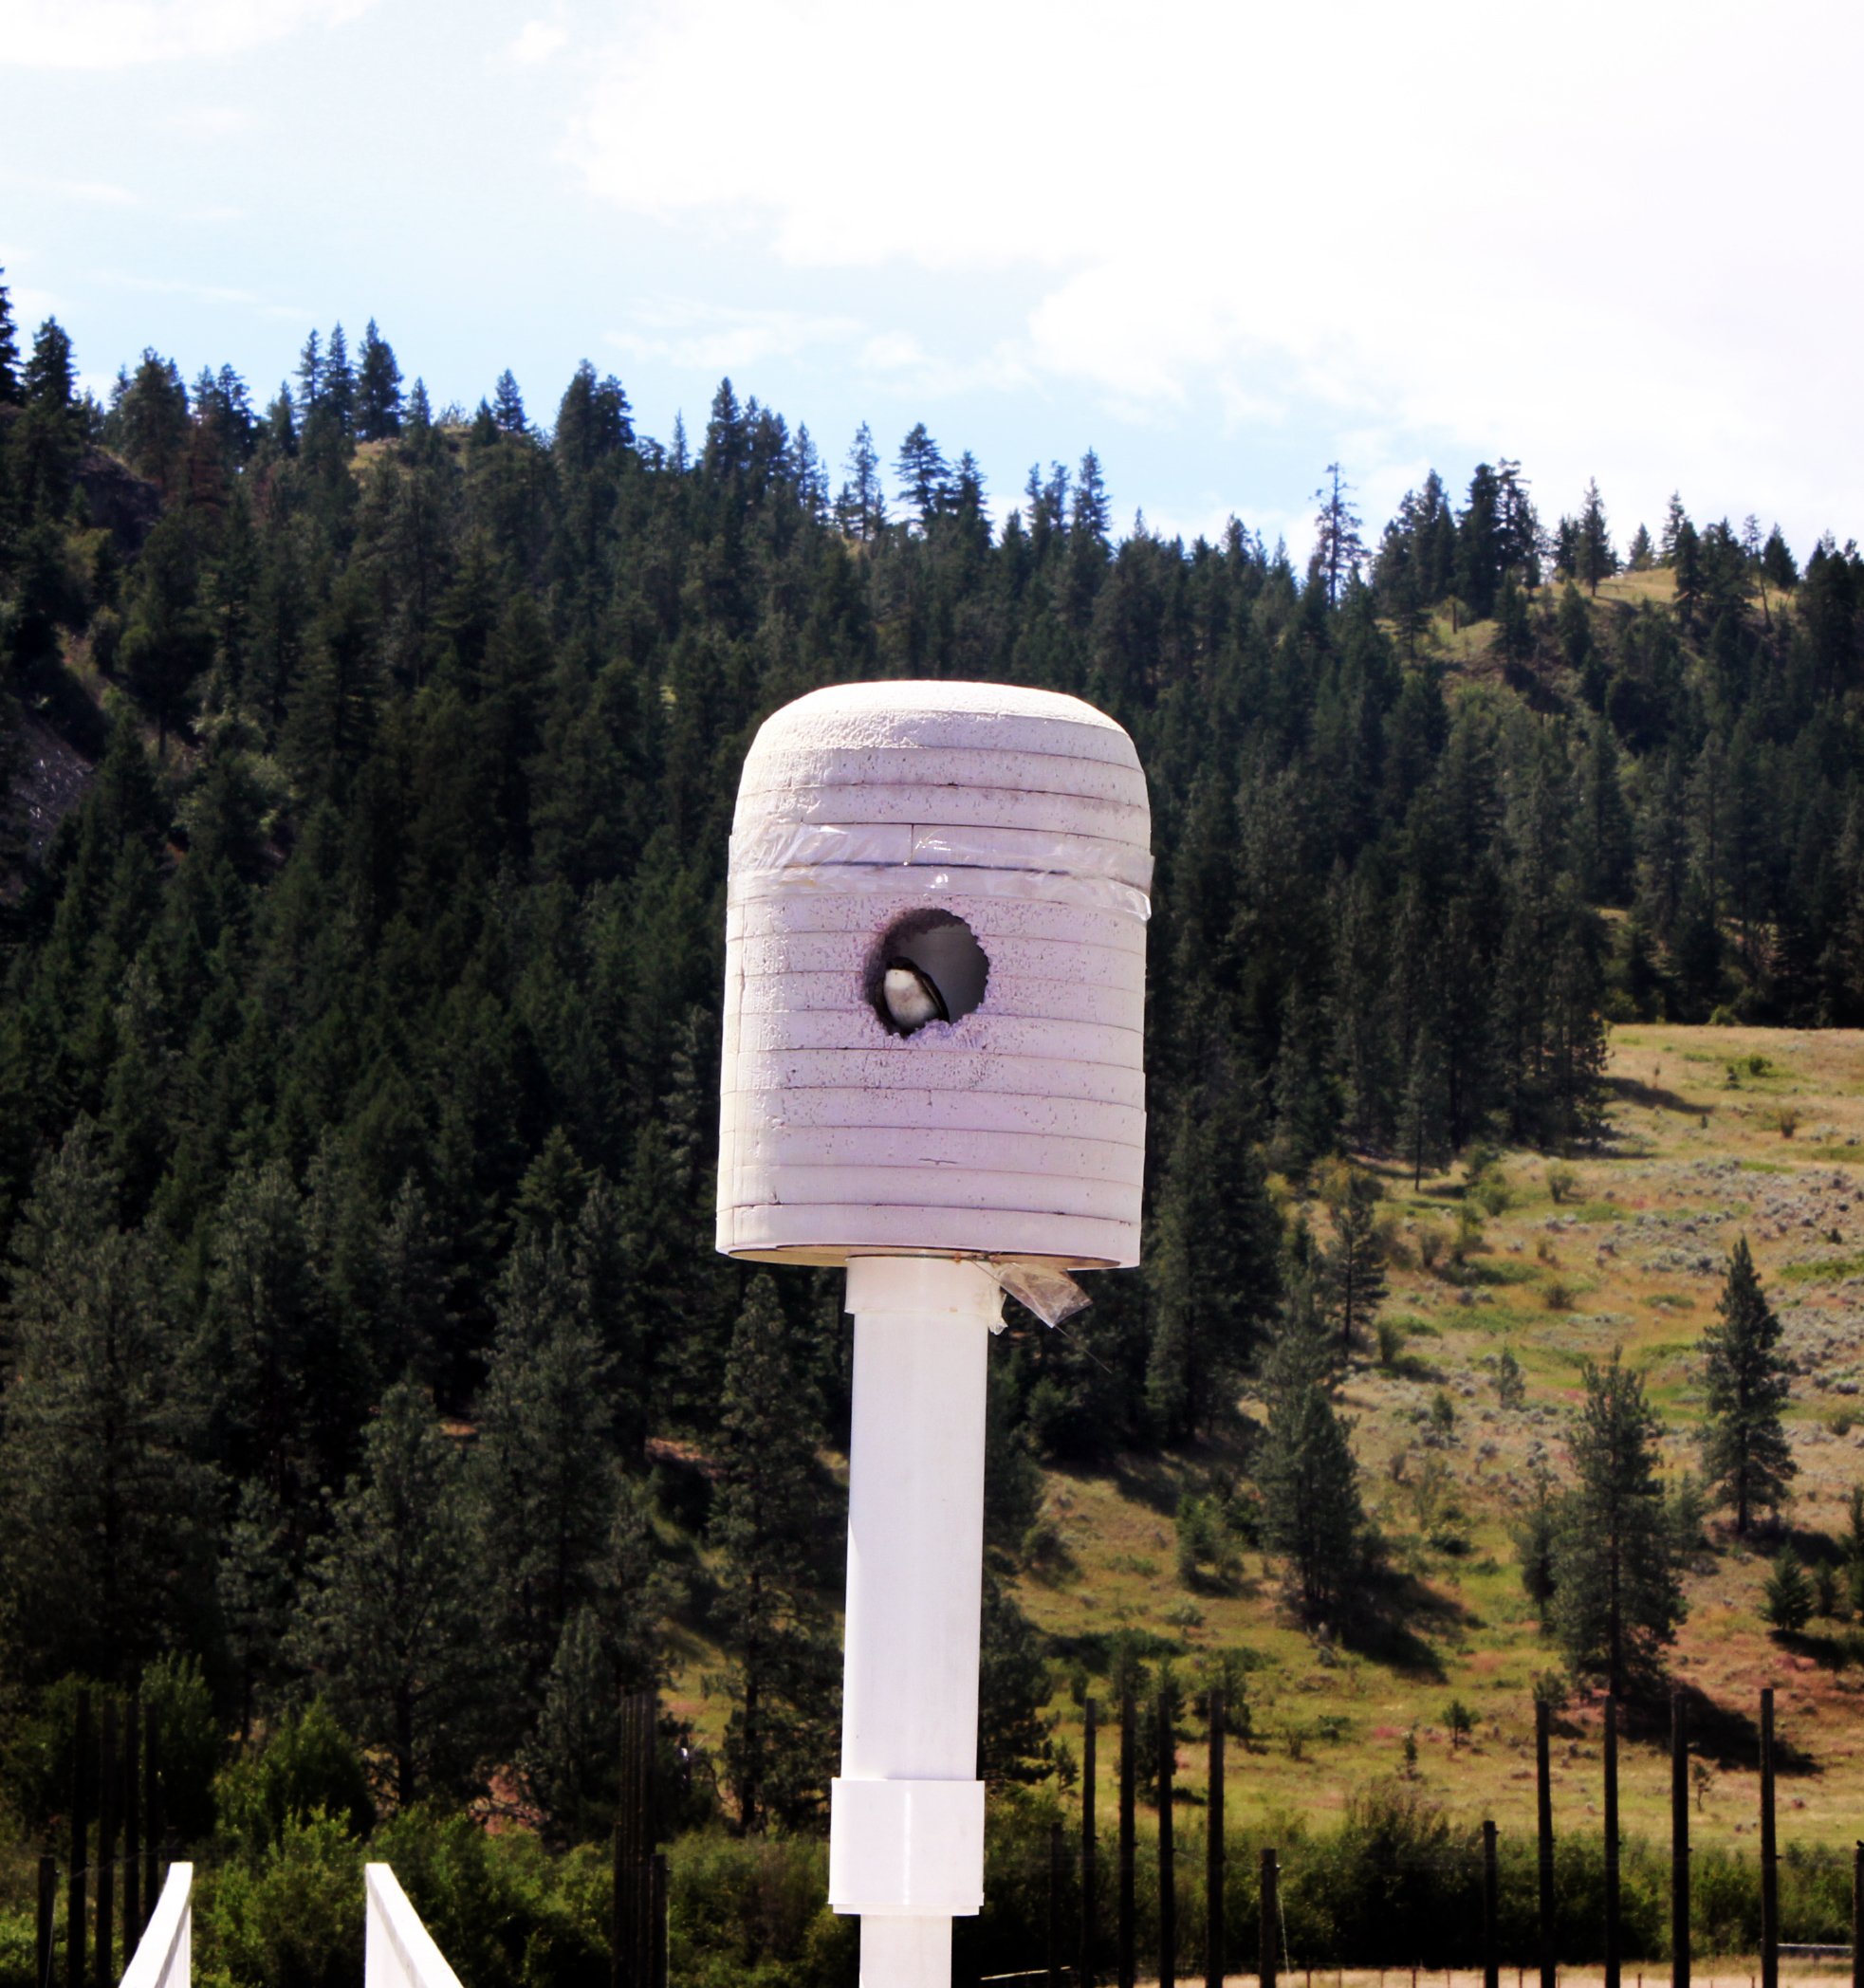
\includegraphics[width=0.95\linewidth]{Planetarium/figures/CHIME_birdsnest.jpg}
\caption{Starlings hollowed out this nest in an RFI antenna on one of the CHIME cylinders.}
\label{Fig:CHIME_bird}
\end{minipage}
\end{figure}

\begin{figure}[htb]
\begin{center}
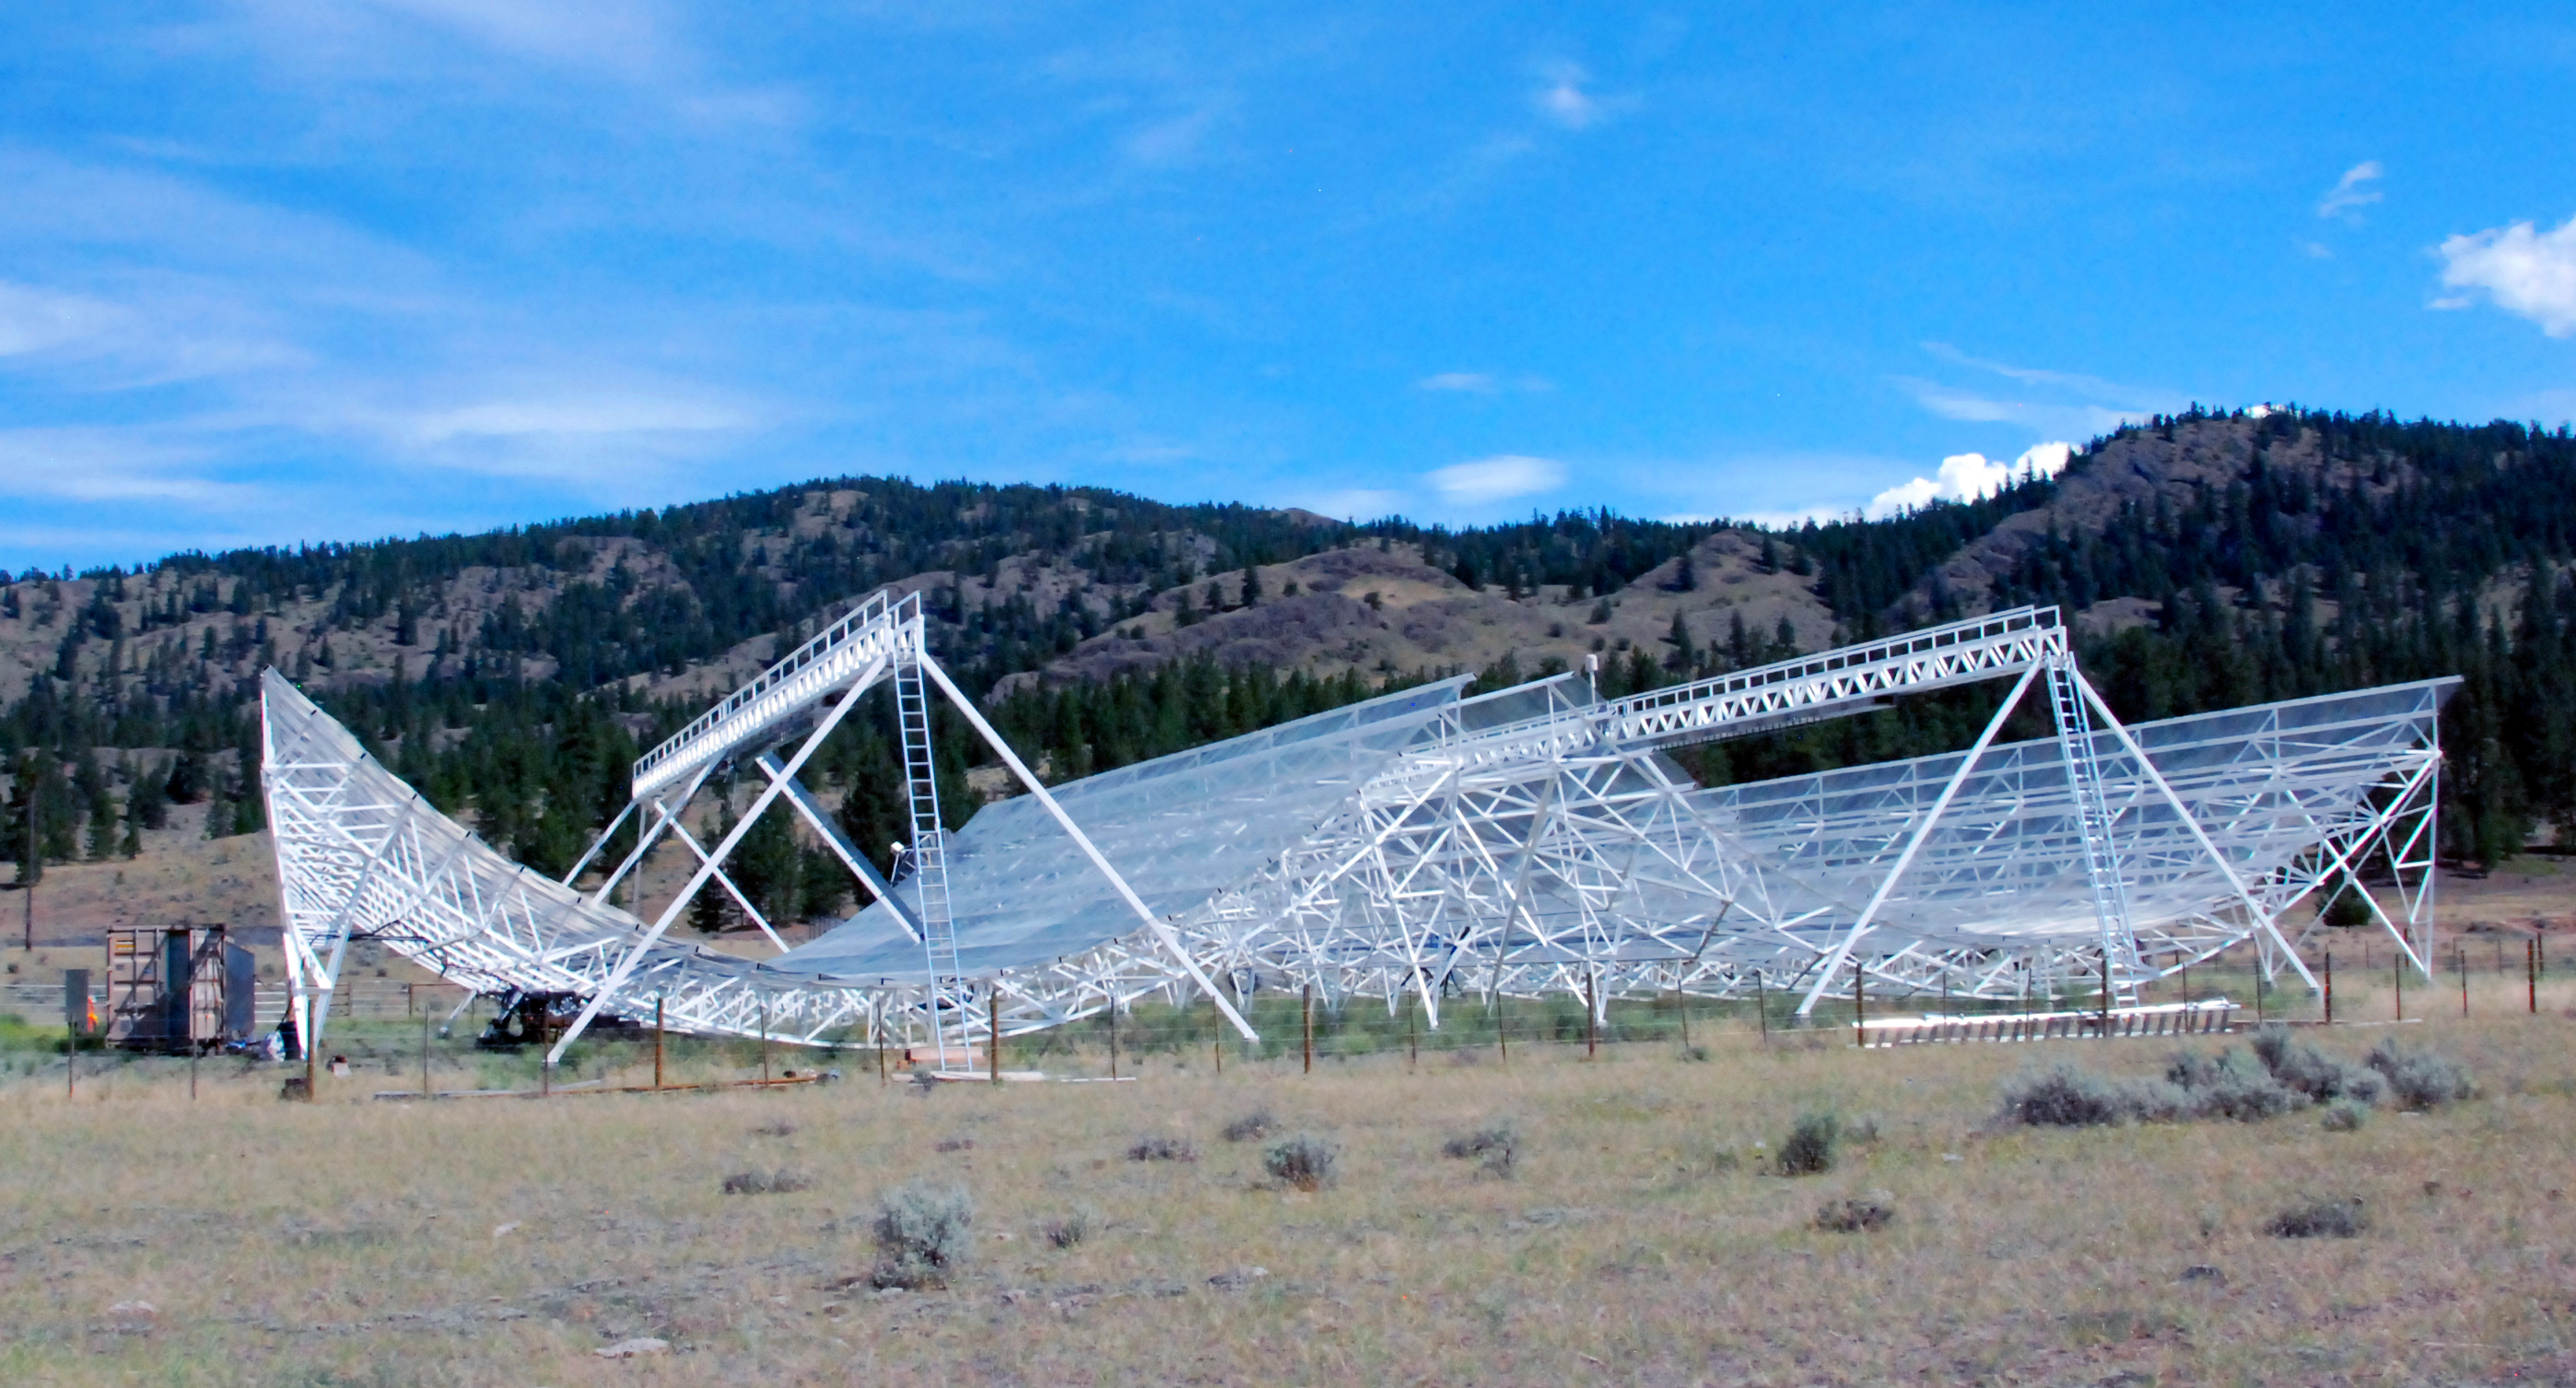
\includegraphics[width=0.95\linewidth]{Planetarium/figures/CHIME_cylinders.jpg}
\caption{CHIME pathfinder cylinders, captured with the rectangular lens. CHIME control room is inside the shipping container on the left side of the cylinders.}
\label{Fig:CHIME_cyl}
\end{center}
\end{figure}

\begin{figure}[htb]
%\begin{center}
\centering
\begin{minipage}[b]{0.54\textwidth}
\centering
\includegraphics[width=0.95\linewidth]{Planetarium/figures/CHIME_cyl_fisheye.png}
\caption{Close up view of one of the CHIME cylinders, captured with the fisheye lens.}
\label{Fig:CHIME_cyl_fisheye}
%\end{center}
%\end{figure}
\end{minipage}%
\begin{minipage}[b]{0.02\textwidth}
\hspace{1cm}
\end{minipage}%
\begin{minipage}[b]{0.42\textwidth}
\centering
%\begin{figure}[htb]
%\begin{center}
\includegraphics[width=0.95\linewidth]{Planetarium/figures/CHIME_dusk_fisheye.jpg}
\caption{CHIME cylinders at dusk, along with the neighboring 26 m dish, captured with the fisheye lens.}
\label{Fig:CHIME_dusk_fisheye}
%\end{center}
\end{minipage}
\end{figure}


\subsection{Penticton, BC, Canada}

In June 2014, Alex and I visited the Dominion Radio Astrophysical Observatory (DRAO) site near Penticton in British Columbia, Canada where the CHIME telescope pathfinder is located and the full CHIME telescope will be built. We stayed locally in the city of Penticton and were able to capture footage despite battling with rain for part of our visit. We were able to capture footage while the CHIME team was working on the computer system so that we didn't interfere with observations. 

Permission to film at the site was provided by Tom Landecker, the primary CHIME contact at the DRAO, as well as the rest of the CHIME team. David Hanna from McGill University was able to show us around the site and get us access during off hours so that we could film around dusk. Figure \ref{Fig:CHIME_film} shows telescope during filming, while Figures \ref{Fig:CHIME_cyl}, \ref{Fig:CHIME_cyl_fisheye}, and \ref{Fig:CHIME_dusk_fisheye} show some of the images we were able to capture at the site with both the rectangular and fisheye lenses. 

\begin{figure}[htb]
\begin{center}
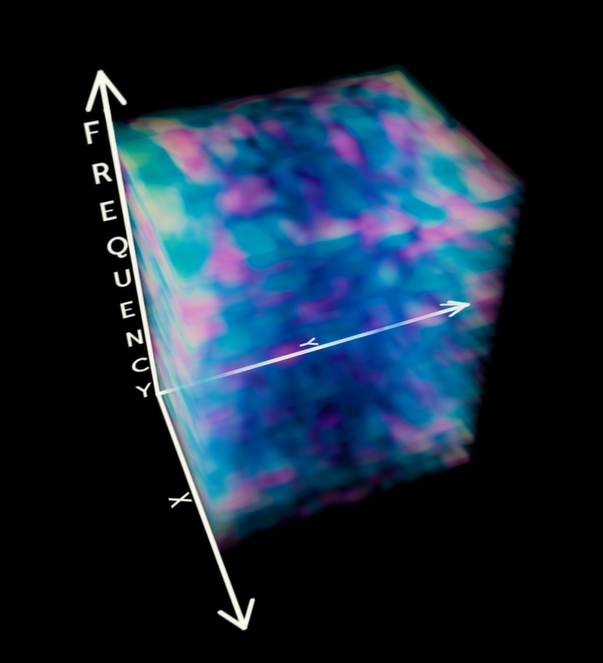
\includegraphics[width=0.95\linewidth]{Planetarium/figures/GBT_cm_map.jpg}
\caption{Map of the Green Bank Telescope Intensity Mapping project $''$deep$''$ field after foreground subtraction. In the image, X and Y are the Right Ascension and Declination of the data (centered at $14^h 31^m 28.5^s$ RA and $2^\circ 0'$ Dec). }
\label{Fig:GBT_cm_map}
\end{center}
\end{figure}



\section{\cm Data Maps}

Because the show is all about the Hydrogen sky, we wanted to be able to show images of that sky. However, there isn't currently a large map of the \cm sky at cosmological redshifts. Instead, we decided to use a combination of data and simulation to show what the Hydrogen sky should look like.

We started with some of the data from the Green Bank Telescope Intensity Mapping project \cite{masui_2012}\cite{switzer_2013}, which looked at a small part of the sky and made maps of the \cm signal with foregrounds. The project used principal component analysis to remove most of the foregrounds, leaving residuals that contain the \cm signal. Figure \ref{Fig:GBT_cm_map} shows a 3D representation of one of these foreground subtracted maps (the 15hr $''$deep$''$ field), which contains the Hydrogen sky for an area of a few square degrees. 

\begin{figure}[htb]
\begin{center}
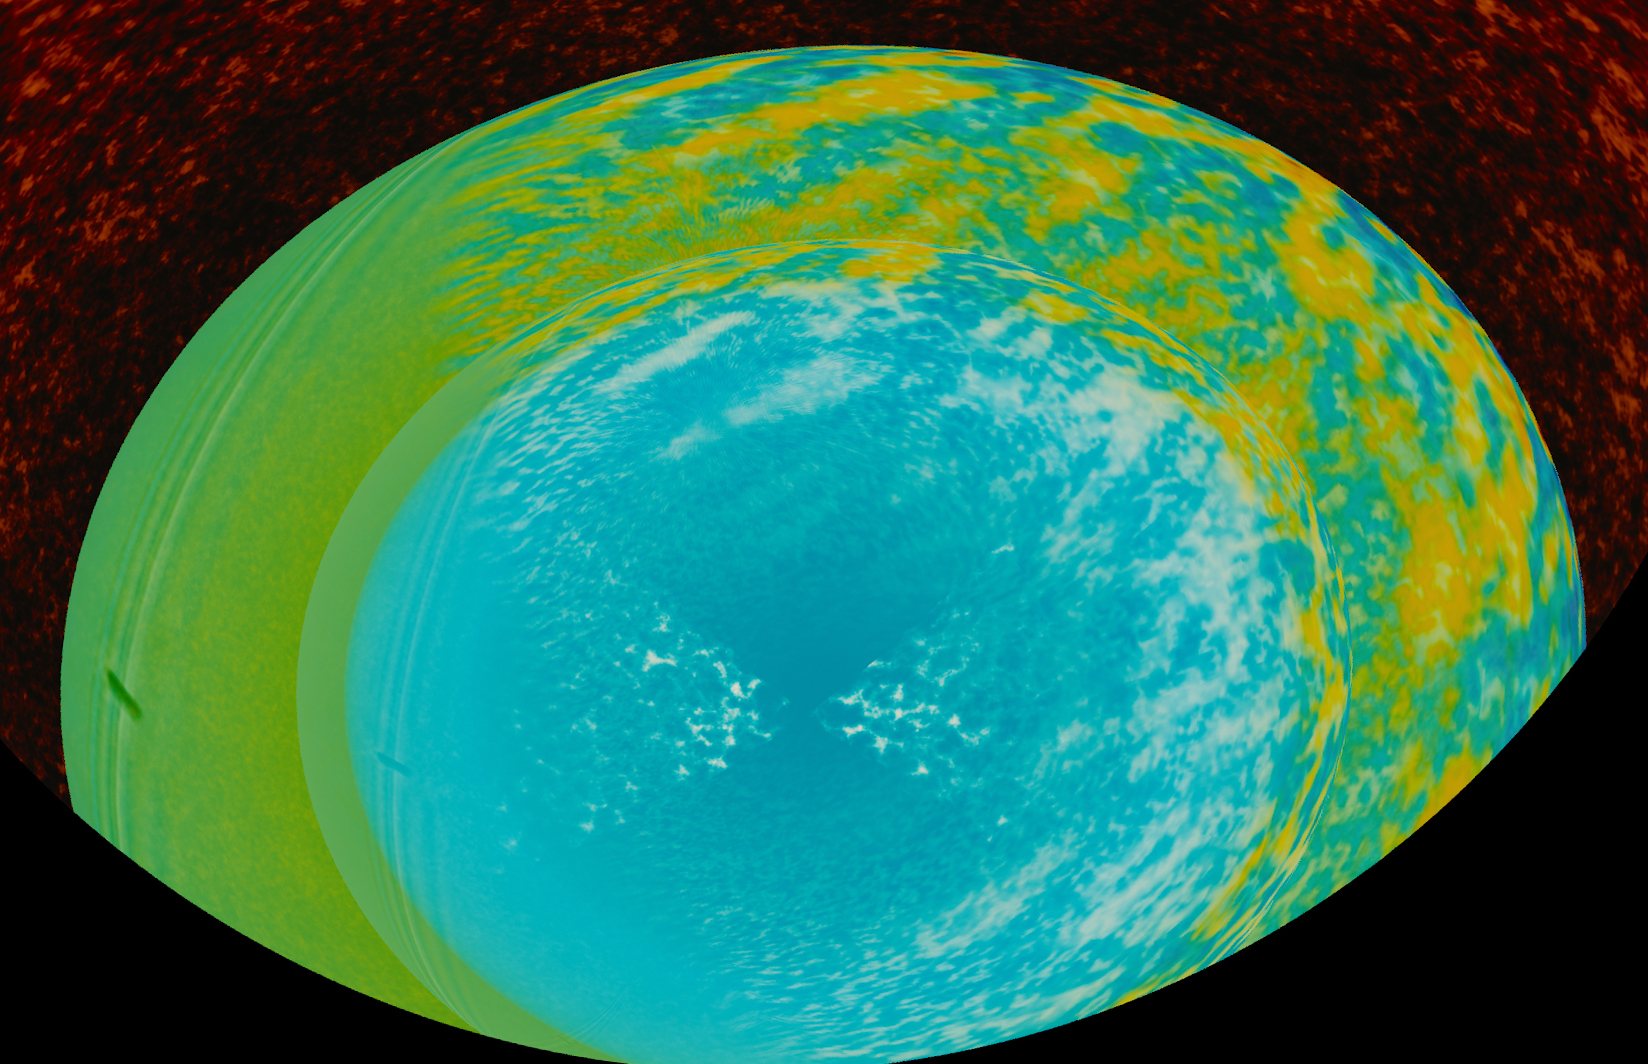
\includegraphics[width=0.95\linewidth]{Planetarium/figures/CHIME_cm_map.jpg}
\caption{Simulated CHIME map in green with blue and yellow temperature variation placed in a shell for the planetarium show. Image center has a model of the large scale structure we've seen so far with optical telescopes, and the red structure along the edge represents the Cosmic Microwave Background.  }
\label{Fig:CHIME_cm_map}
\end{center}
\end{figure}

For the CHIME segment of the show, we decided to use simulated data to show what we expect the Hydrogen sky data to look like. We were given simulated CHIME \cm maps made by Richard Shaw \cite{shaw_2014} to use to create images. These simulations are of the \cm residuals after foreground removal, in the same way that the GBT maps are data residuals after foreground removal. Figure \ref{Fig:CHIME_cm_map} show the simulated CHIME maps as they are used in the planetarium show, placed in a shell corresponding to the redshifts that the maps cover. 



\section{Working in the Planetarium Environment}

One of the big challenges of this project was learning how to work in a planetarium environment, and how it differs from normal video production. Typical planetariums have a $''$2k$''$ or $''$4k$''$ resolution, with an area of roughly 4-8 million square pixels. This means that any images have to be captured at very high resolution, and any animation takes a long time to render (can take days for a few seconds of data). 


\subsection{Image Distortion}

Beyond sheer size, the planetarium environment also distorts images projected on it because of the shape of the dome. The dome shape means that viewers focus is primarily on the bottom third of the image, while the top third of the image is barely seen since it is behind the viewers. Anything placed along the edge of the image is expanded, while anything in the center of the image is shrunk compared to how it looks on a flat screen. You can see this in Figures \ref{Fig:GBT_dusk_fisheye} and \ref{Fig:CHIME_dusk_fisheye}, where the telescopes sit in the bottom of the image. 

\begin{figure}[htb]
\begin{center}
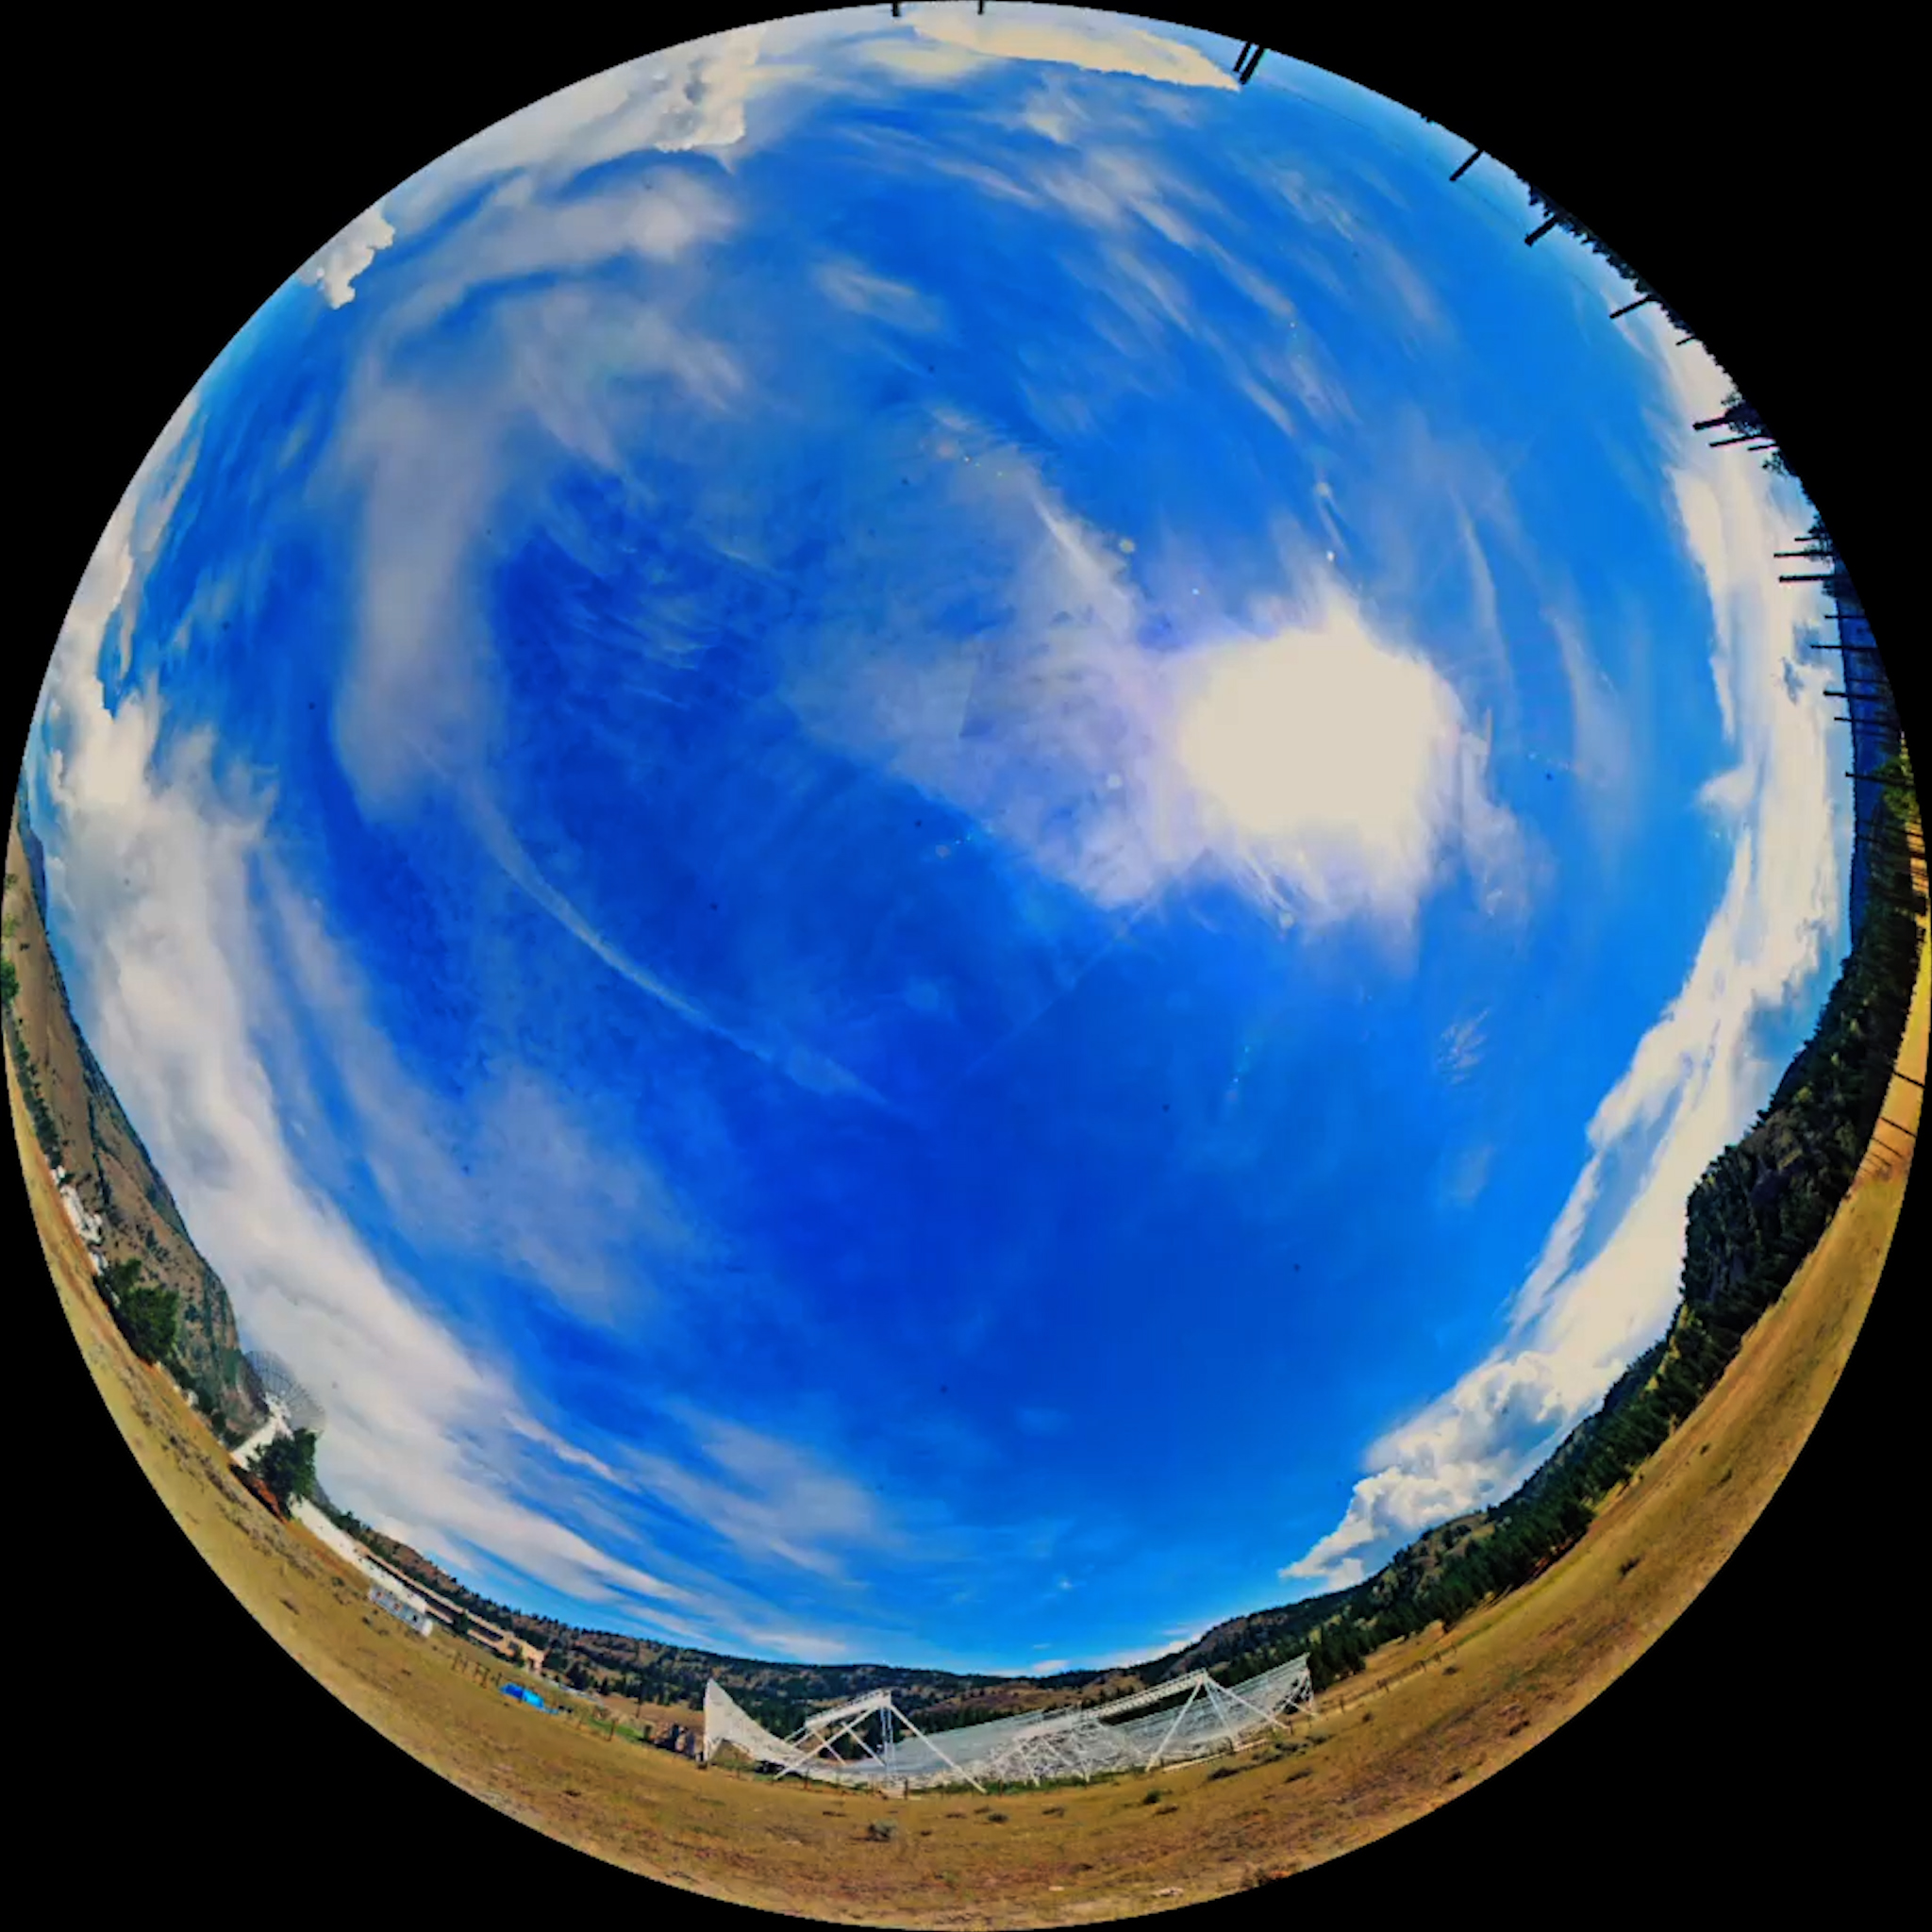
\includegraphics[width=0.95\linewidth]{Planetarium/figures/CHIME_day_dome.jpg}
\caption{Panorama image of the CHIME telescope made using footage shot with the rectangular lens. Color saturation in the image is cranked up to fit the planetarium environment.}
\label{Fig:CHIME_day}
\end{center}
\end{figure}

Image hue and brightness is also different from a regular monitor when viewed on the planetarium screen. If the image is too white or bright, the brightness bleeds into the parts of the image that is supposed to be dark and the image looks washed out. Colors generally tend to look washed out on the dome, so images prepared for the dome should have their saturation cranked up high. In other words, the images should look like they were created with crayons. This can be seen in Figure \ref{Fig:CHIME_day}, where the blue of the sky is much more intense than in the original images. 


\subsection{Motion}

Motion reads differently in a dome environment than it does on a regular screen. Because the dome surrounds so much of a person's vision, if anything is moving too fast it tends to make the viewers nauseous. This means that motion should be at least half as fast as you would use in a regular video. When the whole image moves it needs to be smooth (no hand held camera footage), and motion is best when kept in one direction. We learned this the hard way when we tried to film at the Green Bank Telescope with the fisheye camera. We didn't have a steady cam, but were carrying the camera around while filming. In the dome, the motion caused by the act of walking made the footage unusable; even causing slight nausea during viewing.

Motion can be used quite effectively if you are moving only small parts of the image. Because the rest of the image is still, small objects can move quite fast without causing disorientation. In this case, it is useful to take advantage of the shape of the dome; allowing objects to move in and out of the observer's field of view without leaving the image. In the show, we play with this by having moving Hydrogen atoms with orbiting electrons and photons that travel through the sky. 

\begin{figure}[htb]
\begin{center}
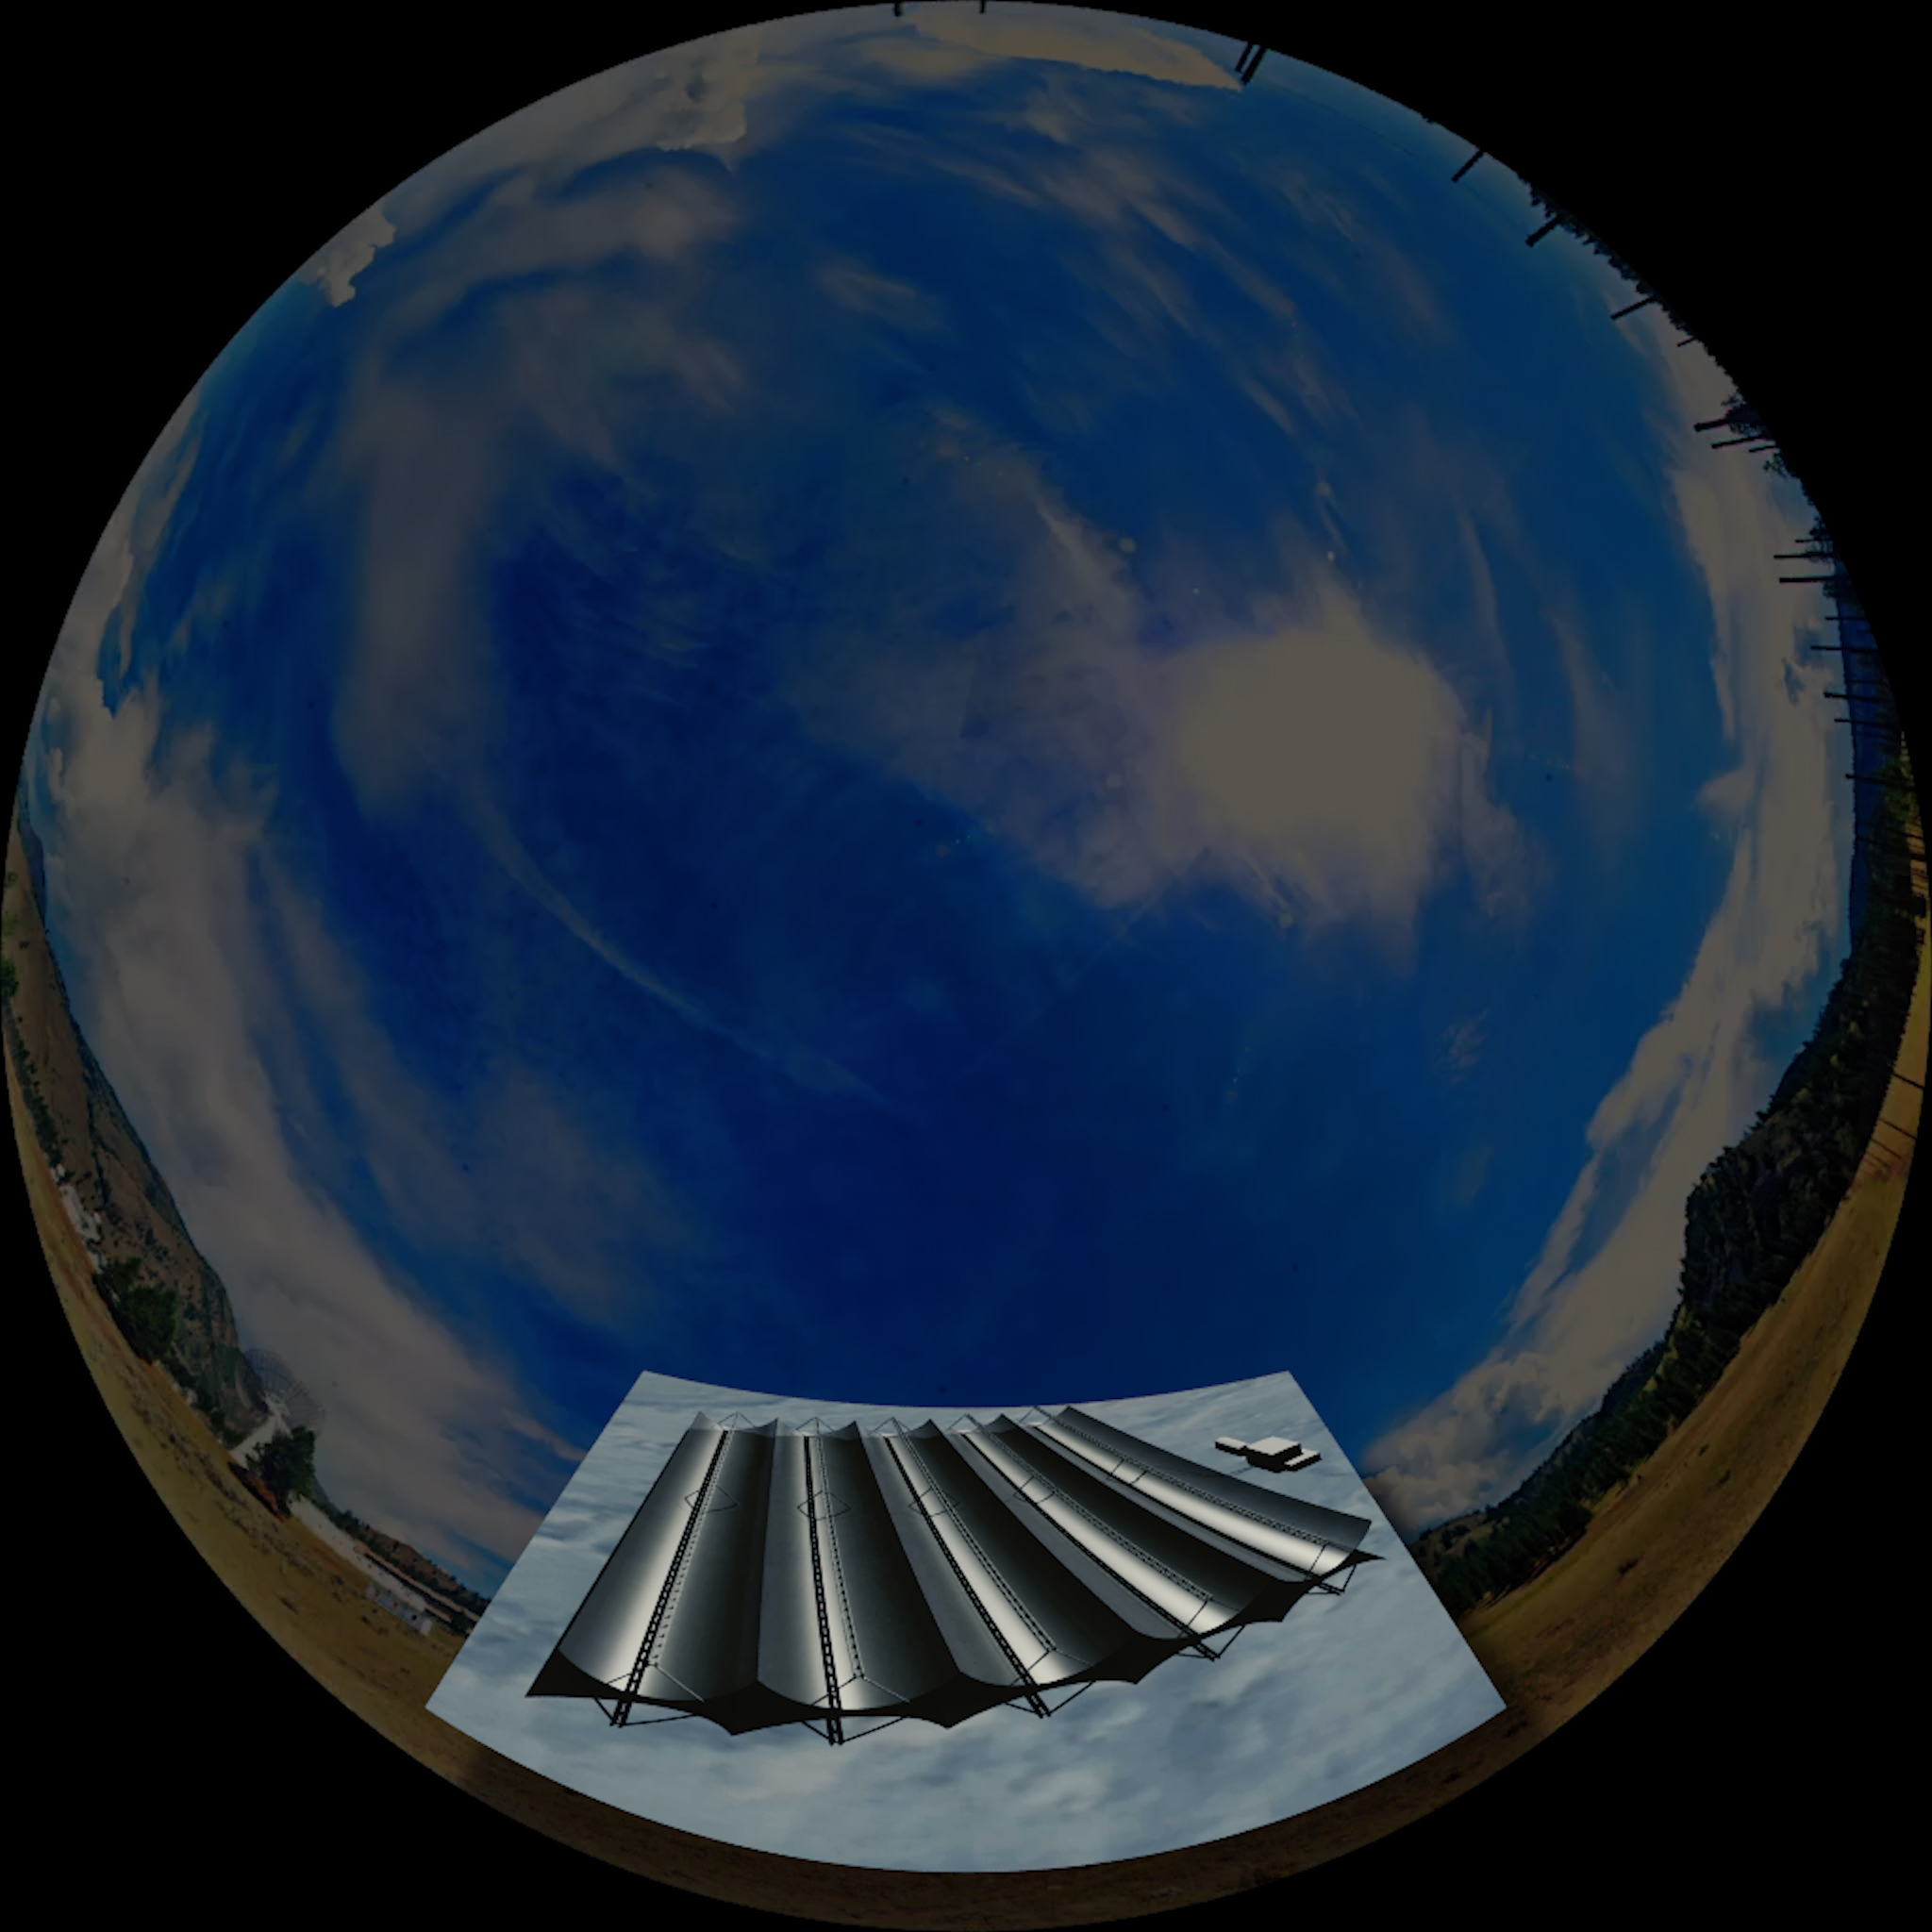
\includegraphics[width=0.95\linewidth]{Planetarium/figures/CHIME_animation.jpg}
\caption{Snapshot of CHIME cylinder animation inside a pop-out with an image of the CHIME telescope as the background.}
\label{Fig:CHIME_animate}
\end{center}
\end{figure}
\subsection{Using pop-outs}

Because creating three-dimensional animation can be quite time consuming and tricky, one common trick that planetarium shows use is pop-out windows. This involves projecting a background image on the dome, then opening a polygon in the bottom center of the image. A two-dimensional animation sequence is run inside the polygon while the background is held constant. 

Figure \ref{Fig:CHIME_animate} shows an example of how we used this for the show, where the animation here is a demonstration of how light interacts with the CHIME cylinders. The snapshot shows a moment when the animation is zoomed out to the full system. We used this technique for our animations that show how light is collected by the different telescopes, CHIME and the Green Bank Telescope. 



\section{Audio Production}

Just as with any other video, sound is an important part of a planetarium show. 
The first part of the sound is the narration. Narrators must speak slowly and clearly and enunciate so that none of the words become garbled. Breath control is also important, in order to avoid audible breaths in the recording. It is also important to speak naturally, and convey enthusiasm for the material. As is indicated by the script, I acted as the show narrator to provide a personal element to the story. 

Usage of sound booth can provide a way to control the environment and avoid environmental noise. It is also important to have a good quality microphone and control the sound levels to avoid clipping. For this show, we were able to use the sound booth at the CMU Entertainment Technology Center to record the narration.  

Beyond the narration, the audio needs depth and complexity. The first step is to add a musical soundtrack behind the narration. This music should be set low enough not to drown out the narrator, but can become dominant during pauses in the narration. Narrative pauses are important, as they give the audience a chance to process what they've just heard. These pauses can also give the audience a chance to focus on the visuals. 

Sound effects can be added to the soundtrack to match the action on the screen and further emphasize the visual story. Such auditory queues help the audience understand what they are seeing. For all of these components, it is particularly important that the sound and audio match. If the narration doesn't match what is happening on the screen, the audience can become lost or confused. With the level of technical detail present in our show, we had to be particularly careful with our synchronization as even a few seconds makes a big difference in comprehension. 


\section{Feedback and Evaluation}

One of the most important parts of any show is getting feedback from various audiences. This is particularly important in a planetarium show, where the goal is to reach and educate the public. Feedback can take many forms and should occur throughout the development process. 


\subsection{Process Feedback}

\subsubsection{Concept Review}

The first stage of feedback was getting approval for our concept. After we had created a rough storyboard, we took the story to Jeff Peterson and Peter Timbie, the principal investigators for the NSF grant funding the project. We identified our primary goals for the project: to educate the public about the Hydrogen sky as a new way to see the universe and how we are able to use radio telescopes to see the Hydrogen sky. 

\subsubsection{Planetarium Testing}

Throughout the project, we needed to test our footage in the planetarium environment. This was important because it allowed us to see what things looked like in the planetarium compared to the flat screen and make adjustments. In addition, this gave us the opportunity to meet regularly with Tom Casey and Frank Mancuso, who acted as technical advisors for the project. 


\subsection{Script Development}

In writing the script, one of the big challenges was describing technical and scientific details in language that would be accessible to the general public. The rule of thumb for planetarium shows is to write toward a middle school audience comprehension level. When writing the script, it was important to capture the ideas with analogies that would be accessible, and to match the visual story being told. 

We went through several iterations of the script, including multiple recordings of the narration. One of the things that we found was that sometimes a line that made sense on paper didn't translate right when spoken. We also got feedback on the script from both scientists and educators, including Dr. Brendan Mullen at the Carnegie Science Center. 

Because of the length and goals of the show, we ended up with a more technical show that is suitable for high-school and college age students. While this wasn't our original intent, the focus on the why and how behind \cm cosmology ended up being better suited for an older audience. 


\subsection{Intermediate Viewings}

Once we had a show that was mostly complete, we went through a number of intermediate viewings. In these viewings, we invited some of our advisors to come and see the show and give recommendations of what we should change or keep. We tried to get advice from different perspectives, including technical details, creative and storytelling feedback, and scientific accuracy. These viewings helped us to revise the show and create a coherent story that worked together. 


\subsection{Public Viewings}

A preview of the completed show can be viewed online (http://youtu.be/4E5luX1dCtA). At this time it is not yet available for public viewing, but we plan to have an open showing at the Carnegie Science Center in 2015. Following the viewing, we plan to ask viewers to give feedback via a survey. The exact form of this survey is still under development. 

Getting public feedback will help us to assess the success of our show in meeting the stated goal of educating the public on the Hydrogen Sky. The show may also be used as a pilot for a full size show ($\sim 30-60$ minutes) as \cm science efforts continue to expand and larger \cm map datasets become available. 
